%%%%%%%%%%%%%%%%%%%%%%%%%%%%%%%%%%%%%%%%%
% The Legrand Orange Book
% LaTeX Template
% Version 3.1 (February 18, 2022)
%
% This template originates from:
% https://www.LaTeXTemplates.com
%
% Authors:
% Vel (vel@latextemplates.com)
% Mathias Legrand (legrand.mathias@gmail.com)
%
% License:
% CC BY-NC-SA 4.0 (https://creativecommons.org/licenses/by-nc-sa/4.0/)
%
% Compiling this template:
% This template uses biber for its bibliography and makeindex for its index.
% When you first open the template, compile it from the command line with the 
% commands below to make sure your LaTeX distribution is configured correctly:
%
% 1) pdflatex main
% 2) makeindex main.idx -s indexstyle.ist
% 3) biber main
% 4) pdflatex main x 2
%
% After this, when you wish to update the bibliography/index use the appropriate
% command above and make sure to compile with pdflatex several times 
% afterwards to propagate your changes to the document.
%
%%%%%%%%%%%%%%%%%%%%%%%%%%%%%%%%%%%%%%%%%

%----------------------------------------------------------------------------------------
%	PACKAGES AND OTHER DOCUMENT CONFIGURATIONS
%----------------------------------------------------------------------------------------

\documentclass[
	12pt, % Default font size, select one of 10pt, 11pt or 12pt
	%fleqn, % Left align equations
	a4paper, % Paper size, use either 'a4paper' for A4 size or 'letterpaper' for US letter size
	oneside, % Uncomment for oneside mode, this doesn't start new chapters and parts on odd pages (adding an empty page if required), this mode is more suitable if the book is to be read on a screen instead of printed
]{LegrandOrangeBook}

% Book information for PDF metadata, remove/comment this block if not required 
\hypersetup{
	pdftitle={Introdução à Matemática Superior}, % Title field
	pdfauthor={Jordan Lambert}, % Author field
	pdfsubject={Apostila}, % Subject field
	pdfkeywords={IMS, Pré-Cálculo, ...}, % Keywords
	pdfcreator={LaTeX}, % Content creator field
}

\addbibresource{sample.bib} % Bibliography file

\definecolor{ocre}{RGB}{16,85,154} % Define the color used for highlighting throughout the book

\let\cleardoublepage\clearpage

%%%%%%%%%%%%%%%%%%%%%%%%%%%%%%%%%
%   Opcões de Linguagem
%%%%%%%%%%%%%%%%%%%%%%%%%%%%%%%%%
\usepackage[english,brazil]{babel} %fazemos com que o compilador traduza expressões como “table of contents”
\usepackage{csquotes}
\usepackage[utf8]{inputenc}
\usepackage[T1]{fontenc}


%\usepackage{fancyhdr}
%\pagestyle{fancy}
%\fancyhf{}
%\fancyhead[RE]{Introdução à Matemática Superior}
%\fancyhead[LO]{\rightmark}
%\fancyhead[LE,RO]{\thepage}

%license footnote
\cfoot{\tiny{Licença \href{https://creativecommons.org/licenses/by-sa/4.0/}{CC BY-SA-4.0}.}}

%\usepackage[fixlanguage]{babelbib}
%\selectbiblanguage{brazil}

%%%% ams-latex %%%%
\usepackage{amsmath}
\usepackage{amssymb}
\usepackage{amsthm}
\usepackage{amsfonts}
\usepackage{comment}
%%%% graphics %%%%
\usepackage{graphicx} % Possibilita o uso de figuras e gráficos (suporta os formatos EPS, PDF, JPG e PNG)
%\usepackage{caption}

%%%% links %%%%
%\usepackage[colorlinks=true, allcolors=blue]{hyperref}   %usado para incluir links no texto

%%%% indent first line %%%%
\usepackage{indentfirst}

%%%% citation %%%%
%\usepackage{cite}               % usado para citações

%%%% lists %%%%
\usepackage{enumerate}          % para fazer listas com tipos diferentes de itens (a, i, 1,...)

%%%% index %%%%
%\usepackage{makeidx}            % índice remissivo

%%%% links %%%%
%\usepackage[colorlinks=true, allcolors=blue]{hyperref}   %usado para incluir links no texto

%%%% miscellaneous %%%%
\usepackage{multicol}
\usepackage{multirow}           % para tabelas, basicamente essencial
\usepackage[normalem]{ulem}     %para riscar palavra usando \sout
\usepackage{calrsfs}
\usepackage{subfigure}           %para colocar figuras lado a lado
\usepackage{xcolor}
\usepackage{tikz,tkz-base,tkz-fct}              % para criar desenhos legais
\usetikzlibrary{fit,shapes.geometric,arrows,shadows.blur, angles} %pra fazer os diagramas de funções
\usepackage{colortbl}
\usepackage{cleveref}

\usepackage{textcomp}
\usepackage{gensymb} %usar comando \degree
\usepackage{venndiagram}

\usepackage{shadethm}
\usepackage{bm}

\usepackage{float}
\usepackage{tasks}

\usepackage{longtable}

\setlength{\marginparwidth}{2cm}
\usepackage{todonotes}

\usepackage{polynom} %divisão de polinômios


\newcommand{\fim}{\hfill {$\Box$}}
\newcommand{\destaque}[1]{\colorbox{ocre!50}{$\displaystyle #1$}}
\newcommand{\iu}{{i\mkern1mu}} %unidade imaginária
\newcommand{\sen}{\operatorname{sen}}
\newcommand{\cotan}{\operatorname{cot}}
\newcommand{\cosec}{\operatorname{csc}}
\newcommand{\arcsen}{\operatorname{arcsen}}
\newcommand*\abs[1]{\left|#1\right|}

\DeclareMathOperator{\tg}{tg}
\DeclareMathOperator{\cotg}{cotg}
\DeclareMathOperator{\cossec}{cossec}
\DeclareMathOperator{\arctg}{arctg}

%\newcommand{\exemautorefname}{Exemplo}
%\newcommand*{\propautorefname}{Proposição}

\newcommand{\N}{\mathbb{N}}
\newcommand{\Z}{\mathbb{Z}}
\newcommand{\Q}{\mathbb{Q}}
\newcommand{\I}{\mathbb{I}}
\newcommand{\R}{\mathbb{R}}
\newcommand{\C}{\mathbb{C}}

\renewcommand{\geq}{\geqslant}
\renewcommand{\leq}{\leqslant}

\newcommand{\paralela}{\hspace{3pt}/\hspace{-2pt}/\hspace{3pt}}
\newcommand{\eqline}{\noalign{\smallskip} \hline \noalign{\smallskip}}

\chapterimage{fundo_triang.png} % Chapter heading image
\chapterspaceabove{6.5cm} % Default whitespace from the top of the page to the chapter title on chapter pages
\chapterspacebelow{6.75cm} % Default amount of vertical whitespace from the top margin to the start of the text on chapter pages

\newenvironment{sol}
{\let\oldqedsymbol=\qedsymbol
  \renewcommand{\qedsymbol}{$\Diamond$}
  \begin{proof}[\bfseries\upshape Solução]}
  {\end{proof}
  \renewcommand{\qedsymbol}{\oldqedsymbol}}

%%%%%%%%%%%%%%%%%%%%%%%%%%%%%%
% Exercícios Resolvidos
%%%%%%%%%%%%%%%%%%%%%%%%%%%%%%
\newtheorem{exeresol}{ER}[section]
\newenvironment{resol}
{\let\oldqedsymbol=\qedsymbol
  \renewcommand{\qedsymbol}{$\Diamond$}
  \begin{proof}[\bfseries\upshape Solução]}
  {\end{proof}
  \renewcommand{\qedsymbol}{\oldqedsymbol}}
%%%%%%%%%%%%%%%%%%%%%%%%%%%%%%

% \newenvironment{dem}[1][\textbf{Demonstração:} \ ]{\textbf{#1}}{\hfill\rule{2mm}{2mm}}

%----------------------------------------------------------------------------------------


\usetikzlibrary{arrows.meta,math}
\usepackage{ifthen}
\usepackage{xargs}

\usetikzlibrary {fpu}
\pgfkeys{/pgf/number format/.cd,frac ,frac whole=false,}
\pgfkeys{/pgf/number format/.cd,frac,frac whole=false,/pgf/number format/frac shift=1}

\newcommandx{\realline}[6][3=10000,4=0,5=10000,6=0]
{
    \begin{tikzpicture}[
    line/.style = {draw, ultra thick, shorten <=-2pt},
    real/.style = {black, {{}-{Triangle[length=4pt, line width=1pt]}}},]
                     ]
    \draw[real] (#1-0.5,0) -> (#2+0.5,0) ;%{Triangle[length=4pt, line width=1pt]};    % <---
    \foreach \i in {#1,...,#2} % numbers on line
    \draw[black] (\i,0.1) -- ++ (0,-0.2)    % <---
        node[below,text=black] {$\i$}; % tick and their labels
    
    \tikzmath{
        if #3 != 10000 then {
            {\filldraw [color=black, fill=red, thick] (#3,0) circle (2pt);};
            %if int(#3) != #3 then {
            {\draw (#3,0.1) node[above]{#4};};
            %};
        };
        if #5 != 10000 then {
            {\filldraw [color=black, fill=red, thick] (#5,0) circle (2pt);};
            %if int(#3) != #3 then {
            {\draw (#5,0.1) node[above]{#6};};
            %};
        };
    };
  \end{tikzpicture}
}

\newcommand{\exibir}[1]{
    \tikzmath{
        \w=int(#1);
        if \w==#1 then {print{\w};} else {print{\pgfmathprintnumber{#1}};};
    }
}
   
\newcommand{\intersection}[8]{
\def\x{{#1}}
\def\y{{#4}}
\begin{tikzpicture}[
    line/.style = {draw, ultra thick, shorten <=-2.5pt},
    21/.style = {line, shorten >=-2.5pt,
               {Circle[length=5pt, line width=1pt]}-{Circle[length=5pt,line width=1pt, fill=white]}},
    12/.style = {line, shorten >=-2.5pt,
               {Circle[length=5pt, line width=1pt, fill=white]}-{Circle[length=5pt, line width=1pt]}},
    11/.style = {line, shorten >=-2.5pt,
               {Circle[length=5pt, line width=1pt, fill=white]}-{Circle[length=5pt, line width=1pt, fill=white]}},
    22/.style = {line, shorten >=-2.5pt,
               {Circle[length=5pt, line width=1pt]}-{Circle[length=5pt, line width=1pt]}},
    10/.style = {line, shorten >=-2.5pt,
           {Circle[length=5pt, line width=1pt, fill=white]}-{}},
    20/.style = {line, shorten >=-2.5pt,
           {Circle[length=5pt, line width=1pt]}-{}},
    01/.style = {line, shorten >=-2.5pt,
           {}-{Circle[length=5pt, line width=1pt, fill=white]}},
    02/.style = {line, shorten >=-2.5pt,
           {}-{Circle[length=5pt, line width=1pt]}},
    1/.style = {line, shorten >=-2.5pt,
           {}-{Circle[length=5pt, line width=1pt, fill=white]}},
    2/.style = {line, shorten >=-2.5pt,
           {}-{Circle[length=5pt, line width=1pt]}},
    real/.style = {gray, {{}-{Triangle[length=4pt, line width=1pt]}}},
    ]
    
    \tikzmath{
        let \s=5;
        let \sep=0.8;
        let \m=0.8;
        let \xtype=#2;
        let \ytype=#5;
        let \atype=#7;
        real \xr;
        real \yr;
        %\xr1 = #1;
        %\xr2 = #2;
        \xr1 = \x[0];
        \xr2 = \x[1];
        \yr1 = \y[0];
        \yr2 = \y[1];
        % Min max values
        real \k;
        \k1 = min(\xr1,\xr2,\yr1,\yr2);
        \k2 = max(\xr1,\xr2,\yr1,\yr2);
        real \f;
        % Auxiliar variables
        \f = \s/(\k2-\k1);
        real \g;
        \g = \s/(\k2-\k1)*\k1;
        % Correction
        if (\xtype==01 || \xtype==02) && \xr1>\k1  then {\xr1=\k1;};
        if (\xtype==10 || \xtype==20) && \xr2<\k2  then {\xr2=\k2;};
        if (\ytype==01 || \ytype==02) && \yr1>\k1  then {\yr1=\k1;};
        if (\ytype==10 || \ytype==20) && \yr2<\k2  then {\yr2=\k2;};
        %Function to draw the real lines
        function drawline (\z1,\z2,\type,\cor) {
            if \cor==1 then {let \c=blue;} else {let \c=black;};
            %{\draw node{$\l$}};
            {\draw[real] (-\m,0) -- (\s+\m+0.15,0);};
            if \type!=0 then {
                if (\type==01 || \type==02) then {
                    {\draw[\type,\c] (-\m+0.07,0)-- (\f*\z2-\g,0) node[below right]{$\exibir{\z2}$};};
                } else {
                    if (\type==10 || \type==20) then {
                        {\draw[\type,\c] (\f*\z1-\g,0) node[below left]{$\exibir{\z1}$}-- (\m+\s-0.07,0);};
                    } else {
                        {\draw[\type,\c] (\f*\z1-\g,0) node[below left]{$\exibir{\z1}$}-- (\f*\z2-\g,0) node[below right]{$\exibir{\z2}$};};
                    };
                };
            };
        };
        %Draw first real line
        drawline(\xr1,\xr2,\xtype,0);
    };
    \draw (-\m,0) node [left]{#3};

    %Draw second real line
    \tikzset{shift={(0,-\sep)}};
    \tikzmath{drawline(\yr1,\yr2,\ytype,0);}
    \draw (-\m,0) node [left]{#6};

    % Draw intersection
    \tikzset{shift={(0,-\sep)}};
    \tikzmath{
        real \ar;
        \ar1 = max(\xr1,\yr1);
        \ar2 = min(\xr2,\yr2);
        if \ar1<\ar2 then {
            if \atype!=01 && \atype!=02 then {
                {\draw[dashed] (\f*\ar1-\g,2*\m) -- (\f*\ar1-\g,0);};
            };
            if \atype!=10 && \atype!=20 then {
                {\draw[dashed] (\f*\ar2-\g,2*\m) -- (\f*\ar2-\g,0);};
            };
            drawline(\ar1,\ar2,\atype,1);
        } else {
            drawline(0,0,0,0);
        };
    };
    \draw (-\m,0) node [left]{#8};
\end{tikzpicture}
}

\newcommandx{\signtable}[9][1=2, 8=0, 9=0]{
\def\p{{#2}}
\def\x{{#3}}
\def\y{{#4}}
\begin{tikzpicture}[
    line/.style = {draw, ultra thick, shorten <=-2.5pt},
    real/.style = {gray, thick, {{}-{Triangle[length=4pt, line width=1pt]}}},
    ]
    \tikzmath{
        \nodes = #1;
        let \sep=0.8;
        let \m=2;
        let \s=\nodes*\m+\m;
        {\draw[real] (0,0) node[black, above left]{#5} -- (\s+0.15,0);};
        {\draw[real] (0,-\sep) node[black, above left]{#6} -- (\s+0.15,-\sep);};
        {\draw[real] (0,-2*\sep) -- (\s+0.15,-2*\sep);};
        {\draw (0,-1.75*\sep) node[black, left]{#7};};
        for \i in {0,...,\nodes-1}{
            \k =\p[\i];
            {\draw (\i*\m+\m,0) node[below right]{\exibir{\k}};}; 
            {\draw (\i*\m+\m,-2*\sep) node[below right]{\exibir{\k}};}; 
        };
        function drawsign (\v,\w1,\w2){
            if \v >= 0 then {
                {\draw[blue, very thick] (\w1,\w2+0.15) -- (\w1,\w2+0.45);};
                {\draw[blue, very thick] (\w1-0.15,\w2+0.3) -- (\w1+0.15,\w2+0.3);};
            } else {
                {\draw[red, very thick] (\w1-0.15,\w2+0.3) -- (\w1+0.15,\w2+0.3);};
            };
        };
        for \i in {0,...,\nodes} {
            \k1=\x[\i];
            \k2=\y[\i];
            drawsign(\k1,(\i+0.5)*\m,0);
            drawsign(\k2,(\i+0.5)*\m,-\sep);
            drawsign(\k1*\k2,(\i+0.5)*\m,-2*\sep);
        };
        for \i in {0,...,\nodes-1}{
            {\draw[dashed,gray,thick] (\i*\m+\m,0.7*\sep) -- (\i*\m+\m,-2.7*\sep);};
        };
        if #8!=0 then {
            {\filldraw [color=gray, fill=white, thick] (#8*\m,-2*\sep) circle (2pt);};
        };
        if #9!=0 then {
            {\filldraw [color=gray, fill=white, thick] (#9*\m,-2*\sep) circle (2pt);};
        };
    }
\end{tikzpicture}
}

\newcommand{\interval}[3]{
    \def\x{{#3}}
    \tikzmath{
        if #2!=0 then {
            real \xr;
            if (#2==01 || #2==02) then {    
                \xr=\x;
                {\draw[#2,\cc] (0.05,-\sep*#1) -- (\xr*\factor-\d, -\sep*#1) node[black, below right]{$\exibir{\xr}$};};
                %{\draw[#2] (0,-#1*\sep)-- (\x,-#1*\sep) node[below right]{$\exibir{\x}$};};
            } else {
                 if (#2==10 || #2==20) then {
                    \xr=\x;
                    {\draw[#2,\cc] (\xr*\factor-\d,-\sep*#1) node[black, below right]{$\exibir{\xr}$}  -- (\p-0.05, -\sep*#1);};
                %     {\draw[#4] (\f*\z1-\g,-#1*\sep) node[below left]{$\exibir{\z1}$}-- (\m+\s-0.07,-#1*\sep);};
                 } else {
                    \xr1 = \x[0];
                    \xr2 = \x[1];
                    %{\draw[dashed] (\xr1*\factor-\d,-\sep*#1) -- ++ (0,#1*\sep);};
                    %{\draw[dashed] (\xr2*\factor-\d,-\sep*#2) -- ++ (0,#1*\sep);};
                    {\draw[#2,\cc] (\xr1*\factor-\d,-\sep*#1) node[black, below right]{$\exibir{\xr1}$} -- (\xr2*\factor-\d, -\sep*#1) node[black, below right]{$\exibir{\xr2}$};};
                %     {\draw[#4] (\f*\z1-\g,-#1*\sep) node[below left]{$\exibir{\z1}$}-- (\f*\z2-\g,-#1*\sep) node[below right]{$\exibir{\z2}$};};
                 };
            };
        };
    }
}

\newcommand{\linelabel}[2]{
    \draw (0,-#1*\sep) node [left]{#2};
}

\newcommand{\dashes}[3]{
    {\draw[dashed] (#1*\factor-\d,-\sep*#2) -- (#1*\factor-\d,-#3*\sep);};
}

\newcommand{\intervalcolor}[1]{
    \def\cc{#1}
}

\newenvironment{intervaloper}[3][1]{
    \def\r{#2}
    \def\s{#3}
    \def\sep{0.8}
    \def\p{7}
    \def\cc{black}
    \begin{center}
    \begin{tikzpicture}[
    line/.style = {draw, ultra thick, shorten <=-2.5pt},
    21/.style = {line, shorten >=-2.5pt,
               {Circle[length=5pt, line width=1pt]}-{Circle[length=5pt,line width=1pt, fill=white]}},
    12/.style = {line, shorten >=-2.5pt,
               {Circle[length=5pt, line width=1pt, fill=white]}-{Circle[length=5pt, line width=1pt]}},
    11/.style = {line, shorten >=-2.5pt,
               {Circle[length=5pt, line width=1pt, fill=white]}-{Circle[length=5pt, line width=1pt, fill=white]}},
    22/.style = {line, shorten >=-2.5pt,
               {Circle[length=5pt, line width=1pt]}-{Circle[length=5pt, line width=1pt]}},
    10/.style = {line, shorten >=-2.5pt,
           {Circle[length=5pt, line width=1pt, fill=white]}-{}},
    20/.style = {line, shorten >=-2.5pt,
           {Circle[length=5pt, line width=1pt]}-{}},
    01/.style = {line, shorten >=-2.5pt,
           {}-{Circle[length=5pt, line width=1pt, fill=white]}},
    02/.style = {line, shorten >=-2.5pt,
           {}-{Circle[length=5pt, line width=1pt]}},
    1/.style = {line, shorten >=-2.5pt,
           {}-{Circle[length=5pt, line width=1pt, fill=white]}},
    2/.style = {line, shorten >=-2.5pt,
           {}-{Circle[length=5pt, line width=1pt]}},
    real/.style = {gray, {{}-{Triangle[length=4pt, line width=1pt]}}},
    ]        
        \tikzmath{
            \factor = \p/(\s-\r);
            \d = \r*\factor;
        }
        \foreach \i in {1,...,#1}{
            %\draw[real] (\r,-\i*\sep) -- (\s+0.15,-\i*\sep);
            \draw[real] (0,-\i*\sep) -- (\p+0.15,-\i*\sep);
        };
        %\foreach \i in {\r,...,\s} % numbers on line
        %    \draw[black] (\i*\factor-\d,0.1-\sep) -- ++ (0,-0.2)    % <---
        %node[below,text=black] {$\i$}; % tick and their labels
} {
\end{tikzpicture}
\end{center}
}

\newcommand{\intervalo}[4][5]{
\begin{tikzpicture}[
    line/.style = {draw, ultra thick, shorten <=-2.5pt},
    21/.style = {line, shorten >=-3pt,
               {Circle[length=6pt, line width=1pt]}-{Circle[length=6pt,line width=1pt, fill=white]}},
    12/.style = {line, shorten >=-3pt,
               {Circle[length=6pt, line width=1pt, fill=white]}-{Circle[length=6pt, line width=1pt]}},
    11/.style = {line, shorten >=-3pt,
               {Circle[length=6pt, line width=1pt, fill=white]}-{Circle[length=6pt, line width=1pt, fill=white]}},
    22/.style = {line, shorten >=-3pt,
               {Circle[length=6pt, line width=1pt]}-{Circle[length=6pt, line width=1pt]}},
    10/.style = {line, shorten >=-3pt,
           {Circle[length=6pt, line width=1pt, fill=white]}-{}},
    20/.style = {line, shorten >=-3pt,
           {Circle[length=6pt, line width=1pt]}-{}},
    01/.style = {line, shorten >=-3pt,
           {}-{Circle[length=6pt, line width=1pt, fill=white]}},
    02/.style = {line, shorten >=-3pt,
           {}-{Circle[length=6pt, line width=1pt]}},
    1/.style = {line, shorten >=-3pt,
           {}-{Circle[length=6pt, line width=1pt, fill=white]}},
    2/.style = {line, shorten >=-3pt,
           {}-{Circle[length=6pt, line width=1pt]}},
    real/.style = {gray, {{}-{Triangle[length=4pt, line width=1pt]}}},
    ]
    \draw[real] (0,0) -- (#1+0.15,0);
    \ifthenelse{#2=01 \or #2=02}{
        \draw[red, #2] (0,0) -- (0.8*#1,0) node[black, below]{#3};
    } {
        \ifthenelse{#2=10 \or #2=20}{
            \draw[red, #2] (#1/5,0) node[black, below]{#3}-- (#1-0.1,0);
        } {
            \ifthenelse{#2=0}{
                \draw[red, #2] (#1/5,0) node[black, below]{#3}-- (#1-0.1,0);
            }{
                \draw[red, #2] (#1/5,0) node[black, below]{#3}-- (0.8*#1,0) node[black, below]{#4};
            }
        };
    };
    %\draw[real] (-#1,0) -- (#1+0.15,0); 
    % \draw[#2] (#3,0) node[below left]{#3}-- (#4,0) node[below right]{#4};
\end{tikzpicture}
}

\newcommand{\numbernode}[3]{
    \draw (#3*\m, -#2*\sep) node[below right]{$#1$};
}

\newcommand{\signs}[2]{
    \def\x{{#2}}
    \tikzmath{
        % function drawsign (\v,\w1,\w2){
        %     if \v >= 0 then {
        %         {\draw[blue, very thick] (\w1,\w2+0.15) -- (\w1,\w2+0.45);};
        %         {\draw[blue, very thick] (\w1-0.15,\w2+0.3) -- (\w1+0.15,\w2+0.3);};
        %     } else {
        %         {\draw[red, very thick] (\w1-0.15,\w2+0.3) -- (\w1+0.15,\w2+0.3);};
        %     };
        % };
        for \i in {0,...,\nodes} {
            \k=\x[\i];
            \w1=(\i+0.5)*\m;
            \w2=-#1*\sep;
            if \k >= 0 then {
                {\draw[blue, very thick] (\w1,\w2+0.15) -- (\w1,\w2+0.45);};
                {\draw[blue, very thick] (\w1-0.15,\w2+0.3) -- (\w1+0.15,\w2+0.3);};
            } else {
                {\draw[red, very thick] (\w1-0.15,\w2+0.3) -- (\w1+0.15,\w2+0.3);};
            };
            %drawsign(\k,(\i+0.5)*\m,-#1*\sep);
        };
    }
}

\newcommand{\intervalsign}[3]{
    \def\x{{#3}}
    \tikzmath{
        if #2!=0 then {
            real \xr;
            if (#2==01 || #2==02) then {    
                \xr=\x;
                {\draw[#2,\cc] (0.05,-\sep*#1) -- (\xr*\m, -\sep*#1);};
                %{\draw[#2] (0,-#1*\sep)-- (\x,-#1*\sep) node[below right]{$\exibir{\x}$};};
            } else {
                 if (#2==10 || #2==20) then {
                    \xr=\x;
                    {\draw[#2,\cc] (\xr*\m,-\sep*#1)  -- (\s-0.05, -\sep*#1);};
                %     {\draw[#4] (\f*\z1-\g,-#1*\sep) node[below left]{$\exibir{\z1}$}-- (\m+\s-0.07,-#1*\sep);};
                 } else {
                    \xr1 = \x[0];
                    \xr2 = \x[1];
                    %{\draw[dashed] (\xr1*\factor-\d,-\sep*#1) -- ++ (0,#1*\sep);};
                    %{\draw[dashed] (\xr2*\factor-\d,-\sep*#2) -- ++ (0,#1*\sep);};
                    {\draw[#2,\cc] (\xr1*\m,-\sep*#1)  -- (\xr2*\m, -\sep*#1);};
                %     {\draw[#4] (\f*\z1-\g,-#1*\sep) node[below left]{$\exibir{\z1}$}-- (\f*\z2-\g,-#1*\sep) node[below right]{$\exibir{\z2}$};};
                 };
            };
        };
    }
}

\newenvironment{signtbl}[2]{
    \def\r{#1}
    \def\nodes{#2}
    \def\sep{0.8}
    \def\m{2}
    \def\cc{black}
    \begin{center}
    \begin{tikzpicture}[
    line/.style = {draw, ultra thick, shorten <=-2.5pt},
    21/.style = {line, shorten >=-2.5pt,
               {Circle[length=5pt, line width=1pt]}-{Circle[length=5pt,line width=1pt, fill=white]}},
    12/.style = {line, shorten >=-2.5pt,
               {Circle[length=5pt, line width=1pt, fill=white]}-{Circle[length=5pt, line width=1pt]}},
    11/.style = {line, shorten >=-2.5pt,
               {Circle[length=5pt, line width=1pt, fill=white]}-{Circle[length=5pt, line width=1pt, fill=white]}},
    22/.style = {line, shorten >=-2.5pt,
               {Circle[length=5pt, line width=1pt]}-{Circle[length=5pt, line width=1pt]}},
    10/.style = {line, shorten >=-2.5pt,
           {Circle[length=5pt, line width=1pt, fill=white]}-{}},
    20/.style = {line, shorten >=-2.5pt,
           {Circle[length=5pt, line width=1pt]}-{}},
    01/.style = {line, shorten >=-2.5pt,
           {}-{Circle[length=5pt, line width=1pt, fill=white]}},
    02/.style = {line, shorten >=-2.5pt,
           {}-{Circle[length=5pt, line width=1pt]}},
    1/.style = {line, shorten >=-2.5pt,
           {}-{Circle[length=5pt, line width=1pt, fill=white]}},
    2/.style = {line, shorten >=-2.5pt,
           {}-{Circle[length=5pt, line width=1pt]}},
    real/.style = {gray, {{}-{Triangle[length=4pt, line width=1pt]}}},
    ]        
        % \tikzmath{
        %     \factor = \p/(\s-\r);
        %     \d = \r*\factor;
        % }
        \tikzmath{
            let \s=\nodes*\m+\m;
            for \i in {1,...,\r}{
                {\draw[real] (0,-\i*\sep) -- (\s+0.15,-\i*\sep);};
            };
            for \i in {0,...,\nodes-1}{
                {\draw[dashed,gray] (\i*\m+\m,-0.5*\sep) -- (\i*\m+\m,-\r*\sep-0.5*\sep);};
            };
        };
        \foreach \i in {1,...,\r}{
            %\draw[real] (\r,-\i*\sep) -- (\s+0.15,-\i*\sep);
            \draw[real] (0,-\i*\sep) -- (\s+0.15,-\i*\sep);
        };
        %\foreach \i in {\r,...,\s} % numbers on line
        %    \draw[black] (\i*\factor-\d,0.1-\sep) -- ++ (0,-0.2)    % <---
        %node[below,text=black] {$\i$}; % tick and their labels
} {
\end{tikzpicture}
\end{center}
}

%\usetikzlibrary{external}
%\tikzexternalize[prefix=tkz/, optimize command away=\includepdf]

\begin{document}

%% CAPA
%----------------------------------------------------------------------------------------
%	TITLE PAGE
%----------------------------------------------------------------------------------------

\titlepage % Output the title page
	{
\includegraphics[width=\paperwidth]{background.pdf}} % Code to output the background image, which should be the same dimensions as the paper to fill the page entirely; leave empty for no background image
	{ % Title(s) and author(s)
		\centering\sffamily % Font styling
        
\includegraphics[width=2.3cm]{./Images/logouff_vertical_azul.png}
        
		\vspace{16pt} % Vertical whitespace
		{\Huge\bfseries Introdução à Matemática Superior\par} % Book title
		\vspace{10pt} % Vertical whitespace
		{\LARGE Dep. Matemática -- ICEx -- Volta Redonda\par} % Subtitle
        \vspace{16pt} % Vertical whitespace
  
		{\huge\bfseries Jordan Lambert \par} % Author name
        \vspace{5pt}
        {Versão: \today\par}
	}



%\listoffigures % Output the list of figures, comment or remove this command if not required

%\listoftables % Output the list of tables, comment or remove this command if not required

%----------------------------------------------------------------------------------------
%	COPYRIGHT PAGE
%----------------------------------------------------------------------------------------

\thispagestyle{empty} % Suppress headers and footers on this page

~\vfill % Push the text down to the bottom of the page

\noindent Por Jordan Lambert.

\vspace{.5cm}
\noindent Elaborado a partir material colaborativo ``Pré-Cálculo'' organizado por Francieli Triche (UFSC) e Helder Geovane Gomes de Lima (UFSC), com Licença Creative Commons Atribuição CompartilhaIgual 4.0 Internacional (CC BY-SA 4.0). Lista de colaboradores do site \url{https://github.com/reamat/PreCalculo/graphs/contributors}.

\noindent Baseado no template de Goro Akechi, com Licença Creative Commons Atribuição NãoComercial CompartilhaIgual 4.0 Internacional (CC BY-NC-SA 4.0). Disponível em: \url{https://www.latextemplates.com/template/legrand-orange-book} % Copyright notice

\vspace{.5cm}
%\noindent \textsc{Published by Publisher}\\ % Publisher

%\noindent Repositório: \url{https://sites.google.com/view/jordanlambert/} % URL

\vspace{.5cm}
\noindent O conteúdo deste trabalho está licenciado sob a Licença Creative Commons Atribuição CompartilhaIgual 4.0 Internacional. Para ver uma cópia desta licença, visite
\url{https://creativecommons.org/licenses/by-sa/4.0/} ou envie uma carta para Creative Commons, PO Box 1866, Mountain View, CA 94042, USA. % License information, replace this with your own license (if any)

\vspace{.5cm}
\noindent \textit{Última atualização, \today} % Printing/edition date

%----------------------------------------------------------------------------------------
%	TABLE OF CONTENTS
%----------------------------------------------------------------------------------------

\pagestyle{empty} % Disable headers and footers for the following pages

\chapter*{Prefácio}

Este texto tem como objetivo apresentar todo o conteúdo da disciplina de Introdução à Matemática Superior oferecido aos cursos de Matemática e Física do Instituto de Ciências Exatas de Volta Redonda da Universidade Federal Fluminense (ICEx-UFF). Esta disciplina foi criada em 2010, juntamente com os cursos do ICEx para fornecer a base matemática necessária aos alunos para posteriormente cursarem a disciplina de Cálculo I.

Há diversos livros de Pré-Cálculo disponíveis, no entanto percebo que a maioria deles são extremamente densos para o estudo em um período letivo, além do fato de que vários estudante chegam com diferentes dificuldades nos conteúdos de Ensino Médio, que foram agravadas durante os anos de pandemia.

Durante muitos anos, utilizamos boas apostilas elaboradas pela Profª Marina Sequeiros, mas percebi a necessidade de uma atualização deste material. Em 2023, encontrei o material de ``Pré-Cálculo'' colaborativo organizado pelos professores Francieli Triches e Helder Geovane Gomes de Lima, a qual disponibilizaram todo material em LaTeX no GitHub. Com este material como base, estou elaborando, com ajuda da professora Marina Ribeiro, este novo texto para que possa ser utilizado nos anos seguintes.

Os Capítulos foram elaborados de forma que cada um corresponda a uma aula teórica.
Para organização, eles foram divididos em cinco partes: Aritimética Básica, Equações e Inequações, Polinômios, Funções Reais I e II. 
Os Capítulos contam com teoria, exemplos para contextualização e, eventualmente, links de vídeos e materiais de Geogebra para auxiliar no estudo e aprofundar o conhecimento dos estudantes. Ao final de cada capítulo, é apresentado um lista de exercícios que é fundamental para treinar e aprender.
No total, são 18 Capítulos o qual apresentamos \total{totalExemplos} exemplos e propomos \total{totalExercicios} exercícios para resolução.

Ao final do texto, apresentamos outras referências bibliográficas, respostas dos exercícios (\textit{ainda em elaboração}) e um Apêndice com conteúdos adicionais que podem ser úteis ao estudante, mas não são o objetivo didático desta disciplina.

\setcounter{tocdepth}{0}
\tableofcontents % Output the table of contents

\pagestyle{fancy} % Enable default headers and footers again

%\cleardoublepage % Start the following content on a new page

%----------------------------------------------------------------------------------------
%	PART
%----------------------------------------------------------------------------------------


\chapterimage{fundo_triang.png} % Chapter heading image
\chapterspaceabove{6.75cm} % Whitespace from the top of the page to the chapter title on chapter pages
\chapterspacebelow{7.25cm} % Amount of vertical whitespace from the top margin to the start of the text on chapter pages

%------------------------------------------------

\part{Aritmética básica}
%Este trabalho está licenciado sob a Licença Creative Commons Atribuição-CompartilhaIgual 4.0 Internacional. Para ver uma cópia desta licença, visite https://creativecommons.org/licenses/by-sa/4.0/ ou envie uma carta para Creative Commons, PO Box 1866, Mountain View, CA 94042, USA.

\chapter{Operações numéricas}
\index{Operações!numéricas}
 Quando estamos resolvendo uma expressão numérica ou uma expressão algébrica temos vários cálculos para serem feitos sucessivamente, e para tal precisamos obedecer uma ordem de prioridades, que é a seguinte:

%\begin{multicols}{2}
Resolva em:
\begin{itemize}
\item 1º lugar: raízes e potências;
\item 2º lugar: multiplicação e divisão;
\item 3º lugar: adição e subtração.
\end{itemize}
% Priorize cálculos em:
% \begin{itemize}
% \item 1º lugar: parênteses $($ $)$;
% \item 2º lugar: colchetes $[$ $]$;
% \item 3º lugar: chaves $\{$ $\}$.
% \end{itemize}
%\end{multicols}

Nos cálculos, devemos priorizar a resolução fazendo uso de parênteses $($ $)$ ou colchetes $[ \, \, ]$.

 % \section{Operações em \texorpdfstring{$\N$}{N}}
 % No conjunto dos números naturais, que vamos considerar aqui que contém o $0$ (zero) temos bem definida a operação de soma de dois elementos deste conjunto, pois dados $x$, $y \in \N$ temos que existe $z \in \N$ tal que $x+y=z$, e que $y+x=z$. Por exemplo, $2+3=5=3+2$. \emph{Sugestão ao leitor: pense em outros exemplos numéricos.}

 % Neste conjunto temos um elemento neutro com relação a operação de soma que é o $0$ (zero), pois dado $x \in \N$, temos que $x+0=x=0+x$.

 % Mas um fato bem importante com relação a operação de soma em $\N$ é que neste conjunto os elementos não possuem inverso com relação a soma, pois dado $x \in \N$ não existe $y \in \N$ tal que $x+y=0$. Por exemplo, dado $3 \in \N$ não existe $y \in \N$ tal que $3 + y=0$. E ainda a ``operação de subtração'' também não está definida neste conjunto pois, $(4)-(6)=-2$ e $-2 \notin \N$.

 % No conjunto dos números naturais, temos bem definida também a operação de multiplicação de dois elementos deste conjunto, pois dados $x$, $y \in \N$ temos que existe $z \in \N$ tal que $x \cdot y=z$, e que $y \cdot x=z$. Por exemplo, $2 \cdot 3=6=3 \cdot2$. \emph{Sugestão ao leitor: pense em outros exemplos numéricos.}

 % Neste conjunto temos um elemento neutro com relação a operação de multiplicação que é o $1$ (um), também chamado de unidade, pois dado $x \in \N$, temos que $x \cdot 1= x= 1 \cdot x$.

 % Mas um fato bem importante com relação a operação de multiplicação em $\N$ é que neste conjunto os elementos não possuem inverso com relação a multiplicação, pois dado $x \in \N$ não existe $y \in \N$ tal que $x \cdot y= 1$. Por exemplo, dado $3 \in \N$ não existe $y \in \N$ tal que $3 \cdot y= 1$. Além disso a ``operação de divisão'' também não está definida neste conjunto pois, $(1)\div (2)= 0,5$ e $0,5 \notin \N$.

 %  \vskip0.3cm

 % Portanto em $\N$ as operações de adição $(+)$ e multiplicação $(\cdot)$ possuem as seguintes propriedades:\index{Propriedades!da adição}\index{Propriedades!da multiplicação}

 % Soma $(+)$:
 % \begin{enumerate}[1)]
 % \item Fechamento: dados $x, y \in \N$ temos que $x+y \in \N$;
 % \item Associativo: dados $x, y, z \in \N$ temos que $(x+y)+z= x+(y+z)$;
 % \item Elemento neutro: existe um elemento $0 \in \N$ tal que $x+0=0+x=x$, para qualquer $x \in \N$;
 % \item Comutatividade: dados $x, y \in \N$ temos que $x+y= y+x$.
 % \end{enumerate}

 %  Multiplicação $(\cdot)$:
 % \begin{enumerate}[1)]
 % \item Fechamento: dados $x, y \in \N$ temos que $x \cdot y \in \N$;
 % \item Associativo: dados $x, y, z \in \N$ temos que $(x \cdot y) \cdot z= x \cdot (y \cdot z)$;
 % \item Elemento neutro: existe um elemento $1 \in \N$ tal que $x \cdot 1= 1 \cdot x= x$, para qualquer $x \in \N$;
 % \item Comutatividade: dados $x, y \in \N$ temos que $x \cdot y= y \cdot x$.
 % \end{enumerate}

 % Leis distributivas: $\forall x, y, z \in \N$
 % \begin{enumerate}[1)]
 % \item $x \cdot (y + z)= x \cdot y + x \cdot z$;
 % \item $(x + y) \cdot z= x \cdot z + y \cdot z$.
 % \end{enumerate}

 \section{Operações com números inteiros}% \texorpdfstring{$\Z$}{Z}}

 Ao operar com números negativos precisamos dominar os jogos de sinais envolvidos nestas operações. Vejamos alguns exemplos de operações para entender como lidar com os números negativos.

 \begin{obs}
 \textbf{Soma de números inteiros:}
 \begin{itemize}
  \item Na adição de números inteiros com o mesmo sinal, some os números e conserve o sinal;
  \item Na adição de números inteiros com sinais diferentes, subtraia os números e conserve o sinal do maior.
 \end{itemize}
 \end{obs}

  \begin{enumerate}[1)]
   \item $123 + 7= 130$
   \item $123 + (- 7) = 123 - 7 = 116$
   \item $-123 + 7 = -116$
   \item $-123 + (- 7) = -123 - 7 = -130$
 \end{enumerate}

  % Neste conjunto temos um elemento neutro com relação a operação de soma que é o $0$ (zero), pois dado $x \in \Z$, temos que $x+0=x=0+x$.

 % Além disso, como no conjunto dos números inteiros temos todos os números negativos, então todo elemento de $\Z$ possui um inverso aditivo, ou seja, $\forall x \in \Z$ existe um elemento $-x \in \Z$ tal que $x + (-x)=0$. Consequentemente, decorre que neste conjunto a ``operação de subtração'' esta bem definida, já que dados $x, y \in \Z$ existe $z \in \Z$ tal que $x - y= x+ (-y)= z$.

\begin{obs}
 \textbf{Multiplicação e divisão de números inteiros:}
  \begin{itemize}
   \item Na multiplicação e divisão de números inteiros com o mesmo sinal o resultado é sempre positivo.
   \item Na multiplicação e divisão de números inteiros com o sinais diferentes o resultado é sempre negativo.
  \end{itemize}
\end{obs}

  \begin{multicols}{2}
  \begin{enumerate}[1)]
   \item $8 \cdot 20= 160$
   \item $8 \cdot (-20)= -160$
   \item $(-8) \cdot 20= -160$
   \item $(-8) \cdot (-20)= 160$
   \item $45 \div 5= 9$
   \item $45 \div (-5)= -9$
   \item $(-45) \div 5= -9$
   \item $(-45) \div (-5)= 9$
  \end{enumerate}
  \end{multicols}

 % Neste conjunto temos um elemento neutro com relação a operação de multiplicação que é o $1$ (um), também chamado de unidade, pois dado $x \in \Z$, temos que $x \cdot 1= x= 1 \cdot x$.

 % Mas um fato bem importante com relação a operação de multiplicação em $\Z$ é que neste conjunto os elementos não possuem inverso com relação a multiplicação, pois dado $x \in \Z$ não existe $y \in \Z$ tal que $x \cdot y= 1$. Por exemplo, dado $3 \in \Z$ não existe $y \in \Z$ tal que $3 \cdot y= 1$. Além disso a ``operação de divisão'' também não está definida neste conjunto pois, $(1)\div (2)= 0,5$ e $0,5 \notin \Z$.

 %   \vskip0.3cm

 % Portanto em $\Z$ as operações de soma $(+)$ e multiplicação $(\cdot)$ possuem as seguintes propriedades:

 % Soma $(+)$:
 % \begin{enumerate}[1)]
 % \item Fechamento: dados $x, y \in \Z$ temos que $x+y \in \Z$;
 % \item Associativo: dados $x, y, z \in \Z$ temos que $(x+y)+z= x+(y+z)$;
 % \item Elemento neutro: existe um elemento $0 \in \Z$ tal que $x+0=0+x=x$, para qualquer $x \in \Z$;
 % \item Elemento inverso: dado $x \in \Z$ qualquer, existe um elemento $-x \in \Z$ tal que $x+(-x)=0$;
 % \item Comutatividade: dados $x, y \in \Z$ temos que $x+y= y+x$.
 % \end{enumerate}

 %  Multiplicação $(\cdot)$:
 % \begin{enumerate}[1)]
 % \item Fechamento: dados $x, y \in \Z$ temos que $x \cdot y \in \Z$;
 % \item Associativo: dados $x, y, z \in \Z$ temos que $(x \cdot y) \cdot z= x \cdot (y \cdot z)$;
 % \item Elemento neutro: existe um elemento $1 \in \Z$ tal que $x \cdot 1= 1 \cdot x= x$, para qualquer $x \in \Z$;
 % \item Comutatividade: dados $x, y \in \Z$ temos que $x \cdot y= y \cdot x$.
 % \end{enumerate}

 %  Leis distributivas: $\forall x, y, z \in \Z$
 % \begin{enumerate}[1)]
 % \item $x \cdot (y + z)= x \cdot y + x \cdot z$;
 % \item $(x + y) \cdot z= x \cdot z + y \cdot z$.
 % \end{enumerate}

  %Como a operação de soma em $\Z$ satisfaz as condições de 1 a 4 acima decorre que $(\Z, +)$ é um grupo aditivo, e por satisfazer a propriedade 5 dizemos que este grupo é abeliano. Como a operação de multiplicação em $\Z$ satisfaz é fechada (1) e associativa (2) e além disso satisfaz as leis distributivas decorre que $\Z$ é um anel. Por valer a comutatividade da multiplicação este anel é comutativo.


 \section{Operações com números racionais} %em \texorpdfstring{$\Q$}{Q}}

 As operações no conjunto dos números racionais envolvem em particular as operações com frações que possuem algumas particularidades por isso façamos uma rápida retomada destas operações.

\begin{obs}
  \textbf{Soma:} Dados $x, y, a, b$ inteiros com $a, b \neq 0$ temos:
 \begin{equation*}
  \frac{x}{a} + \frac{y}{a}= \frac{x+y}{a} \hspace{1cm} \text{e} \hspace{1cm}
  \frac{x}{a} + \frac{y}{b}= \frac{xb + ya}{ab}
\end{equation*}
\end{obs}

\begin{obs}
  \textbf{Subtração:} Dados $x, y, a, b$ inteiros com $a, b \neq 0$ temos:
 \[\frac{x}{a} - \frac{y}{a}= \frac{x-y}{a} \hspace{1cm} \text{e} \hspace{1cm}
 \frac{x}{a} - \frac{y}{b}= \frac{xb - ya}{ab} \]
\end{obs}

 \begin{exem}
  \textbf{Soma e subtração de frações com mesmo denominador}

   Quando os denominadores das frações são iguais, mantemos o denominador e operamos os numeradores.
\begin{align*}
\frac{3}{5} + \frac{1}{5} &= \frac{3+1}{5}= \frac{4}{5}\\[10pt]
\frac{3}{5} - \frac{1}{5} &= \frac{3-1}{5}= \frac{2}{5}
\end{align*}
 \end{exem}

 \begin{exem}
 \textbf{Soma e subtração de frações com denominadores diferentes}

   Quando os denominadores das frações são diferentes podemos simplesmente multiplicar os denominadores ou calcular o mínimo múltiplo comum (MMC) entre eles. A vantagem da segunda opção é que o MMC é menor ou igual ao produto (ou seja, suas contas serão feitas com valores menores), como podemos ver no exemplo:
\begin{align*}
\frac{2}{4} + \frac{3}{10} &= \frac{10 \cdot 2 + 4 \cdot 3}{4 \cdot 10}= \frac{20 + 12}{40}= \frac{32}{40}= \frac{4}{5}\\[10pt]
\frac{2}{4} - \frac{3}{10} &= \frac{10 \cdot 2 - 4 \cdot 3}{4 \cdot 10}= \frac{20 - 12}{40}= \frac{8}{40}= \frac{1}{5}
\end{align*}

   Observamos que o $MMC(4, 10)= 20$. Assim,
\begin{align*}
\frac{2}{4} + \frac{3}{10} &= \frac{5 \cdot 2 + 2 \cdot 3}{20}= \frac{10+6}{20}= \frac{16}{20}=\frac{4}{5}\\[10pt]
\frac{2}{4} - \frac{3}{10} &= \frac{5 \cdot 2 - 2 \cdot 3}{20}= \frac{10 - 6}{20}= \frac{4}{20}=\frac{1}{5}
\end{align*}
 \end{exem}

\begin{obs}
  \textbf{Multiplicação:} Dados $a, b, c, d$ inteiros com $b, d \neq 0$ temos:
\begin{equation*}
\frac{a}{b} \cdot \frac{c}{d}= \frac{a \cdot c}{b \cdot d} 
\end{equation*}
\end{obs}

 \begin{exem}
  \textbf{Multiplicação de fração:} na multiplicação devemos multiplicar numerador por numerador e denominador por denominador.
\begin{align*}
\frac{2}{3} \cdot \frac{6}{4} &= \frac{2 \cdot 6}{3 \cdot 4}= \frac{12}{12}= 1 \end{align*} 
\begin{align*}
2 \cdot \frac{5}{3} = \frac{2}{1} \cdot \frac{5}{3}  &= \frac{2 \cdot 5}{1 \cdot 3}= \frac{10}{3}
\end{align*}
 \end{exem}

\begin{obs}
  \textbf{Divisão:} Dados $a, b, c, d$ inteiros com $b, c, d \neq 0$ temos:
\begin{equation*}
\displaystyle \frac{\frac{a}{b}}{\frac{c}{d}} =  \frac{a}{b} \div \frac{c}{d}= \frac{a}{b} \cdot \frac{d}{c} 
\end{equation*}
\end{obs}

 \vskip0.3cm
 \begin{exem}
  \textbf{Divisão de fração:} na divisão conservamos a primeira fração e multiplicamos pelo inverso da segunda.
\begin{equation*}
\frac{2}{3} \div \frac{1}{6}= \frac{2}{3} \cdot \frac{6}{1}= \frac{2 \cdot 6}{3 \cdot 1}= \frac{12}{3}= 4 
\end{equation*}
\begin{equation*}
\frac{4}{\left(\frac{2}{3}\right)}= \frac{\left(\frac{4}{1}\right)}{\left(\frac{2}{3}\right)} = \frac{4}{1} \cdot \frac{3}{2}= \frac{12}{2}=6
\end{equation*}
 \end{exem}

 % Como visto anteriormente existe uma cópia do conjunto dos números inteiros dentro do conjunto dos números racionais, portanto todas as operações de soma e multiplicação dos números inteiros funcionam da mesma forma no conjunto dos racionais, portanto o jogo de sinais para soma e multiplicação nos racionais são iguais aos jogos de sinais nos inteiros, por isso não iremos detalhar aqui. Mas vale chamar atenção para alguns detalhes do conjunto $\Q$.

 %   Neste conjunto temos um elemento neutro com relação a operação de soma que é o $0$ (zero), pois dado $x \in \Q$, temos que $x+0= x= 0+x$.

 % Além disso, como no conjunto dos números racionais temos todos os números negativos, então todo elemento de $\Q$ possui um inverso aditivo, ou seja, $\forall x \in \Q$ existe um elemento $-x \in \Q$ tal que $x + (-x)=0$. Consequentemente, decorre que neste conjunto a ``operação de subtração'' esta bem definida, já que dados $x, y \in \Q$ existe $z \in \Q$ tal que $x - y= x+ (-y)= z$.

 % Neste conjunto temos um elemento neutro com relação a operação de multiplicação que é o $1$ (um), também chamado de unidade, pois dado $x \in \Q$, temos que $x \cdot 1= x= 1 \cdot x$.

 % Além disso, com relação a operação de multiplicação em $\Q$, vale obervar que neste conjunto os elementos diferentes de $0$ (zero) possuem inverso com relação a multiplicação, pois dado $x \neq 0 \in \Q$ existe $x^{-1}= \frac{1}{x} \in \Q$ tal que $x \cdot x^{-1}= 1$. Por exemplo, dado $3 \in \Q$ existe $3^{-1}= \frac{1}{3} \in \Q$ tal que $3 \cdot \frac{1}{3}= 1$. Portanto a ``operação de divisão'' está definida neste conjunto.

 %   \vskip0.3cm

 % Portanto em $\Q$ as operações de soma $(+)$ e multiplicação $(\cdot)$ possuem as seguintes propriedades:

 % Soma $(+)$:
 % \begin{enumerate}[1)]
 % \item Fechamento: dados $x, y \in \Q$ temos que $x+y \in \Q$;
 % \item Associativo: dados $x, y, z \in \Q$ temos que $(x+y)+z= x+(y+z)$;
 % \item Elemento neutro: existe um elemento $0 \in \Q$ tal que $x+0=0+x=x$, para qualquer $x \in \Q$;
 % \item Elemento inverso: dado $x \in \Q$ qualquer, existe um elemento $-x \in \Q$ tal que $x+(-x)=0$;
 % \item Comutatividade: dados $x, y \in \Q$ temos que $x+y= y+x$.
 % \end{enumerate}

 %  Multiplicação $(\cdot)$:
 % \begin{enumerate}[1)]
 % \item Fechamento: dados $x, y \in \Q$ temos que $x \cdot y \in \Q$;
 % \item Associativo: dados $x, y, z \in \Q$ temos que $(x \cdot y) \cdot z= x \cdot (y \cdot z)$;
 % \item Elemento neutro: existe um elemento $1 \in \Q$ tal que $x \cdot 1= 1 \cdot x= x$, para qualquer $x \in \Q$;
 % \item Elemento inverso: dado $x \in \Q$ qualquer, existe um elemento $x^{-1} \in \Q$ tal que $x \cdot x^{-1}= 1$;
 % \item Comutatividade: dados $x, y \in \Q$ temos que $x \cdot y= y \cdot x$.
 % \end{enumerate}

 %  Leis distributivas: $\forall x, y, z \in \Q$
 % \begin{enumerate}[1)]
 % \item $x \cdot (y + z)= x \cdot y + x \cdot z$;
 % \item $(x + y) \cdot z= x \cdot z + y \cdot z$.
 % \end{enumerate}

 %  Como a operação de soma em $\Q$ satisfaz as condições de 1 a 4 acima decorre que $(\Q, +)$ é um grupo aditivo, e por satisfazer a propriedade 5 dizemos que este grupo é abeliano. Analogamente, como a operação de multiplicação em $\Q$ satisfaz as propriedades de 1 a 4 decorre que $(\Q, \cdot)$ é um grupo multiplicativo, e por satisfazer a propriedade 5 é um grupo abeliano. Além disso, como a operação de multiplicação em $\Q$ é fechada (1) e associativa (2) e além disso satisfaz as leis distributivas decorre que $\Q$ é um anel.

  % Além disso, $\Q$ com as operações de soma e multiplicação, como definidas é também um corpo. Vale aqui observar que todo conjunto com duas operações, soma e multiplicação, bem definidas, satisfazendo as propriedade de 1 a 5 respectivamente, e as leis de distributividade são denominados \emph{corpos}.

\subsection{Propriedades}
Dados quaisquer $x, y, z \in \R$, destacamos que em $\R$ as operações de soma (adição) $(+)$ e multiplicação $(\cdot)$ possuem as seguintes propriedades:

\begin{obs}
 Adição $(+)$:
 \begin{enumerate}[1)]
 \item Fechamento: $x+y \in \R$;
 \item Associativo: $(x+y)+z= x+(y+z)$;
 \item Elemento neutro: existe um elemento $0 \in \R$ tal que $x+0=0+x=x$;
 \item Elemento inverso: existe um elemento $-x \in \R$ tal que $x+(-x)=0$;
 \item Comutatividade: $x+y= y+x$.
 \end{enumerate}
\end{obs}

\begin{obs}
  Multiplicação $(\cdot)$:
 \begin{enumerate}[1)]
 \item Fechamento: $x \cdot y \in \R$;
 \item Associativo: $(x \cdot y) \cdot z= x \cdot (y \cdot z)$;
 \item Elemento neutro: existe um elemento $1 \in \R$ tal que $x \cdot 1= 1 \cdot x= x$;
 \item Elemento inverso: existe um elemento $x^{-1} \in \R$ tal que $x \cdot x^{-1}= 1$;
 \item Comutatividade: $x \cdot y= y \cdot x$.
 \end{enumerate}
\end{obs}

\begin{obs}
  Leis distributivas: 
 \begin{enumerate}[1)]
 \item $x \cdot (y + z)= x \cdot y + x \cdot z$;
 \item $(x + y) \cdot z= x \cdot z + y \cdot z$.
 \end{enumerate}
\end{obs}

   As operações de soma e produto no conjunto dos números reais satisfazem também a:
   \begin{itemize}
   \item \textit{Lei do cancelamento:} Para todos $x, y, z \in \R$  temos que
\begin{equation*}
x+z=y+z \ \ \ \Rightarrow \ \ \ x=y  . 
\end{equation*}
   \item \textit{Anulamento do produto:} Para todos $x, y \in \R$  temos que
\begin{equation*}
x \cdot y= 0 \Leftrightarrow x=0 \ \ \ \text{ ou } \ \ \ y=0 \ .
\end{equation*}
   \end{itemize}


%  \section{Operações em \texorpdfstring{$\I$}{I} e \texorpdfstring{$\R$}{R}}

%  Para finalizar, lembramos que há uma cópia dos números racionais dentro do conjunto dos números reais, portanto todas as propriedades das operações em $\Q$ continuam válidas para estes números dentro de $\R$. Assim, para compreendermos como funcionam as operações em $\R= \Q \cup \I$ precisamos aprender a operar em $\I$. As operações entre números irracionais que são raízes de alguma ordem de outros números serão discutidas no próximo capítulo, as operações entre números irracionais como por exemplo $\pi + e$, costumamos deixar indicadas, por este motivo não precisamos detalhar este caso.

%  Mas destacamos que em $\R$ as operações de soma (adição) $(+)$ e multiplicação $(\cdot)$ possuem as seguintes propriedades:

%  Soma (adição) $(+)$:
%  \begin{enumerate}[1)]
%  \item Fechamento: dados $x, y \in \R$ temos que $x+y \in \R$;
%  \item Associativo: dados $x, y, z \in \R$ temos que $(x+y)+z= x+(y+z)$;
%  \item Elemento neutro: existe um elemento $0 \in \R$ tal que $x+0=0+x=x$, para qualquer $x \in \R$;
%  \item Elemento inverso: dado $x \in \R$ qualquer, existe um elemento $-x \in \Q$ tal que $x+(-x)=0$;
%  \item Comutatividade: dados $x, y \in \R$ temos que $x+y= y+x$.
%  \end{enumerate}

%   Multiplicação $(\cdot)$:
%  \begin{enumerate}[1)]
%  \item Fechamento: dados $x, y \in \R$ temos que $x \cdot y \in \R$;
%  \item Associativo: dados $x, y, z \in \R$ temos que $(x \cdot y) \cdot z= x \cdot (y \cdot z)$;
%  \item Elemento neutro: existe um elemento $1 \in \R$ tal que $x \cdot 1= 1 \cdot x= x$, para qualquer $x \in \R$;
%  \item Elemento inverso: dado $x \in \R$ qualquer, existe um elemento $x^{-1} \in \R$ tal que $x \cdot x^{-1}= 1$;
%  \item Comutatividade: dados $x, y \in \R$ temos que $x \cdot y= y \cdot x$.
%  \end{enumerate}

%   Leis distributivas: $\forall x, y, z \in \R$
%  \begin{enumerate}[1)]
%  \item $x \cdot (y + z)= x \cdot y + x \cdot z$;
%  \item $(x + y) \cdot z= x \cdot z + y \cdot z$.
%  \end{enumerate}

%    Quando um conjunto tem duas operações satisfazendo as propriedades acima ele costuma ser chamado de \emph{corpo}. Portanto, $\R$ é um \emph{corpo}. Este e outros corpos são utilizados em disciplinas como Álgebra Linear.

%    Só por curiosidade, um outro exemplo de corpo é o conjunto $\Z_2= \{0, 1\}$, no qual definimos $1+1=0$, pois neste conjunto as operações de adição e multiplicação satisfazem todas as propriedades mencionadas anteriormente.

%    As operações de soma e produto no conjunto dos números reais satisfazem também a:
%    \begin{itemize}
%    \item \textit{Lei do cancelamento:} Para todos $x, y, z \in \R$  temos que
% \begin{equation*}
% x+z=y+z \ \ \ \Rightarrow \ \ \ x=y  . 
% \end{equation*}
%    \item \textit{Anulamento do produto:} Para todos $x, y \in \R$  temos que
% \begin{equation*}
% x \cdot y= 0 \Leftrightarrow x=0 \ \ \ \text{ ou } \ \ \ y=0 \ .
% \end{equation*}
%    \end{itemize}

\section{Potenciação}

% \subsection{Potência com expoente natural}

\begin{obs}
  
  Dados dois números $a \in \R$ e $b$ inteiro positivo, definimos:
\begin{equation*}
a^b= \underbrace{a \cdot a \cdot \cdots \cdot a}_{b \text{ vezes}} .
\end{equation*}
  Dizemos que $a$ é a base da potência e $b$ o expoente. Lê-se: $a$ elevado a $b$.
\end{obs}


 \begin{exem}
 Observe que, neste caso, o expoente é um número natural e, portanto, positivo. Por exemplo:

 \begin{enumerate}[a)]
  \item $2^3= 2 \cdot 2 \cdot 2= 8$;
  \item $-2^3= -(2 \cdot 2 \cdot 2)= -8$
  \item $(-2)^3= (-2) \cdot (-2) \cdot (-2)= -8$;
  \item $2^4=2 \cdot 2 \cdot 2 \cdot  2= 16$;
  \item $-2^4= -(2 \cdot 2 \cdot 2 \cdot 2)= -16$;
  \item $(-2)^4= (-2) \cdot (-2) \cdot (-2) \cdot (-2)= 16$;
  \item $\left(\dfrac{3}{5}\right)^2= \left(\dfrac{3}{5}\right) \cdot \left(\dfrac{3}{5}\right)= \dfrac{3 \cdot 3}{5 \cdot 5}= \dfrac{9}{25}$;
  \item $\left(\dfrac{-3}{4}\right)^3= \left(\dfrac{-3}{4}\right) \cdot \left(\dfrac{-3}{4}\right) \cdot \left(\dfrac{-3}{4}\right)= \dfrac{(-3) \cdot (-3) \cdot (-3)}{4 \cdot 4 \cdot 4}= \dfrac{-27}{64}$;
  \item $(0,02)^4= (0,02) \cdot (0,02) \cdot (0,02) \cdot (0,02)= (0,0004) \cdot (0,0004)= 0,00000016$;
  \item $(0,02)^4= \left(\dfrac{2}{100}\right)^4= \left(\dfrac{2}{10^2}\right)^4= \left(\dfrac{2^4}{10^8}\right)= \left(\dfrac{16}{100000000}\right)= 0,00000016$;
  \item $\dfrac{7}{10^3}= \dfrac{7}{10 \cdot 10 \cdot 10}= \dfrac{7}{1000}= 0,007$;
  \item $\dfrac{7^3}{10}=  \dfrac{7 \cdot 7 \cdot 7}{10}= \dfrac{343}{10}=34,3$;
  \item $\left(\dfrac{7}{10}\right)^3= \dfrac{7^3}{10^3}= \dfrac{343}{1000}= 0,343$.
  \end{enumerate}

 \end{exem}

 Por enquanto temos definido somente potência com expoente sendo um número natural maior que zero. Definiremos potências com outros expoentes fazendo-as recair neste caso.

\begin{obs}
Dados dois números $a \in \R$ e $b \in \Z$ definimos:
\begin{equation*}
a^{0}= 1 \text{ para } a \neq 0 \ ;
\end{equation*}
\begin{equation*}
a^{-b}= \dfrac{1}{a^b}= \underbrace{\dfrac{1}{a} \cdot \dfrac{1}{a} \cdot \cdots \cdot \dfrac{1}{a}}_{b \text{ vezes}}, \text{ para } b>0 \text{ e } a \neq 0 \ .
\end{equation*}
\end{obs}

 \begin{exem}
 Vejamos agora alguns exemplos em que o expoente é um número inteiro negativo. Os casos em que o expoente é um número inteiro positivo foram exemplificados anteriormente.

 \begin{enumerate}[a)]
  \item $2^{-1}= \dfrac{1}{2^{1}}= \dfrac{1}{2}$;
  \item $2^{-3}= \dfrac{1}{2^3}= \dfrac{1}{8}$;
  \item $\dfrac{1}{3^{-2}}= 3^2= 3 \cdot 3= 9$;
  \item $(-13)^{-2}= \left( \dfrac{1}{-13} \right)^{2}= \dfrac{1}{169}$;
  \item $-8^{-4}= -\left( \dfrac{1}{8} \right)^{4}= -\left( \dfrac{1}{8} \cdot \dfrac{1}{8} \cdot \dfrac{1}{8} \cdot \dfrac{1}{8} \right)= -\left( \dfrac{1}{4096} \right)= \dfrac{-1}{4096}$;
  \item $\left( \dfrac{8}{22} \right)^{-2}= \left( \dfrac{22}{8} \right)^{2}= \dfrac{22}{8} \cdot \dfrac{22}{8}= \dfrac{484}{64}= \dfrac{121}{16}$;
  \item $\left( \dfrac{-5}{11} \right)^{-3}= \left( \dfrac{11}{-5} \right)^{3}= \left( \dfrac{11}{-5} \right) \cdot \left( \dfrac{11}{-5} \right) \cdot \left( \dfrac{11}{-5} \right)= \dfrac{-1331}{125}$;
  \item $\dfrac{2^{-2}}{10}= \dfrac{2^{-2}}{1} \cdot \dfrac{1}{10}= \dfrac{1}{2^{2}} \cdot \dfrac{1}{10}= \dfrac{1}{4} \cdot \dfrac{1}{10}= \dfrac{1}{40}= 0,025$;
  \item $\dfrac{2}{10^{-2}}= \dfrac{2}{1} \cdot \dfrac{1}{10^{-2}}= \dfrac{2}{1} \cdot \dfrac{10^{2}}{1}= 2 \cdot 100= 200$;
  \item $(0,35)^{-2}= \dfrac{1}{0,35^{2}}= \dfrac{1}{0,1225}= \dfrac{1}{\frac{1225}{10000}}= \dfrac{10000}{1225}= \dfrac{400}{49}$
 \end{enumerate}

 \end{exem}

 Note que em todos os exemplos acima o que fizemos foi ``inverter'' a fração, e com isso deixamos os expoentes positivos, e então basta aplicar a definição de potência para o caso do expoente ser um número natural.

  Dados $a, b \in \R$, $m, n$ inteiros positivos, decorrem diretamente da definição de potência as seguintes propriedades:
 \begin{enumerate}[P1)]
 \item $a^m \cdot a^n= a^{m + n}$;
\begin{equation*}
a^m \cdot a^n = \underbrace{a \cdot a \cdots a}_{m \text{- termos}}\cdot \underbrace{a \cdot a \cdots a}_{n \text{- termos}}= \underbrace{a \cdot a \cdots a}_{(m+n) \text{- termos}}= a^{m + n} 
\end{equation*}

 \item $(a^m)^n= a^{m \cdot n}$;
\begin{equation*}
(a^m)^n= \underbrace{a^m \cdot a^m \cdots a^m}_{n \text{- termos}}= \underbrace{\underbrace{a \cdot a \cdots a}_{m \text{- termos}} \cdot \underbrace{a \cdot a \cdots a}_{m \text{- termos}} \cdots \underbrace{a \cdot a \cdots a}_{m \text{- termos}}}_{n \text{- termos}}= \underbrace{a \cdot a \cdots a}_{(m \cdot n) \text{- termos}}= a^{m \cdot n}
\end{equation*}

 \item $(a \cdot b)^n= a^n \cdot b^n$;
\begin{equation*}
(a \cdot b)^n= \underbrace{(a \cdot b) \cdot (a\cdot b) \cdots (a \cdot b)}_{n \text{- termos}}= \underbrace{(a \cdot a \cdots a)}_{n \text{- termos}} \cdot \underbrace{(b \cdot b \cdots b)}_{n \text{- termos}}= a^n \cdot b^n
\end{equation*}

 \item $\left(\dfrac{a}{b}\right)^n= \dfrac{a^n}{b^n}$, para $b \neq 0$;
 \[\left(\dfrac{a}{b}\right)^n=
 \underbrace{\left(\dfrac{a}{b}\right) \cdot \left(\dfrac{a}{b}\right) \cdots \left(\dfrac{a}{b}\right)}_{n \text{- termos}}= \dfrac{\overbrace{a \cdot a \cdots a}^{n \text{- termos}}}{\underbrace{b \cdot b \cdots b}_{n \text{- termos}}}= \dfrac{a^n}{b^n}\]

 \item $a^m \div a^n= a^{m - n}$, para $a \neq 0$;
\begin{equation*}
a^m \div a^n= \dfrac{a^m}{a^n}= \dfrac{\overbrace{a \cdot a \cdots a}^{m \text{- termos}}}{\underbrace{a \cdot a \cdots a}_{n \text{- termos}}} = a^{m - n}
\end{equation*}

 % Para justificar esta última passagem precisamos analisar 3 casos separadamente, façamos isso:

 % Caso 1: Se $m=n$ então $a^m= a^n$ aí por um lado teremos que $\dfrac{a^m}{a^n}= \dfrac{a^m}{a^m}= 1$ e por outro lado $\dfrac{a^m}{a^n}= \dfrac{a^m}{a^m}= a^{m-m}= a^{0}$ donde obtemos que $a^{0}= 1$.

 % Caso 2: Se $m > n$ então $m - n> 0$ e também temos que,
 % \[\dfrac{a^m}{a^n}= \dfrac{\overbrace{a \cdot a \cdots a}^{m \text{- termos}}}{\underbrace{a \cdot a \cdots a}_{n \text{- termos}}}=
 % \dfrac{\overbrace{a \cdot a \cdots a}^{n \text{- termos}} \cdot \overbrace{a \cdot a \cdots a}^{(m-n) \text{- termos}}}{\underbrace{a \cdot a \cdots a}_{n \text{- termos}}}=
 % \frac{\overbrace{a \cdot a \cdots a}^{n \text{- termos}}}{\underbrace{a \cdot a \cdots a}_{n \text{- termos}}} \cdot \overbrace{a \cdot a \cdots a}^{(m-n) \text{- termos}} = a^{m-n} \ .\]

 % Caso 3: Se $m < n$ então $m - n< 0$ e também temos que,
 % \begin{eqnarray*}
 %  \dfrac{a^m}{a^n} &=&
 % \dfrac{\overbrace{a \cdot a \cdots a}^{m \text{- termos}}}{\underbrace{a \cdot a \cdots a}_{n \text{- termos}}}=
 % \dfrac{\overbrace{a \cdot a \cdots a}^{m \text{- termos}}}{\underbrace{a \cdot a \cdots a}_{m \text{- termos}} \cdot \underbrace{a \cdot a \cdots a}_{(n-m) \text{- termos}}} \\
 % & = &\dfrac{\overbrace{a \cdot a \cdots a}^{m \text{- termos}}}{\underbrace{a \cdot a \cdots a}_{m \text{- termos}}} \cdot \dfrac{1}{\underbrace{a \cdot a \cdots a}_{(n-m) \text{- termos}}}=
 % 1 \cdot \dfrac{1}{\underbrace{a \cdot a \cdots a}_{(n-m) \text{- termos}}}= \dfrac{1}{a^{n-m}}= a^{-(n-m)}= a^{m-n} \ .
 % \end{eqnarray*}


 \item $a^{-n}= \dfrac{1}{a^n}$, para $(a \neq 0)$;
\begin{equation*}
a^{-n}= a^{0-n}= \dfrac{a^0}{a^n}= \dfrac{1}{a^n} \ .
\end{equation*}

 \item $\left(\dfrac{a}{b} \right)^{-n}= \left(\dfrac{b}{a} \right)^{n}$, para $a \neq 0$ e $b \neq 0$;
\begin{equation*}
\left(\dfrac{a}{b} \right)^{-n}= \dfrac{a^{-n}}{b^{-n}}= a^{-n} \cdot \dfrac{1}{b^{-n}}= \dfrac{1}{a^n} \cdot b^{n}= \dfrac{b^n}{a^n}= \left(\dfrac{b}{a}\right)^n \ .
\end{equation*}

 \end{enumerate}


\begin{obs}
 Aqui é importante observar que:
 \begin{itemize}
     \item Não existe $0^0$;
     \item $a^1= a$;
     \item $a^0= 1$;
     \item $1^a= 1$.
 \end{itemize}
\end{obs}


 \begin{exem} Vejamos agora alguns exemplos de aplicação direta das propriedades de potência dadas acima.
  \begin{enumerate}[P1)]
   \item $7^2 \cdot 7^3= (7 \cdot 7) \cdot (7 \cdot 7 \cdot 7)= 7^{2+3}= 7^5 $;
   \item $(7^4)^2= (7^4) \cdot (7^4)= (7 \cdot 7 \cdot 7 \cdot 7) \cdot (7 \cdot 7 \cdot 7 \cdot 7)= 7^{2 \cdot 4}= 7^8$;
   \item $(7 \cdot 10)^5= (7 \cdot 10) \cdot (7 \cdot 10) \cdot (7 \cdot 10) \cdot (7 \cdot 10) \cdot (7 \cdot 10)= (7 \cdot 7 \cdot 7 \cdot 7 \cdot 7) \cdot (10 \cdot 10 \cdot 10 \cdot 10 \cdot 10)= 7^5 \cdot 10^5$;
   \item $\left(\dfrac{13}{9}\right)^4= \left(\dfrac{13}{9}\right) \cdot \left(\dfrac{13}{9}\right) \cdot \left(\dfrac{13}{9}\right) \cdot \left(\dfrac{13}{9}\right)= \dfrac{13 \cdot 13 \cdot 13 \cdot 13}{9 \cdot 9 \cdot 9 \cdot 9}= \dfrac{13^4}{9^4}$;
   \item Caso 1: $\dfrac{100^3}{100^3}= 100^{3-3}= 100^0= 1$;

   Caso 2: $\dfrac{48^{70}}{48^{69}}= 48^{70-69}= 48^{1}= 48$;

   Caso 3: $\dfrac{10^4}{10^7}= 10^{4-7}= 10^{-3} =\dfrac{1}{10^{3}}$;

   \item $10^{-3}= \dfrac{1}{10^3}$;
   \item $\left(\dfrac{12}{20}\right)^{-7}=\left(\dfrac{20}{12}\right)^{7}$.

  \end{enumerate}

 \end{exem}


 \section{Raízes}


\begin{obs}
  Dados um número real $a \geq 0$ e um número natural $n$, existe um número real positivo ou nulo $b$ tal que $b^n= a$. O número real $b$ é chamado de raiz n-ésima de $a$, ou raiz de ordem $n$ de $a$ e indicaremos por $\sqrt[n]{a}$.

  Da definição decorre que $(\sqrt[n]{a})^n=a$.
\end{obs}

\begin{obs}
 Note que de acordo com a definição dada $\sqrt{36}= 6$ e não $\sqrt{36}= \pm 6$.
 \end{obs}

 Muita atenção ao calcular a raiz quadrada de um quadrado perfeito:
\begin{equation*}
\sqrt{a^2}= \abs{a} \ . 
\end{equation*}

 %Se $a, b$ positivos, $m$, $n$, e $p$ inteiros, então 
 Valem as seguintes propriedades:
 \begin{enumerate}[R1)]
 %\item $\sqrt[n]{a^m}= \sqrt[n \cdot p]{a^{m\cdot p}}$;
 \item $\sqrt[n]{a \cdot b}= \sqrt[n]{a} \cdot \sqrt[n]{b}$;
 \item $\sqrt[n]{\dfrac{a}{b}}= \dfrac{\sqrt[n]{a}}{\sqrt[n]{b}}$, para $b \neq 0$;
 \item $(\sqrt[n]{a})^m= \sqrt[n]{a^m}$;
 \item $\sqrt[p]{\sqrt[n]{a}}= \sqrt[p \cdot n]{a}$.
 \end{enumerate}

 \begin{exem} Vejamos agora alguns exemplos de aplicação direta das propriedades de raízes dadas acima.
\begin{enumerate}[R1)]
 %  \item $\sqrt[4]{7^3}= \sqrt[4 \cdot 2]{7^{3\cdot 2}}$;
 \item $\sqrt[3]{8 \cdot 5}= \sqrt[3]{8} \cdot \sqrt[3]{5}$;
 \item $\sqrt[2]{\dfrac{9}{25}}= \dfrac{\sqrt[2]{9}}{\sqrt[2]{25}}$;
 \item $\left(\sqrt[3]{7}\right)^6= \sqrt[3]{7^6}$;
 \item $\sqrt[2]{\sqrt[3]{729}}= \sqrt[2 \cdot 3]{729}= \sqrt[6]{3^6}$.
  \end{enumerate}
\end{exem}


 \section{Potência com expoente racional}

 A radiciação pode ser entendida como uma potência com expoente racional, a partir da seguinte definição.
 
\begin{obs}
  Dados dois números $a$ positivo e $\frac{m}{n}$, com $n\neq 0$, definimos:
\begin{equation*}
a^{\frac{m}{n}}= \sqrt[n]{a^m}, \text{ para } \frac{m}{n} >0 ;
\end{equation*}
\begin{equation*}
a^{-\frac{m}{n}}= \frac{1}{a^{\frac{m}{n}}}= \frac{1}{\sqrt[n]{a^m}},  \text{ para } \frac{m}{n} >0.
\end{equation*}
\end{obs}

 Entendida a radiciação como potência são válidas aqui todas as propriedades de potência com expoente inteiro listadas anteriormente.

 \begin{exem}
  Vejamos agora alguns exemplos de potência com expoente sendo um número racional:
  \begin{enumerate}[a)]
   \item $4^{\frac{1}{2}}= \sqrt{4}= 2$;
   \item $(-8)^{\frac{1}{3}}= \sqrt[3]{(-8)^1}= \sqrt[3]{(-2)^{3}}= -2$;
   \item $(-27)^{\frac{2}{6}}= \sqrt[6]{(-27)^2}= \sqrt[6]{((-3)^3)^2}= \sqrt[6]{(-3)^6} = \abs{-3} = 3$;
   \item $9^{-\frac{1}{2}}= \dfrac{1}{9^{\frac{1}{2}}}= \dfrac{1}{\sqrt{9}}= \dfrac{1}{3}$;
   \item $\left(\dfrac{4}{9}\right)^{-\dfrac{1}{2}}= \left(\dfrac{9}{4}\right)^{\dfrac{1}{2}}= \sqrt{\left(\dfrac{9}{4}\right)}=\dfrac{\sqrt{9}}{\sqrt{4}}= \dfrac{3}{2}$;
   \item $\dfrac{2}{3^{-2}}= 2 \cdot \dfrac{1}{3^{-2}}= 2 \cdot 3^{2}= 2 \cdot 9= 18$.
  \end{enumerate}
 \end{exem}



 % \section{Potência com expoente irracional}

 % Dados um número real $a > 0$ e um número irracional $\alpha$, podemos construir por meio de aproximações sucessivas de potências de $a$ com expoente racional, um único número real positivo $a^{\alpha}$ que é potência de base $a$ e expoente irracional $\alpha$.

 % Esse método é decorre do fato que um número irracional pode ser aproximado por falta ou por excesso por sequências de números racionais, e potências com expoentes racionais estão bem definidas, então podemos utilizar estes dois fatos e definir potências com expoente irracionais que satifazem todas as propriedades de potências já descritas. Vejamos um exemplo:

 % \begin{exem}
 % Consideremos o número irracional $\sqrt{2}= 1,414213562\ldots$. Observe que podemos aproximar $\sqrt{2}$ por falta ou por excesso pelos seguintes números racionais:

 % \begin{multicols}{2}
 % por falta:
 % \begin{eqnarray*}
 % 1 &=& 1\\
 % 1,4 &=& \dfrac{14}{10} \\
 % 1,41 &=& \dfrac{141}{100} \\
 % 1,414 &=& \dfrac{1414}{1000} \\
 % 1,4142 &=& \dfrac{14142}{1000}
 % \end{eqnarray*}

 % por excesso:
 % \begin{eqnarray*}
 % 2 &=& 2\\
 % 1,5 &=& \dfrac{15}{10} \\
 % 1,42 &=& \dfrac{142}{100} \\
 % 1,415 &=& \dfrac{1415}{1000} \\
 % 1,4143 &=& \dfrac{14143}{1000}
 % \end{eqnarray*}
 % \end{multicols}

 % Assim podemos definir o valor de $13^{\sqrt{2}}$ por aproximação por falta ou por excesso de potências de base $13$, da seguinte forma:

 % por falta:
 % \begin{eqnarray*}
 % 13^1 =& 13^1 &= 13\\
 % 13^{1,4} =& 13^{\frac{14}{10}} =& 36,267756667 \\
 % 13^{1,41} =& 13^{\frac{141}{100}} =& 37,210039132 \\
 % 13^{1,414} =& 13^{\frac{1414}{1000}} =& 37,59377174 \\
 % 13^{1,4142} =& 13^{\frac{14142}{1000}} =& 37,613061911
 % \end{eqnarray*}

 % por excesso:
 % \begin{eqnarray*}
 % 13^{2} =& 13^{2} =& 169 \\
 % 13^{1,5} =& 13^{\frac{15}{10}} =& 46,872166581 \\
 % 13^{1,42} =& 13^{\frac{142}{100}} =& 38,176803296\\
 % 13^{1,415} =& 13^{\frac{1415}{1000}} =& 37,69032163 \\
 % 13^{1,4143} =& 13^{\frac{14143}{10000}} =& 37,622710708
 % \end{eqnarray*}

 % Portanto $13^{\sqrt{2}} \approx 37,6$.
 % \end{exem}

 \section{Potência com expoente real}

 % Considerando que já foram definidas anteriormente as potências de base $a \in \R^{*}_{+}$ e expoente $b$ ($b$ racional ou  irracional) então já está definida a potência $a^b$ com $a \in \R^{*}_{+}$ e $b \in \R$.

%  \begin{obs}
%  Toda potência de base real e positiva e expoente real é um número real positivo.
% \begin{equation*}
% a> 0 \Rightarrow a^b > 0 \ .
% \end{equation*}
%  \end{obs}

  Se $a, b \in \R$ positivos, $m, n \in \R$, então valem as mesmas propriedades já apresentadas propriedades:
 \begin{enumerate}[P1)]
 \item $a^m \cdot a^n= a^{m + n}$;
 \item $a^m \div a^n= a^{m - n}$, para $a \neq 0$;
 \item $(a^m)^n= a^{m \cdot n}$;
 \item $(a \cdot b)^n= a^n \cdot b^n$;
 \item $\left(\frac{a}{b}\right)^n= \frac{a^n}{b^n}$, para $b \neq 0$;
 \item $a^{-n}= \frac{1}{a^n}$, para $(a \neq 0)$;
 \item $\left(\frac{a}{b} \right)^{-n}= \left(\frac{b}{a} \right)^{n}$, para $a \neq 0$ e $b \neq 0$;
 \end{enumerate}

Temos algumas observações sobre potências envolvendo números irracionais:
 \begin{obs}
\begin{itemize}
\item Se $a=0$ e $\alpha$ é irracional e positivo, definimos $0^{\alpha}=0$.
\item Se $a=1$ então $1^{\alpha}= 1, \forall \alpha$ irracional.
\item Se $a < 0$ e $\alpha$ é irracional e positivo então o símbolo $a^{\alpha}$ não tem significado.
\item Se $\alpha$ é irracional e negativo $(\alpha < 0)$ então $0^{\alpha}$ não tem significado.
%\item Para as potências de expoente irracional são válidas as propriedades de potências com expoente racional.
\end{itemize}
\end{obs}

\section{Racionalização de denominadores}

O processo de racionalização de denominadores é utilizado quando se tem uma fração com denominador irracional e se deseja transformá-la em outra cujo denominador seja um número racional (ou inteiro).

\begin{exem}
    Dada a fração $\dfrac{5}{\sqrt{3}}$, seu denominador é um número irracional. Multiplicando pela fração $\dfrac{\sqrt{3}}{\sqrt{3}}$ obtemos:
    \begin{equation*}
        \dfrac{5}{\sqrt{3}} = \dfrac{5}{\sqrt{3}} \cdot \dfrac{\sqrt{3}}{\sqrt{3}} = \dfrac{5\sqrt{3}}{(\sqrt{3})^2} = \dfrac{5\sqrt{3}}{3}.
    \end{equation*}
\end{exem}

\begin{exem}
    Dada a fração $\dfrac{3}{\sqrt[3]{5}}$, sua racionalização é obtida multiplicando-a por $\dfrac{\sqrt[3]{5^2}}{\sqrt[3]{5^2}}$:
    \begin{equation*}
        \dfrac{3}{\sqrt[3]{5}} = \dfrac{3}{\sqrt[3]{5}}\cdot \dfrac{\sqrt[3]{5^2}}{\sqrt[3]{5^2}} = \dfrac{3\sqrt[3]{25}}{5}.
    \end{equation*}
\end{exem}

\begin{exem}
    Para racionalizar a fração $\dfrac{1}{2+\sqrt{3}}$ devemos multiplicar por $\dfrac{2-\sqrt{3}}{2-\sqrt{3}}$. Assim,
    \begin{equation*}
        \dfrac{1}{2+\sqrt{3}} = \dfrac{1}{2+\sqrt{3}}\cdot \dfrac{2-\sqrt{3}}{2-\sqrt{3}} = \dfrac{2-\sqrt{3}}{2^2-(\sqrt{3})^2} = \dfrac{2-\sqrt{3}}{4-3} = 2-\sqrt{3}. 
    \end{equation*}
\end{exem}

 \newpage
\begin{secExercicios}

\begin{exer}
    Simplifique as frações abaixo até obter uma fração irredutivel.
    \begin{multicols}{3}
    \begin{enumerate}[a)]
        \item $\dfrac{20}{30}$
        \item $\dfrac{12}{20}$
        \item $\dfrac{15}{25}$
        \item $\dfrac{28}{21}$
        \item $\dfrac{72}{40}$
        \item $\dfrac{132}{484}$
    \end{enumerate}
    \end{multicols}
\end{exer}

\begin{exer}
    Resolva as seguintes operações, simplificando o resultado até obter uma fração irredutível, quando for possível.
    \begin{multicols}{2}
    \begin{enumerate}[a)]
        \item $\dfrac{3}{4}+1$
        \item $2-\dfrac{2}{3}$
        \item $\dfrac{2}{3}+\dfrac{5}{4}$
        \item $\dfrac{11}{12}- \dfrac{5}{6}$
        \item $\dfrac{1}{3}+\dfrac{2}{5}+\dfrac{3}{13}$
        \item $\dfrac{3}{5}\cdot \dfrac{2}{7}$
        \item $\dfrac{1}{5}-\dfrac{2}{5}\cdot \dfrac{9}{2}$
        \item $\dfrac{\frac{1}{11}}{\frac{4}{5}}+9$
        \item $\dfrac{\frac{2}{5}}{3}$
        \item $\dfrac{\frac{1}{4}+\frac{1}{2}}{\frac{3}{2}+3}$
        \item $\dfrac{\frac{4}{3}\cdot \frac{1}{8}}{\frac{3}{7}+\frac{16}{9}\cdot \frac{7}{2}}$
    \end{enumerate}
    \end{multicols}
\end{exer}

\begin{exer}
    Calcule a expressão
    \begin{equation*}
        \dfrac{1+\dfrac{1}{1-\dfrac{1}{5}}}{-1+\dfrac{3}{1+\dfrac{1}{5}}}
    \end{equation*}
\end{exer}

\begin{exer}
Calcule as seguintes potências:
\begin{multicols}{2}
\begin{enumerate}[a)]
\item $2^4$ 
\item $1500^0$
\item $(-7)^2$
\item $(-4)^3$
\item $-15^2$
\item $-3^5$
\item $\left(\dfrac{2}{5}\right)^3$
\item $(7^2 + 5^3)^2$
\item $16^{-1}$
\item $\left(\dfrac{-9}{10}\right)^{-2}$
\item $(\pi)^0$
\item $\left(\dfrac{3}{7}\right)^{-3}$
\item $(2,105)^1$
\item $\left( - \dfrac{4}{5} \right)^{-4}$
\end{enumerate}
\end{multicols}
\end{exer}
\begin{resp}
  \begin{multicols}{3}
\begin{enumerate}[a)]
\item $16$ 
\item $1$
\item $49$
\item $64$
\item $ -225$
\item $-243$
\item $\left(\dfrac{8}{125}\right)$
\item $30276$
\item $\left(\dfrac{1}{16}\right)$
\item $\left(\dfrac{100}{81}\right)$
\item $1$
\item $\left(\dfrac{343}{27}\right)$
\item $2,105$
\item $\left( - \dfrac{625}{256}\right)$
\end{enumerate}
\end{multicols}
\end{resp}


\begin{exer}
 Use as propriedades de potência para simplificar as seguintes expressões:
\begin{multicols}{2}
\begin{enumerate}[a)]
\item $\left( \dfrac{3^5 \cdot 5^3}{3^7 \cdot 5^2} \right)^{-1}$
\item $\left( \dfrac{2^{29} + 2^{31}}{10} \right)^{\frac{1}{4}}$
\item $\dfrac{6^3 - (-8)^{-2}}{4^{-2} + 2^{-1}}$
\item $\dfrac{6 \cdot 8^{-4} \cdot 8^{6} \cdot (2^3)^{5}}{3 \cdot 8^{-3} \cdot 8^{7}}$
\item $\left(4^{-\frac{2}{3}} \cdot 25^{\frac{1}{-6}}\right)^{-3}$
\item $16^{\frac{1}{3}} \cdot \sqrt[3]{4}$
\end{enumerate}
\end{multicols}
\end{exer}
\begin{resp}
\begin{multicols}{3}
\begin{enumerate}[a)]
\item $\dfrac{3^2}{5}$
\item $2^{7}$
\item $\dfrac{2^9 3^3 - 1}{2^{2} + 2^{5}}$
\item $2 \cdot 8^3$
\item $4^2 \cdot 5$
\item $4$
\end{enumerate}
\end{multicols}
\end{resp}

\begin{exer}
Com base nas propriedades de potência classifique as afirmações em V (verdadeiro) ou F (falso):
%\begin{multicols}{1}
\begin{enumerate}[a)]
\item $13^7 \cdot 13^9= 13^{8}$
\item $15^8 \div 15^{10}= 15^{-2}$
\item $(3^7)^6= 3^{42}$
\item $(500 \cdot 3)^5= 500^5 \cdot 3^5$
\item $(7^2 + 6^3)^2= 7^4 + 6^6$
\item $(12^2 \cdot 6^3)^2= 12^4 \cdot 6^5$
\item $\left(\dfrac{5}{3} \right)^4= \dfrac{5^4}{3^4}$
\item $(-3)^{-5}= \dfrac{1}{(-3)^5}$
\item $\left(\dfrac{2}{5}\right)^{-3}= \left(\dfrac{2}{5}\right)^{3}$
\item $\dfrac{3}{4^{\frac{-1}{2}}}= 6$
\item $\left(\dfrac{7^2 \cdot 5}{10}\right)^{2}= \dfrac{7^4 \cdot 25}{100}$
\item $(\pi)^0= 1$
\item $(2^{\frac{1}{4}})^8= 4$
\item $(3^{\frac{3}{5}})^5= 3^{\frac{28}{5}}$
\end{enumerate}
%\end{multicols}
\end{exer}
\begin{resp}
 \begin{multicols}{5}
\begin{enumerate}[a)]
\item F 
\item V 
\item V 
\item V 
\item F 
\item F 
\item V 
\item V 
\item F 
\item V 
\item V 
\item V 
\item V 
\item F 
\end{enumerate}
\end{multicols}
\end{resp}




% \begin{exer}
% Quais das seguintes expressões são números reais?
% \begin{multicols}{4}
% \begin{enumerate}[a)]
% \item $\sqrt{27}$
% \item $\sqrt{-144}$
% \item $\sqrt[4]{-16}$
% \item $\sqrt{(-5)^2}$
% \item $\sqrt[3]{24}$
% \item $\sqrt[3]{-27}$
% \item $\sqrt[7]{-1}$
% \item $\sqrt[5]{2^{15}}$
% \item $\sqrt[6]{\dfrac{-3^6}{-3^6 \cdot 9^3}}$
% \item $\sqrt{\sqrt[3]{-64}}$
% \item $\sqrt[4]{-4^2}$
% \end{enumerate}
% \end{multicols}
% \end{exer}
% \begin{resp}
% \begin{multicols}{4}
% \begin{enumerate}[a)]
% \item $\sqrt{27} \in \R$
% \item $\sqrt{-144} \notin \R$
% \item $\sqrt[4]{-16} \notin \R$
% \item $\sqrt{(-5)^2} \in \R$
% \item $\sqrt[3]{24} \in \R$
% \item $\sqrt[3]{-27} \in \R$
% \item $\sqrt[7]{-1} \in \R$
% \item $\sqrt[5]{2^{15}} \in \R $
% \item $\sqrt[6]{\dfrac{-3^6}{-3^6 \cdot 9^3}} \in \R$
% \item $\sqrt{\sqrt[3]{-64}} \notin \R$
% \item $\sqrt[4]{-4^2} \notin \R$
% \end{enumerate}
% \end{multicols}
% \end{resp}

\begin{exer}
Por meio de fatoração e simplificações determine o valor das seguintes raízes:
\begin{multicols}{2}
\begin{enumerate}[a)]
\item $\sqrt{125}$
\item $\sqrt{\dfrac{144}{169}}$
\item $\sqrt[4]{1296}$
\item $\sqrt[3]{54}$
\item $\sqrt[3]{-8}$
\item $\sqrt[5]{-1}$
\item $\sqrt[6]{729}$
\item $(\sqrt[6]{16})^3$
\item $\sqrt[5]{\dfrac{4^4}{8}}$
\item $-\sqrt{25 \cdot 3^3}$
\item $\sqrt[4]{(-4)^2}$
\item $\sqrt{400}$
\end{enumerate}
\end{multicols}
\end{exer}
\begin{resp}
\begin{multicols}{4}
\begin{enumerate}[a)]
\item $5\sqrt{5}$
\item $\dfrac{12}{13}$
\item $6$
\item $3\sqrt[3]{2}$
\item $-2$
\item $-1$
\item $3$
\item $4$
\item $2$
\item $-15 \sqrt{3}$
\item $2$
\item $20$
\end{enumerate}
\end{multicols}
\end{resp}

\begin{exer}
Simplifique as seguintes raízes:
\begin{multicols}{2}
\begin{enumerate}[a)]
\item $\sqrt{2^3 5^4}$
\item $\sqrt[3]{5^4} \cdot \sqrt[3]{5^2}$
\item $\sqrt[5]{\sqrt[4]{7}}$
\item $\sqrt[6]{2^5} \cdot \sqrt[12]{2^2}$
\item $\sqrt[3]{\sqrt{3^6}}$
\item $(\sqrt[5]{8})^{15}$
\item $\sqrt[3]{\dfrac{3^4}{24}}$
\item $\sqrt[5]{\dfrac{1}{243}}$
\item $\sqrt[2]{\dfrac{\sqrt{16}}{25}}$
\item $(\sqrt{\sqrt[3]{2^6 \cdot 4^3}})^3$
\item $\sqrt[3]{2^2 \cdot 7^2 \cdot 3^3 \cdot 14}$
\item $\sqrt[21]{5^3}$
\item $\sqrt[21]{2^{14}}$
\end{enumerate}
\end{multicols}
\end{exer}
\begin{resp}
\begin{multicols}{4}
\begin{enumerate}[a)]
\item $50\sqrt{2}$
\item $25$
\item $\sqrt[20]{7}$
\item $2$
\item $3$
\item $8^3$
\item $\dfrac{3}{2}$
\item $\dfrac{1}{3}$
\item $\dfrac{2}{5}$
\item $4^3$
\item $2 \cdot 7 \cdot 3$
\item $\sqrt[7]{5}$
\item $\sqrt[3]{2^{2}}$
\end{enumerate}
\end{multicols}
\end{resp}

\begin{exer}
Racionalize os denominadores das seguintes frações:
\begin{multicols}{2}
\begin{enumerate}[a)]
\item $\dfrac{5}{\sqrt{3}}$
\item $\dfrac{1}{\sqrt[3]{12^2}}$
\item $\dfrac{3}{\sqrt[3]{5^2 \cdot 3}}$
\item $\dfrac{2 + \sqrt{3}}{3 - \sqrt{8}}$
\item $\dfrac{2\sqrt{3}}{\sqrt{8} - \sqrt{5}}$
\item $\dfrac{2 \sqrt[4]{3^2}}{\sqrt[4]{3^2} + \sqrt{7}}$
\item $\dfrac{\sqrt{5} + 2}{\sqrt{5} - 2} + \dfrac{\sqrt{5} - 2}{\sqrt{5} + 2}$
\end{enumerate}
\end{multicols}
\end{exer}
\begin{resp}
 \begin{multicols}{2}
\begin{enumerate}[a)]
\item $\dfrac{5 \sqrt{3}}{3}$
\item $\dfrac{\sqrt[3]{12}}{12}$
\item $\dfrac{\sqrt[3]{5 \cdot 3^2}}{5}$
\item $(2 + \sqrt{3}) (3 + \sqrt{8})$
\item $\dfrac{2\sqrt{3} (\sqrt{8} + \sqrt{5})}{3}$
\item $\dfrac{- \sqrt[4]{3^2} (\sqrt[4]{3^2} - \sqrt{7})}{2}$
\item $18$
\end{enumerate}
\end{multicols}
\end{resp}

\begin{exer}
Simplifique as seguintes expressões:
\begin{enumerate}[a)]
\item $\dfrac{2^{\frac{1}{3}} \cdot 3^{\frac{1}{4}} \cdot (-4)^{-2}}{3^3 \cdot 9^{\frac{1}{3}} \cdot 8^{\frac{-1}{6}}}$
\item $\sqrt{4 \sqrt[3]{-8} + 3\sqrt{9}}$
\item $\dfrac{\sqrt[3]{\sqrt[3]{8} - \sqrt{100}}}{\sqrt[4]{16}}$
\item $\sqrt[5]{14^3} \cdot (3 \sqrt[5]{4} + 2 \sqrt[10]{7^4})$
\item $\dfrac{25^{\frac{-3}{4}} + \sqrt[5]{3^5 \cdot 21^{-5}}}{\frac{8}{3} + \frac{4}{3}}$
\end{enumerate}
\end{exer}
\begin{resp}
\begin{multicols}{2}
\begin{enumerate}[a)]
\item $\dfrac{2^{\frac{5}{6}}}{2^4 \cdot 3^3 \cdot 3^{\frac{5}{12}}}$
\item $1$
\item $-1$
\item $6\sqrt[5]{7^3} + 14 \sqrt[5]{2^3})$
\item $\left(5^{\frac{-3}{2}} + \dfrac{1}{7} \right) \cdot \dfrac{1}{4}$
\end{enumerate}
\end{multicols}
%\par\noindent\rule{\columnwidth}{0.4pt}
\end{resp}

%\subsection*{Respostas:}

%\shipoutAnswer

\end{secExercicios}
 % %Este trabalho está licenciado sob a Licença Creative Commons Atribuição-CompartilhaIgual 4.0 Internacional. Para ver uma cópia desta licença, visite https://creativecommons.org/licenses/by-sa/4.0/ ou envie uma carta para Creative Commons, PO Box 1866, Mountain View, CA 94042, USA.

\markboth{\sffamily\normalsize\bfseries Respostas dos Exercícios}{\sffamily\normalsize\bfseries Respostas dos Exercícios} % Set the page headers to display a Bibliography chapter name
\addcontentsline{toc}{chapter}{\textcolor{ocre}{Respostas dos Exercícios}}
\chapter*{Respostas dos Exercícios}
%\addcontentsline{toc}{Part}{Respostas dos Exercícios}
%\fancyhead[RE]{Introdução à Matemática Superior}
%\fancyhead[LO]{RESPOSTAS DOS EXERCÍCIOS}
%\fancyhead[LE,RO]{\thepage}

Devido a construção deste material, muitas respostas ainda não foram incluídas, podem conter imprecisões e erros.

\setlength{\columnseprule}{1pt}

\begin{multicols}{2}
\shipoutAnswer
\end{multicols}

\setlength{\columnseprule}{0pt}


%\setcounter{chapter}{1} 
%Este trabalho está licenciado sob a Licença Creative Commons Atribuição-CompartilhaIgual 4.0 Internacional. Para ver uma cópia desta licença, visite https://creativecommons.org/licenses/by-sa/4.0/ ou envie uma carta para Creative Commons, PO Box 1866, Mountain View, CA 94042, USA.

\chapter{Expressões algébricas}

\begin{obs}
  Expressões algébricas são expressões matemáticas que envolvem números, letras e operações.
\end{obs}

 Por exemplo:
 \begin{gather*}
  2x,\\
  x^2+1,\\
  x(x+3),\\
  2x+3y,\\
  %x^2 + 2y + 3z -4= 52, \\
  \dfrac{14x + 8y}{2x}, \\
  \dfrac{2}{5}x^3 + 3\sqrt{x^4}.
  %5x(x+3)-4x(2-x)=7.
 \end{gather*}

 Nestas expressões as letras que aparecem são chamadas de \textbf{variáveis}, e os números que aparecem multiplicando uma letra são chamados de \textbf{coeficientes}.

 As expressões algébricas são utilizadas dentre outras coisas, para descrever uma situação problema na qual não conhecemos todos os valores envolvidos, representar uma fórmula, ou expressar uma equação. Devido a sua importância, precisamos compreender como se comportam as operações presentes nas expressões algébricas. Em outras palavras, ``como fazer contas com letras''.

\section{Operações algébricas}


\subsection{Adição e subtração}

 Podemos somar somente letras iguais e com mesmo expoente. Por exemplo:

 \begin{itemize}
  \item $2x + x= (2+1)x= 3x$;
  \item $x^2 - 3x^2= (1-3)x^2= -2x^2$;
  \item $2x + y + 5x^2 + 7y - 3x= 5x^2 + (2-3)x + (1+7)y= 5x^2 - 1x + 8y$;
  \item $3(x+ 4y-2)= 3x + 3.4y - 3.2= 3x + 12y - 6$;
  \item $\dfrac{3x^2}{4}+\dfrac{x}{2}= \dfrac{3x^2 + 2x}{4}$.
 \end{itemize}

 \subsection{Multiplicação}

 Na multiplicação devemos sempre multiplicar coeficiente por coeficiente e letra por letra. Sendo que no caso das letras serem iguais, devemos manter a letra e somar seus expoentes, e no caso das letras serem diferentes apenas fazemos a associação das duas letras. Por exemplo:

  \begin{itemize}
   \item $x \cdot x = x^{1+1}= x^2$;
   \item $x \cdot x^2= x^{1+2}= x^3$;
   \item $x \cdot 2y= (1 \cdot 2)xy= 2xy$;
   \item $3x \cdot 2x^2y= (3 \cdot 2)x^{1+2}y= 6x^3y$;
   \item $4x^4 \cdot \dfrac{1}{2x^{2}}= 4x^4 \cdot \dfrac{1}{2}x^{-2}= (4 \cdot \dfrac{1}{2})x^{4-2}= 2x^2$;
   \item $(x - 1) \cdot (x - 2)= x(x-2) - 1(x-2)= x^2 -2x -x +2= x^2 - 3x + 2$.
  \end{itemize}

   \subsection{Divisão}

   Na divisão podemos simplificar fatores em comum do numerador e denominador. Quando temos letras iguais, devemos manter a letra e subtrair seus expoentes, e no caso das letras serem diferentes apenas fazemos a associação das duas letras. Por exemplo:

  \begin{itemize}
   \item $x \div x= x^{1-1}= x^0= 1$;
   \item $x \div x^2= x^{1-2}= x^{-1}= \dfrac{1}{x}$;
   \item $2y \div x= \dfrac{2y}{x}$;
   \item $4y^3 \div 2y^2= \dfrac{4}{2} \cdot \dfrac{y^3}{y^2}= 2y^{3-2}= 2y$;
   \item $\dfrac{x^2yz^3}{x^2y^3z^2}= x^{2-2}y^{1-3}z^{3-2}= x^0 y^{-2}z^{1}= \dfrac{z}{y^2}$;
   \item $\dfrac{(x+3) \cdot (x-1)}{(x-1)\cdot (2x+3)}= \dfrac{x+3}{2x+3}$.
  \end{itemize}


  \subsection{Potenciação}

  Na potenciação devemos aplicar o expoente ao coeficiente e à incógnita, obedecendo as propriedades de potência. Por exemplo:

    \begin{itemize}
     \item $(2x)^2= 2^2 \cdot x^2= 4x^2$;
     \item $(3x^2)^3= 3^3 \cdot x^{2\cdot 3}= 27x^6$;
     \item $(x+1)^2= (x+1) \cdot (x+1)= x^2 + 2x +1$;
     \item $(x-1)^2= (x-1) \cdot (x-1)= x^2 - 2x +1$;
     \item $\left(\dfrac{3a^2}{4}\right)^2= \dfrac{3^2 a^{2 \cdot 2}}{4^2}= \dfrac{9a^4}{16}$.
    \end{itemize}


  \subsection{Radiciação}

  Na radiciação devemos extrair a raiz do coeficiente e da incógnita. Observamos que para uma radiciação cujo radicando é uma expressão algébrica devemos aplicar as propriedades de radiciação do capítulo anterior. Por exemplo:
    \begin{itemize}
     \item $\sqrt{x}= x^{\frac{1}{2}}$;
     %\item $\sqrt{x^2}= \abs{x}$;
     \item $\sqrt{x^4}= (x^4)^{\frac{1}{2}}= x^{\frac{4}{2}}= x^2$;
     \item $\sqrt[3]{8x^6}= \sqrt[3]{8} \cdot \sqrt[3]{x^6}=\sqrt[3]{2^3} \cdot \sqrt[3]{x^6} = 2^{\frac{3}{3}} x^{\frac{6}{3}}= 2x^2$;
     \item $\sqrt{\dfrac{2x^5}{16}}= \dfrac{\sqrt{2x^5}}{\sqrt{4^2}}= \dfrac{\sqrt{2} x^{\frac{5}{2}}}{4}= \dfrac{x^{2} \sqrt{2x}}{4}$.
     
    \end{itemize}


  \subsection{Fatoração das expressões algébricas}


 A fatoração das expressões algébricas, é o que nos permite escrever a expressão como um produto de dois termos. Ela é utilizada principalmente na resolução de equações, para acelerar o processo de resolução.

 Os seguintes casos de fatoração são os mais utilizados:
 \begin{itemize}
  \item Fator em comum: 
 \begin{gather*}
   x^2 + x= x(x + 1) \\
   4x^2 + 6= 2(2x^2 + 3)
 \end{gather*}
  
  \item Agrupamento:
 \begin{equation*}
   ax + bx + ay + by= (a+b)x+(a+b)y= (a+b)(x+y)
 \end{equation*}
\end{itemize}
  
 \section{Produtos notáveis}

 \begin{itemize}
  \item Trinômio do quadrado perfeito ($+$): 
\begin{eqnarray*}
(x + y)^2&=& (x+y) \cdot (x+y)\\
         &=& x^2 + xy + yx + y^2 \\
         &=& x^2 + 2xy + y^2
\end{eqnarray*}

  \item Trinômio do quadrado perfeito ($-$): 
\begin{eqnarray*}
(x - y)^2&=& (x - y) \cdot (x - y) \\
         &=& x^2 - xy - yx + y^2 \\
         &=& x^2 - 2xy + y^2
\end{eqnarray*}

  \item Diferença de dois quadrados: 
\begin{equation*}
(x + y) \cdot (x - y)= x^2 - xy + yx - y^2 = x^2 - y^2
\end{equation*}

  \item Cubo perfeito ($+$): 
\begin{eqnarray*}
(x+y)^3&=& (x+y)^2 \cdot (x+y) \\
       &=& (x^2 + 2xy + y^2) \cdot (x+y) \\
       &=& x^3 + 3x^2y + 3xy^2 + y^3
\end{eqnarray*}

  \item Cubo perfeito ($-$): 
\begin{eqnarray*}
(x-y)^3&=& (x-y)^2 \cdot (x-y) \\
       &=& (x^2 - 2xy + y^2) \cdot (x-y) \\
       &=& x^3 - 3x^2y + 3xy^2 - y^3
\end{eqnarray*}

  \item Diferença de dois cubos:
\begin{equation*}
x^3 - y^3= (x-y) \cdot (x^2 + xy + y^2)
\end{equation*}

\item Diferença de potências do ordem $n$:
\begin{equation*}
x^n - y^n= (x-y) \cdot (x^{n-1} + x^{n-2}y + x^{n-3}y^2 + \cdots + xy^{n-2} + y^{n-1})
\end{equation*}
 \end{itemize}
 
%  \section{Binômio de Newton}
 
%  As expressões $(x + y)^2$ e $(x + y)^3$ para $x, y \in \R$,podem ser generalizadas para $(x + y)^n$ com $n \in \N$, esta generalização é dada pelo Binômio de Newton, da seguinte forma:
 
% \begin{equation*}
% (x + y)^n= \sum^{n}_{k=0} \binom{n}{k} \cdot x^{n-k} y^{k}= \sum^{n}_{k=0} \binom{n}{k} \cdot x^{k} y^{n-k} 
% \end{equation*}
 
% \begin{eqnarray}
% (x - y)^n &=& (x +(-y))^n= \sum^{n}_{k=0} \binom{n}{k} \cdot x^{n-k} (-y)^{k} \\
%           &=& \sum^{n}_{k=0} \binom{n}{k} \cdot x^{n-k} (-1)^{k}y^{k} \\
%           &=& \sum^{n}_{k=0} (-1)^{k} \binom{n}{k} \cdot x^{n-k} y^{k}
% \end{eqnarray}
 
%  Os coeficientes $\binom{n}{k}$ são chamados coeficientes binomiais e são definidos por:
 
% \begin{equation*}
% \binom{n}{k}= \frac{n!}{k!(n-k)!}
% \end{equation*}

%  para $n, k \in \N$ com $k \leq n$. 
 
%  Vale lembrar que por definição o fatorial de $n$ é dado por:
% \begin{equation*}
% n!= n \cdot (n-1) \cdot (n-2) \cdots 2 \cdot 1 \ .
% \end{equation*}


 
\section{Completamento de Quadrados}

O processo de completar quadrados tem base nas fórmulas de produtos notáveis $(x+y)^2$ e $(x-y)^2$, fazendo-se uma comparação direta entre os termos.
\begin{exem}
  Completar quadrados de $x^2+6x$. Temos que descobrir $y$ de forma que $x^2+6x$ possa ser comparado com $(x+y)^2=x^2+2xy+y^2$. Veja que tomando $2xy=6x$, ou seja, $y=3$, temos que
  \begin{equation*}
      x^2+6x = (x+3)^2-9.
  \end{equation*}
\end{exem}

\begin{exem}
  Completar quadrados de $x^2-x+2$.  Primeiramente, vamos desconsiderar a constante. Vamos comparar $x^2-x$ com $(x-y)^2=x^2+2xy+y^2$. Veja que tomando $2xy=x$, ou seja, $y=\frac{1}{2}$, temos que
  $$x^2-x+2 = \left(x-\frac{1}{2}\right)^2-\frac{1}{4}+2 = \left(x-\frac{1}{2}\right)^2+\frac{7}{4}.$$
\end{exem}

O termo ``completamento de quadrados'' tem uma motivação geométrica. Por exemplo, para completar quadrado da expressão $x^2+6x$ podemos pensar na construção geométrica
\begin{center}
\begin{tikzpicture}[y=-1cm]
    \fill[gray!30,draw=black] (0,0) rectangle (3,3);
    \fill[gray!30,draw=black] (0,3) rectangle (3,4);
    \fill[gray!30,draw=black] (3,0) rectangle (4,3);
    \fill[blue!30,draw=blue] (3,3) rectangle (4,4);
    \draw (1.5,0) node[above]{$x$};
    \draw (0,1.5) node[left]{$x$};
    \draw (3.5,0) node[above]{$3$};
    \draw (0,3.5) node[left]{$3$};
    \draw (1.5,1.5) node{$x^2$};
    \draw (1.5,3.5) node{$3x$};
    \draw (3.5,1.5) node{$3x$};
    \draw (3.5,3.5) node{$9$};
\end{tikzpicture}
\end{center}

Assim, vemos que $x^2+6x$ corresponde à área da região cinza. Para completar a área de todo quadrado de lado $x+3$, faltaria considerar a área do quadrado azul.

\section{Expressões algébricas racionais}
 
 Vejamos alguns exemplos expressões algébricas racionais:
 \begin{exem}    
  $\dfrac{6x^7 x^6}{3x^3x^8}$
\begin{equation*}
\dfrac{6x^7 x^6}{3x^3x^8}= \dfrac{6x^{7+6}}{3x^{3+8}}= \dfrac{6x^{13}}{3x^{11}}= 2x^{13-11}= 2x^2 \ ;
\end{equation*}
 \end{exem}
 
 \begin{exem}
  $\dfrac{4x^0y^5z^3}{12z^3y^4x^3}$
\begin{equation*}
\dfrac{4x^0y^5z^3}{12z^3y^4x^3}= \dfrac{4x^0y^5z^3}{12x^3y^4z^3}= \dfrac{4}{12} \cdot \dfrac{x^0}{x^3} \cdot \dfrac{y^5}{y^4} \cdot \dfrac{z^3}{z^3}= \dfrac{1}{4} \cdot \dfrac{1}{x^3} \cdot y \cdot 1=\dfrac{y}{3x^3} \ ;
\end{equation*}
  \end{exem}
 
 \begin{exem}
  $\dfrac{x^2+2x^5}{x^3}= \dfrac{x^2(1+2x^3)}{x^2 x}= \dfrac{1+2x^3}{x}$;
 \end{exem}
 
 \begin{exem}
  $\left(\dfrac{4x^3y^2}{3z^3}\right) \cdot \left(\dfrac{z}{2x^2y} \right)^3$
\begin{equation*}
\left(\dfrac{4x^3y^2}{3z^3}\right) \cdot \left(\dfrac{z}{2x^2y} \right)^3 = \left(\dfrac{4x^3y^2}{3z^3}\right) \cdot \left(\dfrac{z^3}{2^3(x^2)^3y^3} \right)= \dfrac{4x^3y^2z^3}{3z^38x^6y^3}= \dfrac{1}{6x^3y} \ ;
\end{equation*}
  \end{exem}
 
 \begin{exem}
 $\dfrac{x^2 - 4}{x^4 - 2x^3}$
\begin{equation*}
\dfrac{x^2 - 4}{x^4 - 2x^3}= \dfrac{(x+2) \cdot (x-2)}{x^3 \cdot (x - 2)}= \dfrac{x+2}{x^3} \ ; 
\end{equation*}
  \end{exem}

  \begin{exem}
  $\dfrac{2xy-1}{x^2 - y^2} + \dfrac{4x}{x-y}$
  \begin{eqnarray*}
   \dfrac{2xy-1}{x^2 - y^2} + \dfrac{4x}{x-y} &=& \dfrac{2xy-1}{(x-y)\cdot (x+y)} + \dfrac{4x}{x-y} \\
   &=& \dfrac{2xy-1}{(x-y)\cdot (x+y)} + \dfrac{4x \cdot (x+y)}{(x-y)\cdot (x+y)} \\
   &=& \dfrac{2xy - 1 + 4x^2 + 4xy}{(x-y)\cdot (x+y)} \\
   &=& \dfrac{6xy - 1 + 4x^2}{x^2 - y^2} \ ;
  \end{eqnarray*}
  \end{exem}
  
 \begin{exem}
  $\dfrac{2y}{z} \cdot \left( \dfrac{z}{x^3} - \dfrac{3z}{x^4y^4} \right) + \left( \dfrac{zy}{x^2} \right)^{-2}$
  
  \begin{eqnarray*}
   \dfrac{2y}{z} \cdot \left( \dfrac{z}{x^3} - \dfrac{3z}{x^4y^4} \right) + \left( \dfrac{zy}{x^2} \right)^{-2} 
   &=& \dfrac{2y}{z} \cdot \left( \dfrac{zxy^4}{x^4y^4} - \dfrac{3z}{x^4y^4} \right) + \left( \dfrac{x^2}{zy} \right)^{2} \\
   &=& \dfrac{2y}{z} \cdot \left( \dfrac{zxy^4 - 3z}{x^4y^4} \right) + \left( \dfrac{x^4}{z^2y^2} \right) \\
   &=& \left( \dfrac{2zxy^5 - 6yz}{x^4y^4z} \right) + \left( \dfrac{x^4}{z^2y^2} \right) \\
   &=& \left( \dfrac{yz(2xy^4 - 6)}{x^4y^4z} \right) + \left( \dfrac{x^4}{z^2y^2} \right) \\
   &=& \left( \dfrac{2xy^4 - 6}{x^4y^3} \right) + \left( \dfrac{x^4}{z^2y^2} \right) \\
   &=& \left( \dfrac{(2xy^4 - 6) \cdot (z^2)}{x^4y^3z^2} \right) + \left( \dfrac{x^4 \cdot (x^4y)}{x^4y^3z^2} \right) \\
   &=& \left( \dfrac{2xy^4z^2 - 6z^2}{x^4y^3z^2} \right) + \left( \dfrac{x^8y}{x^4y^3z^2} \right) \\
   &=& \dfrac{2xy^4z^2 - 6z^2 + x^8y}{x^4y^3z^2} \ ;
  \end{eqnarray*}
 \end{exem}

 
 % \begin{exem}
 %  $\dfrac{-4x^2}{x^3 - y^3} + \dfrac{4}{x-y}$
 %  \begin{eqnarray*}
 %   \dfrac{-4x^2}{x^3 - y^3} + \dfrac{4}{x-y} & = & \dfrac{-4x^2}{(x-y)\cdot (x^2+xy+y^2)} + \dfrac{4}{x-y} \\
 %   &=& \dfrac{-4x^2}{(x-y)\cdot (x^2+xy+y^2)} + \dfrac{4 \cdot (x^2+xy+y^2)}{(x-y)\cdot (x^2+xy+y^2)} \\
 %   &=& \dfrac{-4x^2 + 4x^2 + 4xy + 4y^2}{(x-y) \cdot (x^2+xy+y^2)} \\
 %   &=& \dfrac{4xy + 4y^2}{x^3 - y^3}  \ ;
 %  \end{eqnarray*}
 %  \end{exem}

 \section{Expressões algébricas radicais ou irracionais}
 
 Vejamos alguns exemplos de expressões algébricas radicais;
 
 \begin{exem}   
   $x^{\frac{5}{7}} \cdot x^{\frac{10}{7}} \cdot x^{\frac{6}{7}}$
\begin{equation*}
x^{\frac{5}{7}} \cdot x^{\frac{10}{7}} \cdot x^{\frac{6}{7}}= x^{\frac{5+10+6}{7}}= x^{\frac{21}{7}}= x^3 \ ;
\end{equation*}
    \end{exem}
 
 \begin{exem}
   $\dfrac{\sqrt[5]{x^2}}{x} \cdot \dfrac{\sqrt[5]{x^3}}{y^2} \cdot y^{\frac{3}{2}}$
\begin{equation*}
\dfrac{\sqrt[5]{x^2}}{x} \cdot \dfrac{\sqrt[5]{x^3}}{y^2} \cdot y^{\frac{3}{2}}= \dfrac{\sqrt[5]{x^{2+3}}}{x} \cdot y^{\frac{3}{2} - 2}= \dfrac{x}{x} \cdot y^{\frac{-1}{2}}= \dfrac{1}{\sqrt{y}}= \dfrac{1}{\sqrt{y}} \cdot \dfrac{\sqrt{y}}{\sqrt{y}}= \dfrac{\sqrt{y}}{y} \ ;
\end{equation*}
   \end{exem}
 
 \begin{exem}
    $\sqrt{x^5} \cdot \sqrt[3]{x}$
\begin{equation*}
\sqrt{x^5} \cdot \sqrt[3]{x}= x^{\frac{5}{2}} \cdot x^{\frac{1}{3}}= x^{\frac{15+2}{6}} = x^{\frac{17}{6}} = \sqrt[6]{x^{6+6+5}}= \sqrt[6]{x^6 x^6 x^5} =  x^2 \cdot \sqrt[6]{x^5} \ ;
\end{equation*}
   \end{exem}
 
 \begin{exem}
   $\sqrt{\sqrt[3]{x^{10}}}$
\begin{equation*}
\sqrt{\sqrt[3]{x^{10}}}= (x^{\frac{10}{3}})^{\frac{1}{2}}= x^{\frac{5}{3}}= \sqrt[3]{x^5}= \sqrt[3]{x^3 \cdot x^2}= x \sqrt[3]{x^2} \ ;
\end{equation*}
   \end{exem}
 
 \begin{exem}
    $(\sqrt{x} + 2) \cdot (\sqrt{x} - 2)$
\begin{equation*}
(\sqrt{x} + 2) \cdot (\sqrt{x} - 2)= (\sqrt{x})^2 - 4= x-4 \ ;
\end{equation*}
   \end{exem}
 
 \begin{exem}
  $(\sqrt[3]{x} - 2) \cdot (\sqrt[3]{x^2} + 2 \sqrt[3]{x} + 4)$
\begin{equation*}
(\sqrt[3]{x} - 2) \cdot (\sqrt[3]{x^2} + 2 \sqrt[3]{x} + 4)= \sqrt[3]{x^3} + 2\sqrt[3]{x^2} + 4 \sqrt[3]{x} - 2\sqrt[3]{x^2}- 4 \sqrt[3]{x} - 8= x - 8 \ ;
\end{equation*}
   \end{exem}
 
 \begin{exem}
  $\dfrac{125^{\frac{1}{3}}}{\sqrt{2x}} \cdot \sqrt{\dfrac{x}{98}}$
\begin{equation*}
\dfrac{125^{\frac{1}{3}}}{\sqrt{2x}} \cdot \sqrt{\dfrac{x}{98}}= \sqrt[3]{125} \cdot \sqrt{\dfrac{x}{98 \cdot 2x}}= \sqrt[3]{5^3} \cdot \sqrt{\dfrac{x}{196x}}= 5 \cdot \dfrac{1}{\sqrt{196}}= \dfrac{5}{14} \ ;
\end{equation*}
   \end{exem}
 
 \begin{exem}
   $\dfrac{3\sqrt{x}}{x-4} - \dfrac{\sqrt{x}}{\sqrt{x}+2}$
   \begin{eqnarray*}
    \dfrac{3\sqrt{x}}{x-4} - \dfrac{\sqrt{x}}{\sqrt{x}+2} &=& \dfrac{3\sqrt{x}}{(\sqrt{x}+2) \cdot (\sqrt{x}-2)} - \dfrac{\sqrt{x}}{\sqrt{x}+2} \\
    &=& \dfrac{3\sqrt{x}}{(\sqrt{x}+2) \cdot (\sqrt{x}-2)} - \dfrac{\sqrt{x} \cdot (\sqrt{x}-2)}{(\sqrt{x}+2) \cdot (\sqrt{x}-2)} \\
    &=& \dfrac{3\sqrt{x} - x + 2\sqrt{x}}{(\sqrt{x}+2) \cdot (\sqrt{x}-2)} \\
    &=& \dfrac{5\sqrt{x} - x}{x-4}
   \end{eqnarray*}
 \end{exem}
 
\newpage
\begin{secExercicios}

\begin{exer}
    Fatorar:
    \begin{multicols}{2}
        \begin{enumerate}[a)]
            \item $6x+x^2$
            \item $x^2-25$
            \item $16x^2-a^4$
            \item $y^7-1$
            \item $x^6+2x^4+x^2$
            \item $x^5-6x^3+9x$
        \end{enumerate}
    \end{multicols}
\end{exer}

\begin{exer}
  Complete os quadrados:
  \begin{enumerate}[a)]\begin{multicols}{2}
    \item $x^2-4x$
    \item $-x^2+8x+3$
    \item $x^4-2x^2+2$
    \item $x^2+2x+7$
    \item $x-9x^2$
    \item $x^4-3x^2+1$
    \end{multicols}\end{enumerate}
\end{exer}

\begin{exer}
Aplicando o conceito de produtos notáveis, qual expressão algébrica obtemos após simplificar corretamente a seguinte expressão?
\[\dfrac{(2m+3)^2-2(2m+3)(m-2)+(m-2)^2}{(m+5)(m-5)}\]
\end{exer}
\begin{resp}
 $\dfrac{m+5}{m-5}$
\end{resp}

\begin{exer}
Aplicando o conceito de produtos notáveis, qual expressão algébrica obtemos após simplificar corretamente a seguinte divisão de frações algébricas?
\[\dfrac{\dfrac{3}{x+1}}{\dfrac{3x+6}{x^2-1}}\]
\end{exer}
\begin{resp}
 $\dfrac{x-1}{x+2}$
\end{resp}

\begin{exer}
  Simplificando a expressão $(x + 5)^2 - x(x + 10)$, encontraremos:
  \begin{enumerate}[a)]\begin{multicols}{5}
  \item 25
  \item 30
  \item 50
  \item 75
  \item 100
  \end{multicols}\end{enumerate}
\end{exer}
\begin{exer}
  Resolva os produtos notáveis da expressão $(2x - 5) (2x + 5) - (2x - 5)^2$.
\end{exer}

\begin{exer}
  Simplifique as expressões abaixo:
  \begin{enumerate}[a)]\begin{multicols}{2}
  
        \item $\dfrac{4a^2 b^3-6b^2a^3}{2a^2b}$
        
        \item $\dfrac{x^2 +x - 6}{x-2}$
  
        \item $\dfrac{x^2 -4x}{x^2 - 3x - 4}$
        
       \item $\dfrac{x^2 + 5x +4}{x^2 + 3x - 4}$
  
       \item $\dfrac{x^3-1}{x^2 -1}$
  
        \item $\dfrac{x^4 - 16}{x-2}$

        \item $\dfrac{(3 + h)^2 - 9}{h}$
        
        \item $\dfrac{t^2 - 9}{2t^2 + 7t +3}$
        
        \item $\dfrac{(1+h)^4 - 1}{h}$
        
        \item $\dfrac{(2+h)^3 - 8}{h}$
  
        \item $\dfrac{\frac{1}{4} + \frac{1}{x}}{4+x}$
  
        \item $\dfrac{1}{t} - \dfrac{1}{t^2 + t}$

        \item $\dfrac{x^2 -4x}{x^2 - 3x - 4}$
  
        \item $\dfrac{(3 + h)^{-1} - 3^{-1}}{h}$
  
        \item $\dfrac{x^3}{2x^2 - x}$
  
        \item $\dfrac{\dfrac{1}{x} - 1}{x-1}$
  
        \item $\dfrac{x^3 + 1}{x^2 - 1}$
  
        \item $\dfrac{\dfrac{1}{x-1} + \dfrac{1}{x+1}}{x}$
  
        \item $\dfrac{x^3 - 8}{x^4 - 16}$
        \item $\dfrac{(2+h)^2 - 16}{h}$
        \item $\dfrac{t^3 + 4t^2 + 4t}{(t+2)(t-3)}$
  \end{multicols}\end{enumerate}  
\end{exer}

\begin{exer}
  Encontre a diferença entre os números $1522^2$ e $1520^2$.  
\end{exer}

\begin{exer}  
  (Cefet/MG - 2017) Se $x$ e $y$ são dois números reais positivos, então podemos dizer que a expressão $M = \left(x\sqrt{\dfrac{y}{x}} + y\sqrt{\dfrac{x}{y}}\right)^2$ é igual a:
  \begin{enumerate}[a)]\begin{multicols}{4}
  \item $\sqrt{xy}$
  \item $2xy$
  \item $4xy$
  \item $2\sqrt{xy}$
  \end{multicols}\end{enumerate}
\end{exer}
\begin{exer}
  (UFRGS 2016) Se $x + y = 13$ e $x. y = 1$, então, $x^2 + y^2$ é:
  \begin{enumerate}[a)]\begin{multicols}{5}
  \item 166
  \item 167
  \item 168
  \item 169
  \item 170
  \end{multicols} \end{enumerate}
\end{exer}

\begin{exer}
  Realizando a simplificação da expressão algébrica $\dfrac{(2x+10)(2x-10)}{x^2 - 25},$ encontraremos:
  \begin{multicols}{5}
  \begin{enumerate}[a)]
        \item 1
        
         \item 2
        
        \item 3
        
       \item 4
        
        \item 5
    \end{enumerate}
  \end{multicols}
  
\end{exer}

\begin{exer}
  Qual é a forma fatorada do produto entre os polinômios $x^2 + 14x + 49$ e $x^2 - 14x + 49$?
  \begin{multicols}{2}
  \begin{enumerate}[a)]
        \item $(x + 7)^2(x - 7)^2$
        
       \item $(x + 7)(x - 7)^2$
        
       \item $(x + 7)^2x - 72$
        
        \item $x + 72(x - 7)^2$
        
        %\item $(x^2 + 14x + 49)(x^2 - 14x + 49)$
  \end{enumerate}
  \end{multicols}
  
\end{exer}

\begin{exer}
   A razão entre as formas fatoradas dos polinômios $ax + 2a + 5x + 10$ e $a^2 + 10a + 25$ é:
  \begin{enumerate}[a)]\begin{multicols}{2}
        \item $\dfrac{(a+5)(x-2)}{(a + 5)(a+5)}$
        
         \item $a+5$
        
        \item $a-5$
        
       \item $\dfrac{(x -2)}{a+5}$
        
        \item $\dfrac{x+2}{a+5}$
  \end{multicols}\end{enumerate}
\end{exer}

\begin{exer}
  Dado que $x$ e $y$ são valores reais onde $x \neq y$ e $x \neq -y$, o valor da expressão $$\left(\dfrac{x^{-2} - y^{-2}}{x^{-1}+y^{-1}}\right)\cdot\left(\dfrac{x^2 y+xy^2}{x^2 - y^2}\right)$$ é:
  \begin{enumerate}[a)]\begin{multicols}{5}
        \item -1
        
         \item -2
        
        \item 1
        
       \item 2
        
        \item 1/2
  \end{multicols}\end{enumerate}
  
\end{exer}

\begin{exer}
  Racionalize (numerador, denominador ou ambos):
  
  \begin{enumerate}[a)]\begin{multicols}{2}
        \item $\dfrac{\sqrt{t^2 + 9}-3}{t^2}$
        
         \item $\dfrac{\sqrt{x +2}-3}{x-7}$
        
        \item $\dfrac{x^2 - 81}{\sqrt{x} - 3}$
        
        \item $\dfrac{\sqrt{x}-x^2 }{1 - \sqrt{x}}$
  
        \item $\dfrac{\sqrt{x}-1 }{\sqrt{2x+3} - \sqrt{5}}$
  
        \item $\dfrac{\sqrt{1+h}-1 }{h}$
       
        \item $\dfrac{\sqrt{x^2 + 100} -10}{x^2}$
        
        \item $\dfrac{1}{t \sqrt{1 + t}} - \dfrac{1}{t}$
        
        \item $\dfrac{\sqrt[3]{x+2} -1}{x+1}$
  
        \item $\dfrac{\sqrt[4]{x} - \sqrt[4]{2}}{x-2}$
        
        \item $\dfrac{\sqrt[3]{x} - \sqrt[3]{3}}{x-3}$
  
        \item $\dfrac{\sqrt[3]{x}-1 }{\sqrt{x} - 1}$
  \end{multicols}\end{enumerate}
\end{exer}


% \begin{exer}
%   Qual é a forma simplificada da expressão algébrica $\dfrac{(x^2 + 14x + 49)(x^2 - 49)}{x^2 - 14x + 49}$?
  
%   \begin{enumerate}[a)]\begin{multicols}{3}
%         \item $\dfrac{(x + 7)(x+7)}{(x - 7)}$
        
%          \item $\dfrac{x + 7}{x - 7}$
        
%         \item $\dfrac{(x + 7)^3}{x - 7}$
        
%        \item $\dfrac{(x + 7)^2}{x - 7}$
        
%         \item $\dfrac{x^2 + 14x + 49}{x - 7}$
%   \end{multicols}\end{enumerate}
  
% \end{exer}

\begin{exer}
  A forma simplificada da razão entre as expressões $x^3 - 8y^3$ e $x^2 - 4xy + 4y^2$ é:
  \begin{enumerate}[a)]\begin{multicols}{2}
        \item $\dfrac{(x+4y)^2}{x-4y}$
        
         \item $\dfrac{x^2 + 2xy + 4y^2}{x-2y}$
        
        \item $\dfrac{(x+y)^2}{x-y}$
        
       \item $\dfrac{(2x+2)^2}{x-y}$
        
        \item $\dfrac{(x+y)^2}{2x-y}$
  \end{multicols}\end{enumerate}
\end{exer}

\begin{exer}
    Coloque na forma $(x-a)^2+(y-b)^2=r^2$.
    \begin{enumerate}[a)]
        \item $x^2+y^2-2x=0$
        \item $x^2+y^2-x-y=0$
        \item $x^2+y^2+3x-y=2$
    \end{enumerate}
    \end{exer}
% \begin{resp}
%     \par\noindent\rule{\columnwidth}{0.4pt}
% \end{resp}

% \begin{exer}
%   Simplifique as expressões abaixo:
  
%   \begin{enumerate}[a)]\begin{multicols}{3}
  
%         \item $\dfrac{x^2 -4x}{x^2 - 3x - 4}$
  
%         \item $\dfrac{(3 + h)^{-1} - 3^{-1}}{h}$
  
%         \item $\dfrac{x^3}{2x^2 - x}$
  
%         \item $\dfrac{\dfrac{1}{x} - 1}{x-1}$
  
%         \item $\dfrac{x^3 + 1}{x^2 - 1}$
  
%         \item $\dfrac{\dfrac{1}{x-1} + \dfrac{1}{x+1}}{x}$
  
%         \item $\dfrac{x^3 - 8}{x^4 - 16}$
%         \item $\dfrac{(2+h)^2 - 16}{h}$
%         \item $\dfrac{t^3 + 4t^2 + 4t}{(t+2)(t-3)}$
  
%   \end{multicols}\end{enumerate}
  
% \end{exer}
% \begin{exer}
%   Racionalize (numerador, denominador ou ambos):
  
%   \begin{enumerate}[a)]\begin{multicols}{3}
%         \item $\dfrac{9 - t}{3 - \sqrt{t}}$
        
%          \item $\dfrac{\sqrt{x}-1}{\sqrt[3]{x} - 1}$
        
%         \item $\dfrac{\sqrt[3]{x}-1}{\sqrt[4]{x} - 1}$
        
%        \item $\dfrac{3 - \sqrt{5+x}}{1 - \sqrt{5-x}}$
        
%         \item $\dfrac{\sqrt{1+x}-1 }{-x}$
  
%         \item $\dfrac{\sqrt[3]{x^2} - 2\sqrt[3]{x}+1}{(x-1)^2}$
  
%         \item $\dfrac{\sqrt{1 + x}- \sqrt{1-x}}{x}$
  
%          \item $\dfrac{\sqrt[3]{8+h} - 2}{h}$
        
%   \end{multicols}\end{enumerate} 
% \end{exer}

%\subsection*{Respostas:}
%\shipoutAnswer

 \end{secExercicios}
 
 %%Este trabalho está licenciado sob a Licença Creative Commons Atribuição-CompartilhaIgual 4.0 Internacional. Para ver uma cópia desta licença, visite https://creativecommons.org/licenses/by-sa/4.0/ ou envie uma carta para Creative Commons, PO Box 1866, Mountain View, CA 94042, USA.

\markboth{\sffamily\normalsize\bfseries Respostas dos Exercícios}{\sffamily\normalsize\bfseries Respostas dos Exercícios} % Set the page headers to display a Bibliography chapter name
\addcontentsline{toc}{chapter}{\textcolor{ocre}{Respostas dos Exercícios}}
\chapter*{Respostas dos Exercícios}
%\addcontentsline{toc}{Part}{Respostas dos Exercícios}
%\fancyhead[RE]{Introdução à Matemática Superior}
%\fancyhead[LO]{RESPOSTAS DOS EXERCÍCIOS}
%\fancyhead[LE,RO]{\thepage}

Devido a construção deste material, muitas respostas ainda não foram incluídas, podem conter imprecisões e erros.

\setlength{\columnseprule}{1pt}

\begin{multicols}{2}
\shipoutAnswer
\end{multicols}

\setlength{\columnseprule}{0pt}


%\setcounter{chapter}{2} 
%Este trabalho está licenciado sob a Licença Creative Commons Atribuição-CompartilhaIgual 4.0 Internacional. Para ver uma cópia desta licença, visite https://creativecommons.org/licenses/by-sa/4.0/ ou envie uma carta para Creative Commons, PO Box 1866, Mountain View, CA 94042, USA.

\chapter{Conjuntos}

%Texto baseado em Topologia-Elon e \cite{munkres}.

Chamamos de \textbf{conjunto} uma coleção de objetos que satisfazem uma propriedade comum. Usaremos letras maiúsculas $A, B, \ldots$ para representar  conjuntos, e letras minúsculas $a, b, \ldots$ para representar seus elementos.

\begin{obs}
A notação $x \in A$ (lê-se ``$x$ pertence a $A$'') significa que $x$ é um elemento de $A$. A notação $x \notin A$ (lê-se ``$x$ não pertence a $A$'') significa que $x$ não é um elemento de $A$.
\end{obs}

Dados os elementos $a, e, i, o, u$ indica-se com $\{a, e, i, o, u\}$ o conjunto que é formado por estes elementos. Assim, por exemplo, $V= \{a, e, i, o, u\}$ é o conjunto das vogais do alfabeto português que pode ser denotado como um conjunto $U$.

\begin{obs}
Ao desenvolver determinado assunto de Matemática, admite-se a existência de um conjunto $U$ ao qual pertencem todos os elementos utilizados no tal assunto. Esse conjunto é chamado de \emph{conjunto universo}.
\end{obs}

No caso das vogais, podemos 

Além de relacionar elementos com conjuntos podemos relacionar dois conjuntos. Uma forma de fazer isso é através da relação de \textit{inclusão}, que é descrita da seguinte forma:

\begin{obs}
Dados dois conjuntos $A$ e $B$, diremos que $A$ está contido em $B$ (ou que $B$ contém $A$) se todo elemento de $A$ é também um elemento de $B$. Neste caso, escrevemos $A \subset B$.
\end{obs}

Note que em nosso exemplo anterior $V \subset U$, já que todas as vogais listadas também são letras do alfabeto português. Outro exemplo: como $a$ é um elemento de $V$, dizer que $a \in V$ é equivalente a afirmar que $\{a\} \subset V$.

 \begin{obs}
 Dois conjuntos $A$ e $B$ são iguais se e somente se possuem os mesmos elementos, isto é, todo elemento de $A$ é também elemento de $B$ e todo elemento de $B$ é também elemento 
 de $A$ e indica-se $A=B$. Caso $A$ não seja igual a $B$, escreve-se $A\neq B$.
 \end{obs}


Considerando três conjuntos quaisquer $A$, $B$ e $C$, a relação de inclusão entre eles possui as seguintes propriedades:

\textit{Reflexividade:} para todo conjunto $A$, tem-se que $A \subset A$.

\textit{Anti-simetria:} se $A \subset B$ e $B \subset A$, então $A= B$.

\textit{Transitividade:} se $A \subset B$ e $B \subset C$, então $A \subset C$.

\begin{obs} \emph{Notação:}
\begin{itemize}
 \item Elemento $a$ pertence ao conjunto $A$: \destaque{a \in A}.
 \item Elemento $a$ não pertence ao conjunto $A$: \destaque{a \notin A}.
  \item Conjunto $A$ é igual à $B$: \destaque{A = B}.
 \item Conjunto $A$ está contido no conjunto $B$: \destaque{A \subset B}.
 \item Conjunto $A$ contém o conjunto $B$: \destaque{A \supset B}.
 \item Conjunto $A$ é subconjunto próprio do conjunto $B$: \destaque{A \varsubsetneq B}.
 \item O conjunto que não contém nenhum elemento será chamado de conjunto vazio e denotado por \destaque{\varnothing} ou \destaque{\{ \}}.
 \item Conjunto unitário é aquele que possui um único elemento.
\end{itemize}
\end{obs}
 
 \begin{exem}
  Sejam $A= \{1, 2, 3, 4, 5 \}$ e $B=\{ 2, 3, 4\}$. Então $1 \in A$, mas $1 \notin B$. Além disso, temos que $B \subset A$ (ou ainda, que $A \supset B$), pois todos os elementos de $B$ são também elementos de $A$. Estes conjuntos serão representados através do seguinte diagrama de Venn-Euler:
 \end{exem}

 As relações entre conjuntos podem ser representadas através de diagramas de Venn-Euler (também conhecidos como diagramas de Venn), nos quais basicamente desenhamos um retângulo para representar o conjunto universo, dentro deste retângulo desenhamos um círculo para representar cada conjunto, e dentro de cada círculo escrevemos os elementos que pertencem ao conjunto correspondente.

  \begin{exem}
 Consideremos o conjunto das vogais como sendo nosso conjunto universo. Dentro dele podemos considerar os conjuntos $A= \{a,e, i\}$, e $B=\{a, o, u\}$. Estes conjuntos serão representados através do seguinte diagrama de Venn-Euler:
 \begin{center}
  \begin{venndiagram2sets}[labelOnlyA={e i},labelOnlyB={o u},labelAB={a}]
  \end{venndiagram2sets}
  \end{center}
 \end{exem}

\section{Descrição de um conjunto}
% Dados os elementos $a, e, i, o, u$ indica-se com $\{a, e, i, o, u\}$ o conjunto que é formado por estes elementos. Assim, por exemplo, $V= \{a, e, i, o, u\}$ é o conjunto das vogais do alfabeto português. Quando representamos um conjunto desta forma dizemos que estamos representando o conjunto por enumeração de seus elementos.
% Se denotarmos por $U$ o conjunto formado pelas letras do alfabeto português, e considerarmos que as vogais $a, e, i, o, u$ fazem parte deste alfabeto, podemos representar o conjunto $V$ na forma:
% \begin{equation*}
% V= \{x \in U \mid x \text{ é uma vogal}\},
% \end{equation*}
% em que $x$ representa um elemento qualquer do conjunto $U$.



% Esta segunda descrição do conjunto $V$ é uma forma usual de descrever conjuntos na matemática. Perceba que nela começamos pensando em um conjunto ``grande'' $U$ (que chamamos de conjunto universo) e em uma propriedade $P$, bem particular, que alguns elementos deste conjunto satisfazem, e assim obtemos o conjunto $V$.

% \begin{obs}
% Ao desenvolver determinado assunto de Matemática, admite-se a existência de um conjunto $U$ ao qual pertencem todos os elementos utilizados no tal assunto. Esse conjunto é chamado de \emph{conjunto universo}.
% \end{obs}


Um dos modos de se representar um conjunto é escrever os seus elementos entre chaves. Por exemplo, o conjunto formado pelos números 3,6 e 7 pode ser representado por $\{3,6,7\}$.
Este modo de representação pode ser usado para conjuntos infinitos. Por exemplo, para representar o conjunto de todos os números inteiros maiores do que 3 é o conjunto $\{4,5,6,7,8,...\}$.

Descrição por meio de uma propriedade característica dos elementos do conjunto. Pode-se representar um conjunto através de uma sentença aberta que seus elementos devem satisfazer. Para descrever um conjunto $A$ por meio de uma propriedade característica $P$ de seus elementos, devemos escrever: 
\begin{equation*}
A=\{x \mid x \mbox{ tem propriedade } P\}    
\end{equation*}
e lê-se: ``$A$ é o conjunto dos elementos $x$ tal que $x$ tem a propriedade $P$''.

Por exemplo, se denotarmos por $U$ o conjunto formado pelas letras do alfabeto português, e considerarmos que as vogais $a, e, i, o, u$ fazem parte deste alfabeto, podemos representar o conjunto $V$ na forma $V= \{x \in U \mid x \text{ é uma vogal}\}$ em que $x$ representa um elemento qualquer do conjunto $U$.


% Esta segunda descrição do conjunto $V$ é uma forma usual de descrever conjuntos na matemática. Perceba que nela começamos pensando em um conjunto ``grande'' $U$ (que chamamos de conjunto universo) e em uma propriedade $P$, bem particular, que alguns elementos deste conjunto satisfazem, e assim obtemos o conjunto $V$.

\begin{exem}
O conjunto dos estados da Região Sudeste pode ser representado por:
\begin{equation*}
    A=\{x\mid x \mbox{ é estado da Região Sudeste}\},
\end{equation*}
ou seja,
\begin{equation*}
A=\{\mbox{Rio de Janeiro}, \mbox{ São Paulo}, \mbox{ Minas
Gerais e Espírito Santo}\}.
\end{equation*}
\end{exem}

Um conjunto pode ter como elementos outros conjuntos. Por exemplo, um 
colégio é um conjunto de turmas e cada turma é um conjunto de alunos; portanto, um 
colégio é um conjunto cujos elementos são conjuntos. 
\begin{exem}
Seja $A=\{7,\{1,3\},\{3,5,8\}\}$. Este conjunto tem apenas três elementos e pode-se escrever $7 \in A$, $\{1,3\} \in A$ e $\{3,5,8\} \in A$.
\end{exem}

%\newpage
\section{Operações entre conjuntos}

Dados conjuntos arbitrários $A$ e $B$ dentro do conjunto universo $U$, definimos as seguintes operações entre estes conjuntos:

\begin{multicols}{2}
\begin{center}
 \textbf{União:}\index{Conjunto(s)!união de}
 $A \cup B=\{x \mid x \in A \text{ ou } x \in B\}.$

 \begin{venndiagram2sets}
  \fillA \fillB
 \end{venndiagram2sets}
\end{center}

\begin{center}
\textbf{Interseção:}\index{Conjunto(s)!interseção de}
 $A \cap B=\{x \mid x \in A \text{ e } x \in B\}.$

 \begin{venndiagram2sets}
  \fillACapB
 \end{venndiagram2sets}
\end{center}
\end{multicols}

\begin{multicols}{2}
 \textbf{Diferença:}\index{Conjunto(s)!diferença de}
\begin{center}
$A - B= \{x \mid x \in A \text{ e } x \notin B\}.$

 \begin{venndiagram2sets}
  \fillANotB
 \end{venndiagram2sets}
\end{center}

\phantom{Diferença}
\begin{center}
 $B - A= \{x \mid x \notin A \text{ e } x \in B\}.$

 \begin{venndiagram2sets}
  \fillBNotA
 \end{venndiagram2sets}
\end{center}
\end{multicols}


\begin{multicols}{2}
\textbf{Complementar:}\index{Conjunto(s)!complementar de}

\begin{center}
$A^{C}= \{x \in U \mid x \notin A\}$

 \begin{venndiagram2sets}
  \fillNotA
 \end{venndiagram2sets}
\end{center}

\phantom{Complementares}
 \begin{center}
 $B^{C}= \{x \in U \mid x \notin B\}$

 \begin{venndiagram2sets}
  \fillNotB
 \end{venndiagram2sets}
\end{center} 

\end{multicols}
\begin{multicols}{2}
\begin{center}
$(A\cap B)^{C}= \{x \in U \mid x \notin (A\cap B)\}$

 \begin{venndiagram2sets}
  \fillNotAorNotB
 \end{venndiagram2sets}
\end{center}

\begin{center}
$(A\cup B)^{C}= \{x \in U \mid x \notin (A\cup B)\}$
 \begin{venndiagram2sets}
  \fillNotAorB
 \end{venndiagram2sets}
\end{center}

 \end{multicols}

\begin{obs}
    Também é comum denotar o complementar de um conjunto $A$ por $\overline{A}$.
\end{obs}
 
\textbf{Produto cartesiano:}\index{Conjunto(s)!produto cartesiano de} Dados dois conjuntos $A$ e $B$, o produto cartesiano de $A$ por $B$ é o conjunto dos pares ordenados, cuja primeira entrada é um elemento de $A$ e a segunda coordenada é um elemento $B$. Este conjunto é denotado por:
\begin{equation*}
A \times B= \{(a, b) \mid a \in A \text{ e } b \in B \} \ .
\end{equation*}
 Assim por exemplo, se considerarmos $A= \{1, 2, 3\}$ e $B= \{a, b, c\}$ teremos pela definição que
\begin{equation*}
A \times B= \{(1, a), (1, b), (1, c), (2, a), (2, b), (2, c), (3, a), (3, b), (3, c)\} \ .
\end{equation*}

 O produto cartesiano de dois conjuntos pode ser representado usando eixos coordenados, como mostra o exemplo abaixo. Esta representação é particularmente útil para representar os gráficos de funções de $\R$ para $\R$.
 
 \begin{exem}
  Dados os conjuntos $A= \{1, 2, 3, 4, 5 \}$ e $B=\{ 2, 3, 4, 6\}$, podemos representá-los através do seguinte diagrama de Venn-Euler:\index{Diagrama de Venn-Euler}

  \begin{center}
  \begin{venndiagram2sets}[labelOnlyA={1 5},labelOnlyB={6},labelAB={2  3  4}]
  \end{venndiagram2sets}
  \end{center}

  Considerando os conjuntos $A$ e $B$ dados, ao aplicar as operações de conjuntos entre eles obtemos os seguintes conjuntos, e suas respectivas representações através do diagrama de Venn-Euler:

\begin{multicols}{3}
    
\begin{center}
$A \cup B=\{ 1, 2, 3, 4, 5, 6 \}$
  \begin{venndiagram2sets}[labelOnlyA={1 5},labelOnlyB={6},labelAB={2 3 4}, radius=.9cm]
  \fillA \fillB
  \end{venndiagram2sets}
\end{center}


\begin{center}
$A \cap B=\{2, 3, 4 \}$
  \begin{venndiagram2sets}[labelOnlyA={1 5},labelOnlyB={6},labelAB={2  3  4}, radius=.9cm]
  \fillACapB
  \end{venndiagram2sets}
\end{center}


\begin{center}
$A - B= \{1, 5 \}$
  \begin{venndiagram2sets}[labelOnlyA={1 5},labelOnlyB={6},labelAB={2  3  4}, radius=.9cm]
  \fillANotB
  \end{venndiagram2sets}
\end{center}

\end{multicols}

  \begin{eqnarray*}
  A \times B = \{
  (1, 2), (1, 3), (1, 4), (1, 6), (2, 2), (2, 3), (2, 4), (2, 6), (3, 2), (3, 3),
  \\
  (3, 4), (3, 6), (4, 2), (4, 3), (4, 4), (4, 6), (5, 2), (5, 3), (5, 4), (5, 6) \}
  \end{eqnarray*}

  \begin{figure}[H]
 \centering
    %\fbox{\includegraphics[width=7cm]{./cap_conjuntos/figs/ProdCartConj}}
    \caption{Produto cartesiano dos conjuntos $A$ e $B$.}
  \end{figure}

 \end{exem}

\section{Cardinalidade de conjuntos}

 A \textbf{cardinalidade}\index{Conjunto(s)!cardinalidade de}\index{Conjunto(s)!número de elementos de} de um conjunto $A$ qualquer é o número de elementos deste conjunto, e pode ser denotada por $n(A)$, $|A|$ ou $\# A$.

 Note que: $n(\varnothing)= \# \varnothing= 0$.

 É importante observar que, dados quaisquer conjuntos $A$ e $B$:
 
 A cardinalidade da união de $A$ e $B$ é dada por:
\begin{equation*}
n(A \cup B)= n A + n B - n(A \cap B) .
\end{equation*}

 Esta fórmula irá nos ajudar a resolver muitos problemas de teoria de conjuntos.

 \section{Conjunto das partes}

 Dado um conjunto $A$, o conjunto das partes de $A$, denotado por $\mathcal{P}(A)$, é o conjunto de todos os subconjuntos de $A$, ou seja,
\begin{equation*}
\mathcal{P}(A)= \{X \mid X \text{ é um subconjunto de } A\} \ .
\end{equation*}

 Dado um conjunto $A$ qualquer, precisamos ficar atentos a duas coisas:
 \begin{itemize}
 \item O conjunto $\varnothing$ sempre está no conjunto das partes de $A$, pois $\varnothing \subset A$;
 \item O conjunto $A$ sempre está no conjunto das partes de $A$, pois $A \subset A$.
 \end{itemize}
 Portanto, $\varnothing \in \mathcal{P}(A)$ e $A \in \mathcal{P}(A)$.

 \begin{exem}\label{ex:partes-abc}
 Se considerarmos o conjunto $A= \{a, b, c\}$, teremos pela definição acima que o conjuntos das partes de $A$ é:
\begin{equation*}
\mathcal{P}(A)= \{ \varnothing, \{a\}, \{b\}, \{c\}, \{a, b\}, \{a, c\}, \{b, c\}, \{a, b, c\} \} \ .
\end{equation*}
 \end{exem}

 E como sabemos se este conjunto acima contém, de fato, todos os subconjuntos do conjunto $A$? Podemos verificar isso utilizando a seguinte propriedade do conjunto das partes:

\begin{prop}
  Se o conjunto $A$ tem $n$ elementos, então $\mathcal{P}(A)$ tem $2^n$ elementos. Ou seja:
\begin{equation*}
\# A= n \ \ \Rightarrow \ \ \# \mathcal{P}(A)= 2^n \ .
\end{equation*}
\end{prop}
 \begin{proof}
 Nesta demonstração utilizaremos o princípio fundamental da contagem\index{Princípio fundamental da contagem} para contar quantos subconjuntos um conjunto $A$ com $n$ elementos tem.

 Para começar, considere um subconjunto $B$ qualquer de $A$. Observe que para cada um dos $n$ elementos de $A$, só existem duas possibilidades:
 \begin{itemize}
 \item Ou o elemento pertence ao subconjunto $B$;
 \item Ou o elemento não pertence ao subconjunto $B$.
 \end{itemize}

 Logo, pelo princípio fundamental da contagem, nós podemos montar o conjunto $B$ de
\begin{equation*}
\underbrace{2 \cdot 2 \cdot 2 \cdots 2}_{n \mbox{ vezes}}= 2^n
\end{equation*}
 maneiras diferentes.

 Portanto, há $2^n$ subconjuntos de $A$ em $\mathcal{P}(A)$.
 \end{proof}

 No Exemplo \ref{ex:partes-abc}, temos que $\# A= 3$. Logo, aplicando esta propriedade, obtemos que $\# \mathcal{P}(A)= 2^3= 8$, que é exatamente a quantidade de elementos que listamos no conjunto $\mathcal{P}(A)$. Podemos com isso concluir que estes são todos os subconjuntos do conjunto $A$ que existem, isto é, o conjunto $\mathcal{P}(A)$ está completo.


 \section{Propriedades das operações entre conjuntos}
 \index{Conjunto(s)!propriedades das operações entre}
 \index{Propriedades!das operações entre conjuntos}

Sejam $A$, $B$ e $C$ conjunto arbitrários.

\subsection{Propriedades da União}

\begin{itemize}
    \item Idempotente: $A\cup A= A$;
    \item Elemento neutro: $A\cup \varnothing = A$;
    \item Comutativa: $A\cup B = B\cup A$;
    \item Associativa: $(A\cup B)\cup C= A\cup (B\cup C)$;
    \item $A\cup U=U$.
\end{itemize}

\subsection{Propriedades da Interseção}

\begin{itemize}
    \item Idempotente: $A\cap A= A$;
    \item Elemento neutro: $A\cap U = A$;
    \item Comutativa: $A\cap B = B\cap A$;
    \item Associativa: $(A\cap B)\cap C= A\cap (B\cap C)$;
    \item $A\cap \varnothing=\varnothing$.
\end{itemize}

\begin{obs}
    Se $A\cap B=\varnothing$ então dizemos que $A$ e $B$ são disjuntos.
\end{obs}

\subsection{Propriedades da Diferença}

\begin{itemize}
    \item $A-A= \varnothing$;
    \item $A-\varnothing = A$;
    \item Em geral, $A- B \neq B - A$;
    \item $U-A = A^C$.
\end{itemize}

\subsection{Propriedades do complementar de um conjunto}

\begin{itemize}
    \item $(A^C)^C= A$;
    \item $\varnothing^C = U$;
    \item $U^C=\varnothing$;
    \item $(A\cup B)^C= A^C\cap B^C$;
    \item $(A\cap B)^C= A^C\cup B^C$;
\end{itemize}

\subsection{Outras propriedades}
\begin{itemize}
 \item $\varnothing \subset A$
 \item $A \cup \varnothing= A$ e $A \cap \varnothing= \varnothing$
 \item $A \cap (B \cup C) = (A \cap B) \cup (A \cap C)$
 \item $A \cup (B \cap C) = (A \cup C) \cap (A \cup C)$
 \item $A - (B \cup C) = (A - B) \cap (A - C)$ \emph{(lei de De Morgan)}
 \item $A - (B \cap C) = (A - B) \cup (A - C)$ \emph{(lei de De Morgan)}
 % \item $\bigcap_{\alpha \in J}(A_{\alpha} \cap B) = (\bigcap_{\alpha \in J} A_{\alpha}) \cap B$

%\begin{equation*}
%(A_1 \cap B) \cap \cdots \cap (A_n \cap B) = (A_1 \cap \cdots \cap A_n) \cap B
%\end{equation*}
 % \item $\bigcup_{\alpha \in J}(A_{\alpha} \cap B) = (\bigcup_{\alpha \in J} A_{\alpha}) \cap B$

%\begin{equation*}
%(A_1 \cap B) \cup \cdots \cup (A_n \cap B) = (A_1 \cup \cdots \cup A_n) \cap B
%\end{equation*}

 % \item $(U \times V) \cap (A \times B) = (U \cap A) \times (V \cap B)$

 % \item $X - \bigcap_{\alpha \in J} A_{\alpha} = \bigcup_{\alpha \in J}(X - A_{\alpha})$

 % \item $X - \bigcup_{i= 1}^{n} A_i = \bigcap_{i = 1}^{n}(X - A_i)$
\end{itemize}

\section{Problemas envolvendo conjuntos}

\begin{exem}
    Uma escola com 400 alunos propôs a oferta de dois cursos opcionais: Teatro e Robótica. Do total de alunos, 250 matricularam-se em Teatro, 200 matricularam-se em Robótica e 150 matricularam-se em ambos os cursos.
    Quantos alunos não se matricularam nesses cursos?

    Para resolver este tipo de problemas, podemos considerar o conjunto universo $U$ de alunos, os conjuntos $T$ e $R$ dos alunos que se matricularam em teatro e robótica, respectivamente. Pelos dados, extraímos as sequintes informações: $n(U)=400$, $n(T)=250$, $n(R)=200$ e $n(T\cap R)=150$. Para simplificar o estudo, podemos preencher o diagrama de Venn com o total de alunos da seguinte maneira:
    \begin{center}
    \begin{venndiagram2sets}[labelA=$T$, labelB=$R$,labelOnlyA=100,labelOnlyB=50,labelAB=150,labelNotAB=100]
    \end{venndiagram2sets}
    \end{center}

    Portanto, 100 alunos não matricularam-se em nenhum dos cursos.
\end{exem}

\begin{exem}
Alberto, Bruna e Carolina concorriam à liderança de um grupo de alunos. Para escolher o líder, cada membro votou exatamente em dois candidatos de sua preferência. Houve 100 votos para Alberto e Bruna, 80 votos para Bruna e Carolina e 20 votos para Alberto e Carolina. Ganhou quem obteve a maioria dos votos.

Considere os conjuntos $A$, $B$ e $C$ de votos de cada candidato. Como os candidatos receberam votos em pares, então isto representa os seguintes valores no diagrama de Venn:
\begin{center}
    \begin{venndiagram3sets}[labelOnlyAB=100,labelOnlyBC=80,labelOnlyAC=20]
    \end{venndiagram3sets}
    \end{center}

    Assim, $n(A)=120$, $n(B)=180$ e $n(C)=100$, concluindo que Bruna teve o maior número de votos.
\end{exem}

\newpage
\begin{secExercicios}

\begin{exer}
    Usando notação matemática, descreva os seguintes conjuntos:
    \begin{enumerate}[a)]
        \item Conjunto dos números inteiros que, ao serem elevados ao quadrado, tornam-se maiores ou iguais a 5.
        \item Conjunto dos números racionais cuja fração irredutível tem, como denominador, o número 2.
        \item Conjunto dos números reais que não admitem um recíproco (ou seja, um inverso multiplicativo).
    \end{enumerate}
\end{exer}

\begin{exer}
    Em 11 caixas, 5 contém lápis, 4 contém borrachas e 2 contém lápis e borrachas. Em quantas caixas não há nem lápis nem borrachas?
\end{exer}
\begin{resp}
    4
\end{resp}

\begin{exer}
    Dois clubes $A$ e $B$ têm juntos 141 sócios. O clube $B$ possui 72 sócios e os clubes possuem em comum 39 sócios. Qual o número de sócios do clube $A$?
\end{exer}
\begin{resp}
    108
\end{resp}

\begin{exer}
O coordenador de esportes de um clube fez uma reunião com $22$ atletas que representam o clube nas modalidades de Handebol e Basquete, para repassar algumas instruções sobre o campeonato no qual o clube estava inscrito. Ele aproveitou para distribuir os novos uniformes conforme a equipe da qual cada atleta participa. Foram entregues $14$ uniformes de Handebol e $12$ uniformes de Basquete. Qual é o número de atletas que fazem parte apenas da equipe de Handebol?
\end{exer}
\begin{resp}
$10$
\end{resp}

\begin{exer}
    Numa cidade constatou-se que as família que consomem arroz não consomem macarrão. Sabe-se que $40\%$ consomem arroz; $30\%$ consomem macarrão; $15\%$ consomem feijão e arroz; $20\%$ consomem feijão e macarrão; $60\%$ consomem feijão.

    Determine a porcentagem correspondente às famílias que não consomem estes três produtos.
\end{exer}
\begin{resp}
    $5\%$
\end{resp}

\begin{exer}
(ITA) Um certo número de carros saem dos pontos $A$ e $B$ do diagrama abaixo e, sem passarem duas vezes por um mesmo ponto, chegam a $C$. 

\tikzset{every picture/.style={line width=0.75pt}} %set default line width to 0.75pt        
\begin{center}
\begin{tikzpicture}[x=0.75pt,y=0.75pt,yscale=-1,xscale=1]
%uncomment if require: \path (0,300); %set diagram left start at 0, and has height of 300

%Curve Lines [id:da8281563189131769] 
\draw    (19,147.5) .. controls (64,136.5) and (59,80.5) .. (101,65.5) .. controls (143,50.5) and (203,59.5) .. (157,112.5) .. controls (111,165.5) and (14.5,33.25) .. (16,26.5) .. controls (17.5,19.75) and (162,120.5) .. (197,147.5) ;
%Shape: Circle [id:dp5537627399842162] 
\draw  [fill={rgb, 255:red, 0; green, 0; blue, 0 }  ,fill opacity=1 ] (13.13,26.5) .. controls (13.13,24.91) and (14.41,23.63) .. (16,23.63) .. controls (17.59,23.63) and (18.88,24.91) .. (18.88,26.5) .. controls (18.88,28.09) and (17.59,29.38) .. (16,29.38) .. controls (14.41,29.38) and (13.13,28.09) .. (13.13,26.5) -- cycle ;
%Shape: Circle [id:dp6514246924941245] 
\draw  [fill={rgb, 255:red, 0; green, 0; blue, 0 }  ,fill opacity=1 ] (16.63,147) .. controls (16.63,145.41) and (17.91,144.13) .. (19.5,144.13) .. controls (21.09,144.13) and (22.38,145.41) .. (22.38,147) .. controls (22.38,148.59) and (21.09,149.88) .. (19.5,149.88) .. controls (17.91,149.88) and (16.63,148.59) .. (16.63,147) -- cycle ;
%Shape: Circle [id:dp8776709133450113] 
\draw  [fill={rgb, 255:red, 0; green, 0; blue, 0 }  ,fill opacity=1 ] (194.13,148) .. controls (194.13,146.41) and (195.41,145.13) .. (197,145.13) .. controls (198.59,145.13) and (199.88,146.41) .. (199.88,148) .. controls (199.88,149.59) and (198.59,150.88) .. (197,150.88) .. controls (195.41,150.88) and (194.13,149.59) .. (194.13,148) -- cycle ;
%Shape: Circle [id:dp053192870659790614] 
\draw  [fill={rgb, 255:red, 0; green, 0; blue, 0 }  ,fill opacity=1 ] (150.13,115) .. controls (150.13,113.41) and (151.41,112.13) .. (153,112.13) .. controls (154.59,112.13) and (155.88,113.41) .. (155.88,115) .. controls (155.88,116.59) and (154.59,117.88) .. (153,117.88) .. controls (151.41,117.88) and (150.13,116.59) .. (150.13,115) -- cycle ;
%Shape: Circle [id:dp8447499185414264] 
\draw  [fill={rgb, 255:red, 0; green, 0; blue, 0 }  ,fill opacity=1 ] (87.63,71) .. controls (87.63,69.41) and (88.91,68.13) .. (90.5,68.13) .. controls (92.09,68.13) and (93.38,69.41) .. (93.38,71) .. controls (93.38,72.59) and (92.09,73.88) .. (90.5,73.88) .. controls (88.91,73.88) and (87.63,72.59) .. (87.63,71) -- cycle ;
%Shape: Circle [id:dp40686781525586535] 
\draw  [fill={rgb, 255:red, 0; green, 0; blue, 0 }  ,fill opacity=1 ] (67.13,92.5) .. controls (67.13,90.91) and (68.41,89.63) .. (70,89.63) .. controls (71.59,89.63) and (72.88,90.91) .. (72.88,92.5) .. controls (72.88,94.09) and (71.59,95.38) .. (70,95.38) .. controls (68.41,95.38) and (67.13,94.09) .. (67.13,92.5) -- cycle ;

% Text Node
\draw (2,2) node [anchor=north west][inner sep=0.75pt]   [align=left] {$\displaystyle A$};
% Text Node
\draw (5.5,122.5) node [anchor=north west][inner sep=0.75pt]   [align=left] {$\displaystyle B$};
% Text Node
\draw (197.5,123) node [anchor=north west][inner sep=0.75pt]   [align=left] {$\displaystyle C$};
% Text Node
\draw (147,123) node [anchor=north west][inner sep=0.75pt]   [align=left] {$\displaystyle P$};
% Text Node
\draw (81.5,44.5) node [anchor=north west][inner sep=0.75pt]   [align=left] {$\displaystyle M$};
% Text Node
\draw (45.5,84.5) node [anchor=north west][inner sep=0.75pt]   [align=left] {$\displaystyle N$};

\end{tikzpicture}
\end{center}

\noindent Sabendo-se que:
\begin{itemize}
    \item 17 carros passam por $M$, $N$ e $P$;
    \item 25 carros passam por $M$ e $P$;
    \item 28 carros passam por $N$ e $P$,
\end{itemize}
qual é o número total de carros?
\end{exer}
\begin{resp}
    36
\end{resp}

\begin{exer}
    Entre as pessoas que compareceram à uma festa de inauguração, estavam alguns dos amigos de Eduardo. Além disso, sabe-se que nem todos os melhores amigos de Eduardo foram à festa de inauguração. Considere:
\begin{itemize}
    \item F: conjunto de pessoas que foram à festa de inauguração.
    \item E: conjunto dos amigos de Eduardo.
    \item M: conjunto dos melhores amigos de Eduardo.
\end{itemize}
Com base nessas informações, represente o diagrama de Euler-Venn que descreve corretamente a relação entre os conjuntos.
\end{exer}

\begin{exer}
    Um conjunto $A$ tem 16 subconjuntos. Determine o número de elementos de $A$.
\end{exer}
\begin{resp}
    4
\end{resp}

\begin{exer}
    Sejam $A$, $B$, $C$ conjuntos finitos. O número de elementos de $A\cap B$ é 45; o número de elementos de $A\cap C$ é 40 e o número de elementos de $A\cap B\cap C$ é 25. Determine o número de elementos de $A\cap (B\cup C)$.
\end{exer}

\begin{exer}
    Se $A$ e $B$ são dois conjuntos não vazios, tais que $A-B=\{1,3,6,7\}$, $B-A=\{4,8\}$ e $A\cup B= \{1,2,3,4,5,6,7,8\}$, determine o conjunto $A\cap B$.
\end{exer}

\begin{exer}
    Dados os conjuntos $A=\{2,3\}$ e $B=\{3,4,5\}$, determine o conjunto $C$ tal que $A\cap C = \{2\}$, $B\cap C=\{4\}$ e $A\cup B\cup C=\{2,3,4,5,6\}$.
\end{exer}

\begin{exer}
    Classifique em verdadeiras (V) ou falsas (F) as sentenças a seguir:
    \begin{enumerate}[a)]
        \item $\{1\}\in\{1\}$
        \item $\{1\}\subset\{1\}$
        \item $1\in\{1\}$
        \item $\{1\}\in\{\{1\},\{2\}\}$
        \item $\{1\}\subset\{\{1\},\{2\}\}$
        \item $\varnothing\subset \varnothing$
        \item $\{1\}\subset\{1,\{1\}\}$
        \item $\varnothing\in\{1,\{1\},\{2\}\}$
        \item $\varnothing\subset\{1,\{1\},\{2\}\}$
        \item $\{\{1\}\}\subset\{1,\{1\},\{2\}\}$
        \item $\varnothing\in\{\varnothing, 1,\{1\}\}$
        \item $\varnothing\subset\{\varnothing, 1,\{1\}\}$
    \end{enumerate}
\end{exer}
% \begin{resp}
%     \par\noindent\rule{\columnwidth}{0.4pt}
% \end{resp}

%\subsection*{Respostas:}
%\noindent{\footnotesize \textit{*Em elaboração}}

%\shipoutAnswer

\end{secExercicios}
% \setcounter{chapter}{3} 
%Este trabalho está licenciado sob a Licença Creative Commons Atribuição-CompartilhaIgual 4.0 Internacional. Para ver uma cópia desta licença, visite https://creativecommons.org/licenses/by-sa/4.0/ ou envie uma carta para Creative Commons, PO Box 1866, Mountain View, CA 94042, USA.

\chapter{Conjuntos numéricos}
\index{Conjunto(s)!numéricos}
\section{Conjunto dos Números Naturais}

Os registros mais antigos de números encontrados por historiadores, são de símbolos que eram utilizados para registrar a quantidade de animais, estes símbolos foram sendo aprimorados com o desenvolvimento das sociedades e o aprimoramento da escrita, chegando ao sistema de numeração hindu-arábico que são os números como conhecemos hoje.

Estes símbolos que utilizamos para contar objetos são denominados números naturais ($\N$).\index{Números!naturais} O conjunto dos números naturais é composto por:
\begin{equation*}
\N= \{1, 2, 3, 4, \ldots \},
\end{equation*}

Alguns autores incluem o zero no conjunto dos números naturais.

Alguns historiadores acreditam que o zero foi o último deles a ser criado, justificando que no início não havia necessidade de registro no caso de não se ter posses. Ainda se discute dentro da matemática se o zero pertence ou não ao conjunto dos números naturais.

É importante notar que neste conjunto numérico estão bem definidas as operações de adição ($+$) e multiplicação ($\times$), mas não a subtração ($-$) e a divisão ($\div$).

\section{Conjunto dos Números Inteiros}

Com o surgimento do comércio, surge a necessidade dos comerciantes de registrarem a entrada e saída de bens em seus estabelecimentos, bem como seus lucros e suas despesas. Para efetuar estes registros eles criaram os números negativos,\index{Números!negativos} tendo assim como registrar posses usando números positivos\index{Números!positivos} e dívidas usando os números negativos.

Este conjunto de números negativos juntamente com os números naturais, forma o conjunto dos números inteiros ($\Z$):\index{Números!inteiros}
\begin{equation*}
\Z= \{ \ldots , -4, -3, -2, -1, 0, 1, 2, 3, 4, \cdots \}
\end{equation*}

Observe que $\N \subset \Z$. E ainda que no conjunto dos números inteiros temos bem definidas as operações de soma ($+$), subtração ($-$) e multiplicação ($\times$).

Destacamos os seguintes subconjuntos de $\Z$:
\begin{itemize}
    \item Não negativos: $\Z_{+}=\{0,1,2,3,\dots\}$
    \item Positivos: $\Z_{+}^*=\{1,2,3,\dots\}$
    \item Não positivos: $\Z_{-}=\{0,-1,-2,-3,\dots\}$
    \item Negativos: $\Z_{-}^*=\{-1,-2,-3,\dots\}$
\end{itemize}

\section{Conjunto dos Números Racionais}

Note que no conjunto dos números inteiros ainda não é possível fazer todas as divisões, por exemplo $3 \div 2$ ainda não está definida, pois ainda não existe um número que represente este resultado. Para resolver este problema surge então o conjunto dos números racionais ($\Q$),\index{Números!racionais} que é formado por todos os números que podem ser escrito em forma de fração, ou seja o conjunto dos números que podem ser obtidos como resultado de alguma divisão, representamos este conjunto por:
\begin{equation*}
\Q= \left\{ \frac{a}{b} \mid a, b \in \Z \text{ e } b \neq 0 \right\}.
\end{equation*}

Observe que $\N \subset \Z \subset \Q$. E ainda que no conjunto dos números racionais temos bem definidas as operações de soma ($+$), subtração ($-$), multiplicação/vezes ($\times$) e divisão/razão ($\div$). Porém as operações neste conjunto possuem algumas particularidades com as quais devemos ficar atentos, por isso iremos retomá-las na sequência de nossos estudos.

% \subsection{Operações em \texorpdfstring{$\Q$}{Q}}

%  As operações no conjunto dos números racionais envolvem em particular as operações com frações que possuem algumas particularidades por isso façamos uma rápida retomada destas operações.

% \begin{obs}
%   \textbf{Soma:} Dados $x, y, a, b \in \Z$ com $a, b \neq 0$ temos:
%  \begin{equation*}
%   \frac{x}{a} + \frac{y}{a}= \frac{x+y}{a} \, \text{ ou}, \ \
%   \frac{x}{a} + \frac{y}{b}= \frac{xb + ya}{ab}
% \end{equation*}
% \end{obs}

% \begin{obs}
%   \textbf{Subtração:} Dados $x, y, a, b \in \Z$ com $a, b \neq 0$ temos:
%  \[\frac{x}{a} - \frac{y}{a}= \frac{x-y}{a} \, \text{ ou}, \ \
%  \frac{x}{a} - \frac{y}{b}= \frac{xb - ya}{ab} \]
% \end{obs}

%  \begin{exem}
%   \textbf{Soma e subtração de frações com mesmo denominador:}

%    Quando os denominadores das frações são iguais, mantemos o denominador e operamos os numeradores.
% \begin{align*}
% \frac{3}{5} + \frac{1}{5} &= \frac{3+1}{5}= \frac{4}{5} .\\
% \frac{3}{5} - \frac{1}{5} &= \frac{3-1}{5}= \frac{2}{5} .
% \end{align*}
%  \end{exem}

%  \begin{exem}
%  \textbf{Soma e subtração de frações com denominadores diferentes:}

%    Quando os denominadores das frações são diferentes podemos simplesmente multiplicar os denominadores ou calcular o mínimo múltiplo comum entre eles (MMC), a vantagem da segunda opção é que o MMC é menor ou igual ao produto, como podemos ver no exemplo:
% \begin{align*}
% \frac{2}{4} + \frac{3}{10} &= \frac{10 \cdot 2 + 4 \cdot 3}{4 \cdot 10}= \frac{20 + 12}{40}= \frac{32}{40}= \frac{4}{5}.\\
% \frac{2}{4} - \frac{3}{10} &= \frac{10 \cdot 2 - 4 \cdot 3}{4 \cdot 10}= \frac{20 - 12}{40}= \frac{8}{40}= \frac{1}{5} .
% \end{align*}

%    Observamos que o $MMC(4, 10)= 20$, assim,
% \begin{align*}
% \frac{2}{4} + \frac{3}{10} &= \frac{5 \cdot 2 + 2 \cdot 3}{20}= \frac{10+6}{20}= \frac{16}{20}=\frac{4}{5} .\\
% \frac{2}{4} - \frac{3}{10} &= \frac{5 \cdot 2 - 2 \cdot 3}{20}= \frac{10 - 6}{20}= \frac{4}{20}=\frac{1}{5} .
% \end{align*}
%  \end{exem}

% Caso tenha dúvidas sobre MMC, veja o Apêndice \ref{ap:MMC}.

% \begin{obs}
%   \textbf{Multiplicação:} Dados $a, b, c, d \in \Z$ com $b, d \neq 0$ temos:
% \begin{equation*}
% \frac{a}{b} \cdot \frac{c}{d}= \frac{a \cdot c}{b \cdot d} 
% \end{equation*}
% \end{obs}

%  \begin{exem}
%   \textbf{Multiplicação de fração:} na multiplicação devemos multiplicar numerador por numerador e denominador por denominador.
% \begin{align*}
% \frac{2}{3} \cdot \frac{6}{4} &= \frac{2 \cdot 6}{3 \cdot 4}= \frac{12}{12}= 1 \\
% 2 \cdot \frac{5}{3} &= \frac{2 \cdot 5}{3}= \frac{10}{3}
% \end{align*}
%  \end{exem}

% \begin{obs}
%   \textbf{Divisão:} Dados $a, b, c, d \in \Z$ com $b, c, d \neq 0$ temos:
% \begin{equation*}
% \frac{a}{b} \div \frac{c}{d}= \frac{a}{b} \cdot \frac{d}{c} 
% \end{equation*}
% \end{obs}

%  \begin{exem}
%   \textbf{Divisão de fração:} na divisão conservamos a primeira fração e multiplicamos pelo inverso da segunda.
% \begin{equation*}
% \frac{2}{3} \div \frac{1}{6}= \frac{2}{3} \cdot \frac{6}{1}= \frac{2 \cdot 6}{3 \cdot 1}= \frac{12}{3}= 4 
% \end{equation*}
% \begin{equation*}
% \frac{4}{\left(\frac{2}{3}\right)}= \frac{4}{1} \cdot \frac{3}{2}= \frac{12}{2}=6
% \end{equation*}
%  \end{exem}

\subsection{Dízimas periódicas e não-periódicas}
As dízimas são números decimais com infinitas casas decimais, podendo haver alguma forma de repetição dos algarismos nas casas decimais, e neste caso a dízima é denominada periódica\index{Dízima!periódica} e é um número racional, ou não haver repetição alguma dos algarismos das casas decimais, neste caso a dízima é denominada não periódica\index{Dízima!não periódica} e é um número irracional. Estamos neste momento particularmente interessados nas dízimas periódicas.

\begin{obs}
    
  Chamamos de \textbf{dízimas periódicas} os números decimais com infinitas casas decimais, nos quais a partir de alguma casa decimal, um algarismo ou um grupo de algarismos passa a se repetir infinitamente. O algarismo ou algarismos que se repetem infinitamente constituem o período da dízima.

\end{obs}

 \begin{exem} Vejamos alguns exemplos de dízimas periódicas, e como dada a dízima encontrar a fração que a representa.

  \begin{enumerate}[a)]
   \item Considere o número $0,333 \ldots$, neste caso o período é $3$, assim,
\begin{equation*}
0,3333 \ldots= 0,\overline{3}= \frac{3}{9}= \frac{1}{3}
\end{equation*}
   Tomando $x = 0,3333$ e multiplicando por $10$ obtemos $10x = 3,3333$. Subtraindo, temos:
   \begin{eqnarray*}
   10x &=& 3,3333 \ldots \\
    x &=& 0,3333 \ldots\\
    \cline{1-3}
    9x &=& 3
   \end{eqnarray*}
   
   Logo $x=\dfrac{1}{3}$. Usando a mesma ideia conseguimos mostrar os exemplos abaixo.

   \item Considere o número $0,121212 \ldots$, neste caso o período é $12$, assim,
\begin{equation*}
0,121212 \ldots= 0,\overline{12}= \frac{12}{99}= \frac{4}{33}
\end{equation*}

   \item Considere o número $0,225225225 \ldots$, neste caso o período é $225$, assim,
\begin{equation*}
0,225225225 \ldots= 0,\overline{225}= \frac{225}{999}= \frac{75}{333}=\frac{25}{111}
\end{equation*}

   \item Considere o número $7,464646 \ldots$, neste caso o número tem uma parte inteira que é $7$ e uma parte decimal $0,464646 \ldots$ na qual o período é $46$. Portanto,
   \begin{eqnarray*}
    7,464646 \ldots &=& 7+0,464646 \ldots = 7 + \frac{46}{99} = \frac{7\cdot 99 + 46}{99} =  \frac{739}{99}
   \end{eqnarray*}

   \item Considere o número $0,2\bar{5}= 0,2555 \ldots$, neste caso o período é $5$. Assim para obter a fração equivalente a esta dízima, considere $x=  0,2555 \ldots$ e procedemos da seguinte forma:
   \begin{eqnarray*}
    100x &=& 25,555 \ldots \\
    10x &=& 2,555 \ldots \\\cline{1-3}
    100x - 10x &=& 25,\bar{5} - 2, \bar{5} \\
    90x &=& 23 \\
    x&=& \frac{23}{90}
   \end{eqnarray*}

   \item Considere o número $1,317\bar{6}$, neste caso o período é $6$. Assim para obter a fração equivalente a esta dízima, tome $x=1,317\bar{6}$ e procedemos da seguinte forma:
   \begin{eqnarray*}
    10000 x &=& 13176, \bar{6} \\
    1000 x &=& 1317,\bar{6}\\\cline{1-3}
    10000 x - 1000 x &=& 13176, \bar{6} - 1317,\bar{6}\\
    9000 x &=& 11859 \\
    x &=& \frac{11859}{9000} = \frac{3953}{3000}
   \end{eqnarray*}

  \end{enumerate}

 \end{exem}

Com estes exemplos confirmamos que toda dízima periódica é um número racional, assim como os números inteiros, já que, se $a \in \Z$ então $a=\frac{a}{1}$, portanto $a \in \Q$, e os números com um número finito de casas decimais, por exemplo, $0,15= \frac{15}{100}$.

\begin{obs}
    Se o denominador de uma fração é da forma $2^a\cdot 5^b$, com $a$ e $b$ números naturais, então temos um decimal finito. Se no denominador da fração irredutível há um fator diferente de $2$ ou $5$, temos uma dízima periódica.
\end{obs}

\section{Conjunto dos Números Irracionais}

Com o aprimoramento do cálculo de áreas, vem também a necessidade de sabendo a área, por exemplo do quadrado, descobrir quais as medidas de seus lados, dando então origem ao cálculo das raízes quadradas, surge portanto um novo problema, com os números criados até então nem todo número tem uma raiz quadrada. Para resolver este impasse, criou-se o conjunto dos números irracionais $\I$,\index{Números!irracionais} números estes que não podem ser representados por uma fração como por exemplo: $\sqrt{2}$, $\sqrt{3}$, $\sqrt{5}$, $\sqrt{7}$, $\pi$, número de Euler $e$, e muitos outros. Observe que $\Q \cap \I = \varnothing$.

\begin{obs}
Números irracionais são os números cuja representação decimal infinita e não periódica.
\end{obs}

\section{Conjunto dos Números Reais}

O conjunto dos números reais\index{Números!reais} nada mais é do que a união dos números racionais com os números irracionais, $\R= \Q \cup \I$, no qual as operações soma, subtração, multiplicação e divisão estão bem definidas.

Existe uma relação biunívoca entre os pontos de uma reta e os números reais. A representação geométrica dos números reais chamamos de reta real.

\begin{center}
    \realline{-5}{5}[1.42][$\sqrt{2}$][-10/3][$-\frac{10}{3}$]
\end{center}

Destacamos os seguintes subconjuntos de $\R$:
\begin{itemize}
    \item Não nulos: $\R^* = \{x\in \R \colon x\neq 0\}$
    \item Não negativos: $\R_{+} = \{x\in \R \colon x\geqslant 0\}$
    \item Positivos: $\R_{+}^* = \{x\in \R \colon x>0\}$
    \item Não positivos: $\R_{-} = \{x\in \R \colon x\leqslant 0\}$
    \item Negativos: $\R_{-}^* = \{x\in \R \colon x< 0\}$
\end{itemize}

\subsection{Relação de Ordem e a Reta Real}

%Do nosso dia-a-dia sabemos que como a matemática Wang Zhenyi nasceu em 1768 e a matemática Hertha Ayrton nasceu em 1854, então Wang é mais velha que Hertha, pois 1768 é anterior a 1854, ou podemos pensar também que 1768 é  menor que 1854, aqui estamos usando a relação de ordem\index{Ordem}\index{Desigualdades|see{Ordem}} dos números naturais para poder determinar quem nasceu primeiro e portanto é a mais velha, com esta relação de ordem das datas podemos construir uma cronologia dos acontecimentos históricos, que pode ser representada em uma reta cronológica.

%Além dessa situação de datas podemos também pensar na questão das temperaturas, por exemplo temos que a maior temperatura registrada oficialmente no Brasil foi 44,7 °C em Bom Jesus, Piauí, em 21 de novembro de 2005, superando o recorde também oficial de Orleans, Santa Catarina, de 44,6 °C, de 6 de janeiro de 1963. E a menor temperatura registrada foi de –17,8 °C no Morro da Igreja, em Urubici, Santa Catarina, em 29 de junho de 1996 (registro extraoficial). A menor temperatura registrada oficialmente no país foi de –14,0 °C, no município de Caçador, no mesmo estado, em 11 de junho de 1952. Estas afirmações são possíveis pois sabemos que 44,7 é maior que 44,6 e -17,8 é menor que -14,0, para fazer estas comparações e decidir quando está mais frio e/ou mais quente estamos usando a relação de ordem dos números racionais.

%Esta relação de ordem que usamos nos dois exemplos acima é apenas uma aplicação da relação de ordem que existe no conjunto dos números reais, que formalizamos da seguinte forma:

\begin{obs}
Dados os números $a, b \in \R$, dizemos que:

\begin{itemize}
\item $a$ é maior que $b$, ou $a > b$, se $(a - b)$ é um número positivo.
\item $a$ é maior ou igual a $b$, ou $a \geq b$, se $(a - b)$ é um número positivo ou zero.
\item $a$ é menor que $b$, ou $a < b$, se $(a - b)$ é um número negativo.
\item $a$ é menor ou igual a $b$, ou $a \leq b$, se $(a - b)$ é um número negativo ou zero.
\end{itemize}
\end{obs}

Note que dizer que $a$ é menor que $b$ ($a < b$) é equivalente a dizer que $b$ é maior que $a$ ($b > a$), o que também usamos no nosso dia-a-dia sem maiores problemas.

%O conjunto dos números reais é um exemplo de um conjunto totalmente ordenado, com a ordenação dada por ($\leq$) pois, quaisquer $x$, $y$, e $z \in \R$, satisfazem as seguintes condições:
%\begin{itemize}
%\item se $x \leq y$ e $y \leq x$ então $x= y$;
%\item se $x \leq y$ e $y \leq z$ então $x \leq z$;
%\item \textit{Tricotomia:} $x<y$ ou $x=y$ ou $x>y$.
%\end{itemize}

%Esta relação de ordem em $\R$ possui as seguintes propriedades.

%\begin{prop}[Propriedades da relação de ordem]
%\index{Ordem!propriedades da relação de}\index{Propriedades!da relação de ordem}
%\label{prop.ordem} Dados $x, y, z \text{ e } w \in \R$ temos que:
%\begin{enumerate}
%\item Se $x \leq y$ e $z \leq w$ então $x+z \leq y+w$.
%De fato,
%\begin{equation*}
%x+z \leq y+z \ \ \  \text{ e } \ \ \ y+z \leq y+w \Rightarrow x+z \leq y+w \ .
%\end{equation*}
%\item Se $0 \leq x \leq y$ e $0 \leq z \leq w$ então $0 \leq xz \leq yw$.
%De fato,
%\begin{equation*}
%xz \leq yz \ \ \  \text{ e } \ \ \  zy \leq wy \Rightarrow xz \leq wy \ .
%\end{equation*}
%\item $x < y \Leftrightarrow x+z < y+z$;
%\item $z>0 \Leftrightarrow z^{-1}>0$;
%\item $z>0 \Leftrightarrow -z> 0$;
%\item $z>0 \text{ e } x<y \Leftrightarrow xz<yz$;
%\item $z<0 \text{ e } x<y \Leftrightarrow xz>yz$;
%\item $0<x<y \Rightarrow 0< \dfrac{1}{y} < \dfrac{1}{x}$.
%\end{enumerate}
%\end{prop}

Este conceito de ordem dos números reais nos permite representá-los como pontos sobre uma reta orientada, chamada \textbf{reta real}\index{Reta real}, assim como representamos os anos em uma reta cronológica.
 % \begin{figure}[H]
 % \centering
 % 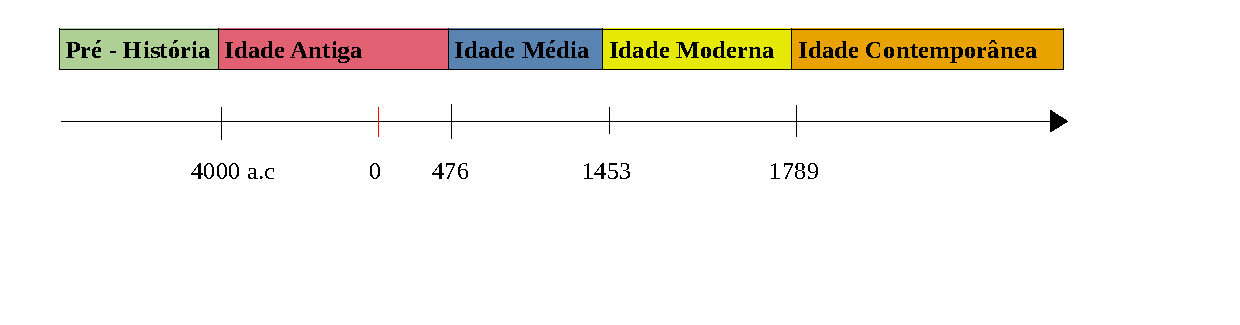
\includegraphics[width=\textwidth]{./cap_conjnum/figs/RetaCronologica}
 % \caption{Linha do tempo história geral}
 % \end{figure}

 % \begin{figure}[H]
 % \centering
 % 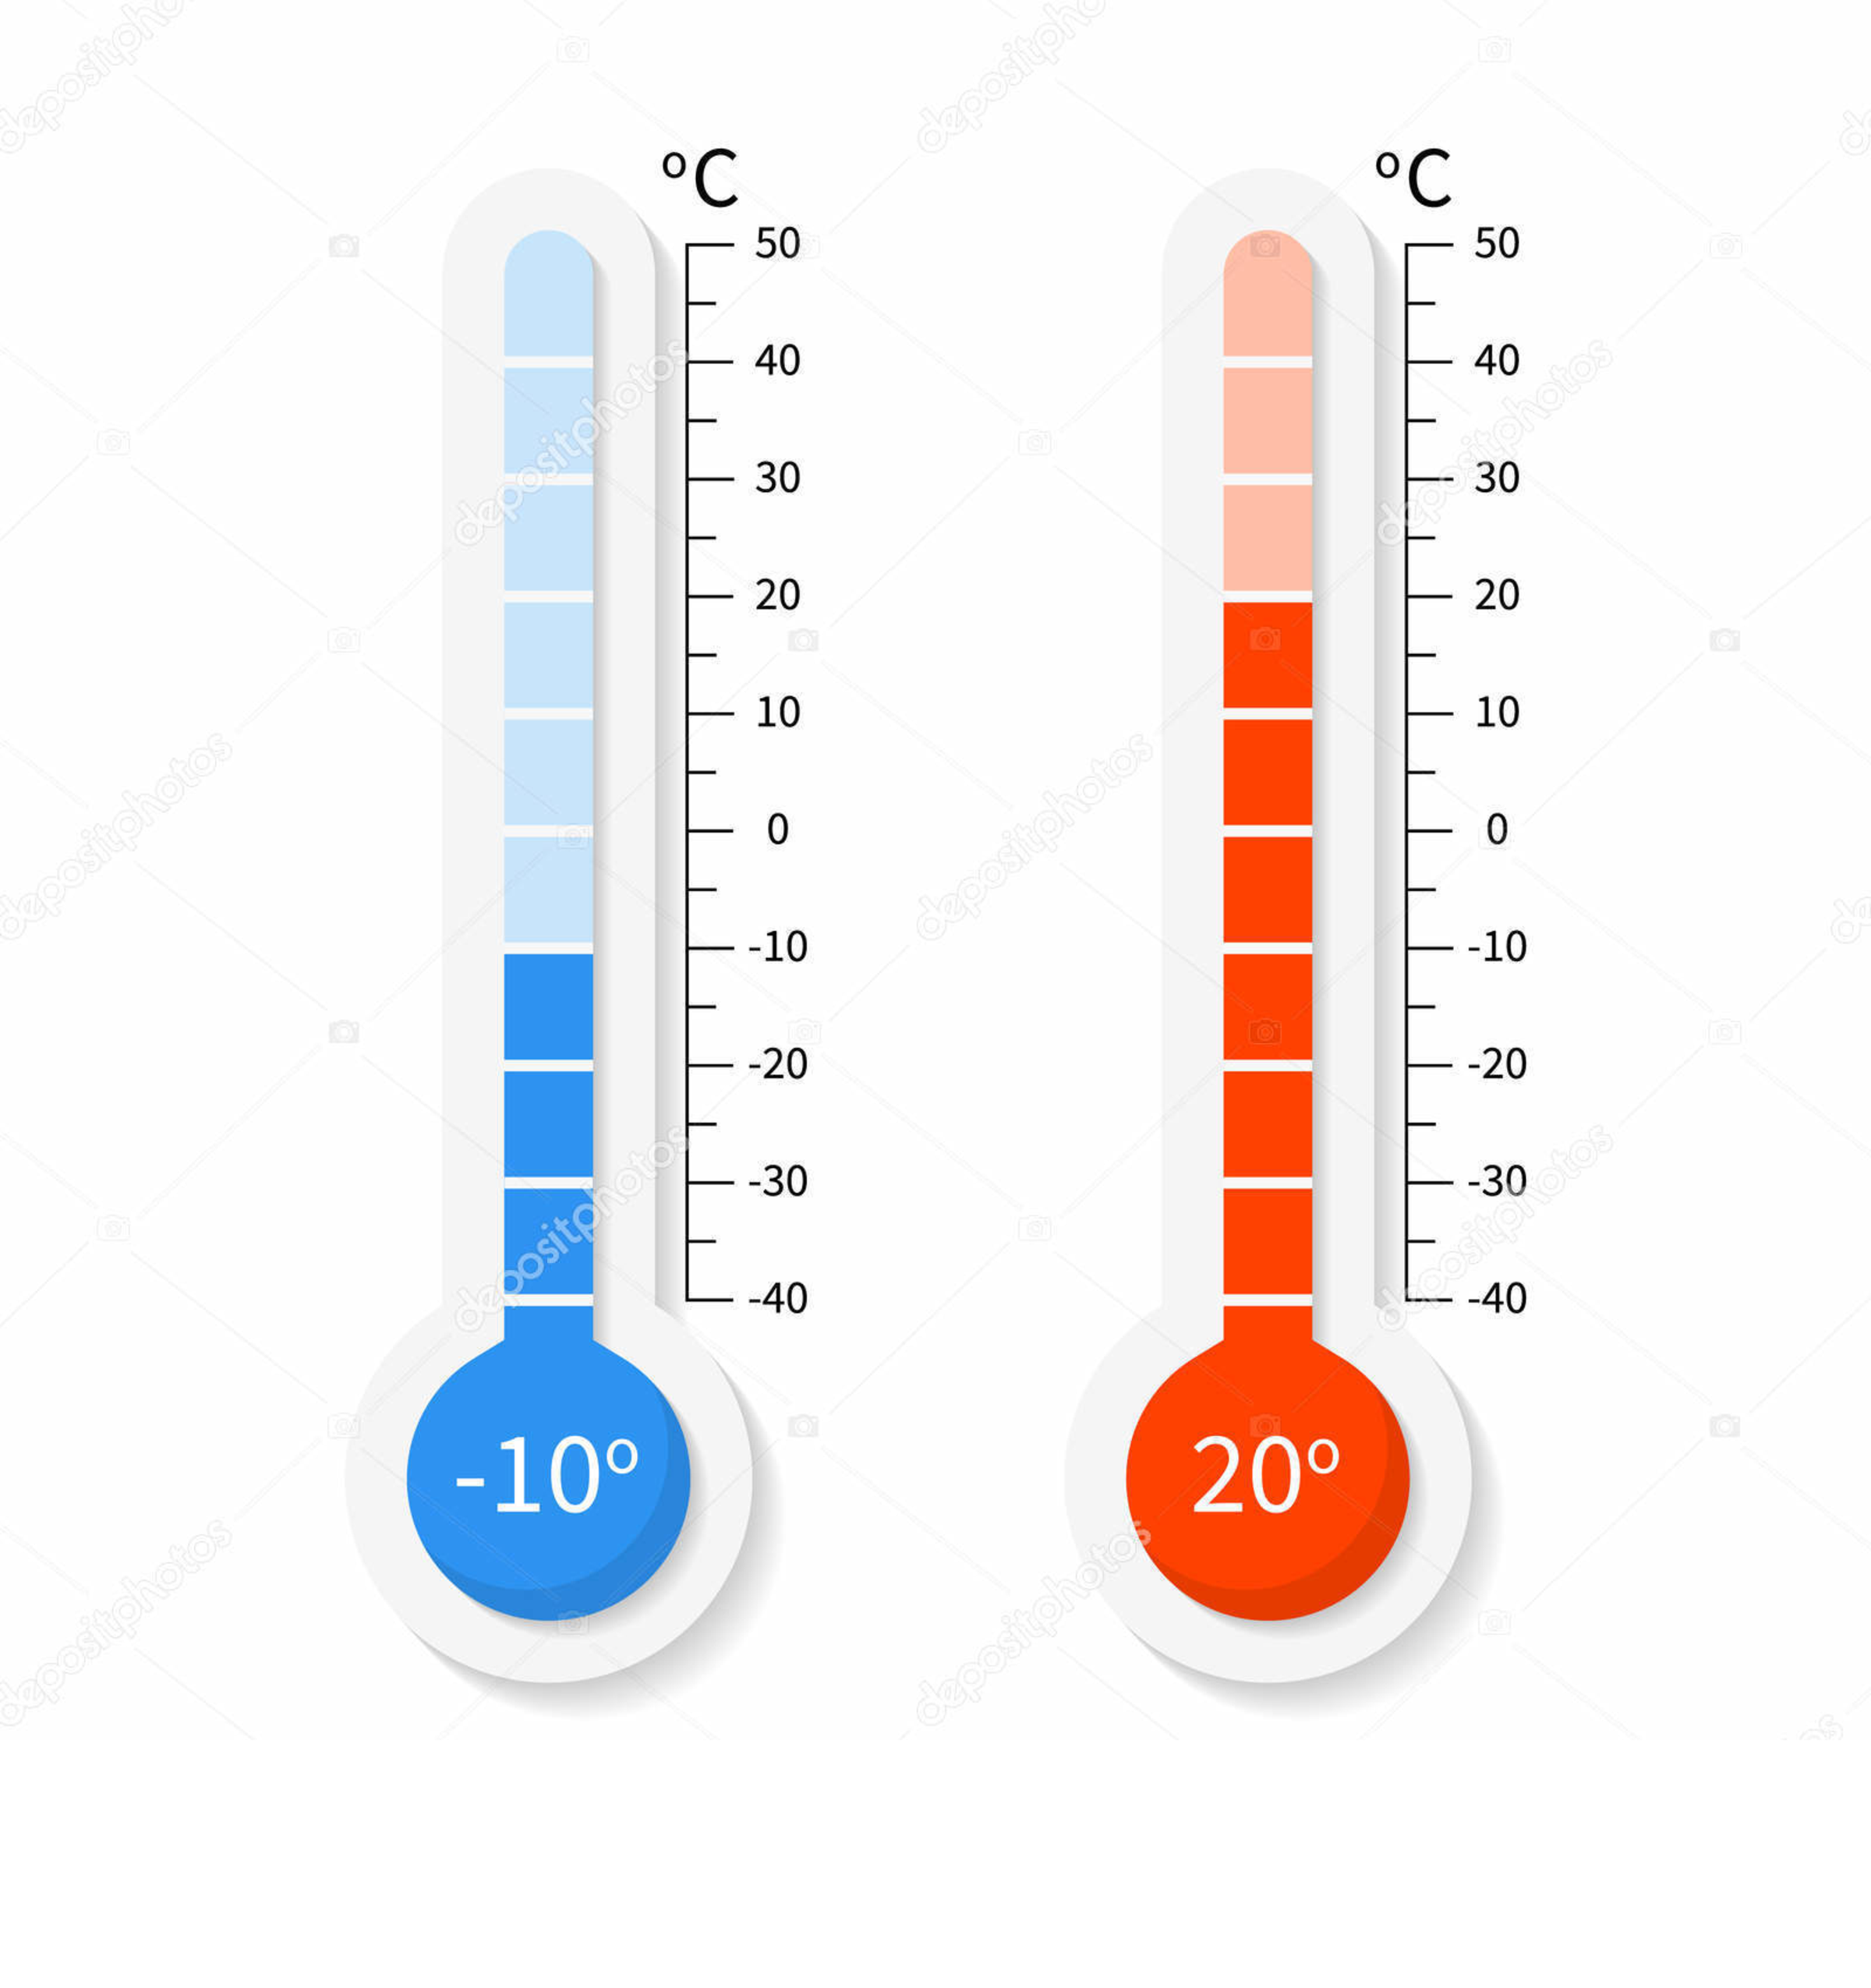
\includegraphics[width=6cm]{./cap_conjnum/figs/Termometro}
 % \caption{Termômetros apresentando a temperatura em graus Celsius}
 % \end{figure}

 Na reta real, o número $0$ (zero) serve como referência, sendo denominado origem. Os números positivos são representados à direita da origem e os números negativos à esquerda. Uma vez escolhida uma unidade de medida, exemplo centímetro, o número positivo $x$ é representado a exatamente $x$ unidade à direita do zero e o número $-x$ é representado a exatamente $x$ unidades à esquerda no zero.

\begin{center}
    \realline{-5}{5}[3][$x$][-3][$-x$]
\end{center}

 %  \begin{figure}[H]
 % \centering
 % 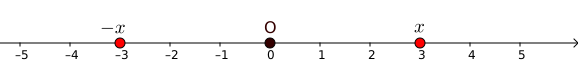
\includegraphics[width=\textwidth]{./cap_conjnum/figs/RetaReal}
 % \caption{Reta Real}
 % \end{figure}

%  Na reta real da figura acima intuitivamente observarmos que a distância dos pontos $-x$ e $x$ até a origem (zero) é de exatamente três unidades, esta distância de um ponto $x$ da reta real à origem é denominada \textbf{valor absoluto}\index{Valor absoluto|see{Módulo}}\index{Módulo}, ou \textbf{módulo}, do número $x$, e é representada por $\abs{x}$. Assim, dizemos que:
% \begin{itemize}
% \item O valor absoluto de $-3$ é $3$, ou seja, $\abs{-3}= 3$;
% \item O valor absoluto de $3$ é $3$, ou seja, $\abs{3}= 3$;
% \end{itemize}
% \begin{obs}
% Generalizando esta ideia temos pela definição que:
% \begin{equation*}
% \abs{x}= \begin{cases}
%       -x \ \ \text{se} \ \ x<0 \\
%       x \ \ \text{se} \ \ x \geq 0.
%      \end{cases}
% \end{equation*}
% \end{obs}

% O valor absoluto ou módulo de um número real conta com as seguintes propridades.

% \begin{prop}[Propriedades do módulo]
%  Para quaisquer $x, y \in \R$, são válidas as seguintes propriedades: \label{prop.modulo}
% \begin{enumerate}
%  \item $\abs{x} \geq 0$;
%  \item $\abs{x}= 0 \Leftrightarrow x= 0$;
%  \item $x \leq \abs{x}$;
%  \item $-x \leq \abs{x}$;
%  \item $\abs{-x}= \abs{x}$;
%  \item $\abs{x}^2= x^2$;
%  %, de fato,\\
%  %se $x \geq 0$, pela definição do módulo temos que $\abs{x}= x$ e daí $\abs{x}^2= x^2$, \\
%  %se $x < 0$, pela definição do módulo temos que $\abs{x}= -x$ e daí $\abs{x}^2=(-x)^2= x^2$.\\
%  %Portanto, para todo $x \in \R$, $\abs{x}^2= x^2$.

%  \item $\abs{x^n}= \abs{x}^n$, se $n$ é par;%, de fato, \\
%  %se $x \geq 0$, pela definição do módulo temos que $\abs{x}= x$ e daí $\abs{x}^n= x^n$, \\
%  %se $x < 0$, pela definição do módulo temos que $\abs{x}= -x$ e daí $\abs{x}^n= (-x)^n= x^n$.\\
%  %Portanto, para todo $x \in \R$, $\abs{x}^n= x^n$.

%  \item $\abs{x \cdot y}= \abs{x} \cdot \abs{y}$;%, de fato,
% %\begin{equation*}
% %\abs{x \cdot y}^2= (x \cdot y)^2= x^2 \cdot y^2= \abs{x}^2 \cdot \abs{y}^2= (\abs{x} \cdot \abs{y})^2 \ .
% %\end{equation*}
%  %Como $\abs{x \cdot y} \geqslant 0$ e $\abs{x} \cdot \abs{y} \geqslant 0$ resulta
% %\begin{equation*}
% %\abs{x \cdot y}= \abs{x} \cdot \abs{y} \ . 
% %\end{equation*}

%  \item $\abs{\dfrac{x}{y}}= \dfrac{\abs{x}}{\abs{y}}$, para $y \neq 0$;%, de fato,
% %\begin{equation*}
% %\abs{\dfrac{x}{y}}^2= \left(\dfrac{x}{y} \right)^2= \dfrac{x^2}{y^2}= \dfrac{\abs{x}^2}{\abs{y}^2}= \left( \dfrac{\abs{x}}{\abs{y}} \right)^2 \ . 
% %\end{equation*}
% % Como $\abs{\dfrac{x}{y}} \geq 0$ e $\dfrac{\abs{x}}{\abs{y}} \geq 0$ resulta que
% %\begin{equation*}
% %\abs{\dfrac{x}{y}}= \dfrac{\abs{x}}{\abs{y}} \ .
% %\end{equation*}

%  \item \emph{Desigualdade triangular:} $\abs{x+y}\leq \abs{x}+\abs{y}$;%, de fato, \\
%  %se $x + y \geqslant 0$, pela definição de módulo, $\abs{x+y}= x+y \leq \abs{x} + \abs{y}$; \\
%  %se $x + y < 0$, pela definição de módulo, $\abs{x+y}= -(x+y)= -x-y \leq \abs{x} + \abs{y}$. \\
%  %Logo, para quaisquer $x, y \in \R$ temos que
% %\begin{equation*}
% %\abs{x+y} \leq \abs{x}+\abs{y} \ .
% %\end{equation*}

%  \item $\abs{x-y} \leq \abs{x} + \abs{y}$;%, de fato \\
%  %Note que $x-y= x+ (-y)$, logo $\abs{x-y}= \abs{x+ (-y)}$ aplicando a desigualdade trinagular temos,
% %\begin{equation*}
% %\abs{x-y}= \abs{x+ (-y)} \leq \abs{x} + \abs{-y}= \abs{x} + \abs{y} \ .
% %\end{equation*}

%  \item $\abs{\abs{x} - \abs{y}} \leq \abs{x - y}$%, para mostrar esta desigualdade vamos fazer por partes.
%  %\begin{itemize}
%  %\item $\abs{x} - \abs{y} \leq \abs{x - y}$, \\
%  %de fato, pela desigualdade triangular temos que
% %\begin{equation*}
% %\abs{z+y} \leq \abs{z} + \abs{y}
% %\end{equation*}
% % subtraíndo $\abs{y}$ a ambos os termos temos,
% %\begin{equation*}
% %\abs{z+y} - \abs{y} \leq \abs{z}
% %\end{equation*}
% % fazendo $x= z+y$ temos que $z=x-y$ substituindo estes valores na equação acima obtemos
% %\begin{equation*}
% %\abs{x} - \abs{y} \leq \abs{x-y} \ . 
% %\end{equation*}
%  \item $\abs{y} - \abs{x} \leq \abs{x - y}$.%, \\
%  %de fato, pela desigualdade triangular temos que
% %\begin{equation*}
% %\abs{x+z} \leq \abs{x} + \abs{z}
% %\end{equation*}
% % subtraíndo $\abs{x}$ a ambos os termos temos,
% %\begin{equation*}
% %\abs{x+z} - \abs{x} \leq \abs{z}
% %\end{equation*}
%  %fazendo $y= x+z$ temos que $z=y-x$ substituindo estes valores na equação acima obtemos
% %\begin{equation*}
% %\abs{y} - \abs{x} \leq \abs{y-x}= \abs{x-y} \ . 
% %\end{equation*}
% %\end{itemize}

% % Portanto,
% %\begin{equation*}
% % \abs{\abs{x} - \abs{y}} = \pm (\abs{x} - \abs{y}) \leq \abs{x-y} \ .
% %\end{equation*}

% \end{enumerate}
% \end{prop}

% \subsection{Operações nos reais}
% Dados quaisquer $x, y, z \in \R$, destacamos que em $\R$ as operações de soma (adição) $(+)$ e multiplicação $(\cdot)$ possuem as seguintes propriedades:

% \begin{obs}
%  Adição $(+)$:
%  \begin{enumerate}[1)]
%  \item Fechamento: $x+y \in \R$;
%  \item Associativo: $(x+y)+z= x+(y+z)$;
%  \item Elemento neutro: existe um elemento $0 \in \R$ tal que $x+0=0+x=x$;
%  \item Elemento inverso: existe um elemento $-x \in \R$ tal que $x+(-x)=0$;
%  \item Comutatividade: $x+y= y+x$.
%  \end{enumerate}
% \end{obs}

% \begin{obs}
%   Multiplicação $(\cdot)$:
%  \begin{enumerate}[1)]
%  \item Fechamento: $x \cdot y \in \R$;
%  \item Associativo: $(x \cdot y) \cdot z= x \cdot (y \cdot z)$;
%  \item Elemento neutro: existe um elemento $1 \in \R$ tal que $x \cdot 1= 1 \cdot x= x$;
%  \item Elemento inverso: existe um elemento $x^{-1} \in \R$ tal que $x \cdot x^{-1}= 1$;
%  \item Comutatividade: $x \cdot y= y \cdot x$.
%  \end{enumerate}
% \end{obs}

% \begin{obs}
%   Leis distributivas: 
%  \begin{enumerate}[1)]
%  \item $x \cdot (y + z)= x \cdot y + x \cdot z$;
%  \item $(x + y) \cdot z= x \cdot z + y \cdot z$.
%  \end{enumerate}
% \end{obs}

%    As operações de soma e produto no conjunto dos números reais satisfazem também a:
%    \begin{itemize}
%    \item \textit{Lei do cancelamento:} Para todos $x, y, z \in \R$  temos que
% \begin{equation*}
% x+z=y+z \ \ \ \Rightarrow \ \ \ x=y  . 
% \end{equation*}
%    \item \textit{Anulamento do produto:} Para todos $x, y \in \R$  temos que
% \begin{equation*}
% x \cdot y= 0 \Leftrightarrow x=0 \ \ \ \text{ ou } \ \ \ y=0 \ .
% \end{equation*}
%    \end{itemize}

\section{Conjunto dos números Complexos}

Apesar de nossos estudos neste curso ser focado no conjunto dos números reais, neste conjunto numérico não conseguimos resolver todos os problemas matemáticos, em virtude disso, temos por exemplo o conjunto do números complexos, quatérnios, entre outros, desses mais avançados vamos falar um pouquinho dos números complexos pois neste conjunto é possível calcular raiz quadrada de qualquer número, o que não ocorre nos reais.

Para resolver o problema da raiz quadrada de um número negativo, criou-se o número imaginário puro $i$, definido por $\iu= \sqrt{-1}$, portanto $\iu^2= -1$, criou-se assim um número $\iu$ que elevado ao quadrado desse $-1$. Temos agora como calcular a raiz quadrada de qualquer número real. Definimos a partir deste número imaginário o conjunto dos números complexos por:
\begin{equation*}
\C= \{a + b\iu \mid a, b \in \R \} ,
\end{equation*}
cujas operações apresentam algumas particularidades e portanto trataremos delas mais adiante.

Note que, se tivermos $b=0$, estamos com o conjunto dos números reais, portanto $\R \subset \C$. Para fixar a ordem de continência destes conjuntos numéricos, observemos o diagrama de Venn abaixo.

 \begin{figure}[H]
    \centering
    \begin{tikzpicture}[scale=0.7]
    \draw[fill=blue!30] (2,0) ellipse (5cm and 2.5cm);
    \draw[fill=green!30] (1.5,0) ellipse (4cm and 2cm);
    \draw[fill=yellow!30] (1,0) ellipse (3cm and 1.5cm);
    \draw[fill=orange!30] (0.5,0) ellipse (2cm and 1cm);
    \draw[fill=red!30] (0,0) ellipse (1cm and 0.5cm);   
    \draw (-0.05,0) node{$\mathbb{N}$};
    \draw (1.5,0.2) node{$\mathbb{Z}$};
    \draw (3.0,0.4) node{$\mathbb{Q}$};
    \draw (4.5,0.6) node{$\mathbb{R}$};
    \draw (6,0.8) node{$\mathbb{C}$};
    \end{tikzpicture}
    \caption{Representação conjuntos numéricos}
  \end{figure}

\section{Subconjuntos numéricos e suas representações}

Um tipo importante de subconjuntos de $\R$ são os \emph{intervalos}, que são determinados por desigualdades.

%\textbf{Intervalos numéricos limitados}\index{Intervalos numéricos!limitados}
\begin{itemize}
 \item Intervalo aberto: $(a, b)= \{x \in \R \mid a < x < b\}$:
 \begin{center}
     \intervalo{11}{$a$}{$b$}
 \end{center}

 A bolinha aberta $\circ$ indica que os extremos não pertencem ao intervalo.

 \item Intervalo fechado: $[a, b]= \{x \in \R \mid a \leq x \leq b\}$:
 \begin{center}
     \intervalo{22}{$a$}{$b$}
 \end{center}

  A bolinha fechada $\bullet$ indica que os extremos pertencem ao intervalo.
 \item Intervalo aberto à direita e fechado à esquerda: $[a, b)= \{x \in \R \mid a \leq x < b\}$:
 \begin{center}
     \intervalo{21}{$a$}{$b$}
 \end{center}
 \item Intervalo aberto à esquerda e fechado à direita: $(a, b]= \{x \in \R \mid a < x \leq b\}$:
 \begin{center}
     \intervalo{12}{$a$}{$b$}
 \end{center}
%\end{itemize}

%\textbf{Intervalos numéricos ilimitados}\index{Intervalos numéricos!ilimitados}
%\begin{itemize}
\item Conjunto dos números reais maiores que $a$: $(a, +\infty) = \{ x \in \R \mid a < x \}$:
  \begin{center}
     \intervalo{10}{$a$}{$b$}
 \end{center}

\item Conjunto dos números reais maiores ou iguais à $a$: $[a, +\infty) = \{ x \in \R \mid a \leq x \}$:
 \begin{center}
     \intervalo{20}{$a$}{$b$}
 \end{center}

\item Conjunto dos números reais menores que $b$: $(-\infty, b) = \{ x \in \R \mid x < b \}$:
 \begin{center}
     \intervalo{01}{$b$}{$b$}
 \end{center}

\item Conjunto dos números reais menores ou iguais à $b$: $(-\infty, b] = \{ x \in \R \mid x \leq b \}$:
 \begin{center}
     \intervalo{02}{$b$}{$b$}
 \end{center}
% \item Conjunto dos números reais: $(-\infty, +\infty) = \R$
%  \begin{figure}[H]
%  \centering
%  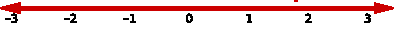
\includegraphics[width=7.5cm]{./cap_conjnum/figs/reta}
%  \end{figure}
\end{itemize}

O conjunto dos números reais pode ser denotado como $(-\infty, +\infty) = \R$.


% \textbf{Outros subconjuntos dos números reais}
% \begin{itemize}
%  \item Conjunto dos números reais não-nulos: $\R^{*}=\{x \in \R \mid x \neq 0\}$;
%  \begin{figure}[H]
%  \centering
%  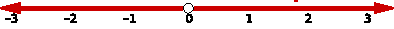
\includegraphics[width=7.5cm]{./cap_conjnum/figs/n-nulos}
%  \end{figure}
%  \item Conjunto dos números reais não-negativos: $\R_{+}=\{x \in \R \mid x \geq 0\}$;
%  \begin{figure}[H]
%  \centering
%  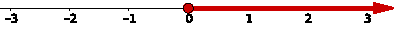
\includegraphics[width=7.5cm]{./cap_conjnum/figs/n-negativos}
%  \end{figure}
%  \item Conjunto dos números reais positivos: $\R^{*}_{+}=\{x \in \R \mid x > 0\}$;
%  \begin{figure}[H]
%  \centering
%  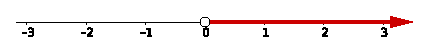
\includegraphics[width=7.5cm]{./cap_conjnum/figs/positivos}
%  \end{figure}
%  \item Conjunto dos números reais não-positivos: $\R_{-}=\{x \in \R \mid x \leq 0\}$;
%  \begin{figure}[H]
%  \centering
%  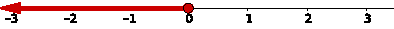
\includegraphics[width=7.5cm]{./cap_conjnum/figs/n-positivos}
%  \end{figure}
%  \item Conjunto dos números reais negativos: $\R^{*}_{-}=\{x \in \R \mid x < 0\}$.
%  \begin{figure}[H]
%  \centering
%  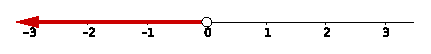
\includegraphics[width=7.5cm]{./cap_conjnum/figs/negativos}
%  \end{figure}
% \end{itemize}

\begin{obs}
    No Ensino Médio, costumamos denotar um intervalo aberto por $]a,b[$. No Cálculo, os autores frequentemente utilizam a notação $(a,b)$ introduzida neste texto. Nesta notação, é importante ficar atento ao contexto, pois ela coincide com a notação de par ordenado.
\end{obs}

\section{Operações com conjuntos numéricos}

 Podemos realizar as operações de união, interseção, diferença e produto cartesiano entre conjuntos no contexto de subconjuntos dos números reais. A atenção especial a este tipo de conjunto se deve a extensa utilização destas operações para determinar o conjunto solução de equação e inequações, bem como para determinar o domínio de algumas funções, temas centrais deste curso.

\begin{exem}
    Sejam $A=(-2,6)$ e $B=[\frac{3}{2},8)$. A interseção entre os intervalos pode ser representada pelo ``varal'' de interseção:
    \begin{intervaloper}[3]{-3}{9}
        \linelabel{1}{$A$}
        \linelabel{2}{$B$}
        \linelabel{3}{$A\cap B$}
        \dashes{6}{1}{3}
        \dashes{3/2}{1}{3}
        \interval{1}{11}{-2,6}
        \interval{2}{21}{3/2,8}
        \intervalcolor{blue}
        \interval{3}{21}{3/2,6}
    \end{intervaloper}

    Logo, $A\cap B=[\frac{3}{2},6)$.
\end{exem}

\begin{exem}
    Sejam $A=(-\infty,1]$ e $B=(-2,4)$. A diferença $A-B$  pode ser representada por:
    \begin{intervaloper}[3]{-3}{5}
        \linelabel{1}{$A$}
        \linelabel{2}{$B$}
        \linelabel{3}{$A-B$}
        \dashes{-1}{1}{3}
        %\dashes{3/2}{1}{3}
        \interval{1}{01}{1}
        \interval{2}{11}{-1,4}
        \intervalcolor{blue}
        \interval{3}{02}{-1}
    \end{intervaloper}

    Logo, $A-B=(-\infty, -1]$.
\end{exem}

\begin{exem}
    Dado $A=[3,6)$, o seu complementar $A^C$ é igual à diferença $\R-A$. 
    \begin{intervaloper}[2]{1.5}{7.5}
        \linelabel{1}{$A$}
        \linelabel{2}{$A^C$}
        \dashes{3}{1}{2}
        \dashes{6}{1}{2}
        \interval{1}{21}{3,6}
        \intervalcolor{blue}
        \interval{2}{01}{3}
        \interval{2}{20}{6}
    \end{intervaloper}

    Logo, $A^C=(-\infty,3)\cup [6,\infty)$.
\end{exem}

Para entender melhor como as operações de união, interseção e diferença entre intervalos de maneira interativa, veja o seguinte material do Geogebra:

\geogebra{https://www.geogebra.org/m/kjf4tycp}{Operações com intervalos reais}

% Vamos agora apresentar alguns exemplos de como aplicar as operações de união, interseção, diferença e produto cartesiano entre conjuntos no contexto de subconjuntos dos números reais. A atenção especial a este tipo de conjunto se deve a extensa utilização destas operações para determinar o conjunto solução de equação e inequações, bem como para determinar o domínio de algumas funções, temas centrais deste curso.

% \begin{itemize}
%  \item Caso $a< b< c< d$ temos que $[a, b] \cup [c, d]$ pode ser representado por:
%   \begin{figure}[H]
%  \centering
%  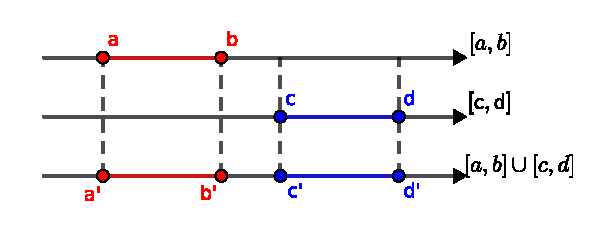
\includegraphics[width=8cm]{./cap_conjnum/figs/uniaoabcd}
%  \end{figure}

%  \item Caso $a< c< b< d$ temos que $[a, b] \cup [c, d]= [a, d]$ pode ser representado por:
%   \begin{figure}[H]
%  \centering
%  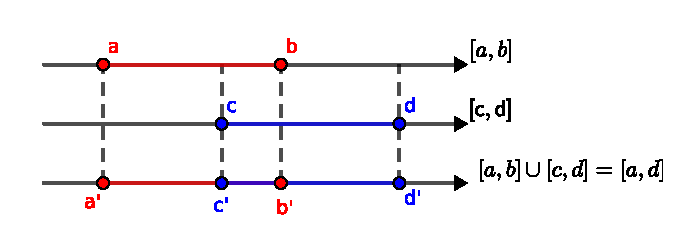
\includegraphics[width=8cm]{./cap_conjnum/figs/uniaoacbd}
%  \end{figure}

%   \item Caso $a< c< d< b$ temos que $[a, b] \cup [c, d]= [a, b]$ pode ser representado por:
%   \begin{figure}[H]
%  \centering
%  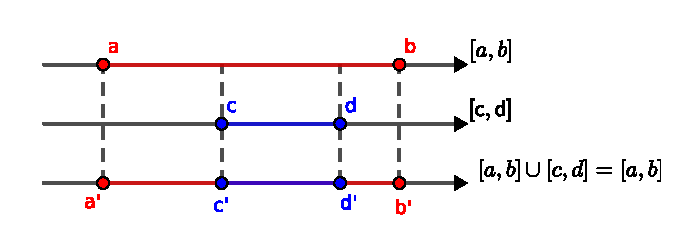
\includegraphics[width=8cm]{./cap_conjnum/figs/uniaoacdb}
%  \end{figure}

%  %%%%%%%%%%%%%%%%%%%%
%  \item Caso $a< b< c< d$ temos que $[a, b] \cap [c, d]= \varnothing$ pode ser representado por:
%   \begin{figure}[H]
%  \centering
%  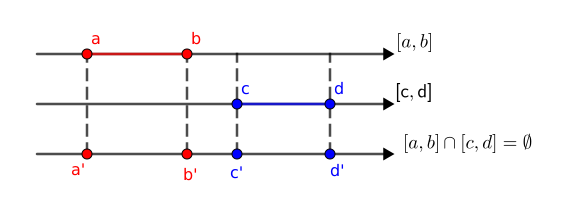
\includegraphics[width=8cm]{./cap_conjnum/figs/intersecaoabcd}
%  \end{figure}

%  \item Caso $a< c< b< d$ temos que $[a, b] \cap [c, d]= [c, b]$ pode ser representado por:
%   \begin{figure}[H]
%  \centering
%  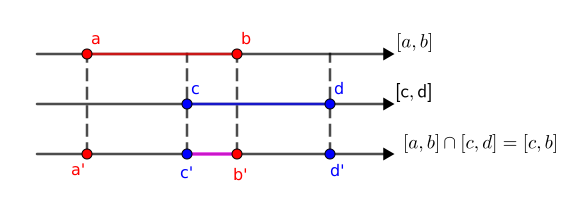
\includegraphics[width=8cm]{./cap_conjnum/figs/intersecaoacbd}
%  \end{figure}

%   \item Caso $a< c< d< b$ temos que $[a, b] \cap [c, d]= [c, d]$ pode ser representado por:
%   \begin{figure}[H]
%  \centering
%  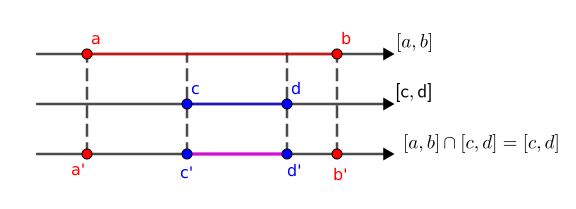
\includegraphics[width=8cm]{./cap_conjnum/figs/intersecaoacdb}
%  \end{figure}

% \end{itemize}

% \begin{obs}
% Os exemplos acima foram apresentados apenas utilizando intervalos fechados. No entanto, é possível combinar com intervalos aberto em algum dos lados ou ambos.
% \end{obs}

% \begin{itemize}
%  \item Considere agora o conjunto $A= [1, \infty) \times [2, 4)$, que é também representado da seguinte forma:
% \begin{equation*}
% A= \{(x, y) \in \R^2 \mid 1 \leq x \text{ e } 2 \leq y < 4 \}
% \end{equation*}
%    \begin{figure}[H]
%  \centering
%  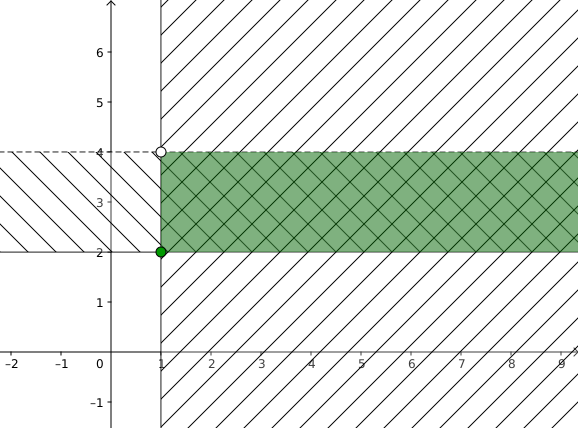
\includegraphics[width=8cm]{./cap_conjnum/figs/cartesiano1infty24}
%  \end{figure}

%  \item Considere agora o conjunto $B= [1, 4) \times [3, 5)$, que é também representado da seguinte forma:
% \begin{equation*}
% B= \{(x, y) \in \R^2 \mid 1 \leq x \leq 4 \text{ e } 3 \leq y < 5 \}
% \end{equation*}
%    \begin{figure}[H]
%  \centering
%  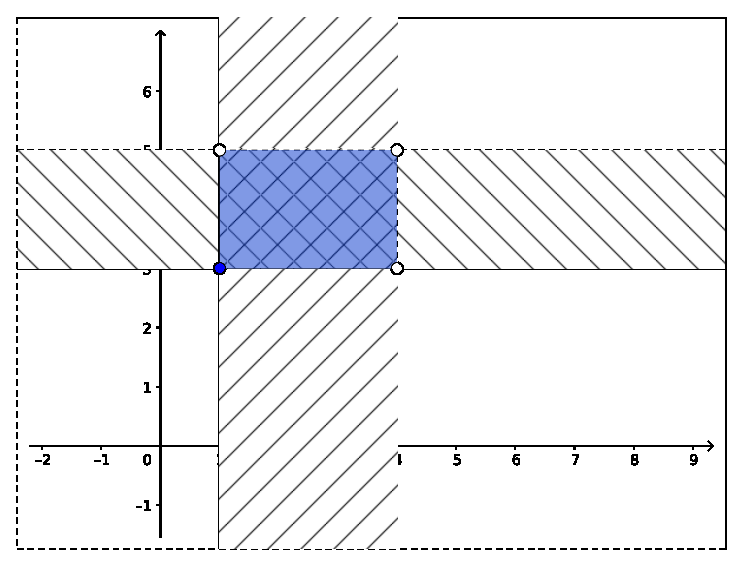
\includegraphics[width=8cm]{./cap_conjnum/figs/cartesiano1435}
%  \end{figure}

%  \item Considerando agora os seguintes conjuntos $A$ e $B$:
% \begin{gather*}
% A= \{(x, y) \in \R^2 \mid 1 \leq x \text{ e } 2 \leq y < 4 \}\\
% B= \{(x, y) \in \R^2 \mid 1 \leq x \leq 4 \text{ e } 3 \leq y < 5 \}
% \end{gather*}
%  temos que:

%  \begin{itemize}
%  \item $A \cap B$ é representado graficamente por:
%     \begin{figure}[H]
%  \centering
%  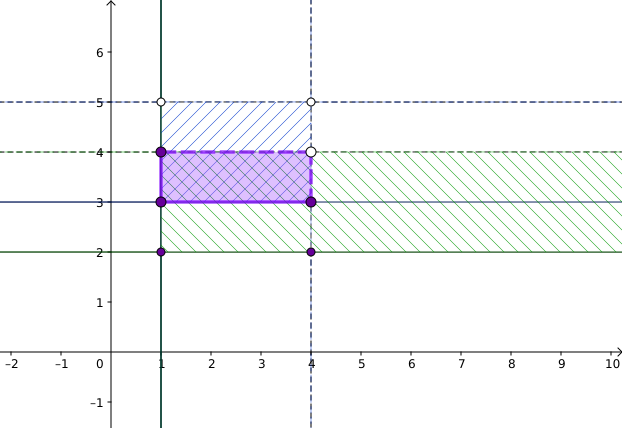
\includegraphics[width=8cm]{./cap_conjnum/figs/cartesianointersecao}
%  \end{figure}
%  \item $A \cup B$ é representado graficamente por:
%     \begin{figure}[H]
%  \centering
%  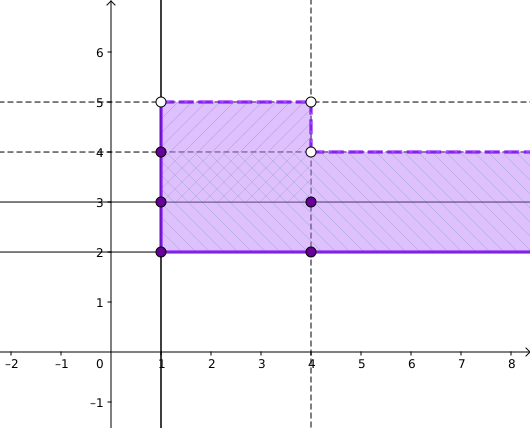
\includegraphics[width=8cm]{./cap_conjnum/figs/cartesianouniao}
%  \end{figure}

%  \end{itemize}

% \end{itemize}

\video{https://www.youtube.com/watch?v=etpDR-8mn9s}{Outras coisas interessantes sobre os conjuntos númericos.}

\newpage

\begin{secExercicios}

\begin{exer}
    Efetue as operações entre os intervalos:
    \begin{multicols}{2}
    \begin{enumerate}[a)]
        \item $(1,2]\cup [2,3)$
        \item $(1,5)\cup (4,10)$
        \item $[10,15]\cup[5,8]$
        \item $(1,2]\cap [2,3)$
        \item $[0,1)\cap (1,2]$
        \item $[10,15]\cap[5,8]$
        \item $(-\infty,2)\cup [2,3)$
        \item $(1,3)\cap (2,\infty)$
    \end{enumerate}
    \end{multicols}
\end{exer}

\begin{exer}
    Represente os conjuntos sob a forma de intervalo
    \begin{enumerate}[a)]
        \item $\{x\in\R\colon 1<x<2\}$
        \item $\{x\in\R\colon -3<x\leqslant 4\}$
        \item $\{x\in\R\colon x>-5\}$
        \item $\{x\in\R\colon x\leqslant 9\}$
        \item $\{x\in\R\colon x<2 \mbox{ ou } x\geqslant 3\}$
    \end{enumerate}
\end{exer}

\begin{exer}
    Dados $A=\{x\in\R \colon -4 < x \leqslant 3\}$, $B=[-3,5]$ e $C=(-\infty, 1)$, determine e represente na reta real:
    \begin{enumerate}[a)]
    \begin{multicols}{2}
        \item $A\cap B$;
        \item $A\cup C$;
        \item $A^c$;
        \item $A\cap C^c$;
        \item $(A\cup B)\cap C$;
        \item $(A\cap C)-C$.
    \end{multicols}
    \end{enumerate}
\end{exer}

\begin{exer}
    Usando notação de conjuntos, escreva os intervalos:
    \begin{multicols}{2}
        \begin{enumerate}[a)]
            \item $[3,5)$
            \item $(-\infty,4)$
            \item $(-5,2]$
            \item $[0,\infty)$
        \end{enumerate}
    \end{multicols}
\end{exer}

\begin{exer}
    Represente os intervalos do exercício anterior na reta real.
\end{exer}

\begin{exer}
    Dê um exemplo de um intervalo aberto e um intervalo fechado cuja união é igual ao intervalo $(1,4)$.
\end{exer}

\begin{exer}
    Dê um exemplo de um intervalo aberto e um intervalo fechado cuja interseção é igual ao intervalo $[-3,5]$.
\end{exer}

\begin{exer}
    Sendo o conjunto $A = \{x\in \Z \colon -5 < x < -2\}$ e $B = \{x\in \Z \colon - 3 < x < 0\}$, represente os intervalos de $A$ e $B$ e faça a união dos dois conjuntos.
\end{exer}

\begin{exer}
    Determine se as sentenças são verdadeiras ou falsas.
    \begin{enumerate}[a)]
        \item O conjunto dos números naturais é finito.
        \item A soma de dois números irracionais pode ser um número irracional.
        \item A soma de dois números irracionais é sempre um número irracional.
        \item o produto de dois números irracionais pode ser um número racional.
        \item o produto de dois números irracionais é sempre um número racional.
    \end{enumerate}
\end{exer}
\begin{resp}
    a) F; b) V; c) F; d) V; e) F
\end{resp}

\begin{exer}
    Determine o número racional $\frac{p}{q}$, com $p,q$ inteiros, que gera as dízimas periódicas a seguir:
    \begin{multicols}{2}
    \begin{enumerate}[a)]
        \item $0,141414\dots$
        \item $4,3333\dots$
        \item $2,181818\dots$
        \item $7,38282\dots$
    \end{enumerate}
    \end{multicols}
\end{exer}

\begin{exer}
    Qual o valor da soma $1,3333\dots + 0,16666\dots$?
\end{exer}

\begin{exer}
    Escreva o número $x =\sqrt{13,4444\dots}$ como uma fraçãao de números inteiros.
\end{exer}
% \begin{resp}
%     \par\noindent\rule{\columnwidth}{0.4pt}
% \end{resp}

%\subsection*{Respostas:}
%\noindent{\footnotesize \textit{*Em elaboração}}

%\shipoutAnswer

\end{secExercicios}
%%Este trabalho está licenciado sob a Licença Creative Commons Atribuição-CompartilhaIgual 4.0 Internacional. Para ver uma cópia desta licença, visite https://creativecommons.org/licenses/by-sa/4.0/ ou envie uma carta para Creative Commons, PO Box 1866, Mountain View, CA 94042, USA.

\markboth{\sffamily\normalsize\bfseries Respostas dos Exercícios}{\sffamily\normalsize\bfseries Respostas dos Exercícios} % Set the page headers to display a Bibliography chapter name
\addcontentsline{toc}{chapter}{\textcolor{ocre}{Respostas dos Exercícios}}
\chapter*{Respostas dos Exercícios}
%\addcontentsline{toc}{Part}{Respostas dos Exercícios}
%\fancyhead[RE]{Introdução à Matemática Superior}
%\fancyhead[LO]{RESPOSTAS DOS EXERCÍCIOS}
%\fancyhead[LE,RO]{\thepage}

Devido a construção deste material, muitas respostas ainda não foram incluídas, podem conter imprecisões e erros.

\setlength{\columnseprule}{1pt}

\begin{multicols}{2}
\shipoutAnswer
\end{multicols}

\setlength{\columnseprule}{0pt}


%

% \setcounter{part}{1}
\part{Equações e Inequações}
%\setcounter{chapter}{4} 
%Este trabalho está licenciado sob a Licença Creative Commons Atribuição-CompartilhaIgual 4.0 Internacional. Para ver uma cópia desta licença, visite https://creativecommons.org/licenses/by-sa/4.0/ ou envie uma carta para Creative Commons, PO Box 1866, Mountain View, CA 94042, USA.

\chapter{Equações}
%\label{cap:0}

Uma equação é uma sentença matemática aberta, ou seja, sentença matemática que possui ao menos uma incógnita, e que estabelece uma igualdade entre duas expressões matemáticas.

 \begin{exem}
 A seguintes expressões matemáticas são exemplos de equações:

\begin{enumerate}[(1)]
 \item $x+1=3$;
 \item $\sin(x)=0$;
 \item $x^2+3x+1=0$;
 \item $\ln(x)= 5$.
\end{enumerate}
\end{exem}

 E para ajudar a entender o conceito de equação, seguem algumas expressões matemáticas que não são equações, com a justificativa do porquê elas não são equações:
\begin{exem}
\begin{enumerate}[(1)]
 \item Uma desigualdade, ou seja, uma sentença matemática que relaciona duas expressões matemáticas através do sinal de diferente ($\neq$), não é uma equação, exemplo: $x+1 \neq 3$.

 \item $3 + 2 = 5$, por não ser uma sentença aberta.

 Sentenças matemáticas que relacionam duas expressões matemáticas através dos sinais de menor ($<$), maior ($>$), menor ou igual ($\leqq$), maior ou igual ($\geqq$), não são equações. Elas são chamadas de inequações. Seguem alguns exemplos:

 \item $\sin(x) < 0$, neste caso o sinal de menor $<$, nos diz que $\sin(x)$ é menor do que $0$.
 \item $2x+3 \leqq 7x-2$.
 \item $x^2+3x+1 \geqq 0$.
\end{enumerate}
\end{exem}

% Vamos nos dedicar nesta seção para entender as equações de 1º grau e as de 2º grau. Mas antes vejamos um exemplo de como as equações aparecem em nosso dia-a-dia.

% \begin{exem}
%  Situação problema: Geraldo frequenta uma lan house, pois não tem internet em sua casa, e paga uma taxa fixa de $R\$ 1,00$ a primeira hora, mais $R\$ 2,00$ a cada hora excedente. Se após o uso Geraldo pagou $R\$ 7,00$, por quanto tempo ele usou a internet?

%  \underline{Resolução:}

%  Podemos concluir que Geraldo usou o computador por $4$ horas, já que pagou $R\$ 1,00$ pela primeira hora, e consequentemente $(7,00 - 1,00 = 6,00)$ $R\$ 6,00$ pelas demais horas, como cada hora a mais custa $R\$ 2,00$ e $(6,00 \div 2,00 = 3)$ temos então que Geraldo usou $(1 + 3 = 4)$ horas.

%  Podemos generalizar esta situação usando a letra $x$ para representar o tempo de internet utilizado, que é o valor que não conhecemos, chegando à seguinte equação: $2x + 1 = 7$.
% \end{exem}

A equação resultante desta situação problema é o que chamamos de equação do 1º grau.

\section{Equações do 1º grau}

\begin{obs}
   As equações de 1º grau tem a seguinte forma geral:
\begin{equation*}
ax + b = 0
\end{equation*}
onde $a, b \in \mathbb{R}$ são números dados (conhecidos), com $a \neq 0 $.
\end{obs}

Como resolver uma equação destas, ou equivalentemente, como encontrar o valor de $x$:
\begin{equation*}
ax + b = 0 \Rightarrow ax= -b \Rightarrow x = \frac{-b}{a} .
\end{equation*}


\begin{exem}
 Resolva as seguintes equações do 1º grau:
 \begin{enumerate}[a)]
  \item $ax = 0$

  Neste caso $a \neq 0$, como produto de dois números só é zero quando um deles for igual a zero concluímos que $x = 0$.
  
  \item $2x + 4 = 0$
  \begin{equation*}
  2x + 4 = 0 \Rightarrow 2x = -4 \Rightarrow x = \frac{-4}{2} \Rightarrow x = -2
  \end{equation*}
  
  % \item $3x - 5 = 4$
  % \begin{equation*}
  % 3x - 5 = 4 \Rightarrow 3x = 4 +5 \Rightarrow 3x = 9 \Rightarrow x = \frac{9}{3} \Rightarrow x = 3
  % \end{equation*}
  
  \item $3(x + 2)= 12$
  \begin{equation*}
  3(x + 2)= 12 \Rightarrow 3x + 6 = 12 \Rightarrow 3x = 12 - 6 \Rightarrow 3x = 6 \Rightarrow x = \frac{6}{3} \Rightarrow x = 2
  \end{equation*}
  
  \item $\dfrac{-(3x+4)}{5}= x-2$
  \begin{eqnarray*}
  \dfrac{-(3x+4)}{5} &=& x-2 \\
   -3x-4 &=& 5(x-2) \\ 
   -3x-4 &=& 5x -10 \\
   -3x - 5x &=& -10 + 4 \\ 
   -8x &=& -6 \\ 
   x &=& \dfrac{-6}{-8} \\
   x &=& \dfrac{3}{4}
  \end{eqnarray*}
  
  \item $\dfrac{x}{4} + 5= \dfrac{23}{4}$
  \begin{equation*}
  \dfrac{x}{4} + 5= \dfrac{23}{4} \Rightarrow \dfrac{x + 20}{4}= \dfrac{23}{4} \Rightarrow x+20= 23 \Rightarrow x= 23-20 \Rightarrow x= 3
  \end{equation*}
 
  \end{enumerate}
\end{exem}

\section{Equações do 2º grau}

\begin{obs}
   As equações de 2º grau tem a seguinte forma geral:
\begin{equation*}
ax^2 + bx + c = 0
\end{equation*}
  onde $a, b, c \in \mathbb{R}$ são números dados (conhecidos), com $a \neq 0 $.
\end{obs}


Para resolver este tipo de equação usamos a fórmula da equação do 2º grau também conhecida como a \textbf{fórmula de Bhaskara}, dada por:
\begin{equation*}
  x= \frac{-b \pm \sqrt{b^2 - 4ac}}{2a}.
\end{equation*}

Lembremos que $z^2= (-z)^2$ e que extrair a raiz quadrada de um número $y$ é procurar o número $z$ tal que $z= -\sqrt{y}$ e $z= \sqrt{y}$ donde obtemos que $z= \pm \sqrt{y}$. Por isso precisamos colocar o sinal $(\pm)$ antes da raiz quadrada na equação acima.

A fórmula de Bhaskara é também reescrita da seguinte forma:
\begin{equation*}
x= \frac{-b \pm \sqrt{\Delta}}{2a} \ \ \ \text{ para } \ \ \ \Delta= b^2 - 4ac
\end{equation*}
onde $\Delta$ é chamado de discriminante.

A partir da análise do sinal do discriminante determinamos se as equações do 2º grau possuem $0$, $1$ ou $2$ soluções diferentes no conjunto dos números reais, da seguinte forma:
\begin{itemize}
\item Se $\Delta < 0$ a equação não possui raízes reais, pois em $\R$ não existe raíz quadrada de número negativo.
\item Se $\Delta = 0$ a equação possui apenas a solução $x= \frac{-b}{2a}$ (também dizemos que a equação tem duas soluções iguais).
\item Se $\Delta > 0$ a equação possui duas raízes reais distintas, $x_1= \frac{-b - \sqrt{\Delta}}{2a}$ e $x_2= \frac{-b + \sqrt{\Delta}}{2a}$.
\end{itemize}


% Antes de usar esta fórmula especificamente para resolver as equações do 2º grau vejamos alguns casos particulares de equações do 2º grau que podemos resolver sem esta fórmula.

%  \subsection{Caso \texorpdfstring{$b=0$}{b=0}}

%  Neste caso a equação é da forma:
% \begin{equation*}
% ax^2 + 0x + c= 0 \Rightarrow ax^2 + c= 0
% \end{equation*}
%  note que neste caso podemos facilmente isolar o $x^2$, e então fica fácil de resolver a equação, veja o passo a passo da resolução:
% \begin{equation*}
% ax^2 + c= 0 \Rightarrow ax^2= -c \Rightarrow x^2= \frac{-c}{a} \Rightarrow x= \pm \sqrt{\frac{-c}{a}}
% \end{equation*}

%  Vejamos alguns exemplos de equações deste tipo resolvidas.
 
%  \begin{exem} 
%  Resolva a equação $2x^2 - 32=0$
% \begin{equation*}
% 2x^2 - 32=0 \Rightarrow 2x^2= 32 \Rightarrow x^2= \frac{32}{2} \Rightarrow x= \pm \sqrt{16} \Rightarrow x= \pm 4 \ .
% \end{equation*}
%  Logo $x= -4$ e $x= 4$ são soluções desta equação. Então o conjunto solução desta equação é $S= \{-4, 4\}$.
%  \end{exem}
 
% %  \begin{exem}
% %  Resolva a equação $2x^2 - 36=0$

% % \begin{equation*}
% % 2x^2 - 36=0 \Rightarrow 2x^2= 36 \Rightarrow x^2= \frac{36}{2} 
% % \end{equation*}
% %  a partir daqui podemos dar continuidade a resolução desta equação de duas formas diferentes, segue abaixo as duas formas para que você possa comparar e escolher um caminho para seguir,
% %  \begin{eqnarray*}
% %  \Rightarrow
% %  \begin{cases}
% %  x^2= \dfrac{36}{2} \Rightarrow x^2= 18 \Rightarrow x= \pm \sqrt{18}= \pm \sqrt{2 \cdot 3^2}= \pm 3\sqrt{2} \\
% %  x^2= \dfrac{36}{2} \Rightarrow x= \pm \sqrt{\dfrac{36}{2}} \Rightarrow x= \pm \dfrac{\sqrt{36}}{\sqrt{2}} \Rightarrow x= \pm \dfrac{6}{\sqrt{2}} \cdot \dfrac{\sqrt{2}}{\sqrt{2}} \Rightarrow x= \pm  \dfrac{6\sqrt{2}}{2}= \pm 3\sqrt{2} \ .
% %  \end{cases}
% %  \end{eqnarray*}
% %  Portanto o conjunto solução desta equação é $S= \left\{-3\sqrt{2}, 3\sqrt{2}\right\}$.
% %  \end{exem}

% %  \begin{exem}
% %   Resolva a equação $x^2 - 81=0$
% % \begin{equation*}
% % x^2 - 81=0 \Rightarrow x^2= 81 \Rightarrow x^2= \frac{81}{1} \Rightarrow x= \pm \sqrt{81} \Rightarrow x= \pm 9 \ .
% % \end{equation*}
% %  Logo $x= -9$ e $x= 9$ são soluções desta equação. Então o conjunto solução desta equação é $S= \{-9, 9\}$.
% % \end{exem}

%  \begin{exem}
%   Resolva a equação $x^2 + 256=0$
% \begin{equation*}
% x^2 +256=0 \Rightarrow x^2= -256 \Rightarrow x^2= \frac{-256}{1} \Rightarrow x= \pm \sqrt{-256} \ .
% \end{equation*}
%  Como no conjunto dos números reais não existe raíz quadrada de número negativo, decorre que não existe $\sqrt{-256}$ no conjunto dos números reais, logo esta equação não tem solução no conjunto dos números reais.
%  \end{exem}

% %  \begin{exem}
% %   Resolva a equação $-2x^2 + 8=0$
% % \begin{equation*}
% % -2x^2 + 8=0 \Rightarrow -2x^2= -8 \Rightarrow x^2= \frac{-8}{-2} \Rightarrow x= \pm \sqrt{4} \Rightarrow x= \pm 2 \ .
% % \end{equation*}
% %  Logo $x= -2$ e $x= 2$ são soluções desta equação. Então o conjunto solução desta equação é $S= \{-2, 2\}$.
% % \end{exem}

% %  \begin{exem}
% %   Resolva a equação $\dfrac{32}{6}x^2 - \dfrac{100}{12}=0$
% %    \begin{eqnarray*}
% %    \dfrac{32}{6}x^2 - \dfrac{100}{12} &=& 0 \\
% %    \dfrac{32}{6}x^2 &=& \dfrac{100}{12} \\
% %    x^2 &=& \dfrac{100}{12} \cdot \dfrac{6}{32} \\
% %    x^2 &=& \dfrac{100}{2} \cdot \dfrac{1}{32} = \dfrac{100}{64} \\
% %    x &=& \pm \sqrt{\dfrac{100}{64}} = \pm \dfrac{10}{8} = \pm \dfrac{5}{4} \ .
% %    \end{eqnarray*}

% %  Então o conjunto solução desta equação é $S= \left\{-\dfrac{5}{4}, \dfrac{5}{4} \right\}$.
% %  \end{exem}

%  \subsection{Caso \texorpdfstring{$c=0$}{c=0}}

%  Neste caso a equação é da forma:
% \begin{equation*}
% ax^2 + bx + 0= 0 \Rightarrow ax^2 + bx= 0
% \end{equation*}
%  note que neste caso podemos facilmente isolar o $x$, e então fica fácil de resolver a equação, veja o passo a passo da resolução:
%  \[ax^2 + bx= 0 \Rightarrow x \cdot (ax + b)= 0 \Rightarrow
%  \begin{cases}
%  x_1= 0 \\
%  ax+b=0 \Rightarrow ax= -b \Rightarrow x_2= \dfrac{-b}{a} \ .
%  \end{cases}
%   \]

%  Portanto as soluções desta equação são $x= 0$ e $x= \dfrac{-b}{a}$.

%  Vejamos alguns exemplos numéricos de equações deste tipo resolvidas.
 
%  \begin{exem}
%   Resolva a equação $x^2 + 40x=0$
%  \[x^2 + 40x=0 \Rightarrow x \cdot (x+ 40)= 0 \Rightarrow
%  \begin{cases}
%  x_1=0 \\
%  x+40=0 \Rightarrow x_2= -40 \ .
%  \end{cases}
%  \]
%  Portanto as soluções desta equação são $x_1= 0$ e $x_2= -40$. O conjunto solução desta equação é $S= \left\{ -40, 0 \right\}$.
% \end{exem}

%  \begin{exem}
%   Resolva a equação $x^2 + \sqrt[3]{5}x=0$
%  \[x^2 + \sqrt[3]{5}x=0 \Rightarrow x \cdot (x+ \sqrt[3]{5})= 0 \Rightarrow
%  \begin{cases}
%  x_1=0 \\
%  x+\sqrt[3]{5}=0 \Rightarrow x_2= -\sqrt[3]{5} \ .
%  \end{cases}
%  \]
%  Portanto as soluções desta equação são $x_1= 0$ e $x_2= -\sqrt[3]{5}$. O conjunto solução desta equação é $S= \left\{ -\sqrt[3]{5}, 0 \right\}$.
%  \end{exem}

% %  \begin{exem}
% %   Resolva a equação $7x^2 - \sqrt{98}x=0$
% % \begin{eqnarray}
% %   & & 7x^2 - \sqrt{98}x=0\\
% %   & \Rightarrow & x \cdot (7x - \sqrt{98})= 0\\
% %   & \Rightarrow &
% %     \begin{cases}
% %     x_1=0 \\
% %     7x - \sqrt{98}=0
% %       \Rightarrow 7x = \sqrt{7^2 \cdot 2}
% %       \Rightarrow x= \frac{7\sqrt{2}}{7}
% %       \Rightarrow x_2= \sqrt{2} \ .
% %     \end{cases}
% % \end{eqnarray}

% %  Portanto as soluções desta equação são $x_1= 0$ e $x_2= \sqrt{2}$. O conjunto solução desta equação é $S= \left\{ \sqrt{2}, 0 \right\}$.
% %  \end{exem}

% %  \begin{exem}
% %   Resolva a equação $\dfrac{3}{2}x^2 + \dfrac{3}{2}x=0$

% % \begin{equation*}
% % \dfrac{3}{2}x^2 + \dfrac{3}{2}x=0 \Rightarrow x \cdot (\dfrac{3}{2}x+ \dfrac{3}{2})= 0 
% % \end{equation*}

% %  \[\Rightarrow
% %  \begin{cases}
% %  x_1=0 \\
% %  \dfrac{3}{2}x + \dfrac{3}{2}=0 \Rightarrow \dfrac{3}{2}x= -\dfrac{3}{2} \Rightarrow x= -\dfrac{3}{2} \div \dfrac{3}{2} \Rightarrow x= -\dfrac{3}{2} \cdot \dfrac{2}{3} \Rightarrow x_2= -1 \ .
% %  \end{cases} \]

% %  Portanto as soluções desta equação são $x_1= 0$ e $x_2= -1$. O conjunto solução desta equação é $S= \left\{ -1, 0 \right\}$.
% % \end{exem}

% %  \begin{exem}
% %   Resolva a equação $\sqrt{2}x^2 - \sqrt{50}x=0$
% % \begin{equation*}
% % \sqrt{2}x^2 - \sqrt{50}x=0 \Rightarrow x \cdot (\sqrt{2}x - \sqrt{50})= 0 
% % \end{equation*}
% %  \[\Rightarrow
% %  \begin{cases}
% %  x_1=0 \\
% %  \sqrt{2}x - \sqrt{50}=0 \Rightarrow x= \frac{\sqrt{50}}{\sqrt{2}} \Rightarrow x= \sqrt{\dfrac{50}{2}} \Rightarrow x= \sqrt{25} \Rightarrow x_2= 5 \ .
% %  \end{cases}
% %  \]
% %  Portanto as soluções desta equação são $x_1= 0$ e $x_2= 5$. O conjunto solução desta equação é $S= \left\{ 0, 5 \right\}$.
% %  \end{exem}

%  \subsection{Caso \texorpdfstring{$b=c=0$ e $a \neq 0$}{b=c=0 e a não nulo}}

%  Neste caso as equações do 2º grau são do tipo
% \begin{equation*}
% ax^2 = 0 \ . 
% \end{equation*}

%   Notemos que o produto de dois números só é zero quando um deles for igual a zero, donde concluímos que $x^2 = 0 \Rightarrow x =0$. Portanto o conjunto solução deste tipo de equação, independente do valor de $a$ é $S= \left\{ 0 \right\}$.

%   \begin{exem} Considerando a equação $23x^2=0$ temos,
% \begin{equation*}
% 23x^2= 0 \Rightarrow x^2=0 \Rightarrow x= 0 \ , 
% \end{equation*}
%   logo neste caso o conjunto solução é $S= \left\{ 0 \right\}$.
%   \end{exem}

%  \subsection{Equação completa \texorpdfstring{$ax^2+ bx + c = 0$}{ax² + bx + c = 0}}

%  Neste caso temos $a \neq 0$, $b \neq 0$ e $c \neq 0$, então para resolver a equação de forma geral dada por:
% \begin{equation*}
% ax^2+ bx + c = 0 
% \end{equation*}
%  precisamos utilizar a fórmula
% \begin{equation*}
% x = \dfrac{-b \pm \sqrt{b^2 - 4 \cdot a \cdot c}}{2 \cdot a} \ ,
% \end{equation*}
%  conhecida como fórmula da equação do 2º grau ou fórmula de Báskara.

 Vejamos alguns exemplos de como resolver este tipo de equação.
 \begin{exem} 
  Resolva a equação $x^2 + 4x + 4= 0$.

 Como esta equação tem os valores de $a, b, c$ diferentes de zero, precisamos obrigatoriamente utilizar a fórmula da equação do 2º grau para resolver. Note que neste caso temos $a= 1$, que é o valor que multiplica o $x^2$, $b= 4$, que é o valor que multiplica o $x$, e $c= 4$, que é o termo independente da equação.
 
  Como $\Delta=4^2 - 4 \cdot 1 \cdot 4 = 16-16=0$ a equação possui uma solução real.  Assim substituindo na fórmula obtemos:
 \begin{eqnarray*}
 x &=& \dfrac{-4 \pm \sqrt{0}}{2}= \dfrac{-4 \pm 0}{2} \\
 x &=& \dfrac{-4}{2}= -2
 \end{eqnarray*}

 Portanto esta equação possui $x= -2$ como solução. Logo o conjunto solução é $S= \{-2\}$.
 \end{exem}
 
 \begin{exem}
 Resolva a equação $x^2 - x + 1= 0$.

 Note que neste caso temos $a= 1$, $b= -1$ e $c= 1$. Como $\Delta = (-1)^2-4(1)(1)=-3<0$, então a equação não possui solução real e seu conjunto solução é $S=\varnothing$.
\end{exem}
 
%  \begin{exem}
%   Resolva a equação $x^2+2x-15= 0$.

%  Note que neste caso temos:
%   \begin{itemize}
%   \item $a= 1$, que é o valor que multiplica o $x^2$;
%   \item $b= 2$, que é o valor que multiplica o $x$;
%   \item $c= -15$, que é o termo independente da equação.
%   \end{itemize}
%   Assim substituindo na fórmula

% \begin{equation*}
% x = \dfrac{-b \pm \sqrt{b^2 - 4 \cdot a \cdot c}}{2 \cdot a} \ ,
% \end{equation*}
%  obtemos:

%  \begin{eqnarray*}
%  x &=& \dfrac{-2 \pm \sqrt{2^2 - 4 \cdot 1 \cdot (-15)}}{2 \cdot 1} \\
%  x &=& \dfrac{-2 \pm \sqrt{4 + 60}}{2}= \dfrac{-2 \pm \sqrt{64}}{2}= \dfrac{-2 \pm 8}{2} \\
%  x_1 &=& \dfrac{-2 + 8}{2}= \dfrac{6}{2}= 3 \\
%  x_2 &=& \dfrac{-2 - 8}{2}= \dfrac{-10}{2}= -5
%  \end{eqnarray*}

%  Portanto esta equação possui $x_1= 3$ e $x_2= -5$ como solução. Logo o conjunto solução é $S= \{-5, 3\}$.
%  \end{exem}
 
%  \begin{exem}
%  Resolva a equação $2x^2 - 5x - 3= 0$.

%  Note que neste caso temos:
%   \begin{itemize}
%   \item $a= 2$;
%   \item $b= -5$;
%   \item $c= -3$.
%   \end{itemize}
%   Assim substituindo na fórmula

% \begin{equation*}
% x = \dfrac{-b \pm \sqrt{b^2 - 4 \cdot a \cdot c}}{2 \cdot a} \ ,
% \end{equation*}
%  obtemos:

%  \begin{eqnarray*}
%  x &=& \dfrac{-(-5) \pm \sqrt{(-5)^2 - 4 \cdot 2 \cdot (-3)}}{2 \cdot 2} \\
%  x &=& \dfrac{5 \pm \sqrt{25 + 24}}{4}= \dfrac{5 \pm \sqrt{49}}{4}= \dfrac{5 \pm 7}{4} \\
%  x_1 &=& \dfrac{5 + 7}{4}= \dfrac{12}{4}= 3 \\
%  x_2 &=& \dfrac{5 - 7}{4}= \dfrac{-2}{4}= \dfrac{-1}{2}
%  \end{eqnarray*}

%  Portanto esta equação possui $x_1= 3$ e $x_2= \dfrac{-1}{2}$ como solução. Logo o conjunto solução é $S= \left\{3, \dfrac{-1}{2}\right\}$.
%  \end{exem}
 
 \begin{exem}
  Resolva a equação $-8x^2 - 2x + 3= 0$.

 Note que neste caso temos $a= -8$, $b= -2$ e $c= 3$.
  Como $\Delta=(-2)^2 - 4 \cdot (-8) \cdot (3) = 4+96=100>0$ a equação possui duas soluções reais distintas.
  Assim, substituindo na fórmula obtemos:
 \begin{eqnarray*}
 x &=& \dfrac{-(-2) \pm \sqrt{100}}{2 \cdot (-8)} \\
 x &=& \dfrac{2 \pm 10}{-16} \\
 x_1 &=& \dfrac{2 + 10}{-16}= \dfrac{12}{-16}= \dfrac{-6}{8}= \dfrac{-3}{4} \\
 x_2 &=& \dfrac{2 - 10}{-16}= \dfrac{-8}{-16}= \dfrac{4}{8}= \dfrac{1}{2}
 \end{eqnarray*}

 Logo o conjunto solução é $S= \left\{ \dfrac{-3}{4}, \dfrac{1}{2} \right\}$.
\end{exem}
 
 \begin{exem}
   Resolva a equação $x^2 - x - 1= 0$.

 Note que neste caso temos $a= 1$, $b= -1$ e $c= -1$.
  Assim, substituindo na fórmula obtemos:
 \begin{eqnarray*}
 x &=& \dfrac{-(-1) \pm \sqrt{(-1)^2 - 4 \cdot (1) \cdot (-1)}}{2 \cdot (1)} \\
 x &=& \dfrac{1 \pm \sqrt{1 + 4}}{2}= \dfrac{1 \pm \sqrt{5}}{2} \\
 x_1 &=& \dfrac{1 + \sqrt{5}}{2} \\
 x_2 &=& \dfrac{1 - \sqrt{5}}{2}
 \end{eqnarray*}

 Logo o conjunto solução é $S= \left\{ \dfrac{1 - \sqrt{5}}{2}, \dfrac{1 + \sqrt{5}}{2} \right\}$.

 O número $\dfrac{1 + \sqrt{5}}{2}$ é conhecido como razão áurea ou Número de ouro.
 \end{exem}
 
%  \begin{exem}
%   Resolva a equação $x^2 - 2 \pi x - 4= 0$.

%  Note que neste caso temos:
%   \begin{itemize}
%   \item $a= 1$;
%   \item $b= -2 \pi $ ;
%   \item $c= -4$ .
%   \end{itemize}
%   Assim substituindo na fórmula

% \begin{equation*}
% x = \dfrac{-b \pm \sqrt{b^2 - 4 \cdot a \cdot c}}{2 \cdot a} \ ,
% \end{equation*}
%  obtemos:
%  \begin{eqnarray*}
%  x &=& \dfrac{-(-2\pi) \pm \sqrt{(-2\pi)^2 - 4 \cdot 1 \cdot (-4)}}{2 \cdot 1} \\
%  x &=& \dfrac{ 2 \pi \pm \sqrt{ 4 \pi^2 + 16}}{2} \\
%  x &=& \dfrac{ 2 \pi \pm \sqrt{ 4 (\pi^2 + 4)}}{2} \\
%  x &=& \dfrac{ 2 \pi \pm 2 \cdot \sqrt{ \pi^2 + 4}}{2} \\
%  x &=& \pi \pm \sqrt{\pi^2 + 4} \\
%  \end{eqnarray*}

%  Portanto, $S= \left\{ \pi - \sqrt{\pi^2 + 4}, \pi + \sqrt{\pi^2 + 4} \right\}$.
%  \end{exem}
 
%  \begin{exem}
%   Resolva a equação $99x^2 - 2000x + 10000= 0$.

%  Note que neste caso temos:
%   \begin{itemize}
%   \item $a= 99$;
%   \item $b= -2000= -2 \times 10^3$ ;
%   \item $c= 10000= 1 \times 10^4$ .
%   \end{itemize}
%   Assim substituindo na fórmula

% \begin{equation*}
% x = \dfrac{-b \pm \sqrt{b^2 - 4 \cdot a \cdot c}}{2 \cdot a} \ ,
% \end{equation*}
%  obtemos:

%  \begin{eqnarray*}
%  x &=& \dfrac{-(-2000) \pm \sqrt{(-2 \cdot 10^3)^2 - 4 \cdot (99) \cdot (1 \cdot 10^4)}}{2 \cdot (99)} \\
%  x &=& \dfrac{ 2000 \pm \sqrt{(-2)^2 \cdot (10^3)^2 - 396 \cdot 10^4}}{198} \\
%  x &=& \dfrac{ 2000 \pm \sqrt{4 \cdot 10^6 - 396 \cdot 10^4}}{198} \\
%  x &=& \dfrac{ 2000 \pm \sqrt{4 \cdot 10^2 \cdot 10^4 - 396 \cdot 10^4}}{198} \\
%  x &=& \dfrac{ 2000 \pm \sqrt{400 \cdot 10^4 - 396 \cdot 10^4}}{198} \\
%  x &=& \dfrac{ 2000 \pm \sqrt{4 \cdot 10^4}}{198} \\
%  x &=& \dfrac{ 2000 \pm \sqrt{4} \cdot \sqrt{10^4}}{198} \\
%  x &=& \dfrac{ 2000 \pm 2 \cdot 10^2}{198} \\
%  x &=& \dfrac{ 2000 \pm 200}{198} \\
%  x_1 &=& \dfrac{ 2000 + 200}{198} = \dfrac{2200}{198} = \dfrac{100}{9} \\
%  x_2 &=& \dfrac{ 2000 - 200}{198} = \dfrac{1800}{198} = \dfrac{100}{11}
%  \end{eqnarray*}

%  Logo o conjunto solução é $S= \left\{ \dfrac{100}{9}, \dfrac{100}{11} \right\}$.
%  \end{exem}


 Uma equação de 2º grau incompleta é tal que $b=0$ ou $c=0$. Todas as equações do 2º grau incompletas podem também ser resolvidas utilizando a fórmula da equação do 2º grau. Vamos dar agora dois exemplos de equações incompletas em que as equações estão sendo resolvidas das duas formas possíveis para que você possa comparar as diferenças entre as resoluções.

 \begin{exem}
   Equação do 2º grau incompleta do tipo $c=0$ ou $ax^2 + bx = 0$:
\begin{equation*}
x^2 - 3x = 0
\end{equation*}

  1ª forma:  $a = 1$, $b = -3$ e $c = 0$ assim usando a fórmula chegamos:
\begin{equation*}
x = \frac{- (-3) \pm \sqrt{(-3)^2 - 4 (1)(0)}}{2 (1)}
\end{equation*}
  \[\Rightarrow x = \frac{3 \pm \sqrt{9}}{2} \Rightarrow \begin{cases}
     x' = \frac{3 + 3}{2} \Rightarrow x' = \frac{6}{2} \Rightarrow x' = 3 \\
    x'' = \frac{3 - 3}{2} \Rightarrow x''= \frac{0}{2} \Rightarrow x''= 0
    \end{cases}\]

  2ª forma:
  \[x^2 - 3x = 0 \Rightarrow x(x - 3)=0 \Rightarrow \begin{cases}
     x''= 0 \\
     x - 3 = 0 \Rightarrow x' = 3
     \end{cases}\]
 Portanto, $S= \left\{ 0, 3 \right\}$. 
 \end{exem}
 
 \begin{exem}
  Equação do 2º grau incompleta do tipo $b=0$ ou $ax^2 + c = 0$:
\begin{equation*}
2x^2 - 128 = 0
\end{equation*}

  1ª forma:  $a = 2$, $b = 0$ e $c = -128$ assim usando a fórmula chegamos:
\begin{equation*}
x = \frac{- (0) \pm \sqrt{(0)^2 - 4 (2)(-128)}}{2 (2)}
\end{equation*}
  \[\Rightarrow x = \frac{0 \pm \sqrt{1024}}{4} \Rightarrow \begin{cases}
                                                          x' = \frac{ 0 + 32}{4} \Rightarrow x' = \frac{32}{4} \Rightarrow x' = 8 \\
                                                          x'' = \frac{0 - 32}{4} \Rightarrow x''= \frac{-32}{4} \Rightarrow x''= -8
                                                         \end{cases}\]


  2ª forma:
\begin{equation*}
2x^2 - 128 = 0 \Rightarrow 2x^2 = 128 \Rightarrow x^2 = \frac{128}{2} \Rightarrow x^2 = 64 \Rightarrow x = \pm \sqrt{64} \Rightarrow x = \pm 8 \ .
\end{equation*}
  
  Portanto, $S= \left\{ -8, 8 \right\}$.
\end{exem}

\subsection{Demonstração da Fórmula das Equações de 2º graus}

É possível obter a fórmula de Bháskara usando completamento de quadrados. Vejamos primeiramente em um exemplo.

\begin{exem}
    Considere a equação $x^2+6x-4=0$. Inicialmente, vamos completar quadrados de $x^2+6x$. Queremos escrever da forma
    \begin{equation*}
        x^2+6x = (x+a)^2-b.
    \end{equation*}

    Devemos tomar $a=3$ e obtemos que $b=9$, ou seja, 
    \begin{equation*}
        x^2+6x = (x+3)^2-9.
    \end{equation*}

    Assim,
    \begin{eqnarray*}
        x^2+6x-4=0\\
        (x+3)^2-9-4=0\\
        (x+3)^2=13\\
        x+3=\pm \sqrt{13}\\
        x = -3 \pm \sqrt{13}.
    \end{eqnarray*}
    Portanto, $S=\{-3-\sqrt{13},-3+\sqrt{13}\}$.
\end{exem}

Vejamos como obter a formula no caso geral. Dada uma equação da forma $ax^2+bx+c=0$, com $a,b,c\in\R$ e $a\neq 0$, podemos dividir por $a$ e obter
\begin{equation*}
    x^2+\left(\frac{b}{a}\right) x +\frac{c}{a}=0.
\end{equation*}

Completando quadrados de $x^2+\left(\frac{b}{a}\right) x$ obtemos que
\begin{equation*}
    x^2+\left(\frac{b}{a}\right) x  = \left(x+\frac{b}{2a}\right)^2 - \frac{b^2}{4a^2}.
\end{equation*}

Logo, substituindo na equação:
\begin{gather*}
    \left(x+\frac{b}{2a}\right)^2 - \frac{b^2}{4a^2} +\frac{c}{a} = 0\\
    \left(x+\frac{b}{2a}\right)^2 - \frac{b^2}{4a^2} +\frac{4ac}{4a^2} = 0\\
    \left(x+\frac{b}{2a}\right)^2 - \frac{b^2-4ac}{4a^2}= 0\\
    \left(x+\frac{b}{2a}\right)^2 = \frac{b^2-4ac}{4a^2}\\
    x+\frac{b}{2a} = \pm\sqrt{\frac{b^2-4ac}{4a^2}}\\
    x+\frac{b}{2a} = \pm\frac{\sqrt{b^2-4ac}}{2a}\\
    %x= - \frac{b}{2a} \pm \frac{\pm \sqrt{b^2-4ac}}{2a}\\
    x= \frac{-b \pm \sqrt{b^2-4ac}}{2a}.
\end{gather*}

\subsection{Relações de Girard -- Soma e Produto}

\begin{obs}
Dado a equação de 2º grau $ax^2+bx+c=0$, com $a\neq 0$, sua raízes 
$x_1$ e $x_2$ satisfazem
\begin{gather*}
    x_1+x_2=\frac{-b}{a}\\
    x_1\cdot x_2 = \frac{c}{a}.
\end{gather*}
\end{obs}

Este resultado funciona inclusive quando $\Delta<0$,

No caso em que $a=1$, se denotamos a soma das raízes por $S=x_1+x_2$ e o produto por $P=x_1\cdot x_2$ tem-se que
\begin{equation*}
    x^2-Sx+P=0.
\end{equation*}

\begin{exem}
    Determine o valor de $k$ na equação $x^{2}-kx + 36 = 0$, de modo que uma das raízes seja o quádruplo da outra.

    Se $x_1$ e $x_2$ são raízes da equação, podemos supor que $x_2=4x_1$. O produto das duas raízes é dada por $x_1\cdot x_2 = 4x_1^2= 36$, ou seja, $x_1=\pm 3$.

    A soma das raízes é $k=x_1+x_2=x_1+4x_1=5x_1$. Para $x_1=3$ tem-se que $k=15$ e para $x_1=-2$ tem-se $k=-15$.
\end{exem}

\subsection{Fatoração do trinômio $ax^2+bx+c$}

O trinômio $ax^2+bx+c$, com $a,b,c\in\R$ e $a\neq0$, pode ser fatorado na forma
\begin{equation*}
    ax^2+bx+c = a(x-x_1)(x-x_2)
\end{equation*}
onde $x_1$ e $x_2$ são as raízes da equação $ax^2+bx+c=0$. 

\begin{exem}
    Seja $6x^2-7x+2$. As raízes da equação $6x^2-7x+2=0$ são $\frac{2}{3}$ e $\frac{1}{2}$. Assim, a expressão se fatora como
    \begin{equation*}
        6x^2-7x+2 = 6\left(x-\frac{2}{3}\right)\left(x-\frac{1}{2}\right).
    \end{equation*}
\end{exem}

\begin{exem}
    Seja $-x^2-4x-4$. A equação $-x^2-4x-4=0$ possui apenas a raiz $-2$. Neste caso, usamos $x_1=x_2=-2$. Assim, a expressão se fatora como
    \begin{equation*}
        -x^2-4x+-4 = -\left(x-(-2)\right)^2=-(x+2)^2.
    \end{equation*}
\end{exem}

\begin{obs}
Quando a expressão não possui raíz real, não é possível fatorar com coeficientes reais.
\end{obs}

% \subsection{Caso \texorpdfstring{$(x+a)\cdot (x+b)= 0$}{(x+a)(x+b) = 0}}
%  Neste caso vamos considerar as equações do tipo
% \begin{equation*}
% (x+a)\cdot (x+b)= 0
% \end{equation*}
% para $a, b \in \R$ quaisquer.

% Lembre que o se o produto de dois números é zero então algum deles deve ser zero. Logo,
% \begin{equation*}
% (x+a)\cdot (x+b)= 0 \Leftrightarrow x+a= 0 \ \ \ \text{ ou } \ \ \ x+b=0
% \end{equation*}
% assim a resolução deste tipo de equação do 2º grau se torna a resolução de duas equações do 1º grau.

% \begin{exem}
%  Resolva a equação $(x - \frac{1}{3}) \cdot (x + 4)= 0$.
% \begin{equation*}
% (x - \frac{1}{3}) \cdot (x + 4)= 0 \Rightarrow
% \begin{cases}
%  x - \frac{1}{3} =0 \Rightarrow x= \frac{1}{3} \\
% x - 4= 0 \Rightarrow x= 4.
% \end{cases}
% \end{equation*}

% Portanto, $S= \left\{ -4, \frac{1}{3} \right\}$.
%  \end{exem}

%  \begin{exem}
%   Resolva a equação $(x + \sqrt{13}) \cdot (2x + 6)= 0$.
% \[(x + \sqrt{13}) \cdot (2x + 6)= 0 \Rightarrow
% \begin{cases}
%  x + \sqrt{13}=0 \Rightarrow x= - \sqrt{13} \\
%  2x + 6= 0 \Rightarrow 2x= -6 \Rightarrow x= \dfrac{-6}{2}= -3 \ .
% \end{cases} \]
% Portanto, $S= \left\{ -3, - \sqrt{13} \right\}$.
%  \end{exem}

%  \begin{exem}
%   Resolva a equação $\left(5x - \dfrac{2}{3} \right)^2= 0$.

% \[\left(5x - \dfrac{2}{3} \right)^2= \left(5x - \dfrac{2}{3} \right) \cdot \left(5x - \dfrac{2}{3} \right)= 0 \Rightarrow
% \begin{cases}
%  5x - \dfrac{2}{3}= 0  \\
%  5x - \dfrac{2}{3}= 0
% \end{cases} \]

% \begin{equation*}
% 5x= \dfrac{2}{3} \Rightarrow x= \dfrac{\frac{2}{3}}{\frac{5}{1}} \Rightarrow x= \dfrac{2}{3} \cdot \dfrac{1}{5} \Rightarrow x= \dfrac{2}{15}
% \end{equation*}

% Portanto, $S= \left\{ \dfrac{2}{15} \right\}$.
%  \end{exem}

\section{Mudança de variável}

Em algumas situações, podemos resolver equações utilizando uma mudança de variável.

\begin{exem}
    Seja $x^4-5x^2-36=0$. Observando esta equação, podemos tomar a mudança de veriável $x^2=t$ e assim a equação transforma-se em $t^2-5t-36=0$. Resolvendo-a, obtemos $t_1=-4$ e $t_2=9$. Como $x^2=t$, basta agora resolver as equações $x^2=-4$ e $x^2=9$. No primeiro caso, não existem raízes reais. No segundo, $x^2=9$ implica qu $x=\pm 3$. Portanto, $S=\{-3,3\}$.
\end{exem}

\begin{obs}
Equações da forma $ax^4+bx^2+c=0$, com $a\neq 0$, são chamadas de \emph{equações biquadradas}.
\end{obs}

Esta técnica pode ser utilizada em diversas outras situações que serão vistas mais adiante.


\newpage 
\begin{secExercicios}
% \begin{exer}
% Escreva na linguagem simbólica da matemática as seguintes sentenças:
% \begin{enumerate}[a)]
% \item O quádruplo de um número.
% \item A terça parte de um número.
% \item Dois quintos de um número.
% \item A soma de uma número com vinte.
% \item A diferença entre um certo número e sete.
% \item A soma de um número com a sua quarta parte.
% \item Substraindo o dobro de um número de 16.
% \item A metade de um número aumentado com 3. 
% \end{enumerate}
% \end{exer}

% \begin{resp}
% \begin{multicols}{3}
%  \begin{enumerate}[a)]
% \item $4x$
% \item $\frac{x}{3}$
% \item $\frac{2}{5}x$
% \item $x + 20$
% \item $x - 7$
% \item $x + \frac{1}{4}x$
% \item $16 - 2x$
% \item $\frac{1}{2}x + 3$
% \end{enumerate}
% \end{multicols}
% \end{resp}

\begin{exer}
Verifique se:
\begin{enumerate}[a)]
\item $-2$ é raíz da equação $5x + 3= 2x - 4$.
\item $1$ é um zero da equação $\dfrac{x}{4} + \dfrac{3}{4}= 1$.
\item $\dfrac{2}{3}$ é satisfaz a equação $3x - 4= -2$.
\end{enumerate}
\end{exer}
\begin{resp}
a) Não; b) Sim; c) Sim
\end{resp}

% \begin{exer}
% Resolva as seguintes equações do 1º grau:

% \begin{multicols}{2}
% \begin{enumerate}[a)]
% \item $x - 30=0$
% \item $x+4= 13$
% \item $8= x-40$
% \item $3x=-18$
% \item $3x- 16= 8$
% \item $2x - 2= 19 - 5x$
% \item $37 + x= 5 - 3x$
% %\item $10,8 + x= 3,6 + 1,8x$
% \end{enumerate}
% \end{multicols}
% \end{exer}

% \begin{resp}
% \begin{multicols}{3}
%  \begin{enumerate}[a)]
%  \item $S= \{30 \}$
% \item $S= \{ 9 \}$
% \item $S= \{ 48 \}$
% \item $S= \{ -6 \}$
% \item $S= \{ 8 \}$
% \item $S= \{ 3 \}$
% \item $S= \{ -8 \}$
% %\item $S= \{ 9 \}$
% \end{enumerate}
% \end{multicols}
% \end{resp}

% \begin{exer}
% Resolva as seguintes equações do 1º grau:
% \begin{enumerate}[a)]
% \item $2x - 10 + 7x + 10= 180$
% \item $5 - 3(x+ 3)= 23$
% \item $\dfrac{1}{2}(6x-8)= 4(x-2)$
% \item $3(x+1)-3(3x-5)=3(4x-5)-1$
% \item $2(x-3)+ 8x +7= 4(5-x)+9$
% \item $7y - 10= y + 50$
% \item $7(2+y)= 5(y-1,2)+ 3,5$
% \item $(3+w) - 1= (17 - 5w)- (3 + 2w)$
% \item $3 \cdot (2x + 8) - 5x= 9$
% \item $4x - (20 - 7x)= 2$
% \item $4(x+2) + 6(3x+6)= 45$
% \item $ 12 - 2(-4x + 6)= 8x + \dfrac{5}{2}\left(8x + \dfrac{2}{5} \right) $
% \end{enumerate}
% \end{exer}

% \begin{resp}
% \begin{multicols}{3}
%  \begin{enumerate}[a)]
% \item $S= \{ 20 \}$
% \item $S= \{ -9 \}$
% \item $S= \{ 4 \}$
% \item $S= \{ \frac{17}{9} \}$
% \item $S= \{ 2 \}$
% \item $S= \{ 10 \}$
% \item $S= \{ 8,25 \}$
% \item $S= \{ 1,5 \}$
% \item $S= \{ -15 \}$
% \item $S= \{ 2 \}$
% \item $S= \{ \frac{1}{22} \}$
% \item $S= \{ \frac{-1}{20} \}$
% \end{enumerate}
% \end{multicols}
% \end{resp}

\begin{exer}
Resolva as seguintes equações do 1º grau:
\begin{enumerate}[a)]
\item $\dfrac{3}{4}x + 5= \dfrac{3}{2}$
\item $\dfrac{x}{7}= 8$
\item $\dfrac{x}{14}= \dfrac{3}{7}$
\item $\dfrac{2x+5}{3}= 3$
\item $\dfrac{2x+14}{12}= 3$
\item $\dfrac{3x+8}{5}= \dfrac{2x+4}{10}$
\item $\dfrac{x+1}{4} + \dfrac{20}{4}= -3x + 8$
\item $\dfrac{t}{4} + 20 = \dfrac{1}{3}t$
\item $\dfrac{3}{4}t - \dfrac{2}{3}= t - \dfrac{7}{2} + \dfrac{1}{12}$
\end{enumerate}
\end{exer}
\begin{resp}
\begin{multicols}{3}
 \begin{enumerate}[a)]
 \item $S= \{ \frac{-14}{3} \}$
\item $S= \{ 56 \}$
\item $S= \{ 6 \}$
\item $S= \{ 2 \}$
\item $S= \{ 11 \}$
\item $S= \{ -3 \}$
\item $S= \{ \frac{11}{13} \}$
\item $S= \{ 240 \}$
\item $S= \{ 11 \}$
\end{enumerate}
\end{multicols}
\end{resp}

\begin{exer}
Resolva as seguintes equações do 2º grau:

\begin{multicols}{2}
\begin{enumerate}[a)]
\item $x^2 - 36=0$
\item $x^2 - 169=0$
\item $x^2 - 36x=0$
\item $x^2 - 13x=0$
\item $x^2 + 8x + 16=0$
\item $x^2 - 14x + 49=0$
\item $x^2 - 2x - 35=0$
\item $x^2 + 3x - 18=0$
\item $4x^2 - 27x - 7=0$
\item $x^2 + x + \dfrac{6}{25}=0$
\end{enumerate}
\end{multicols}
\end{exer}
\begin{resp}
\begin{multicols}{3}
\begin{enumerate}[a)]
\item $S= \{-6, 6 \}$
\item $S= \{ -13, 13\}$
\item $S= \{ 0, 36\} $
\item $S= \{0, 13 \} $
\item $S= \{ -4 \} $
\item $S= \{ 7 \} $
\item $S= \{ -5, 7 \} $
\item $S= \{ -6, 3 \} $
\item $S= \{ \frac{-1}{4}, 7\} $
\item $S= \{ -\frac{3}{5}, -\frac{2}{5} \} $
\end{enumerate}
\end{multicols}
\end{resp}

% \begin{exer}
% Resolva as seguintes equações do 1º grau:
% \begin{multicols}{2}
% \begin{enumerate}[a)]
% \item $\dfrac{x}{4} + \dfrac{x}{3} = 7$
% \item $\dfrac{x}{2} + \dfrac{2x}{3} - \dfrac{x}{4}= 22$
% \item $\dfrac{x+4}{4} + \dfrac{x+3}{6} = 5$
% \item $\dfrac{p-5}{6} + \dfrac{2-p}{3} + \dfrac{p-6}{5}= -3$
% \item $\dfrac{x-2}{3} - \dfrac{x-3}{2}= \dfrac{x+5}{5}$
% \item $\dfrac{3(y-1)}{4} - \dfrac{2(y-3)}{5} - \dfrac{1-2y}{20}= 0$
% \end{enumerate}
% \end{multicols}
% \end{exer}

% \begin{resp}
% \begin{multicols}{3}
%  \begin{enumerate}[a)]
% \item $S= \{ 12 \}$
% \item $S= \{ 24 \}$
% \item $S= \{ \frac{42}{5} \}$
% \item $S= \{ -49 \}$
% \item $S= \{ - \frac{5}{11} \}$
% \item $S= \{ - \frac{8}{9} \}$
% \end{enumerate}
% \end{multicols}
% \end{resp}

\begin{exer} Transforme os problemas em equações e resolva.
 \begin{enumerate}[a)]
%\item Qual é o número que, somado a $\dfrac{5}{4}$, resulta em $\dfrac{1}{2}$?
%\item Por quanto devemos multiplicar $\dfrac{7}{4}$ para obter $\dfrac{2}{3}$?
\item Dividindo um número por $3$ e somando o resultado a $5$, obtemos $12$. Que número é esse?
\item Somando o quádruplo de um número com $5$, obtemos $101$. Que número é esse?
\item Num estacionamento há carros, motos e ônibus, totalizando $81$ veículos. O número de carros é igual a $5$ vezes o número de ônibus, e o número de motos é $3$ vezes o número de ônibus. Quantos ônibus tem no estacionamento?
\item Ari é 8 anos mais velho que a Natalina. A soma das idades deles é $96$. Qual a idade do Ari?
\item O perímetro de um triângulo equilátero é $12 cm$. Qual a medida do lado deste triângulo? 
\item Um retângulo possui $96 cm$ de perímetro. Quais as medidas de seus lados sabendo-se que o comprimento mede $14 cm$ a mais que a largura?
\item A soma de dois números ímpares consecutivos é $248$. Quais são esses números?
\end{enumerate}
\end{exer}
\begin{resp}
\begin{multicols}{2}
 \begin{enumerate}[a)]
%\item $x + \frac{5}{4}= \frac{1}{2}$ e $x= -\frac{3}{4}$
%\item $\frac{7}{4}x= \frac{2}{3}$ e $x=\frac{8}{21}$
\item $\frac{x}{3} + 5= 12$ e $x= 21$
\item $4x + 5= 105$ e $x= 101$
\item O estacionamento tem $9$ ônibus.
\item A idade do Ari é $52$ anos.
\item $4 cm$
\item Largura é $17cm$ e o comprimento $31$.
\item $123$ e $125$.
\end{enumerate}
\end{multicols}
\end{resp}

\begin{exer} Transforme os problemas em equações e resolva.
 \begin{enumerate}[a)]
\item O quadrado de um número negativo acrescido de quatro unidades resulta em $29$. Que número é esse?
\item Subtraíndo $4$ do quadrado de um número positivo obtemos $32$. Que número é esse?
\item Um quadrado possui $16 cm^2$ de área. Qual a medida do lado deste quadrado?
\end{enumerate}
\end{exer}
\begin{resp}
\begin{multicols}{3}
 \begin{enumerate}[a)]
\item $x^2 + 4= 29$ e $x= -5$
\item $x^2-4= 32$ e $x= 6$
\item O quadrado possui lado de $4 cm$
\end{enumerate}
\end{multicols}
\end{resp}

\begin{exer}
Usando substituição resolva a seguinte equação $x + 3\sqrt{x} - 10=0$.
\end{exer}
\begin{resp}
  $S= \{4 \}$
\end{resp}

\begin{exer}
Usando substituição resolva a seguinte equação \[(x-3)^8 - 8(x-3)^4 + 7=0 \ . \]
\end{exer}
\begin{resp}
O conjunto de soluções reais é:
 $S= \{2, 4, 3 - \sqrt[4]{7}, 3 + \sqrt[4]{7} \}$.
\end{resp}

\begin{exer}
    Resolva as equações:
    \begin{enumerate}[a)]
        \item $8x^2=21-2x$
        \item $x^6+7x^3-8=0$
        \item $x+\frac{1}{x} = 2$
        \item $\frac{x-2}{3x-8}=\frac{x+5}{5x-2}$
    \end{enumerate}
\end{exer}

\begin{exer}
Determine o único valor positivo para $p$ que faz com que a equação 
\[x^2 - (p+2)x + 9= 0\]
possua uma única solução real.
\end{exer}
\begin{resp}
 $S= \{4\}$
\end{resp}

\begin{exer}
    Determine o valor de $k$ na equação $3x^2-7x+(k+1)=0$ de modo que uma de suas raízes seja o sêxtuplo da outra.
\end{exer}

\begin{exer}
    Se $x_{1}$ e $x_{2}$ são raízes de $3x^2-6x+10=0$, calcule o valor de $\dfrac{1}{x_{1}}+\dfrac{1}{x_{2}}$.
\end{exer}

\begin{exer}
Quantas soluções reais distintas a equação
\[(x^2 + x - 12)\cdot (x^2 + 8x + 12) \cdot (x^2 - 6x + 9)= 0\]
possui?
\end{exer}
\begin{resp}
  A equação possui $4$ soluções reais distintas.
\end{resp}

%\subsection*{Respostas:}
%\shipoutAnswer

\end{secExercicios}





%\setcounter{chapter}{5} 
\chapter{Inequações}

As resoluções das inequações utilizam as propriedades de ordem $<$ dos números reais listadas abaixo.


\begin{obs}\index{Ordem!propriedades da relação de}\index{Propriedades!da relação de ordem}
\textbf{Propriedades da relação de ordem:} Dados $a,b,c \in \R$ temos que:
\begin{enumerate}[P1)]
\item \textbf{Adição:} $a < b \Leftrightarrow a+c < b+c$;
\item \textbf{Subtração:} $a < b \Leftrightarrow a-c < b-c$;
\item \textbf{Multiplicação por número positivo $c>0$:} $a<b \Leftrightarrow ac<bc$;
\item \textbf{Divisão por número positivo $c>0$:} $a<b \Leftrightarrow \frac{a}{c}<\frac{b}{c}$;
\item \textbf{Multiplicação por número negativo $c<0$:} $a<b \Leftrightarrow ac>bc$;
\item \textbf{Divisão por número negativo $c<0$:} $a<b \Leftrightarrow \frac{a}{c}>\frac{b}{c}$;
\end{enumerate}

Estas propriedades são validas quando usamos quaisquer dos sinais $<, \;\leq, \; >$ ou $\geq$.
\end{obs}

% \begin{obs}\index{Ordem!propriedades da relação de}\index{Propriedades!da relação de ordem}
% \textbf{Propriedades da relação de ordem:} Dados $x, y, z \text{ e } w \in \R$ temos que:
% \begin{enumerate}
% \item Se $x \leq y$ e $z \leq w$ então $x+z \leq y+w$.
% \item Se $0 \leq x \leq y$ e $0 \leq z \leq w$ então $0 \leq xz \leq yw$.
% \item $x < y \Leftrightarrow x+z < y+z$;
% \item $z>0 \Leftrightarrow z^{-1}>0$;
% \item $z>0 \Leftrightarrow -z> 0$;
% \item $z>0 \text{ e } x<y \Leftrightarrow xz<yz$;
% \item $z<0 \text{ e } x<y \Leftrightarrow xz>yz$;
% \item $0<x<y \Rightarrow 0< \dfrac{1}{y} < \dfrac{1}{x}$.
% \end{enumerate}
% \end{obs}

 \section{Inequações de 1º grau}
 
\begin{obs}
  As inequações do 1º grau possuem uma das seguintes formas gerais
 \begin{eqnarray*}
 ax+b \leq 0 \\
 ax+b < 0 \\
 ax+b \geqslant 0 \\
 ax+b >0 
 \end{eqnarray*}  
 para certos $a, b \in \R$ dados, com $a \neq 0$.
\end{obs}
  
 A principal diferença entre as equações de 1º grau e as inequações de 1º grau é que a equação possui uma única solução enquanto que a inequação possui, em geral, infinitas soluções, na forma de um intervalo real.
 
 \begin{exem} 
 $4x + 8 > 0$:
 
\begin{equation*}
4x + 8 > 0 \Leftrightarrow 4x > -8 \Leftrightarrow x > \frac{-8}{4} \Leftrightarrow x > -2.
\end{equation*}
 
 Portanto, o conjunto solução desta inequação pode ser representado pelo intervalo $\left(-2, +\infty \right)$ ou pelo conjunto $S=\{x \in \R \mid x > -2\}$. 
 
 Esta inequação tem o sinal ($>$) de maior, que representa uma desigualdade estrita, por este motivo $-2$ não faz parte do conjunto solução, portanto na representação em termos de intervalo temos um intervalo aberto em $-2$.
 \end{exem}
 
 \begin{exem} 
 $-x-3 \leq -4$:
\begin{equation*}
-x-3 \leq -4 \Leftrightarrow -x \leq -4 + 3 \Leftrightarrow -x \leq -1 \Leftrightarrow -x \leq -1 \ \ \cdot (-1) \Leftrightarrow x \geqslant 1.
\end{equation*}
 
 Como o $x$ estava negativo tivemos que multiplicar a inequação toda por $-1$. Mas precisamos cuidar porque quando multiplicamos uma inequação por um número negativo mudamos a desigualdade. Por isso obtemos como solução $x \geqslant 1$.
 
  O conjunto solução desta inequação pode ser representado pelo intervalo $\left[1, \infty \right)$ ou pelo conjunto $S=\{x \in \R \mid x \geqslant 1\}$. 
  
  Esta inequação tem o sinal ($\leq$) de menor ou igual, logo vale também a igualdade, por este motivo $1$ faz parte do conjunto solução, portanto na representação em termos de intervalo temos um intervalo fechado em $1$.
 \end{exem}
 
 % \begin{exem} 
 % $3x+2 \geqslant 5x-2$
 % \begin{eqnarray*}
 % 3x+2 & \geqslant & 5x-2 \\
 % 3x - 5x & \geqslant & -2-2 \\
 % -2x & \geqslant & -4 \ \ \cdot (-1) \\
 % 2x & \leq & 4 \\
 % x & \leq & \frac{4}{2} \\
 % x & \leq & 2
 % \end{eqnarray*}
 
 % Conjunto solução: $S=\{x \in \R \mid x \leq 2\}$.
 % \end{exem}
 
%   \begin{exem} 
%   $5x +1 > 3x - 5$
%   \begin{eqnarray*}
%   5x +1 &>& 3x - 5 \\
%   5x - 3x &>& -5 - 1 \\
%   2x &>& -6 \\
%   x &>& \frac{-6}{2} \\
%   x &>& -3
%   \end{eqnarray*}
%   Conjunto solução $S=\{x \in \R \mid x > -3\}$.
%  \end{exem}
 
%  \begin{exem} 
%  $3x - \dfrac{1}{3} < \dfrac{1}{2}$
 
%  \begin{eqnarray*}
%   3x - \dfrac{1}{3} &<& \dfrac{1}{2} \\
%   3x  &<& \dfrac{1}{2} + \dfrac{1}{3} \\
%   3x  &<& \dfrac{3 + 2}{6} \\
%   x  &<& \dfrac{\frac{5}{6}}{3} \\
%   x  &<& \dfrac{5}{6 \cdot 3} \\
%   x  &<& \dfrac{5}{18} \\
%   \end{eqnarray*}
  
%   Conjunto solução $S= \left\{x \in \R \mid x < \dfrac{5}{18} \right\}$.
%  \end{exem}
 
 %  \begin{exem} 
 % $\dfrac{x}{4} + \dfrac{1}{3} \geqslant \dfrac{5}{3}$
 % \begin{eqnarray*}
 %  \dfrac{x}{4} + \dfrac{1}{3} & \geqslant & \dfrac{5}{3} \\
 %  \dfrac{x}{4} & \geqslant & \dfrac{5}{3} - \dfrac{1}{3} \\
 %  x & \geqslant & \dfrac{4}{3} \cdot 4 \\
 %  x & \geqslant & \dfrac{16}{3}
 %  \end{eqnarray*}
 %  Conjunto solução: $S= \left\{x \in \R \mid x \geqslant \dfrac{16}{3} \right\}$.
 % \end{exem}
 
 \begin{exem}
 $\dfrac{3x+2}{2} - 3 \geqslant \dfrac{1}{4} - 2x$ 
 \begin{eqnarray*}
  \dfrac{3x+2}{2} - 3 &\geqslant & \dfrac{1}{4} - 2x \\
  \dfrac{2(3x+2)}{4} - \dfrac{12}{4} &\geqslant & \dfrac{1}{4} - \dfrac{8x}{4} \\
  \dfrac{6x+4}{4} + \dfrac{8x}{4} &\geqslant & \dfrac{1}{4} + \dfrac{12}{4} \\
  \dfrac{14x+4}{4}  &\geqslant & \dfrac{13}{4} \\
  14x  &\geqslant & 13 - 4\\
  x  &\geqslant & \dfrac{9}{14}\\
  \end{eqnarray*}
  Conjunto solução: $S= \left\{x \in \R \mid x \geqslant \dfrac{9}{14} \right\}$.
 \end{exem}
 
% \begin{exem}
% $\dfrac{1-2x}{3} + \dfrac{x-2}{6} > \dfrac{x+3}{2} - 1$
%   \begin{eqnarray*}
%   \dfrac{1-2x}{3} + \dfrac{x-2}{6} &>& \dfrac{x+3}{2} - 1 \\
%   \dfrac{2(1-2x)}{6} + \dfrac{x-2}{6} &>& \dfrac{3(x+3)}{6} - \dfrac{6}{6} \\
%   \dfrac{2 - 4x}{6} + \dfrac{x-2}{6} &>& \dfrac{3x+9}{6} - \dfrac{6}{6} \\
%   \dfrac{2}{6}- \dfrac{4x}{6}+ \dfrac{x}{6}- \dfrac{2}{6} &>& \dfrac{3x}{6}+ \dfrac{9}{6} - \dfrac{6}{6} \\
%   - \dfrac{4x}{6} + \dfrac{x}{6} - \dfrac{3x}{6} &>& \dfrac{9}{6} - \dfrac{6}{6} \\
%   \dfrac{-4x+x-3x}{6} &>& \dfrac{9-6}{6} \\
%   \dfrac{-6x}{6} &>& \dfrac{3}{6} \\
%   -x &>& \dfrac{1}{2} \cdot(-1)\\
%    x &<& \dfrac{-1}{2} \\
%   \end{eqnarray*}
 
%  Conjunto solução: $S=\left\{x \in \R \mid x < \dfrac{-1}{2} \right\}$.
% \end{exem}

% \begin{exem}
% $-6 \leqslant -2(x-3) \leqslant 3$

% Esta inqueção tem duas possíveis formas de resolver, vamos colocar as duas para que você possa escolher a que considerar mais fácil.

% 1ª Forma:
%  \begin{eqnarray*}
%    -6 \leqslant & -2(x-3) & \leqslant 3 \\
%    -6 \leqslant & -2(x-3) & \leqslant 3 \cdot (-1)\\
%    6 \geqslant & 2(x-3) & \geqslant -3 \\
%    -3 \leqslant & 2x - 6 & \leqslant 6 \\
%    -3+6 \leqslant & 2x & \leqslant 6+6 \\
%    \dfrac{3}{2} \leqslant & x & \leqslant \dfrac{12}{2} \\
%    \dfrac{3}{2} \leqslant & x & \leqslant 6
%  \end{eqnarray*}
 
   
% 2ª Forma:
%  \begin{eqnarray*}
%     -6 \leqslant & -2(x-3) & \leqslant 3 \\
%    -6 \leqslant & -2x + 6 & \leqslant 3 \\
%    -6-6 \leqslant & -2x & \leqslant 3-6  \\
%    -12 \leqslant & -2x & \leqslant -3 \cdot (-1) \\
%    12 \geqslant & 2x & \geqslant 3 \\
%    \dfrac{3}{2} \leqslant & x & \leqslant \dfrac{12}{2} \\
%    \dfrac{3}{2} \leqslant & x & \leqslant 6
%  \end{eqnarray*}
      
%   Conjunto solução $S= \left\{x \in \R \mid \dfrac{3}{2} \leqslant x \leqslant 6 \right\}$.

% \end{exem} 

% \begin{exem}
% $-5 \leqslant \dfrac{-3x + 5}{4} \leqslant 4$
  
%   \begin{eqnarray*}
%   -5 \leqslant & \dfrac{-3x + 5}{4} & \leqslant  4 \\
%    -5 \cdot 4  \leqslant & -3x + 5 & \leqslant 4 \cdot 4 \\
%    -20 - 5  \leqslant & -3x & \leqslant 16 - 5 \\
%    -25  \leqslant & -3x & \leqslant 11  \ \ \cdot(-1) \\
%    25  \geqslant & 3x & \geqslant -11 \\
%    \dfrac{-11}{3}  \leqslant & x & \leqslant \dfrac{25}{3}
%  \end{eqnarray*}
 
      
%   Conjunto solução $S= \left\{x \in \R \mid \dfrac{-11}{3} \leqslant x \leqslant \dfrac{25}{3} \right\}$.
% \end{exem}


 \section{Sinal do binômio \texorpdfstring{$ax+b$}{ax+b}}

Considere a expressão da forma $ax+b$, com constantes $a,b\in\R$, $a\neq 0$, e uma variável real $x$. Dependendo do valor de $x$ tem-se:
\begin{align*}
    ax+b&>0 & \mbox{ou} && ax+b&=0 & \mbox{ou} && ax+b&<0
\end{align*}

%pode assumir valor numérico positivo, negativo ou nulo, dependendo da escolha do valor de $x$.
Por exemplo, considere o binômio $3x-15$.

Se $x=6$ então $3(6)-15=3>0$.

Se $x=5$ então $3(5)-15=0$

Se $x=4$ então $3(4)-15=-3<0$.

A raiz do binômio $ax+b$ é a solução da equação $ax+b=0$, ou seja, $r=-\frac{b}{a}$. Estudar o sinal do binômio é averiguar quando $ax+b>0$ ou $ax+b<0$.

\begin{obs}
    Seja $r$ a raiz do binômio $ax+b$.
    \begin{itemize}
        \item Se $a>0$ então 
    $%\begin{equation*}
        \left\{
        \begin{matrix}
            ax+b>0 \Leftrightarrow x>-\frac{b}{a}=r\\
            ax+b<0 \Leftrightarrow x<-\frac{b}{a}=r.
        \end{matrix}
        \right.
    $%\end{equation*}
    
    Isto é interpretado na reta real da seguinte forma:
    \begin{signtbl}{1}{1}
        \linelabel{1}{$ax+b$}
        \numbernode{r}{1}{1}
        \signs{1}{-1,1}
    \end{signtbl}   

    \item Se $a<0$ então
    $
        \left\{
        \begin{matrix}
            ax+b>0 \Leftrightarrow x<-\frac{b}{a}=r\\
            ax+b<0 \Leftrightarrow x>-\frac{b}{a}=r.
        \end{matrix}
        \right.
    $

    Isto é interpretado na reta real da seguinte forma:
    \begin{signtbl}{1}{1}
        \linelabel{1}{$ax+b$}
        \numbernode{r}{1}{1}
        \signs{1}{1,-1}
    \end{signtbl} 
    \end{itemize}
\end{obs}

\begin{exem}
    Estude o sinal do binômio $-4x-6$.

    A raiz do binômio é $x=\frac{6}{-4}=-\frac{3}{2}$. Na reta real, temos:
    \begin{signtbl}{1}{1}
        \linelabel{1}{$-4x-6$}
        \numbernode{-\frac{3}{2}}{1}{1}
        \signs{1}{1,-1}
    \end{signtbl} 

    Assim,
    \begin{itemize}
        \item Para $x=-\frac{3}{2}$, o valor numérico do binômio é igual à zero;
        \item Para $x<-\frac{3}{2}$, o valor numérico do binômio é positivo;
        \item Para $x>-\frac{3}{2}$, o valor numérico do binômio é negativo.
    \end{itemize}
\end{exem}

%Queremos entender os intervalos da reta tal que 

\section{Inequação produto e quociente}

O estudo do sinal permite resolver inequações que envolvam produto e quociente de binômios.

\begin{exem}
    Resolva a inequação $(2x-1)(x+4)>0$.

    Para resolver esta equações, inicialmente fazemos o estudo do sinal dos binômios $2x-1$ e $x+4$:
    \begin{signtbl}{1}{1}
        \linelabel{1}{$2x-1$}
        \numbernode{\frac{1}{2}}{1}{1}
        \signs{1}{-1,1}
    \end{signtbl}
    \begin{signtbl}{1}{1}
        \linelabel{1}{$x+4$}
        \numbernode{-4}{1}{1}
        \signs{1}{-1,1}
    \end{signtbl}

    Em seguida, faremos o quado-produto (ou ``varal-produto'') a qual busca-se estudar o sinal do produto dos dois binômios

    \begin{signtbl}{3}{2}
        \linelabel{1}{$2x-1$}
        \numbernode{\frac{1}{2}}{1}{2}
        \signs{1}{-1,-1,1}
        \linelabel{2}{$x+4$}
        \numbernode{-4}{2}{1}
        \signs{2}{-1,1,1}
        \linelabel{3}{$(2x-1)(x+4)$}
        \numbernode{\frac{1}{2}}{3}{2}
        \numbernode{-4}{3}{1}
        \signs{3}{1,-1,1}
        \intervalcolor{violet}
        \intervalsign{3}{01}{1}
        \intervalsign{3}{10}{2}
    \end{signtbl}

    A solução da inequação é $S=(-\infty,-4)\cup(\frac{1}{2},+\infty)$.
\end{exem}

\begin{exem}
    Resolva a inequação $(x+1)(-x+2)\geq 0$.

    Podemos fazer a o estudo do sinal diretamente no quado-produto.

    \begin{signtbl}{3}{2}
        \linelabel{1}{$x+1$}
        \numbernode{-1}{1}{1}
        \signs{1}{-1,1,1}
        \linelabel{2}{$-x+2$}
        \numbernode{2}{2}{2}
        \signs{2}{1,1,-1}
        \linelabel{3}{$(x+1)(-x+2)$}
        \numbernode{-1}{3}{1}
        \numbernode{2}{3}{2}
        \signs{3}{-1,1,-1}
        \intervalcolor{violet}
        \intervalsign{3}{22}{1,2}
    \end{signtbl}

    A solução da inequação é $S=[-1,2]$.
\end{exem}

\begin{exem}
 $x^2-4x+3 \leqslant 0$
 
Para resolver uma inequação do 2º grau podemos escrevê-la como uma inequação produto. Calculando as raízes da equação do 2º grau:
\begin{equation*}
x^2-4x+3 = 0
\end{equation*}
 \begin{eqnarray*}
 x &=& \dfrac{-(-4) \pm \sqrt{(-4)^2 - 4 \cdot 1 \cdot 3}}{2 \cdot 1} \\
 x &=& \dfrac{4 \pm \sqrt{16 - 12}}{2} \\
 x &=& \dfrac{4 \pm \sqrt{4}}{2} \\
 x &=& \dfrac{4 \pm 2}{2} \\
 x' &=& \dfrac{4 + 2}{2} = 3 \ \\
 x'' &=& \dfrac{4 - 2}{2} = 1 \\
 \end{eqnarray*}
 
 Portanto, temos que $x^2-4x+3= (x-1) (x-3)$. Escrevendo o quadro-produto, temos que:
 \begin{signtbl}{3}{2}
        \linelabel{1}{$x-1$}
        \numbernode{1}{1}{1}
        \signs{1}{-1,1,1}
        \linelabel{2}{$x-3$}
        \numbernode{2}{2}{2}
        \signs{2}{1,1,-1}
        \linelabel{3}{$(x-1) (x-3)$}
        \numbernode{1}{3}{1}
        \numbernode{3}{3}{2}
        \signs{3}{1,-1,1}
        \intervalcolor{violet}
        \intervalsign{3}{22}{1,2}
\end{signtbl}
 
 Portanto, o conjunto solução desta inequação é o intervalo fechado $[1, 3]$, podemos também representar este conjunto solução por $S= \left\{ x \in \R \mid 1 \leqslant x \leqslant 3 \right\}$.
 \end{exem}

 \begin{exem}
 $-2x^2- 9x + 18 < 0$

  Resolvendo a equação $-2x^2- 9x + 18 = 0$ obtemos que as raízes são $-6$ e $\frac{3}{2}$. Assim, podemos escrever
\begin{equation*}
-2x^2- 9x + 18 = -2 (x+6) (x - \frac{3}{2}) = (x+6) (-2x +3). 
\end{equation*}

A escolha da última equação simplifica o quadro-produto.

 \begin{signtbl}{3}{2}
        \linelabel{1}{$x+6$}
        \numbernode{-6}{1}{1}
        \signs{1}{-1,1,1}
        \linelabel{2}{$-2x+3$}
        \numbernode{\frac{3}{2}}{2}{2}
        \signs{2}{1,1,-1}
        \linelabel{3}{$(x+6) (-2x +3)$}
        \numbernode{-6}{3}{1}
        \numbernode{\frac{3}{2}}{3}{2}
        \signs{3}{-1,1,-1}
        \intervalcolor{violet}
        \intervalsign{3}{01}{1}
        \intervalsign{3}{10}{2}
\end{signtbl}
% \begin{table}[H]
%  \centering
%  \begin{tabular}{|c|c|c|c|} \hline
%  \rowcolor{gray}
%     & $(-\infty, -6)$ & $\left(-6, \dfrac{3}{2} \right)$ & $\left(\dfrac{3}{2}, \infty \right)$ \\ \hline
%                 $x+6$ & $-$             & $+$       & $+$ \\ \hline
%             $-2x + 3$ & $+$             & $+$       & $-$ \\ \hline
% $(x+6) \cdot (-2x + 3)$ & $-$             & $+$       & $-$ \\ \hline
%  \end{tabular}
%  \end{table}
 
 Portanto, o conjunto solução desta inequação é o conjunto $(-\infty, -6) \cup \left(\dfrac{3}{2}, \infty \right)$, podemos também representar este conjunto solução por $S= \left\{ x \in \R \mid x < -6 \text{ ou } x > \dfrac{3}{2} \right\}$.
 \end{exem}

 Por enquanto, não tratatemos do caso em que a o polinômio de 2º grau não tem solução real. Isto deve ser visto quando estudarmos as funções de 2º grau.


\begin{obs}
  As inequações quociente são inequações dadas por quocientes/razões de polinômios. Como por exemplo:
  \[\dfrac{p(x)}{q(x)} > 0\]
  onde $p(x)$ e $q(x)$ são polinômios na variável $x$, com $q(x) \neq 0$. 
  
  Aqui podemos trocar $>$ por $<$, $\leq$ ou $\geqslant$ e contínuamos com uma inequação.    
\end{obs}
 
 Lembramos que não existe divisão por zero, logo estas inequações estão definidas apenas no conjunto
  \[D= \{ x \in \R \mid  q(x) \neq 0\} \ . \]  
  %Este subconjunto $D$ dos números Reais no qual a inequação esta definida é chamado domínio da inequação. 
  
  O conjunto solução da inequação é necessariamente um subconjunto deste conjunto $D$.

\begin{exem}
    $\dfrac{2x-8}{-3x-6}<0$

    Vejamos inicialmente a restrição da solução. Como o denominador dever ser não nulo então $-3x-6\neq 0$, isto é, $x\neq -2$.

    Agora, fazemos o quadro de sinais dos binômios $2x-8$ e $-3x-6$:
    \begin{signtbl}{3}{2}
        \linelabel{1}{$2x-2$}
        \numbernode{4}{1}{2}
        \numbernode{4}{3}{2}
        \signs{1}{-1,-1,1}
        \linelabel{2}{$-3x-6$}
        \numbernode{-2}{2}{1}
        \numbernode{-2}{3}{1}
        \signs{2}{1,-1,-1}
        \intervalcolor{violet}
        \signs{3}{-1,1,-1}
        \linelabel{3}{$\frac{2x-8}{-3x-6}$}
        \intervalsign{3}{01}{1}
        \intervalsign{3}{10}{2}
\end{signtbl}

    Assim, a solução da inequação é $S=(-\infty,-2)\cup(4,+\infty)$.
\end{exem}

\begin{exem}
  $\dfrac{x^2+x+4}{x+1} \geq 4$

  Para resolver a inequação começamos colocando todos as espressões do lado esquerdo da equação e tomamos o minímo múltiplo comum das duas frações para poder efetuar a soma das frações.

  \[\frac{x^2+x+4}{x+1} -4 \geq 0 \Rightarrow
    \frac{x^2+x+4-4x-4}{x+1} \geq 0 \Rightarrow
    \frac{x^2 - 3x}{x+1} \geq 0
  \]
  
  Vamos determinar a restrição da solução. Neste caso para que a inequação esteja bem definida precisamos ter $x+1 \neq 0$ o que é satisfeito para $x \neq -1$. Portanto,
  \[D= \{x \in \R \mid x \neq -1\}.\]
  
  % Para resolver a inequação começamos tirando o minímo múltiplo comum das duas frações para poder efetuar a soma das frações, lembrando que quando o denominador não aparece ele é um.

  % \[4 - \frac{x^2+x+4}{x+1} \leq 0 \Rightarrow
  %   \frac{4x+4-x^2-x-4}{x+1} \leq 0 \Rightarrow
  %   \frac{-x^2 + 3x}{x+1} \leq 0
  %\]
  Podemos escrever $x^2 - 3x=x(x-3)$. %Em seguida, vamos fazer o $-x^2 + 3x=x(-x+3)$ e $x+1$ separadamente para poder fazer o estudo de sinal do quociente entre elas.
% \begin{equation*}
% x+1=0 \Leftrightarrow x= -1
% \end{equation*}
% \begin{equation*}
% -x^2 + 3x= 0 \Leftrightarrow x(-x+3)=0 \Leftrightarrow x=0 \ \ \text{ou} \ \ x=-3
% \end{equation*}
%Aqui alternativamente a tabela faremos o estudo de sinal da inequação quociente graficamente, que pode ser mais fácil para algumas pessoas visualizar o resultado.
Vejamos agora o quadro de sinais com as expressões $x$, $x-3$ e $x+1$:
\begin{signtbl}{4}{3}
        \linelabel{1}{$x$}
        \numbernode{0}{1}{2}
        \numbernode{0}{4}{2}
        \signs{1}{-1,-1,1,1}
        \linelabel{2}{$x-3$}
        \numbernode{3}{2}{3}
        \numbernode{3}{4}{3}
        \signs{2}{-1,-1,-1,1}
        \linelabel{3}{$x+1$}
        \numbernode{-1}{3}{1}
        \numbernode{-1}{4}{1}
        \signs{3}{-1,1,1,1}
        \intervalcolor{violet}
        \signs{4}{-1,1,-1,1}
        \linelabel{4}{$\frac{x(x - 3)}{x+1}$}
        \intervalsign{4}{12}{1,2}
        \intervalsign{4}{20}{3}
\end{signtbl}

 %   \begin{figure}[H]
 % \centering
 % 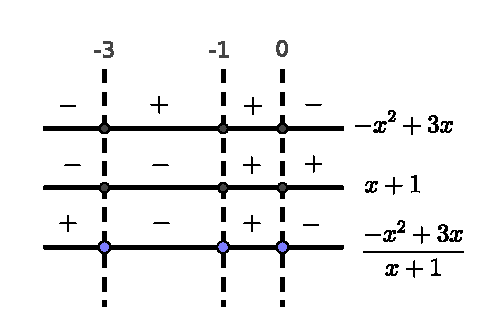
\includegraphics[width=8cm]{./cap_equacoes/figs/sinais}
 % \end{figure}

 Logo, pelo estudo de sinais acima, e considerando a restrição da inequação, obtemos o conjunto solução
\begin{equation*}
S= (-1, 0] \cup [3, +\infty).
\end{equation*}
 \end{exem}



\section{Sistema de inequações}

Algumas vezes, é necessário obter valores de $x$ que satisfazem duas ou mais inequações simultâneamente, o que denominamos \emph{sistema de inequações}. O conjunto solução de um sistema de inequações é a interseção dos conjuntos solução de cada inequação do sistema.

\begin{exem}
    $-1<2x-3\leqslant 3$

    Resolver esta inequação simultânea é equivalente à resolver o sistema:
    \begin{equation*}
    \left\{
        \begin{matrix}
            -1<2x-3\\
            2x-3\leqslant 3
        \end{matrix}
    \right.
    \end{equation*}

    A solução da primeira equação é $S_1=\{x\in\R \mid x>1\}=(1,+\infty)$ e da segunda equação é $S_2=\{x\in\R \mid x\leq 3\}=(-\infty,3]$. Fazendo a interseção das soluções:
    \begin{intervaloper}[3]{0}{4}
        \linelabel{1}{$S_1$}
        \linelabel{2}{$S_2$}
        \linelabel{3}{$S=S_1\cap S_2$}
        \dashes{1}{1}{3}
        \dashes{3}{1}{3}
        \interval{1}{10}{1}
        \interval{2}{02}{3}
        \intervalcolor{blue}
        \interval{3}{12}{1,3}
    \end{intervaloper}
    
    Logo, a solução geral do sistema é $S=S_1\cap S_2 = \{x\in\R \mid 1< x\leq 3\}=(1,3]$.
\end{exem}

\begin{exem}
    $3x+2<-x+3\leq x+4$

    Resolver esta inequação simultânea é equivalente à resolver o sistema:
    \begin{equation*}
    \left\{
        \begin{matrix}
            3x+2<-x+3\\
            -x+3\leq x+4
        \end{matrix}
    \right.
    \end{equation*}

    Assim, da 1ª equação temos
    \begin{equation*}
        3x+2<-x+3 \Rightarrow 4x<1 \Rightarrow x<\frac{1}{4}
    \end{equation*}
    e da 2ª equação
    \begin{equation*}
        -x+3\leq x+4 \Rightarrow -2x\leq 1 \Rightarrow x\geq -\frac{1}{2}.
    \end{equation*}

    Fazendo a interseção das soluções:
    \begin{intervaloper}[3]{-1}{1}
        \linelabel{1}{$S_1$}
        \linelabel{2}{$S_2$}
        \linelabel{3}{$S=S_1\cap S_2$}
        \dashes{-1/2}{1}{3}
        \dashes{1/4}{1}{3}
        \interval{1}{01}{1/4}
        \interval{2}{20}{-1/2}
        \intervalcolor{blue}
        \interval{3}{21}{-1/2,1/4}
    \end{intervaloper}
    
    Logo, a solução geral do sistema é $S=S_1\cap S_2 = \left[-\frac{1}{2}, \frac{1}{4} \right)$.
\end{exem}





 
%  \section{Inequações de 2º grau}
 
%  \begin{obs}
%   As inequações do 2º grau possuem uma das seguintes formas gerais
%  \begin{eqnarray*}
%  ax^2 + bx + c \leq 0 \\
%  ax^2 + bx + c < 0 \\
%  ax^2 + bx + c \geqslant 0 \\
%  ax^2 + bx + c >0 
%  \end{eqnarray*}  
%  para certos $a, b, c \in \R$ dados, com $a \neq 0$.
% \end{obs}
  
%  A principal diferença entre as equações de 2º grau e as inequações de 2º grau é que a equação, quando possui solução tem uma ou duas soluções, equanto que a inequação quando possui solução possui infinitas soluções, que representam um intervalo real ou a união de dois intervalos reais. 
 
%  Vejamos alguns exemplos de como resolver inequações do 2º grau, é importante ressaltar que para resolver inequações do 2º grau precisamos das técnicas de resoluções de equações do 2º grau, as quais foram apresentadas e exemplificadas anteriormente.
 
 
%  \begin{exem}
%  $x^2 + x - 20 \geqslant 0$
 
%  Resolvendo a equação $x^2 + x - 20 = 0$ obtemos que
% \begin{equation*}
% x^2 + x - 20  = (x+5) \cdot (x-4) . 
% \end{equation*}
 
%  Observemos que, $x+5> 0 \Leftrightarrow x> -5$ e que $x-4> 0 \Leftrightarrow x>4$. 
 
%  Portanto, temos três intervalos reais para analisar o sinal da inequação $x^2 + x - 20 \geqslant 0$, são eles $(-\infty, -5)$, $(-5, 4)$ e $(4, \infty)$. Para facilitar esta análise considere a seguinte tabela:

 
%  \begin{table}[H]
%  \centering
%  \begin{tabular}{|c|c|c|c|} \hline
%  \rowcolor{gray}
%                       & $(-\infty, -5)$ & $(-5, 4)$ & $(4, \infty,)$ \\ \hline
%                 $x+5$ & $-$             & $+$       & $+$ \\ \hline
%                 $x-4$ & $-$             & $-$       & $+$ \\ \hline
%  $(x+5) \cdot (x-4)$  & $+$             & $-$       & $+$ \\ \hline
%  \end{tabular}
%  \end{table}
 
%  Portanto, o conjunto solução desta inequação é o conjunto $(-\infty, -5] \cup [4, \infty)$, podemos também representar este conjunto solução por $S= \left\{ x \in \R \mid x \leqslant -5 \text{ ou } x \geqslant 4 \right\}$.
%  \end{exem}
 
 
 
%  \begin{exem}
%  $x^2 - 16 < 0$
 
%  \begin{eqnarray*}
%  x^2 - 16 < 0 \Leftrightarrow x^2 < 16 \Leftrightarrow \abs{x} < \sqrt{16} \Leftrightarrow -4 < x < 4
%  \end{eqnarray*}
 
% Portanto, o conjunto solução desta inequação é o conjunto $(-4, 4)$, podemos também representar este conjunto solução por $S= \left\{ x \in \R \mid -4 < x < 4 \right\}$. 
%  \end{exem}
 
%  \begin{exem}
%  $(x-2)^2 < 3x -2$
 
%  Simplificando a inequação obtemos:
%  \begin{eqnarray*}
%  (x-2)^2 < 3x -2 \Leftrightarrow x^2 -4x + 4 < 3x - 2 \Leftrightarrow x^2-4x-3x+4+2<0 \Leftrightarrow x^2-7x+6<0 \\
%  \end{eqnarray*}
%   Resolvendo a equação $x^2-7x+6= 0$ obtemos que
% \begin{equation*}
% x^2-7x+6 = (x-1) \cdot (x-6) . 
% \end{equation*}
 
%  Observemos que, $x-1> 0 \Leftrightarrow x>1$ e que $x-6> 0 \Leftrightarrow x >6$. 
 
%  Portanto, temos três intervalos reais para analisar o sinal da inequação $x^2-7x+6 < 0$, são eles $(-\infty, 1)$, $\left(1, 6 \right)$ e $\left(6, \infty\right)$. Para facilitar esta análise considere a seguinte tabela:
 
%  \begin{table}[H]
%  \centering
%  \begin{tabular}{|c|c|c|c|} \hline
%  \rowcolor{gray}
%     & $(-\infty, 1)$ & $\left(1, 6 \right)$ & $\left(6, \infty \right)$ \\ \hline
%                 $x-1$ & $-$             & $+$       & $+$ \\ \hline
%                 $x-6$ & $-$             & $-$       & $+$ \\ \hline
%   $(x-1) \cdot (x-6)$ & $+$             & $-$       & $+$ \\ \hline
%  \end{tabular}
%  \end{table}
 
%  Portanto, o conjunto solução desta inequação é o conjunto $(1 , 6)$, podemos também representar este conjunto solução por $S= \left\{ x \in \R \mid 1 < x < 6 \right\}$.
%  \end{exem}
 
%  \begin{exem}
%  $x^2-x+1>0$
 
%  Note que a equação $x^2-x+1= 0$ possui $\Delta= -3 < 0$ portanto esta equação não possui solução real. Neste caso para resolver a inequação $x^2-x+1>0$, podemos por exemplo utilizar o completamento de quadrados, com o qual obtemos que:

%  \begin{eqnarray*}
%  x^2-x+1>0 \Leftrightarrow \left(x - \dfrac{1}{2} \right)^2 + \dfrac{3}{4} > 0.
%  \end{eqnarray*}
%  Sabemos que $\left(x - \dfrac{1}{2} \right)^2 > 0$ para qualquer $x \in \R$, e que ao somar números positivos o resultado é um número positivo, com isso podemos concluir que $\left(x - \dfrac{1}{2} \right)^2 + \dfrac{3}{4} > 0$ para qualquer $x \in \R$. Portanto o conjunto solução da inequação $x^2-x+1>0$ é $S= \R= (-\infty, \infty)$.
 
%  Vale observar, aproveitando as contas acima, que a inequação $x^2-x+1<0$ não possui solução, logo para esta inequação temos $S= \emptyset$.
 
%  \end{exem}



%  \section{Inequações racionais}

% \begin{obs}
%   As inequações racionais são inequações dadas por quocientes/razões de polinômios. Como por exemplo:
%   \[\dfrac{p(x)}{q(x)} > 0\]
%   onde $p(x)$ e $q(x)$ são polinômios na variável $x$, com $q(x) \neq 0$. 
  
%   Aqui podemos trocar $>$ por $<$, $\leq$ ou $\geqslant$ e contínuamos com uma inequação.    
% \end{obs}
 
%  Lembramos que não existe divisão por $0$ (zero), logo estas inequações estão definidas apenas no conjunto
%   \[D= \{ x \in \R \mid  q(x) \neq 0\} \ . \]  
%   Este subconjunto $D$ dos números Reais no qual a inequação esta definida é chamado domínio da inequação. O conjunto solução da inequação é necessariamente um subconjunto do domínio da inequação.
  
%   Quando ambos os lados de uma inequação racional são não nulos, como por exemplo $\dfrac{p(x)}{q(x)} > 3$, um dos possíveis caminhos a se seguir na resolução da inequação é multiplicar ambos os lados da inequação por $q(x)$, mas para fazer isso corretamente é necessário levar em consideração o sinal de $q(x)$, o que nos força a quebrar a resolução em casos, daremos um exemplo de como fazer isso. Mas para evitar este tipo de problema temos como sugestão seguir os seguintes passos:
%   \begin{enumerate}[1)]
%   \item Mova todos os termos para o lado esquerdo da inequação, ficando com $0$ do lado direito;
%   \item Escreva a expressão resultante no lado esquerdo como uma única fração, com numerador e denominador fatorados;
%   \item Determine o domínio da inequação resultante;
%   \item Determine as raízes do numerador e denominador (quando for o caso) e use-os para definir os extremos dos intervalos;
%   \item Construa uma tabela, relacionando os sinais de cada fator em cada um dos intervalos, use esta tabela para fazer o estudo de sinal da inequação racional.
%   \item Determine a solução da inequação racional com base nas informações obtidas na tabela.
%   \end{enumerate}
 
% 	Após a realização dos dois primeiros passos listados acima, obtemos uma inequação de uma das seguintes formas:
% 	\begin{eqnarray}
% 	\dfrac{p(x)}{q(x)} \leq 0 \\
% 	\dfrac{p(x)}{q(x)} \geqslant 0
% 	\end{eqnarray}
% nas quais o lado direito é zero. Assim para chegar ao conjunto solução basta fazer a análise de sinal da expressão $\dfrac{p(x)}{q(x)}$, para isso consideramos os seguintes casos:

% Caso 1:	$\dfrac{p(x)}{q(x)} > 0$ se $p(x)$ e $q(x)$ tem o mesmo sinal, ou seja, nos seguintes conjuntos 
% \[ S_1= \{x \in \R \mid p(x)>0 \text{ e } q(x)>0 \} \]
% ou
% \[ S_2= \{x \in \R \mid p(x)<0 \text{ e } q(x)<0 \} \]
% logo o conjunto solução da inequação neste caso é $S= S_1 \cup S_2$.

% Caso 2:	$\dfrac{p(x)}{q(x)} < 0$ se $p(x)$ e $q(x)$ tem sinais opostos, ou seja, nos seguintes conjuntos 
% \[ R_1= \{x \in \R \mid p(x)>0 \text{ e } q(x)<0 \} \]
% ou
% \[ R_2= \{x \in \R \mid p(x)<0 \text{ e } q(x)>0 \} \]
% logo o conjunto solução da inequação neste caso é $S= R_1 \cup R_2$.
	
 
%  \begin{exem}
%   $4 - \dfrac{x^2+x+4}{x+1} \leq 0$
%   Antes de começar a resolver a inequação vamos determinar seu domínio. Neste caso para que a inequação esteja bem definida precisamos ter $x+1 \neq 0$ o que é satisfeito para $x \neq -1$. Portanto o domínio desta inequação é:
%   \[D= \{x \in \R \mid x \neq -1\} \ .\]
  
%   Para resolver a inequação começamos tirando o minímo múltiplo comum das duas frações para poder efetuar a soma das frações, lembrando que quando o denominador não aparece ele é um.

%   \[4 - \frac{x^2+x+4}{x+1} \leq 0 \Rightarrow
%     \frac{4x+4-x^2-x-4}{x+1} \leq 0 \Rightarrow
%     \frac{-x^2 + 3x}{x+1} \leq 0
%   \]
%   Agora vamos calcular os zeros de cada uma das equações $-x^2 + 3x$ e $x+1$ separadamente para poder fazer o estudo de sinal do quociente entre elas.
% \begin{equation*}
% x+1=0 \Leftrightarrow x= -1
% \end{equation*}
% \begin{equation*}
% -x^2 + 3x= 0 \Leftrightarrow x(-x+3)=0 \Leftrightarrow x=0 \ \ \text{ou} \ \ x=-3
% \end{equation*}

% Aqui alternativamente a tabela faremos o estudo de sinal da inequação quociente graficamente, que pode ser mais fácil para algumas pessoas visualizar o resultado.
% \begin{center}
%     \signtable[3]{-3,-1,0}{-1,1,1,-1}{-1,-1,1,1}{$-x^2+3x$}{$x+1$}{$\frac{-x^2+3x}{x+1}$}[2]
% \end{center}

%  %   \begin{figure}[H]
%  % \centering
%  % 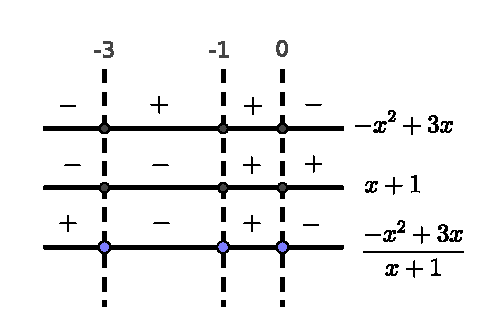
\includegraphics[width=8cm]{./cap_equacoes/figs/sinais}
%  % \end{figure}

%  Logo pelo jogo de sinais da figura acima, e considerando o domínio da inequação, obtemos
% \begin{equation*}
% S= [-3, -1) \cup [0, +\infty)
% \end{equation*}
%  como conjunto solução desta inequação.

%  \end{exem}

\begin{secExercicios}

\begin{exer}
   Resolva as inequações em $\R$:
    \begin{enumerate}[a)]
        \item $x + 1 \leq 7 - 3x < \dfrac{x}{2}-1$
        \item $3x+4 < 5 < 6-2x$
        \item $2-x<3x+2<4x+1$
        \item $(x-5)(3x-9)(-2x+8)<0$
        \item $-2x(x-1)(3x+4)<0$
        \item $\dfrac{x}{x-2}>3$
        \item $(2x-1)^3(x+2)>0$
        \item $(x-2)^2 \geq 0$
        \item $(x-\sqrt{2})(2x+3)(x-1)\geq0$
        \item $\dfrac{(2-5x)(x+1)}{(-x+3)}\leq 0$
        \item $\dfrac{x}{x+1} - \dfrac{x}{x-1} \geq 0$
        \item $\dfrac{2x}{x+2} > 2$
        \item $\dfrac{2}{x+1} + \dfrac{1}{x-1} \leq \dfrac{3}{x}$
    \end{enumerate}
\end{exer}

\begin{exer}
    Determine o os valores de $x$ no conjunto dos números naturais $\N$ que satisfazem
    \begin{equation*}
        5x-9<3x+1
    \end{equation*}
\end{exer}


\begin{exer}
    Determine o conjunto solução da inequação:
    \begin{equation*}
        \frac{x+1}{2}<5+x\leq \frac{2x-1}{4}.
    \end{equation*}
\end{exer}

\begin{exer}
    Resolva as inequações:
    \begin{enumerate}[a)]
        \item $(4x+5)^5<0$
        \item $(-3x-12)^4>0$
        \item $(x+6)^6\leq 0$
        \item $(x-2)^8(3-x)^5(4x+1)^7>0$
    \end{enumerate}
\end{exer}

\begin{exer}
    (Fuvest-SP) Resolva a inequação
    \begin{equation*}
        \frac{x^2-x-1}{\sqrt{x^2-3x}}\geq 0.
    \end{equation*}
\end{exer}

\begin{exer}
    Resolva os sistemas de inequações em $\R$:
    \begin{enumerate}[a)]
        \item  $\left\{
        \begin{matrix}
            3x-2 > 4x+1\\
            5x+1 \leq 2x-5
        \end{matrix}
    \right.$
        \item $\left\{
        \begin{matrix}
            5x-2 <0\\
            3x+1 \geq 4x-5\\
            x-3 \geq 0
        \end{matrix}
    \right.
    $
        \item $\left\{
        \begin{matrix}
            3x+2 \geq 5x - 2\\
            4x-1 > 3x-4\\
            3-2x < x-6
        \end{matrix}
    \right.$
        \item  $\left\{
        \begin{matrix}
            \dfrac{2x-5}{1-x} \leq -2\\
            \dfrac{x^2 + x + 3}{x+1} > x
        \end{matrix}
    \right.$
    \end{enumerate}
\end{exer}
\end{secExercicios}

%\subsection*{Respostas:}
%\shipoutAnswer
%\setcounter{chapter}{6} 
 \chapter{Módulo}

 \section{Expressões algébricas modulares}

 Dois números reais podem ser associados por um número real chamado de ``distância''. Podemos observar (de modo intuitivo) que a distância dos pontos $-x$ e $x$ até a origem (zero) é a mesma e, matematicamente, chamada de \textbf{valor absoluto}\index{Valor absoluto|see{Módulo}}\index{Módulo}, ou \textbf{módulo}, do número $x$, e é representada por $\abs{x}$. Assim, dizemos que:
\begin{itemize}
\item O valor absoluto de $-3$ é $3$, ou seja, $\abs{-3}= 3$ (a distância do -3 até a origem é 3);
\item O valor absoluto de $3$ é $3$, ou seja, $\abs{3}= 3$ (a distância do 3 até a origem é 3);
\end{itemize}
\begin{obs}
Generalizando esta ideia definimos que:
\begin{equation}
\label{eq:modulo}
\abs{x}= \left\{\begin{array}{rl}
      -x , & \text{se} \ \ x<0 \\
      x , & \text{se} \ \ x \geq 0
     \end{array}\right. .
     \end{equation}
\end{obs}

Em termos práticos, quando analisamos $|x|$ pelo lado direito da Equação \ref{eq:modulo}, dizemos que ``abrimos o módulo''.

Se precisamos trabalhar com o valor absoluto ou módulo de um número real, levamos em conta as seguintes propriedades:

\begin{prop}[Propriedades do módulo]
 Para quaisquer $x, y \in \R$, são válidas as seguintes propriedades: \label{prop.modulo}
\begin{enumerate} \begin{multicols}{2}
 \item $\abs{x} \geq 0$;
 \item $\abs{x}= 0 \Leftrightarrow x= 0$;
 \item $x \leq \abs{x}$;
 \item $-x \leq \abs{x}$;
 \item $\abs{-x}= \abs{x}$;
 \item $\abs{x}^2= x^2$;
 %, de fato,\\
 %se $x \geq 0$, pela definição do módulo temos que $\abs{x}= x$ e daí $\abs{x}^2= x^2$, \\
 %se $x < 0$, pela definição do módulo temos que $\abs{x}= -x$ e daí $\abs{x}^2=(-x)^2= x^2$.\\
 %Portanto, para todo $x \in \R$, $\abs{x}^2= x^2$.

 \item $\abs{x^n}= \abs{x}^n$, se $n$ é par;%, de fato, \\
 %se $x \geq 0$, pela definição do módulo temos que $\abs{x}= x$ e daí $\abs{x}^n= x^n$, \\
 %se $x < 0$, pela definição do módulo temos que $\abs{x}= -x$ e daí $\abs{x}^n= (-x)^n= x^n$.\\
 %Portanto, para todo $x \in \R$, $\abs{x}^n= x^n$.

 \item $\abs{x \cdot y}= \abs{x} \cdot \abs{y}$;%, de fato,
%\begin{equation*}
%\abs{x \cdot y}^2= (x \cdot y)^2= x^2 \cdot y^2= \abs{x}^2 \cdot \abs{y}^2= (\abs{x} \cdot \abs{y})^2 \ .
%\end{equation*}
 %Como $\abs{x \cdot y} \geqslant 0$ e $\abs{x} \cdot \abs{y} \geqslant 0$ resulta
%\begin{equation*}
%\abs{x \cdot y}= \abs{x} \cdot \abs{y} \ . 
%\end{equation*}

 \item $\abs{\dfrac{x}{y}}= \dfrac{\abs{x}}{\abs{y}}$, para $y \neq 0$;%, de fato,
%\begin{equation*}
%\abs{\dfrac{x}{y}}^2= \left(\dfrac{x}{y} \right)^2= \dfrac{x^2}{y^2}= \dfrac{\abs{x}^2}{\abs{y}^2}= \left( \dfrac{\abs{x}}{\abs{y}} \right)^2 \ . 
%\end{equation*}
% Como $\abs{\dfrac{x}{y}} \geq 0$ e $\dfrac{\abs{x}}{\abs{y}} \geq 0$ resulta que
%\begin{equation*}
%\abs{\dfrac{x}{y}}= \dfrac{\abs{x}}{\abs{y}} \ .
%\end{equation*}

 \item \emph{Desigualdade triangular}:\\ $\abs{x+y}\leq \abs{x}+\abs{y}$; %, de fato, \\
 %se $x + y \geqslant 0$, pela definição de módulo, $\abs{x+y}= x+y \leq \abs{x} + \abs{y}$; \\
 %se $x + y < 0$, pela definição de módulo, $\abs{x+y}= -(x+y)= -x-y \leq \abs{x} + \abs{y}$. \\
 %Logo, para quaisquer $x, y \in \R$ temos que
%\begin{equation*}
%\abs{x+y} \leq \abs{x}+\abs{y} \ .
%\end{equation*}

 \item $\abs{x-y} \leq \abs{x} + \abs{y}$;%, de fato \\
 %Note que $x-y= x+ (-y)$, logo $\abs{x-y}= \abs{x+ (-y)}$ aplicando a desigualdade trinagular temos,
%\begin{equation*}
%\abs{x-y}= \abs{x+ (-y)} \leq \abs{x} + \abs{-y}= \abs{x} + \abs{y} \ .
%\end{equation*}

 \item $\abs{\abs{x} - \abs{y}} \leq \abs{x - y}$%, para mostrar esta desigualdade vamos fazer por partes.
 %\begin{itemize}
 %\item $\abs{x} - \abs{y} \leq \abs{x - y}$, \\
 %de fato, pela desigualdade triangular temos que
%\begin{equation*}
%\abs{z+y} \leq \abs{z} + \abs{y}
%\end{equation*}
% subtraíndo $\abs{y}$ a ambos os termos temos,
%\begin{equation*}
%\abs{z+y} - \abs{y} \leq \abs{z}
%\end{equation*}
% fazendo $x= z+y$ temos que $z=x-y$ substituindo estes valores na equação acima obtemos
%\begin{equation*}
%\abs{x} - \abs{y} \leq \abs{x-y} \ . 
%\end{equation*}
 \item $\abs{y} - \abs{x} \leq \abs{x - y}$.%, \\
 %de fato, pela desigualdade triangular temos que
%\begin{equation*}
%\abs{x+z} \leq \abs{x} + \abs{z}
%\end{equation*}
% subtraíndo $\abs{x}$ a ambos os termos temos,
%\begin{equation*}
%\abs{x+z} - \abs{x} \leq \abs{z}
%\end{equation*}
 %fazendo $y= x+z$ temos que $z=y-x$ substituindo estes valores na equação acima obtemos
%\begin{equation*}
%\abs{y} - \abs{x} \leq \abs{y-x}= \abs{x-y} \ . 
%\end{equation*}
%\end{itemize}

% Portanto,
%\begin{equation*}
% \abs{\abs{x} - \abs{y}} = \pm (\abs{x} - \abs{y}) \leq \abs{x-y} \ .
%\end{equation*}
\end{multicols}
\end{enumerate}
\end{prop}

 Você pode se deparar, em alguns momentos, com expressões matemáticas que envolvem módulo. Elas são chamadas de expressões matemáticas modulares. É preciso entender que operar com módulo pode ser algo bastante complicado e, para fugir disso, o que se faz, na prática, é ``abrir o módulo'' usando a definição dada pela Equação \ref{eq:modulo}. Vejamos os exemplos a seguir.

 \begin{exem}
  Reescreva a expressão $\dfrac{\abs{x}}{x}$ eliminando o módulo.

  Primeiramente, observe que devemos considerar $x \neq 0$, pois a expressão apresenta uma divisão por $x$ (e não podemos dividir por 0). Relembrando a definição de $|x|$ dada na Equação \ref{eq:modulo}, concluímos que os casos a serem analisados são: $x<0$ e $x>0$.

  \begin{itemize}
   \item Caso $x> 0$. Para este caso temos $\abs{x}= x$ e a expressão pode ser reescrita como
\begin{equation*}
\dfrac{\abs{x}}{x}=\dfrac{x}{x}= 1.
\end{equation*}
   \item Caso $x< 0$. Para este caso, temos $\abs{x}= -x$ e a expressão pode ser reescrita como
\begin{equation*}
\dfrac{\abs{x}}{x}=\dfrac{-x}{x}= -1.
\end{equation*}
  \end{itemize}

 Portanto, podemos reescrever a expressão $\dfrac{\abs{x}}{x}$ da seguinte maneira:

 \begin{equation*}
   \frac{\abs{x}}{x} = \left\{ \begin{array}{rl}
        -1, & \text{se} \ \ x< 0 \\
         1, & \text{se } \ \ x> 0
     \end{array}\right..
 \end{equation*}
\end{exem}
 
 \begin{exem}
Reescreva a expressão modular $\abs{-5x^5}$ eliminando o módulo.

Usando as propriedades e a definição de módulo podemos escrever
\begin{equation*}
\abs{-5x^5}= \abs{-5}\cdot \abs{x^5}= 5 \cdot \abs{x^5} = \left\{ \begin{array}{rl}
        5 x^5, & \text{se} \ \ x^5\geq 0 \\
         5 (-x^5), & \text{se } \ \ x^5< 0
     \end{array}\right.
     = \left\{ \begin{array}{rl}
        5 x^5, & \text{se} \ \ x\geq 0 \\
         -5x^5, & \text{se } \ \ x< 0
     \end{array}\right..
\end{equation*}
 Observe que, como o expoente é ímpar, devemos considerar a possibilidade de $x^5$ ser um número positivo ou negativo (e isso está diretamente ligado ao fato de $x$ ser positivo ou negativo).
 \end{exem}
 
 \begin{exem}
  $\abs{-5x^4}$
\begin{equation*}
\abs{-5x^4}= \abs{-5}\cdot \abs{x^4}= \abs{-5}\cdot \abs{x}^4 = 5 \cdot x^4.
\end{equation*}

Observe que foram usadas as propriedades 5 ($\abs{-5} = 5$) e 7 ($\abs{x^4} = \abs{x}^4$). E como o expoente é par, o valor de $x^4$ é positivo, independente do sinal de $x$. Neste caso, $\abs{x^4} = x^4$. 
 \end{exem}
 
 \begin{exem}
  Simplifique a expressão $\abs{\dfrac{2x^2y}{4xy^3}}$ usando propriedades de módulo:
\begin{equation*}
\abs{\dfrac{2x^2y}{4xy^3}} = \abs{\dfrac{x}{2y^2}}= \dfrac{\abs{x}}{\abs{2y^2}}= \dfrac{\abs{x}}{\abs{2} \cdot \abs{y^2}}= \frac{\abs{x}}{2 \cdot y^2}.
\end{equation*}
 \end{exem}
 
 \begin{exem}
 Simplifique a expressão  $\dfrac{\abs{-6x}}{5} - \abs{\dfrac{-3x}{2}}$ usando propriedades de módulo:

 \begin{eqnarray*}
  \dfrac{\abs{-6x}}{5} - \abs{\dfrac{-3x}{2}} &=&
 \dfrac{\abs{-6}\cdot \abs{x}}{5} - \dfrac{\abs{-3} \cdot \abs{x}}{\abs{2}} \\
 &=& \dfrac{6 \cdot \abs{x}}{5} - \dfrac{ 3 \cdot \abs{x}}{2} \\
 &=& \dfrac{12 \cdot \abs{x}}{10} - \dfrac{15 \cdot \abs{x}}{10} \\
 &=& \dfrac{12\abs{x} - 15\abs{x}}{10} \\
 &=& \dfrac{-3\abs{x}}{10}.
 \end{eqnarray*}

\end{exem}

 \begin{exem}
  Simplifique a expressão $\abs{x-2} + \abs{x+4}$ \label{eqmodulo}

 Para simplificar esta expressão, primeiro precisamos usar a definição de módulo para cada um dos termos que estão sendo somados:
 \begin{align*}
    \abs{x-2} = \left\{\begin{array}{rl}
      -(x-2), & \text{se} \ \ x-2< 0 \\
      x-2, & \text{se } \ \ x-2 \geq 0
     \end{array} \right.
     &\Rightarrow
     \abs{x-2} =  \left\{\begin{array}{rl}
      -x + 2, & \text{se} \ \ x < 2 \\
      x-2, & \text{se } \ \ x \geq 2
     \end{array}\right.\\
      \abs{x+4} =  \left\{\begin{array}{rl}
      -(x+4), &\text{se} \ \ x+4< 0 \\
      x+4, & \text{se } \ \ x+4 \geq 0
     \end{array}\right.
     &\Rightarrow
     \abs{x+4} =  \left\{\begin{array}{rl}
      -x - 4, & \text{se} \ \ x < -4 \\
      x + 4, & \text{se } \ \ x \geq -4
     \end{array}\right.
  \end{align*}

  Observe que $(x-2)$ muda de sinal quando $x=2$, e que $(x+4)$ muda de sinal quando $x=-4$, logo esta soma de módulos tem uma definição particular para cada um dos intervalos $(-\infty, -4)$, $[-4, 2)$ e $[2, \infty)$. Para facilitar a compreensão organizamos na tabela seguinte a soma, em cada caso.

   \begin{table}[H]
 \centering
 \begin{tabular}{|c|c|c|c|} \hline
 \rowcolor{gray}
  Expressão & $(-\infty, -4)$ & $[-4, 2)$ & $[2, \infty)$  \\\hline
  $\abs{x-2}$ & $-x+2$ &  $-x+2$ & $x-2$ \\\hline
  $\abs{x+4}$ & $-x-4$ &  $x+4$ & $x+4$ \\\hline
  $\abs{x-2} + \abs{x+4}$ & $-x+2-x-4$ & $-x+2+x+4$ & $x-2+x+4$ \\\hline
 \end{tabular}
\end{table}

 Portanto, temos que
 \begin{equation*}
 \abs{x-2} + \abs{x+4} =  \left\{ \begin{array}{rl}
      -2x-2, & \text{se} \ \ x < -4 \\
      6, &\text{se } \ \ -4 \leq x < 2 \\
      2x + 2, & \text{se} \ \ x \geq 2 
     \end{array}\right..
 \end{equation*} 
 \end{exem}


 \section{Equações modulares}

\begin{obs}
  As equações modulares são equações que apresentam expressões dentro de um módulo. Em particular, vamos analisar casos em que esta expressão matemática é um polinômio. Por exemplo, temos
  \[\abs{p(x)}= 0.\]

  Assim como nas equações de 1º e 2º grau vistas no Capítulo 5, resolver uma equação modular significa encontrar todos os valores de $x$ que tornam a equação verdadeira (satisfazem a equação), considerando um conjunto universo específico (por exemplo, os reais).
 \end{obs}

 Antes de começarmos a ver exemplos destas equações lembremos que para um número real $x$ qualquer:

 \[
\abs{x}= \left\{\begin{array}{rl}
      -x , & \text{se} \ \ x<0 \\
      x , & \text{se} \ \ x \geq 0
     \end{array}\right. .
\]

Além disso, lembre-se que todas as propriedades listadas em \ref{prop.modulo} são válidas e podem ser usadas durante a resolução de uma equação modular.

Os exemplos a seguir resolvem equações modulares para um melhor entendimento.

\begin{exem} 
  Suponha que $a> 0$. Resolva a equação $\abs{x}= a$.

Vamos analisar a equação considerando os casos $x\geq 0$ e $x < 0$.

Para $x\geq 0$, temos $\abs{x} = x = a$.

Para $x<0$, temos $\abs{x} = -x = a$, ou seja, $x = -a$.

Portanto o conjunto solução desta equação é $S= \left\{-a, a \right\}$.
\end{exem}

\begin{exem}
  Resolva $\abs{x}= 10$ (observe que este é um caso particular do exemplo anterior).

 Novamente, vamos analisar a equação considerando os casos $x\geq 0$ e $x < 0$.

Para $x\geq 0$, temos $\abs{x} = x = 10$.

Para $x<0$, temos $\abs{x} = -x = 10$, ou seja, $x = -10$.

Portanto o conjunto solução desta equação é $S= \left\{-10, 10 \right\}$.
\end{exem}

\begin{exem}
 Resolva a equação $\abs{2x-2}= 10$.

Vamos analisar a equação considerando os casos $2x - 2 \geq 0$ e $2x - 2 < 0$, ou seja, $x \geq 1$ e $x < 1$.

Para $x\geq 1$ temos $\abs{2x-2} = 2x-2$. Assim, $$\abs{2x-2} = 10 \Leftrightarrow 2x - 2 = 10 \Leftrightarrow 2x = 12 \Leftrightarrow x = 6.$$

Para $x < 1$ temos $\abs{2x-2} = -(2x-2)= -2x+2$. Assim, $$\abs{2x-2} = 10 \Leftrightarrow -2x + 2 = 10 \Leftrightarrow -2x = 8 \Leftrightarrow x = -4.$$

Portanto, o conjunto solução desta equação é $S= \left\{-4, 6 \right\}$.
 \end{exem}
 
 \begin{exem}
 Resolva $\abs{2x^2 - 72}= 26$.

Observe que, aplicando a definição de módulo, podemos reescrever o lado esquerdo da equação como:

\begin{equation}
\label{ex:mod_quadratico}
\abs{2x^2 - 72} = \left\{\begin{array}{rl}
2x^2 - 72, & \mbox{se} \; \;  2x^2 - 72 \geq 0\\
-(2x^2 - 72), & \mbox{se} \; \; 2x^2 - 72 < 0
\end{array}\right. \end{equation}

Desse modo, devemos fazer um estudo de sinal e decidir os intervalos em que $2x^2 - 72$ é positivo, negativo ou nulo (se ainda tem dúvida em como fazer isso, consulte o Capítulo 6). Para este estudo, reescrevemos $2x^2 - 72$ em sua forma fatorada, ou seja, $$2x^2 - 72 = 2(x+6)(x-6) = (2x+ 12)(x-6)$$.

\begin{signtbl}{3}{2}
        \linelabel{1}{$2x+12$}
        %\numbernode{6}{1}{2}
        \numbernode{-6}{1}{1}
        \numbernode{6}{3}{2}
        \signs{1}{-1,1,1}
        \linelabel{2}{$x-6$}
        %\numbernode{-6}{2}{1}
        \numbernode{6}{2}{2}
        \numbernode{-6}{3}{1}
        \signs{2}{-1,-1,+1}
        \intervalcolor{violet}
        \signs{3}{1,-1,+1}
        \linelabel{3}{$(2x+12)(x-6)$}
        \intervalsign{3}{02}{1}
        \intervalsign{3}{20}{2}
\end{signtbl}

Resumindo, a análise de sinal nos permite avaliar que:

     \[
     \begin{cases}
      2x^2- 72 \geq 0, \ \ \text{se} \ \ x \leq -6 \; \; \mbox{ou} \; \; x \geq 6\\
      2x^2- 72 < 0, \ \ \text{se} \ \ -6 < x < 6
      \end{cases}
     \]
Podemos então reescrever a Expressão \ref{ex:mod_quadratico} como:

\begin{equation}
\abs{2x^2 - 72} = \left\{\begin{array}{rl}
2x^2 - 72, & \mbox{se} \; \;  2x^2 - 72 \geq 0\\
-(2x^2 - 72), & \mbox{se} \; \; 2x^2 - 72 < 0
\end{array}\right. = \left\{\begin{array}{rl}
2x^2 - 72, & \mbox{se} \; \;  x \leq -6 \; \; \mbox{ou} \; \; x \geq 6\\
-2x^2 + 72, & \mbox{se} \; \; -6 < x < 6
\end{array}\right. \end{equation}

Temos, portanto, duas equações para resolver separadamente.

Se $x\leq 6$ ou $x \geq 6$ então
\begin{equation*}
2x^2- 72= 26 \Leftrightarrow 2x^2= 98 \Leftrightarrow x^2= 49 \Leftrightarrow x= - 7\; \mbox{ou} \; \; x = 7.
\end{equation*}

     Note que as duas soluções pertencem ao intervalo que estamos considerando a análise ($x = 7$ está no intervalo $x \geq 6$ e $x = -7$ está no intervalo $x\leq -6$) e, portanto, elas são de fato soluções da equação.

Se $-6 < x < 6$ então
      \begin{eqnarray*}
      -(2x^2-72)= 26 \Leftrightarrow -2x^2 + 72= 26 \Leftrightarrow -2x^2= -46 \\
     \Leftrightarrow x^2= 23 \Leftrightarrow x= -\sqrt{23} \; \; \mbox{ou} \; \;  x = \sqrt{23}.
      \end{eqnarray*}

Note que $\sqrt{23} \approx 4,78$ e que, portanto, temos $-6 < -\sqrt{23} < \sqrt{23} < 6$, ou seja, ambas as soluções encontradas pertencem ao intervalo de análise e podem ser consideradas. Juntando as análises intervalares realizadas podemos concluir que o conjunto solução da equação modular $\abs{2x^2 - 72|}$ é 
\begin{equation*}
S= \{-7, -\sqrt{23}, \sqrt{23}, 7\}.
\end{equation*}
\end{exem}

\begin{exem}
 \colorbox{yellow}{Atenção! O cojunto solução de uma equação modular pode ser vazio.} Resolva $\abs{x-4}=-2$.

Perceba que, pela Propriedade 1 podemos afirmar que o módulo de qualquer número é sempre maior ou igual a zero. Desse modo, não há valor de $x$ que torne $\abs{x-4} = -2$. Só com essa análise podemos concluir que o conjunto solução é $S = \{  \}$. Ou podemos apenas dizer que não há solução para esta equação.

Alguém mais curioso poderia se questionar se não há como encontrar o conjunto vazio como solução de maneira algébrica. Se este for o caso, faríamos a seguinte resolução:

Pela definição de módulo temos que
     \[
    \abs{x-4} = \left\{\begin{array}{rl}
    -(x-4), & \text{se} \ \ x-4 < 0 \\
    x-4, & \text{se } \ \ x-4 \geq 0
     \end{array}\right.
     =
    \left\{\begin{array}{rl}
    -x+4, & \text{se} \ \ x < 4 \\
    x-4, & \text{se } \ \ x \geq 4
     \end{array}\right..
     \]
     Então, 
     \[
     \abs{x-4} = -2 \Leftrightarrow \left\{\begin{array}{rl}
    -x+4=-2, & \text{se} \ \ x < 4 \\
    x-4 = -2, & \text{se } \ \ x \geq 4
     \end{array}\right.
     \Leftrightarrow \left\{\begin{array}{rl}
     x = 6, & \text{se} \ \ x < 4 \\
    x = 2, & \text{se } \ \ x \geq 4
     \end{array}\right.
     \]
 Observe que, na condição $x<4$ encontramos $x = 6$, ou seja, não há solução neste intervalo. De modo análgo, encontramos a solução $x = 2$ para o intervalo $x \geq 4$, o que não faz sentido. Concluímos, portanto, que a equação não tem solução (ou que o conjunto solução é vazio).
\end{exem}

 Vamos agora colocar, de forma mais geral, o que acabamos de ver nos exemplos. A vantagem de entender este processo de forma geral é que você poderá usá-lo na resolução de qualquer equação modular. 
 
 Consideremos uma equação modular na forma geral
\begin{equation*}
\abs{A}= B,
\end{equation*}
 em que $A$ e $B$ são expressões algébricas quaisquer. Pela definição de módulo temos que
 \[ \abs{A}= \begin{cases}
          -A, \ \text{se} \ \ A < 0 \\
           A, \ \text{se} \ \ A \geq 0
         \end{cases}.
 \]
 Logo, as soluções da equação modular devem satisfazer
\begin{equation*}
A= B \ \ \ \text{ou} \ \ \ -A= B \ .
\end{equation*}
 Além disso, lembremos que, por propriedade de módulo, $\abs{A}\geq 0$, independente da expressão $A$.
 
 Como nossa equação é da forma  $\abs{A}= B$, logo garantir $\abs{A}\geq 0$ é equivalente a garantir $B \geq 0$, donde obtemos que as equações com $B < 0$ não possuem solução.

 Resumindo, temos que uma variável $x$ é solução da equação modular $\abs{A}= B$ se ela satisfizer:
\begin{equation*}
(A= B \ \ \ \text{ou} \ \ \ -A= B) \ \ \ \text{e} \ \ \ (B \geq 0) \ . 
\end{equation*}

 Vejamos mais um exemplo resolvido de equação modular.

 \begin{exem}
   Resolva $\abs{x-2} + \abs{x+4}= 10$.

   Observe que temos $A = \abs{x-2} + \abs{x+4}$ e $B = 10$. Como $B > 0$, basta analisar os casos $A= B$ e $-A= B$.

   $A$ é composto pela soma de duas expressões modulares vistas no Exemplo \ref{eqmodulo}. Ao abrirmos o módulo, obtivemos a expressão 
   \[ \abs{x-2} + \abs{x+4} = \left\{\begin{array}{rl}
      -2x-2, & \text{se} \ \ x < -4 \\
      6, & \text{se } \ \ -4 \leq x < 2 \\
      2x + 2, & \text{se} \ \ x \geq 2 \ .
     \end{array}\right..
  \]
 Para resolver a equação modular  dada faremos a análise para cada intervalo.

 \textbf{Intervalo 1:} $x < -4$

 Neste caso, $\abs{x-2} + \abs{x+4}= -2x-2$, ou seja, 
\begin{equation*}
-2x-2= 10 \Leftrightarrow -2x= 12 \Leftrightarrow x= -6.
\end{equation*}
 Como $x= -6$ pertence ao intervalo $x< -4$, ela é uma solução a ser considerada.

 \textbf{Intervalo 2:} $-4 \leq x < 2$

 Neste caso, $\abs{x-2} + \abs{x+4}= 6$, e nossa equação se torna $6= 10$. Isto é impossível, donde concluímos que neste intervalo a equação não tem solução (parece estranho? Isto significa que não há nenhum número real entre -4 e 2 que torna a expressão $\abs{x-2} + \abs{x+4}$ igual a 6).

 \textbf{Intervalo 3:} $x \geq 2 $

 Neste caso, $\abs{x-2} + \abs{x+4}= 2x + 2$ e, então,
\begin{equation*}
2x + 2= 10 \Rightarrow 2x= 8 \Rightarrow x= 4.
\end{equation*}

Como $x= 4$ pertence ao intervalo $x \geq 2$, ela será uma solução a ser considerada.

 Portanto, após a análise das soluções nos três intervalos concluímos $S=\{-6, 4\}$ como  o conjunto solução da equação modular
$\abs{x-2} + \abs{x+4}= 10.$
 \end{exem}


 \section{Inequações modulares}

 Nesta seção usaremos as propriedades da ordem do conjunto dos números reais e também as propriedades de módulo de um número real. Neste momento já supomos que o leitor está bem familiarizado com as tais propriedades.%, mas na dúvida você pode consultar as propriedades que estão listadas nas %\ref{prop.ordem} e \ref{prop.modulo}.

Vejamos a seguir alguns exemplos de inequações modulares.

 \begin{exem} 
  Suponha que $a> 0$. Resolva a inequação $\abs{x} < a$.

Faremos esta resolução de modo semelhante ao que fizemos para a resolução das equações modulares, levando em conta, agora, o sinal da desigualdade.

Mais uma vez, lembre-se que 
 \[
\abs{x}= \left\{\begin{array}{rl}
      -x , & \text{se} \ \ x<0 \\
      x , & \text{se} \ \ x \geq 0
     \end{array}\right. .
\]

Para resolver a inequação, vamos analisar os dois intervalos que aparece ao abrirmos o módulo.

\textbf{Intervalo 1:} $x < 0$

Neste caso temos a desigualdade $-x < a$ e, portanto, $x > -a$. Como estamos procurando soluções na região onde $x$ é estritamente negativo, nos limitaremos aos valores que satisfaçam as duas condições: $x < 0$ e $x > -a$. Ou seja, neste intervalo temos como solução o conjunto $S_1 = \{x \in \R | \ -a < x < 0\}$.

\textbf{Intervalo 2:} $x\geq 0$

Neste caso temos a desigualdade $x<a$, que já se resolve de forma direta. Perceba que, como nossa região de análise são os números estritamente positivos, a solução deve considerar ambas as desigualdades ($x \geq 0$ e $x < a$). Ou seja, neste intervalo temos como solução o conjunto $S_2 = \{x \in \R | \ 0 \leq x < a\}$.

Assim, o conjunto solução da inequação dada é o conjunto constituído pelas soluções encontradas no Intervalo 1 unido com as soluções encontradas no Intervalo 2. Faremos então uma união de conjuntos e, portanto, $S = S_1 \cup S_2 = \{x \in \R| -a < x < a\} = (-a,a)$.

\begin{comment}
\begin{equation*}
\abs{x} < a \Leftrightarrow \abs{x}^2 < a^2 \Leftrightarrow x^2 < a^2
\end{equation*}
   mas,
\begin{equation*}
x^2 < a^2 \Leftrightarrow x^2 - a^2 < 0 \Leftrightarrow (x-a)(x+a) < 0 \ .
\end{equation*}
   Vamos então analisar quando $(x-a)(x+a) < 0$. Lembremos que produto de dois números é negativo quando um deles for negativo e o outro positivo, com isso a inequação $(x-a)(x+a) < 0$ é satisfeita em duas situações:\\
   Caso 1: $x-a<0$ e $x+a>0$
\begin{equation*}
x-a<0 \Rightarrow x< a
\end{equation*}
   e
\begin{equation*}
x+a>0 \Rightarrow x>-a \Rightarrow -a< x
\end{equation*}
  Fazendo a interseção dos conjuntos $A_1= \left\{ x \in \R \mid x<a \right\}$ e $B_1= \left\{ x \in \R \mid -a<x \right\}$, obtemos $A_1 \cap B_1= \left\{ x \in \R \mid -a< x <a \right\}$. O conjunto $A_1 \cap B_1$ é o conjunto solução da inequação neste caso.


   Caso 2: $x-a>0$ e $x+a<0$
\begin{equation*}
x-a> 0 \Rightarrow x> a
\end{equation*}
   e
\begin{equation*}
x+a< 0 \Rightarrow x<-a
\end{equation*}
   Fazendo a interseção dos conjuntos $A_2= \left\{ x \in \R \mid x> a \right\}$ e $B_2= \left\{ x \in \R \mid x<-a \right\}$, obtemos $A_2 \cap B_2= \emptyset$. Portanto neste caso a inequação não possui solução.

  Portanto $\abs{x} < a \Leftrightarrow -a< x <a$.
\end{comment}
  \end{exem}
  
\begin{exem}
   Caso particular: Resolva $\abs{x} \leq 5$.
\begin{equation*}
\abs{x} \leq 5 \Leftrightarrow -5 \leq x \leq 5.
\end{equation*}
  Logo, o conjunto solução desta inequação é
\begin{equation*}
S=\{x \in \R| -5 \leq x \leq 5\} = [-5, 5]. 
\end{equation*}
\end{exem}

\begin{exem}
   Suponha que $a> 0$. Resolva a inequação $\abs{x} > a$.

Faremos esta resolução de modo semelhante ao que fizemos para a resolução das equações modulares, levando em conta, agora, o sinal da desigualdade.

Mais uma vez, lembre-se que 
 \[
\abs{x}= \left\{\begin{array}{rl}
      -x , & \text{se} \ \ x<0 \\
      x , & \text{se} \ \ x \geq 0
     \end{array}\right. .
\]

Para resolver a inequação, vamos analisar os dois intervalos que aparece ao abrirmos o módulo.

\textbf{Intervalo 1:} $x < 0$

Neste caso temos a desigualdade $-x > a$ e, portanto, $x < -a$. Como estamos procurando soluções na região onde $x$ é estritamente negativo, nos limitaremos aos valores que satisfaçam as duas condições: $x < 0$ e $x < -a$. Ou seja, neste intervalo temos como solução o conjunto $S_1 = \{x \in \R | x < -a\} = (-\infty, -a)$.

\textbf{Intervalo 2:} $x\geq 0$

Neste caso temos a desigualdade $x>a$, que já se resolve de forma direta. Perceba que, como nossa região de análise são os números estritamente positivos, a solução deve considerar ambas as desigualdades ($x \geq 0$ e $x > a$). Ou seja, neste intervalo temos como solução o conjunto $S_2 = \{x \in \R | x > a\} = (a, +\infty)$.

Assim, o conjunto solução da inequação dada é o conjunto constituído pelas soluções encontradas no Intervalo 1 unido com as soluções encontradas no Intervalo 2. Faremos então uma união de conjuntos e, portanto, $S = S_1 \cup S_2 = \{x \in \R| x < -a \ \ \mbox{ou} \ \ x > a\} = (-\infty,a) \cup (a, + \infty)$.

\begin{comment}
\begin{equation*}
\abs{x} > a \Leftrightarrow \abs{x}^2 > a^2 \Leftrightarrow x^2 > a^2
\end{equation*}
   mas,
\begin{equation*}
x^2 > a^2 \Leftrightarrow x^2 - a^2 > 0 \Leftrightarrow (x-a)(x+a) > 0 \ .
\end{equation*}
   Vamos então analisar quando $(x-a)(x+a) > 0$. Lembremos que produto de dois números é positivo quando eles tem o mesmo sinal, com isso a inequação $(x-a)(x+a) > 0$ é satisfeita em duas situações:\\
   Caso 1: $x-a< 0$ e $x+a< 0$
\begin{equation*}
x-a< 0 \Rightarrow x< a
\end{equation*}
   e
\begin{equation*}
x+a< 0 \Rightarrow x< -a \ .
\end{equation*}
  Fazendo a interseção dos conjuntos $A_1= \left\{ x \in \R \mid x<a \right\}$ e $B_1= \left\{ x \in \R \mid x< -a \right\}$, obtemos $A_1 \cap B_1= \left\{ x \in \R \mid x< -a \right\}$. O conjunto $A_1 \cap B_1$ é o conjunto solução da inequação neste caso.


   Caso 2: $x-a> 0$ e $x+a> 0$
\begin{equation*}
x-a> 0 \Rightarrow x> a
\end{equation*}
   e
\begin{equation*}
x+a> 0 \Rightarrow x> -a 
\end{equation*}
   Fazendo a interseção dos conjuntos $A_2= \left\{ x \in \R \mid x> a \right\}$ e $B_2= \left\{ x \in \R \mid x> -a \right\}$, obtemos $A_2 \cap B_2= \left\{ x \in \R \mid x> a \right\}$. O conjunto $A_2 \cap B_2$ é o conjunto solução da inequação neste caso.

   Agora fazendo $S= (A_1 \cap B_1) \cup (A_2 \cap B_2)$ obtemos que $S= \left\{ x \in \R \mid x<-a \text{ ou } x> a \right\}$ é o conjunto solução da inequação $\abs{x} > a$.

  Portanto $\abs{x} > a \Leftrightarrow x<-a \text{ ou } x> a$.
\end{comment}
\end{exem}

\begin{exem}
   Caso particular: Resolva $\abs{x} \geq 5$.

Pelo caso estudado anteriormente podemos afirmar que \begin{equation*}
\abs{x} \geq 5 \Leftrightarrow x \leq -5 \ \ \text{ ou } \ \ x \geq 5.
\end{equation*}
   
Logo, o conjunto solução desta inequação é:
\begin{equation*}
S= \{x \in \R| x \leq -5 \ \ \mbox{ou} \ \ x > 5\}= (-\infty, -5] \cup [5, \infty) \ . 
\end{equation*}
 \end{exem}
 
%  \section{Equações radicais ou irracionais}
%  \colorbox{blue}{
%  \begin{minipage}{0.9\linewidth}
%  \begin{center}
%   As equações radicais são equações nas quais temos polinômios dentro de raízes. Como por exemplo:
%   \[\sqrt[n]{p(x)}= 0\]
%   onde $n \in \N$ e $p(x)$ é um polinômio na variável $x$. Caso $n \in \N$ seja par precisamos ainda ter $p(x) \geqslant 0$.
%  \end{center}
%  \end{minipage}}
% 
%%  Lembre-se que não existe raíz de ordem par de número negativo, logo a equação radical
%  \[\sqrt[n]{p(x)}= 0\]
%  caso $n \in \N$ seja par, está definida apenas no conjunto $D= \{x \in \R \mid p(x) \geqslant 0\}$.
% 
%%  Este subconjunto dos números reais no qual a equação está bem definida é chamado de domínio da equação. A solução de uma equação radical é necessariamente um subconjunto do domínio da mesma.
% 
%%  \begin{exem}
%  $\dfrac{1}{\sqrt{x}}= 4$
% 
%%  Para resolver esta equação começamos determinando seu domínio. Note que aqui precisamos ter duas condições sendo satisfeitas:
%  \begin{enumerate}[i)]
%  \item $\sqrt{x} \neq 0 \Rightarrow x \neq 0$;
%  \item $x \geqslant 0$ pois temos uma raíz de ordem $2$.
%  \end{enumerate}
%  O domínio será portanto a interseção dos dois conjuntos acima que é dado por:
%  \[D= \{ x \in \R \mid x > 0 \} \ . \]
% 
%%  Vamos agora resolver a equação, 
%  \[\dfrac{1}{\sqrt{x}}= 4 \Rightarrow \left(\dfrac{1}{\sqrt{x}}\right)^2= 4^2 \Rightarrow \dfrac{1}{x}= 16 \Rightarrow \dfrac{1}{16}= x\]
% 
%%  Como $\dfrac{1}{16} \in D$ esta é de fato a solução da equação.
%  \end{exem}
% 
%  \section{Inequações radicais ou irracionais}
% 
%   \vskip0.3cm
%  \colorbox{blue}{
%  \begin{minipage}{0.9\linewidth}
%  \begin{center}
%   As inequações radicais são inequações nas quais temos polinômios dentro de raízes. Estas inequações possuem domínios com as mesmas restrições das equações radicais.
%  \end{center}
%  \end{minipage}}
%  \vskip0.3cm
 
\begin{secExercicios}

 \begin{exer}
    Simplifique as expressões, eliminando o módulo:
    \begin{enumerate}[a)] \begin{multicols}{2}
        \item $\dfrac{|x-1|}{x-1}$
        \item $\dfrac{|x+3|}{x+3}$
        \item $\dfrac{|x|}{x}+\dfrac{|x-4|}{x-4}$
        \item $\dfrac{\abs{x-3}}{x-3}$
        \item $1 + \dfrac{\abs{x-2}}{x-2}$
        \item $\dfrac{\abs{x}}{x}, \; 0 < x < 4$
       \end{multicols} \end{enumerate}
\end{exer}

 \begin{exer}
    Resolva as desigualdades, em cada caso:
    \begin{enumerate}[a)]
        \item $\abs{x} < 1$
        \item $\abs{1-5x} <4$
        \item $\abs{7x-4} <10$
        \columnbreak
        \item $\abs{x-2} < -2.\abs{-x}$
        \item $\abs{3+9x} <1$
        \item $\abs{3x+4}\leq 2$
        \item $\abs{4x-4} \geq 2$
        \item $\abs{x+5} >2$
        \item $\abs{2-4x} \geq 3$
        \item $\abs{x-3} > -1$
    \end{enumerate}
\end{exer}


\begin{exer}
    Resolva a equação dada:
    \begin{enumerate}[a)]
        \item $\abs{x} = 1248$
        \item $\abs{x} = -2$
        \item $\abs{x-5} = 4$
        \item $\abs{x}= 2.\abs{-x}$
        \item $\abs{2x-4} = 6$
        \item $\abs{3x+1}=\abs{x-2}$
        \item $\abs{6-3x} = 10$
        \item $\abs{(x-1)(x+2)} = 0$
    \end{enumerate}
\end{exer}


\begin{exer}
    Determine o conjunto solução das seguintes equações:
    \begin{enumerate}[a)]
        \item $\abs{\dfrac{x-2}{3}} =5$
        \item $\abs{\dfrac{1-x}{4}}=6$
        \item $\abs{2x-3} = \abs{4x+5}$
        \item $\abs{5x-4} = \abs{3x+6}$
        \item $\abs{2x+5} = \abs{x-11}$
        \item $\abs{x-3} + \abs{x+4} = 7$
        \item $\abs{x-3} + \abs{x-4}=1$
        \item $\abs{\abs{x-5} -8} = 6$
    \end{enumerate}
\end{exer}





\begin{exer}
    As afirmações abaixo são verdadeiras ou falsas? Justifique sua resposta.
    \begin{enumerate}[a)]
        \item $\abs{a}$ é sempre um número positivo.
        \item $\abs{a}$ pode ser um número negativo.
        \item $\abs{a} = a$, para todo número $a$ real.
        \item $\abs{x}$ pode ser zero.
        \item $\abs{a.b.c} = \abs{a}.\abs{b}.\abs{c}$
        \item $\abs{a.b} < \abs{a}\abs{b}$, para quaisquer $a,b$ reais.
        \item $\abs{a + b} = \abs{a} + \abs{b}$, para quaisquer $a, b$ reais.
        \item $\abs{-2 + c} = 2 + \abs{c}$, para todo $c \leq 0$.
     \end{enumerate}
\end{exer}

\end{secExercicios}

%\subsection*{Respostas:}

%\shipoutAnswer

%%Este trabalho está licenciado sob a Licença Creative Commons Atribuição-CompartilhaIgual 4.0 Internacional. Para ver uma cópia desta licença, visite https://creativecommons.org/licenses/by-sa/4.0/ ou envie uma carta para Creative Commons, PO Box 1866, Mountain View, CA 94042, USA.

\markboth{\sffamily\normalsize\bfseries Respostas dos Exercícios}{\sffamily\normalsize\bfseries Respostas dos Exercícios} % Set the page headers to display a Bibliography chapter name
\addcontentsline{toc}{chapter}{\textcolor{ocre}{Respostas dos Exercícios}}
\chapter*{Respostas dos Exercícios}
%\addcontentsline{toc}{Part}{Respostas dos Exercícios}
%\fancyhead[RE]{Introdução à Matemática Superior}
%\fancyhead[LO]{RESPOSTAS DOS EXERCÍCIOS}
%\fancyhead[LE,RO]{\thepage}

Devido a construção deste material, muitas respostas ainda não foram incluídas, podem conter imprecisões e erros.

\setlength{\columnseprule}{1pt}

\begin{multicols}{2}
\shipoutAnswer
\end{multicols}

\setlength{\columnseprule}{0pt}



% \setcounter{part}{2}
\part{Polinômios}
%\setcounter{chapter}{7} 
 \chapter{Polinômios}

\begin{obs}
  Um polinômio $p$ na incógnita $x$ e com coeficientes reais $\R$ é uma expressão da forma
\begin{equation*}
p(x)= a_nx^n + a_{n-1}x^{n-1}+ \ldots + a_1x+ a_0= \sum_{i=0}^{n} a_ix^i ,
\end{equation*}
  em que os coeficientes $a_n, \ldots, a_0 \in \R$, $a_n \neq 0$ e $n \in \N$. O número natural $n$ é chamado de grau do polinômio $p$, e escreve-se $gr(p)= n$. O termo $a_0$ é denominado termo constante de $p$.
\end{obs}

  Caso necessário, podemos tomar polinômios com coeficientes no conjunto dos números complexos $\C$.

 Os termos polinômio e função polinomial serão considerados como sinônimos e utilizados sem distinção no decorrer deste texto.

 Uma função polinomial de grau $0$ é uma função constante; uma função polinomial de grau $1$ é uma função linear (ou, função afim); uma função polinomial de grau $2$ é uma função quadrática.

 %Por simplicidade, a partir de agora iremos considerar nossos polinômios sobre $\R$, porém esta teoria pode ser estendida sem muita dificuldade para o corpo dos números complexos.

 \begin{obs}
 Dados um número real $k$ e o polinômio $p(x)= a_nx^n + a_{n-1}x^{n-1}+ \ldots + a_1x+ a_0$, chama-se \emph{valor numérico de $p$ em $k$} ao valor:
\begin{equation*}
p(k)= a_nk^n + a_{n-1}k^{n-1}+ \ldots + a_1k+ a_0 \ .
\end{equation*}
 \end{obs}

\begin{exem}
Se considerarmos o polinômio $p(x)= x^2 + 7x+10$, ele tem grau $2$ e temos os seguintes valores numéricos para $p$:
\begin{eqnarray*}
p(-6)&=& (-6)^2 + 7(-6) +10= 4\\
p(-5)&=& (-5)^2 + 7(-5) +10= 0\\
p(-4)&=& (-4)^2 + 7(-4) +10= -2\\
p(-2)&=& (-2)^2 + 7(-2) +10= 0\\
p(0)&=& 0^2 + 7 \cdot 0 +10= 10\\
\end{eqnarray*}
\end{exem}

 \begin{obs}
 Em particular, se $k$ é um número real tal que $p(k)= 0$, dizemos que $k$ é uma \emph{raiz} ou \emph{um zero} de $p$.
 \end{obs}

 \begin{exem}
 No caso $p(x)= x^2 + 7x+10$, temos que $k_1= -5$ e $k_2=-2$ são raízes do polinômio $p(x)= x^2 + 7x+10$.
 \end{exem}

  \begin{obs}
  O polinômio nulo (ou identicamente nulo) é um polinômio da forma cujos coeficientes são todos nulos, ou simplesmente, $p(x)= 0$. Por convenção, o grau deste polinômio será indefinido.
 \end{obs}


\begin{teo}
  Sejam $p$ e $q$ dois polinômios em $\R$, dados por:
\begin{align*}
p(x)&= a_nx^n + a_{n-1}x^{n-1}+ \ldots + a_1x+ a_0= \sum_{i=0}^{n} a_ix^i,\\
q(x)&= b_nx^n + b_{n-1}x^{n-1}+ \ldots + b_1x+ b_0= \sum_{i=0}^{n} b_ix^i.
\end{align*}
  
  Temos que $p=q$ se, e somente se, cada um dos coeficientes coincidem, isto é, $a_i= b_i$ para todo $i \in \{0, 1, 2, \cdots, n\}$.
 \end{teo}
 \begin{proof}
 Para todo $x \in \R$, temos:
\begin{gather*}
a_i= b_i \Leftrightarrow a_i - b_i=0 \Leftrightarrow (a_i - b_i)x^i=0 \Leftrightarrow \sum_{i=0}^{n}(a_i - b_i)x^i= 0 \Leftrightarrow\\
 \sum_{i=0}^{n}a_i x^i - \sum_{i=0}^{n}b_i x^i = 0 \Leftrightarrow \sum_{i=0}^{n}a_i x^i = \sum_{i=0}^{n}b_i x^i \Leftrightarrow p(x)= q(x).\qedhere
\end{gather*}
 \end{proof}

  Este teorema mostra que, quando escrevemos um polinômio $p$ na forma
\begin{equation*}
p(x)= a_nx^n + a_{n-1}x^{n-1}+ \ldots + a_1x+ a_0
\end{equation*}
 com $a_i \in \R$, então os números $a_0, \ldots, a_n$ são determinados de modo único.

\section{Operações com polinômios}

\subsection{Adição e subtração}
 Sejam $p$ e $q$ dois polinômios
\begin{align*}
p(x)&= a_nx^n + a_{n-1}x^{n-1}+ \ldots + a_1x+ a_0= \sum_{i=0}^{n} a_ix^i,\\
q(x)&= b_nx^n + b_{n-1}x^{n-1}+ \ldots + b_1x+ b_0= \sum_{i=0}^{n} b_ix^i
\end{align*}

A adição e subtração de polinômios é feita a partir da adição e subtração dos coeficientes correspondentes a um mesmo grau, ou seja,
\begin{align*}
(p+q)(x)&= (a_n+ b_n)x^n + (a_{n-1}+b_{n-1})x^{n-1}+ \ldots + (a_1+b_1)x+ (a_0+b_0)= \sum_{i=0}^{n} (a_i+b_i)x^i\\
(p-q)(x)&= (a_n- b_n)x^n + (a_{n-1}-b_{n-1})x^{n-1}+ \ldots + (a_1-b_1)x+ (a_0-b_0)= \sum_{i=0}^{n} (a_i-b_i)x^i.
\end{align*}

\begin{exem}
    Sejam $p(x)=2x^3-x^2+2$ e $q(x)=2x^5-7x^3+x-1$. Assim,
    \begin{align*}
        (p+q)(x)=2x^5-5x^3-x^2+x+1\\
        (p-q)(x)=-2x^5+9x^3-x^2-x+3.
    \end{align*}
\end{exem}

  \begin{prop}
  Se $p$, $q$ e $p+q$ são polinômios não nulos, então o grau do polinômio $p+q$ é menor ou igual ao maior dos números $gr(p)$ e $gr(q)$. Ou seja,
\begin{equation*}
gr(p+q) \leq \text{max}\{gr(p), gr(q)\} \ .
\end{equation*}
  \end{prop}

\subsection{Multiplicação}
A multiplicação entre polinômios é feita pela propriedade distributiva da multiplicação em relação à adição e multiplicação.

\begin{exem}
    Sejam $p(x)=2x-1$ e $q(x)=5x^2+2x-2$. Então,
    \begin{equation*}
        p(x)\cdot q(x)= (2x-1)(5x^2+2x-2) = 10x^3+4x^2-4x-5x^2-2x+2=10x^3-x^2-6x+2.
    \end{equation*}
\end{exem}

  \begin{prop}
  Se $p$, $q$ e $p \cdot q$ são polinômios não nulos, então o grau do polinômio $p \cdot q$ é igual a soma dos graus de $p$ e $q$;
\begin{equation*}
gr(p \cdot q) = gr(p) + gr(q) \ .
\end{equation*}
  \end{prop}

\subsection{Divisão}

Lembre que dividir um número inteiro $D$ (dividendo) por outro inteiro $d$ (divisor) diferente de zero consiste em encontrar dois números inteiros $q$ (quociente) e $r$ (resto), com $0\leqslant r<d$, tais que:
$D=qd+r$

Por exemplo, $7$ dividido por $2$ é $7=3\cdot 2 +1$, com quociente $3$ e resto $1$.

Da mesma forma, a divisão de um polinômio $p(x)$ por outro $d(x)$, com $d(x)\neq 0$, consiste em encontrar um par de polinômios $q(x)$ e $r(x)$ tais que satisfazem a equação
\begin{equation*}
    p(x)=q(x) d(x) +r(x)
\end{equation*}
em que $gr(r)<gr(d)$ ou $r(x)=0$. É garantido que sempre existe um único par de polinômios $q(x)$ e $r(x)$ com estas condições.

Chamamos de $p(x)$ o dividendo, $d(x)$ o  divisor, $q(x)$ o quociente e $r(x)$ o resto da divisão.

\begin{obs}
    A divisão é dita exata se $r(x)=0$. Neste caso, $p$ é divisível por $d$ ou $d$ é divisor de $p$.
\end{obs}

\begin{exem}
    A divisão do polinômio $p(x)$ por $x^2-3x$ resulta no quociente $x+2$ e resto $5$. Para descobrir $p(x)$ escrevemos
    \begin{equation*}
        p(x)=(x+2)(x^2-3x)+5 = x^3-3x^2+2x^2-6x+5=x^3-x^2-6x+5.
    \end{equation*}
\end{exem}

\begin{exem}
    Determine $m \ (m\neq 1)$ de modo que o polinômio $A(x)=(m-1)x^3-mx+2m+1$ seja divisível por $B(x)=x+1$.

    Veja que para ser divisível, o resto da divisão deve ser zero, isto é, $r(x)=0$. Como $m\neq 1$ então o dividendo tem grau 3, o divisor grau 1 e, portanto, o quociente tem grau 2. Denote por $q(x)=ax^2+bx+c$. Assim,
    \begin{equation*}
        (m-1)x^3-mx+2m+1 = (ax^2+bx+c)(x+1) = ax^3+(a+b)x^2+(b+c)x+c.
    \end{equation*}

    Igualando os coeficientes,
    \begin{equation*}
        \left\{
        \begin{matrix}
            a=m-1\\
            a+b=0\\
            b+c=-m\\
            c=2m+1
        \end{matrix}
        \right.
    \end{equation*}

    Assim, $b=-a=-m+1$ e $b=-m-c=-m-(2m+1)=-3m-1$. Portanto,
    \begin{gather*}
        -m+1=-3m-1\\
        3m-m=-1-1\\
        2m=-2\\
        m=-1.
    \end{gather*}
\end{exem}

\textbf{Método da chave:} Efetuar o a divisão pelo método da chave consiste em seguir os seguintes passos:
\begin{enumerate}
    \item Escreva os polinômios (dividendo e divisor) em ordem decrescente dos seus expoentes e completá-los, quando necessário, com termos de coeficiente zero.
    \item Dividir o termo de maior graus do dividendo pelo de maior grau do divisor, o resultado será um termo do quociente.
    \item Multiplicar o termo obtido no passo 2 pelo divisor e subtrair esse produto do dividendo;
    \item Se o grau da diferença for menor do que o do divisor, a diferença será o resto da divisão e o processo termina;
    \item Senão, retorne ao passo 2, considerando a diferença como um novo dividendo.
\end{enumerate}

\begin{exem}
    Encontre o quociente de $p(x)=2x^3 +3x-1$ por $d(x)=x^2+2x+5$.
    \begin{center}
    \polylongdiv[style=D]{2x^3 +3x-1}{x^2+2x+5}
    \end{center}
\end{exem}

\begin{exem}
    Encontre o quociente de $p(x)=x^3-4x^2+x+6$ por $d(x)=x+1$.
    \begin{center}
    \polylongdiv[style=D]{x^3-4x^2+x+6}{x+1}
    \end{center}
\end{exem}


\textbf{Dispositivo de Briott-Ruffini:} Este método é utilizado para calcular a divisão de um polinômio $p(x)$ por um polinômio de 1º grau da forma $x-a$. Como o grau do resto é sempre menor que o do divisor, então o resto deve ser um número $r\in\R$.

Este método será ilustrado pelo exemplo a seguir.

\begin{exem}
    Considere a divisão de $p(x)=3x^3-5x^2+x-2$ por $x-2$. Este método trabalha apenas com os coeficientes do polinômio $p(x)$ e com a raiz do divisor $x-2$, ou seja, o número $2$.

    \begin{enumerate}
        \item Colocamos a raiz do divisor seguida dos coeficientes do dividendo em ordem decrescente das potências de $x$. Repetimos o primeiro coeficiente do dividendo na linha de baixo.
        \begin{center}
            \polyhornerscheme[x=2,tutor=true,stage=2,tutorstyle=\color{red},showbase=top]{3x^3-5x^2+x-2}
        \end{center}

        \item  Multiplicamos a raiz do divisor pelo coeficiente repetido e adicionamos o produto com o segundo coeficiente, colocando o resultado abaixo dele.
        \begin{center}
            \polyhornerscheme[x=2,tutor=true,stage=4,tutorstyle=\color{red}, tutorlimit=2,showbase=top]{3x^3-5x^2+x-2}
        \end{center}

        \item Repetimos o processo anterior com os 3º e 4º coeficientes do dividendo, sucessivamente.
        \begin{center}
            \polyhornerscheme[x=2,tutor=true,stage=6,tutorstyle=\color{red}, tutorlimit=2,showbase=top]{3x^3-5x^2+x-2}
            \hspace{2cm}
            \polyhornerscheme[x=2,tutor=true,stage=8,tutorstyle=\color{red}, tutorlimit=2,showbase=top]{3x^3-5x^2+x-2}
        \end{center}

        \item O último número obtido é o resto da divisão e os outros números à esquerda são os coeficientes do quociente.
        \begin{center}
            \polyhornerscheme[x=2,resultbottomrule,resultleftrule,resultrightrule,showbase=top,showmiddlerow=false]{3x^3-5x^2+x-2}
        \end{center}
    \end{enumerate}
    
    Logo, $q(x)=3x^2+x+3$ e o resto é $r=4$.
\end{exem}

\begin{exem}
    Vamos determine o resto da divisão de $x^6-1$ por $x+1$. Pelo dispositivo de Briott-Rufini
    \begin{center}
            \polyhornerscheme[x=-1,resultbottomrule,resultleftrule,resultrightrule,showbase=top,showmiddlerow=false,equalcolwidths=true]{x^6-1}
        \end{center}

    Assim, o resto da divisão é zero.
\end{exem}

\section{Teorema do Resto}

\begin{teo}[Teorema do Resto]
    O resto da divisão de um polinômio $p(x)$ por um binômio $x-a$ é igual ao valor numérico de $p(x)$ em $x=a$, isto é, $p(a)=r$.
\end{teo}
\begin{proof}
    Como o grau do resto é sempre menor que o do divisor, então o resto deve ser um número $r\in\R$. Assim, $p(x)=(x-a)q(x)+r$ e
    \begin{equation*}
        p(a)=(a-a)q(a)+r=0\cdot q(a)+r=r.\qedhere
    \end{equation*}
\end{proof}

\begin{teo}[Teorema de D'Alembert]
    Um polinômio $p(x)$ é divisível por $x-a$ se, e somente se, $p(a)=0$.
\end{teo}

\begin{exem}
    O polinômio $p(x)=x^3+4x^2+x-6$ é divisível por $x+2$ pois $p(-2)=(-2)^3+4(-2)^2-2-2=0$.
\end{exem}

% \todo[inline]{PAREI AQUI}
% ------------------

%   Para funções polinomiais o \emph{Teorema Fundamental da Álgebra} garante a existência de zeros.

%   \begin{teo}[Teorema Fundamental da Álgebra]
%   Seja $p \in \C[x]$ um polinômio não constante. Então existe um número complexo $z_0$ tal que $p(z_0)=0$.
%   \end{teo}

%   \begin{proof}
%   A demonstração deste resultado pode ser encontrada em livros de Cálculo de uma variável complexa ou Análise Complexa como por exemplo página 119 do (SOARES, 2009).
%   \end{proof}

%   Como consequência direta do Teorema Fundamental da Álgebra temos o seguinte teorema.

%   \begin{teo}
%   Todo polinômio de grau $n \geq 1$ possui pelo menos uma raiz real ou complexa.
%   \end{teo}

%  Observe que estes resultados garantem que todo polinômio possui pelo menos uma raiz complexa, como vamos focar nossos estudos em polinômios sobre $\R$, podemos neste caso ter polinômios que não possuem raízes reais. Ainda sobre as raízes de um polinômio vale destacar o seguinte teorema.

%  \begin{teo}
%   Seja $p$ um polinômio não nulo em $K$, escrito na forma
% \begin{equation*}
% p(x)= a_nx^n + a_{n-1}x^{n-1}+ \ldots + a_1x+ a_0
% \end{equation*}
%    então $p$ tem no máximo $n$ raízes em $K$.
%  \end{teo}

%  \begin{teo}
%   Sejam $p(x)$, $g(x)$ polinômios sobre o corpo $K$, i.e., polinômios em $K[x]$, e suponhamos que $gr(g) \geq 0$. Então, existem polinômios $q(x)$ e $r(x)$ tais que
% \begin{equation*}
% p(x)= q(x)g(x) + r(x) \ , 
% \end{equation*}
%   em que $gr(r) < gr (g)$. Essas condições permitem determinar os polinômio $q$ e $r$ de modo único.
%  \end{teo}

%  \begin{proof}
%  A demonstração deste teorema pode ser encontrada na página 58 do (LANG, 1972).
%  \end{proof}



%  \begin{exem}
%   Como um exemplo para a divisão de polinômios, façamos a divisão do polinômio $p_1(x)=x^3-4x^2+x+6$ pelo binômio $g_1(x)=x+1$:

%  \begin{figure}[H]
%  \centering
%  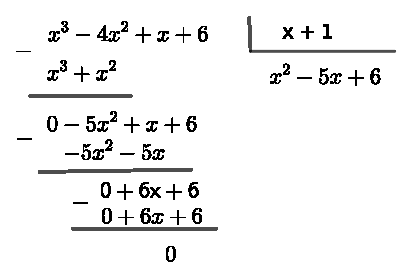
\includegraphics[width=8cm]{./cap_expralg/figs/polinomiosdivisao}
%  \end{figure}

%  note que o quociente da divisão é $q_1(x)= x^2 - 5x + 6$, e o resto desta divisão é $r(x)=0$ (zero). Como o resto é zero concluímos que $p_1(x)$ é divisível por $g_1(x)$. Portanto $p_1(x)= q_1(x)g_1(x)$, ou seja, $x^3-4x^2+x+6= (x^2-5x+6)(x+1)$.
%  \end{exem}

%  Como consequência do teorema anterior, temos o seguinte corolário, que nos garante que no exemplo anterior $-1$ é uma raiz do polinômio $p_1(x)$.

%  \begin{coro}
%  Seja $p$ um polinômio não-nulo sobre $K$. Seja $\alpha \in K$ tal que $p(\alpha)=0$. Então, existe um polinômio $q(x)$ sobre $K$ tal que
% \begin{equation*}
% p(x)= (x - \alpha)q(x) \ .
% \end{equation*}
%  \end{coro}

%  Como consequência deste Corolário, todo polinômio de grau $n \geq 1$ pode ser escrito como produto de $n$ fatores de grau $1$.

%  \begin{teo}[Teorema da Decomposição]
%   Todo polinômio $p(x)= a_nx^n + a_{n-1}x^{n-1}+ \ldots + a_1x+ a_0$, com $a_n \neq 0$, pode ser escrito de forma fatorada
% \begin{equation*}
% p(x)= a_n(x - r_1)(x - r_2) \ldots (x - r_n)
% \end{equation*}
%   onde $r_1, r_2, \cdots, r_n$ são as raízes do polinômio.
%  \end{teo}

\section{Equações polinomiais}

Dado um polinômio $p(x)$ de grau $n>0$, uma equação polinomial (ou algébrica) é uma equação da forma $p(x)=0$, ou seja, uma equação algébrica de grau $n$ é uma equações do tipo:
\begin{equation*}
    a_n x^n+a_{n-1} x^{n-1}+\cdots+ a_1 x+a_0=0.
\end{equation*}

O número $r$ é uma raiz da equação $p(x)=0$ se, e somente se, $p(r)=0$.

\begin{obs}
As equações algébricas de 1º e 2º grau já foram descritas. As equações de 3º grau possuem raízes descritas pelas fórmulas de Cardano; já as raízes das equações de 4º grau possuem raízes são obtidas pelas fórmulas de Ferrari.

As equações de grau superior a 4 não apresentam fórmulas resolutivas em termos dos coeficientes do polinômio.
\end{obs}

Ainda é possível que haja soluções para estas equações de grau 5 ou superior. Para funções polinomiais o \emph{Teorema Fundamental da Álgebra} garante a existência de zeros.

\begin{teo}[Teorema Fundamental da Álgebra]
Toda equação algébrica de grau $n$ admite um total de $n$ raízes complexas.
\end{teo}

Note que o teorema garante a existência de soluções complexas, mas não diz como obtê-las. Além disso, uma equação algébrica pode não possuir soluções reais.

\subsection{Multiplicidade de uma raiz e fatoração}

Dizemos que a equação $p(x)=0$ possui raiz $r$ de multiplicidade $m$, com $m\geqslant 1$, se, e somente se, podemos escrever
\begin{equation*}
    p(x)=(x-r)^m q(x) =0
\end{equation*}
tal que $q(r)\neq 0$. Ou seja, $p(x)$ é divisível por $(x-r)^m$.

\begin{exem}
    A equação $x^5\cdot (x+7)^3 = 0$ possui raízes $x=0$ com multiplicidade $5$ e $x=-7$ com multiplicidade 3.
\end{exem}

\begin{obs}
    Dado uma equação $p(x)=a_n x^n+a_{n-1} x^{n-1}+\cdots+ a_1 x+a_0=0$ de grau $n>0$ tal que $r_1,\dots,r_n$ são todas as raízes da equação (eventualmente com repetição quando a multiplicidade é maior que 1). Então, o polinômio $p(x)$ pode ser fatorado da forma:
    \begin{equation*}
        p(x)=a_n\cdot (x-r_1)\cdot (x-r_2) \cdots (x-r_n).
    \end{equation*}
\end{obs}

 \section{Equações racionais}

 \begin{obs}
  As equações racionais são dadas por quocientes/razões de polinômios da forma:
  \[\dfrac{p(x)}{q(x)}= 0\]
  onde $p(x)$ e $q(x)$ são polinômios na variável $x$ e $q(x) \neq 0$.
 \end{obs}
 
 Lembre-se que não podemos dividir por $0$ (zero), logo a equação racional
 \[\dfrac{p(x)}{q(x)}= 0\]
 está definida apenas no conjunto $D= \{x \in \R \mid q(x) \neq 0\}$.
 
 Este subconjunto dos números reais no qual a equação está bem definida é chamado de domínio da equação. A solução de uma equação racional é necessariamente um subconjunto do domínio da mesma.
 
 Vejamos alguns exemplos de como resolver uma equação racional.
 
 \begin{exem} $\dfrac{1}{x}= \dfrac{4}{3x} + 1$
 
 Para resolver esta equação começamos determinando seu domínio. Para isso lembremos que não existe divisão por $0$ (zero), logo um número real $x$ pertence ao domínio desta equação se, e somente se, 
 $x \neq 0$ e $3x \neq 0 \Rightarrow x \neq 0$.
 
 Portanto, o domínio desta equação é o conjunto
 \[D= \{ x \in \R \mid x \neq 0 \} \ . \]
 
 Agora vamos resolver a equação,
 \begin{eqnarray*}
 \dfrac{1}{x} = \dfrac{4}{3x} + 1.
 \end{eqnarray*}
 
 Precisamos tirar o MMC dos denominadores, pois os mesmos são diferentes
 \begin{eqnarray*}
 \dfrac{3}{3x}= \dfrac{4 + 3x}{3x} \\
 \dfrac{3-4-3x}{3x} = 0.
 \end{eqnarray*}
 
 Lembre que esta equação é zero somente quando o numerador for zero, logo basta olhar o numerador,
 \begin{eqnarray*}
 -1 = 3x \Rightarrow x= \dfrac{-1}{3}.
 \end{eqnarray*}
 
 Como $\frac{-1}{3} \in D$ decorre que o conjunto solução desta equação é $S= \left\{ \dfrac{-1}{3} \right\}$.
 \end{exem}
 
 % \begin{exem} $\dfrac{2x^2 - 6x}{x - x^3}= 0$
 
 % Calculando o domínio:
 % \begin{gather*}
 % x - x^3 \neq 0\\
 % x - x^3 = 0 \Leftrightarrow x(1-x^2)= 0 \Leftrightarrow x= 0 \text{ ou } x^2= 1 \Rightarrow x= \pm 1
 % \end{gather*}
 
 % Portanto, o domínio desta equação é o conjunto
 % \[D= \{ x \in \R \mid x \neq 0; x \neq 1; x \neq -1 \}= \R \setminus \{-1, 0, 1\}. \]
 
 % Agora vamos resolver a equação,
 % \begin{eqnarray*}
 % \dfrac{2x^2 - 6x}{x - x^3}= 0 \\
 % \dfrac{x(2x - 6)}{x(1 - x^2)}= 0 \\
 % \dfrac{2x - 6}{1 - x^2}= 0 \\
 % 2x - 6= 0 \\
 % x= 3.
 % \end{eqnarray*}
 
 % Como $3 \in D$ decorre que o conjunto solução desta equação é $S= \{ 3 \}$.
 % \end{exem}
 
 \begin{exem} $1 - \dfrac{2}{x}= \dfrac{8}{x^2}$
 
 Calculando o domínio. Um número real $x$ pertence ao domínio desta equação se:
 \begin{eqnarray*}
  x \neq 0 \text{ e } x^2 \neq 0 \Rightarrow x \neq 0
 \end{eqnarray*}
 
 Portanto, o domínio neste caso é
 \[D= \{ x \in \R \mid x \neq 0 \}= \R \setminus \{0\} \ . \]
 
 Agora vamos resolver a equação,
 \begin{eqnarray*}
 1 - \dfrac{2}{x}= \dfrac{8}{x^2} \\
 \dfrac{x^2}{x^2} - \dfrac{2x}{x^2}= \dfrac{8}{x^2} \\
 x^2 - 2x= 8 \\
 x^2 -2x -8= 0 \\
 (x-4)(x+2)= 0 \\
 x_1= 4 \text{ ou } x_2= -2.
 \end{eqnarray*}
 
 Como $\{-2, 4\} \subset D$ decorre que o conjunto solução desta equação é $S= \{ -2, 4 \}$.
 \end{exem}
 
 % \begin{exem} $\dfrac{x^3 -39x + 70}{x^2 + 2x - 8}= 0$
 
 % Calculando o domínio. 
 
 % Um número real $x$ pertence ao domínio desta equação se:
 % \begin{eqnarray}
 %  x^2 + 2x - 8 \neq 0 
 % \end{eqnarray}
 % como as raízes desta equação do 2º grau são $-4$ e $2$, decorre que o domínio neste caso é
 % \[D= \{ x \in \R \mid x \neq -4; x \neq 2 \}= \R \setminus \{-4, 2\} \ . \]
 
 % Vamos resolver a equação.
 
 % 1ª Forma: Note que a equação é satifeita quando o numerador for zero, logo basta resolver
 % \begin{eqnarray}
 % x^3 -39x + 70= 0 \\
 % (x+7)(x-2)(x-5)= 0 \\
 % x= -7 \text{ ou } x= 2 \text{ ou } x= 5
 % \end{eqnarray}
 
 % Agora precisamos verificar quais soluções da equação $x^3 -39x + 70= 0$ estão no conjunto $D$, note que $2 \notin D$ e $\{-7, 5\} \subset D$ portanto nosso conjunto solução é:
 % \[S= \{ -7, 5 \} \ . \]
 
 % 2º Forma: Podemos também proceder da seguinte forma:
 % \begin{eqnarray}
 % \dfrac{x^3 -39x + 70}{x^2 + 2x - 8}= 0 \\
 % \dfrac{(x+7)(x-2)(x-5)}{(x-2)(x+4)}= 0 \\
 % \dfrac{(x+7)(x-5)}{(x+4)}= 0 \\
 % (x+7)(x-5)= 0 \\
 % x= -7 \text{ ou } x= 5
 % \end{eqnarray}
 % Como $x= -7$ e $x= 5$ não são raízes de $x^2+2x-8=0$, e portanto pertecem ao domínio $D$, decorre que nosso conjunto solução é:
 %  \[S= \{ -7, 5 \} \ . \]
 % \end{exem}
 
  \begin{exem} $\dfrac{x^3 - 7x^2 + 16x -12}{x-2}=0 $
 
 Calculando o domínio. Um número real $x$ pertence ao domínio desta equação se:
 \begin{eqnarray*}
  x - 2 \neq 0  \Rightarrow x \neq 2
 \end{eqnarray*}
 
 Portanto, o domínio neste caso é
 \[D= \R \setminus \{2\} \ . \]
 
 Agora vamos resolver a equação, para isso vou escrever o polinômio de grau 3 na forma fatorada.
 \begin{eqnarray*}
 \dfrac{x^3 - 7x^2 + 16x -12}{x-2}=0 \\
 \dfrac{(x-2)(x-2)(x-3)}{x -2}=0 \\
 (x-2)(x-3)=0 \\
 x_1= 2 \text{ ou } x_2= 3.
 \end{eqnarray*}
 
 Como $2 \notin D$ e $3 \in D$ decorre que o conjunto solução desta equação é $S= \{ 3 \}$.
 
 Observe que neste caso mesmo após a simplicação da fração, uma das raízes da equação resultante não pertence ao domínio da nossa equação racional, pois ela é também raíz do polinômio presente no denominador da equação original, e por isso não pode fazer parte do conjunto solução procurado.
 \end{exem}


\newpage

\begin{secExercicios}

    \begin{exer}
    \item Determine quais expressões são polinômios:
    \begin{enumerate}[a)]
    \begin{multicols}{2}
         \item $3x^2+2x^4-7^{-2}$
         \item $x^{\frac{2}{5}}-5x+3$
         \item $(4x^2-1)^6$
         \item $(a+3)x^4+\sqrt{3}$
         \item $3x^{-3}+2x^{-2}$
         \item $3+\pi x$
         \item $x^{\sqrt{2}}+x$
         \item $x^x$
    \end{multicols}
    \end{enumerate}
    \end{exer}
    \begin{resp}
     a) Sim; b) Não; c) Sim; d) Sim; e) Não; f) Sim; g)Não; h) Não.
    \end{resp}

    \begin{exer}
        Seja o polinômio $p(x)=x^4-3x^2-5$. Calcule $p(-1)-\frac{1}{7}p(3)$.
    \end{exer}
    \begin{resp}
        $-14$.
    \end{resp}

        \begin{exer}
        Dados os polinômios $p(x)=10x^4-3x^2+3x+10$ e $q(x)=2x^2-5x$, calcule e dê o grau dos seguintes polinômios:
        \begin{enumerate}[a)]
        \begin{multicols}{2}
            \item $(p+q)(x)$
            \item $-3\cdot p(x)$
            \item $(p\cdot q)(x)$
            \item $p(x)-5x^2\cdot q(x)$
        \end{multicols}
        \end{enumerate}
    \end{exer}

    \begin{exer}
        Determine $a,b$ e $c$ de modo que $(a+b-1)x^2+(b-2c)x+(2c-1)=0$.
    \end{exer}
    \begin{resp}
        $a=0$, $b=1$, $c=\frac{1}{2}$.
    \end{resp}

    \begin{exer}
        O quociente da divisão de um polinômio $p(x)$ por $x^2+x+1$ é igual a $2x^3+3x^2-1$, e o resto da divisão é $11x-7$. Qual é o polinômio $p(x)$?
    \end{exer}

    \begin{exer}
        Efetue as seguintes divisões:
        \begin{enumerate}[a)]
            \item $x^5+3x^2-6x+8$ por $x+2$
            \item $4y^3-2y^2+5y-6$ por $y-1$
            \item $x^4-10x^3+24x^2+10x-24$ por $x^2-6x+5$
            \item $3x^4-x^2+4x$ por $x-2$
        \end{enumerate}
    \end{exer}

    \begin{exer}
        (ITA) A divisão de um polinômio $p(x)$ por $x^2-x$ resulta no quociente $6x^2+5x+3$ e resto $-7x$. Qual o resto da divisão de $p(x)$ por $2x+1$?
    \end{exer}

    \begin{exer}
        Determine o valor de $r$ no polinômio $p(x)=x^3+4x^2+rx-3$, sabendo que $-2$ é raiz.
    \end{exer}

    \begin{exer}
        Dado $p(x)=(m^2-1)x^2+(m-1)x+7$, descreva o grau deste polinômio em função de $m$.
    \end{exer}

    \begin{exer}
        (UnB) Seja $p(x)=x^3+4x^2+kx+(k-51)$. Determine o valor de $k$, sabendo que $p(x)$ é divisível por $x-1$.
    \end{exer}

    \begin{exer}
        Verifique se o polinômio $p(x)=2x^3+5x^2-x-6$ é divisível por $(x-1)(x-2)$.
    \end{exer}

    \begin{exer}
        Determine o polinômio $p(x)=ax^2+bx+c$ sabendo que $p(0)=5$, $p(1)=6$ e $p(-2)=-9$.
    \end{exer}
    \begin{resp}
        $p(x)=-2x^2+3x+5$.
    \end{resp}

    \begin{exer}
        Calcule as raízes de $p(x)=x^3-4x^2+9x-10$, sabendo que $p(x)$ é divisível por $x-2$.
    \end{exer}

    \begin{exer}
        O polinômio $p(x)= x^4+x^3-13x^2-25x -12$ possui somente raízes reais.  Encontre todas as raízes de $p(x)$ sabendo que este polinômio é divisível por $(x+1)^2$. Em seguida, fatore $p(x)$.
    \end{exer}
    
    \begin{exer}
    Considere o polinômio $p(x)=x^3 +r x^2 -4rx +6$, onde $r$ é um número real constante.
    \begin{enumerate}[a)]
        \item Determine o valor de $r$ de modo que $P(x)$ seja divisível por $x+6$.
        \item Usando o valor encontrado de $r$ no item (a), fatore o polinômio $p(x)$.
    \end{enumerate}
    \end{exer}
    
    \begin{exer}
        Dados os polinômios $p(x)=8x^5-5x^4+7x^3-3x+4$ e $q(x)=4x^2-5$, determine:
        \begin{multicols}{2}
            \begin{enumerate}[a)]
                \item $p(x+1)$
                \item $p(q(x))$
                \item $(p\cdot q)(x)$
                \item $\dfrac{-2 \cdot p(x)}{q(x)}$
                \item $\dfrac{p(x)}{x+2}$
            \end{enumerate}
        \end{multicols}
    \end{exer}
    \begin{resp}
%        \par\noindent\rule{\columnwidth}{0.4pt}
    \end{resp}

    \begin{exer}
    Resolva as seguintes equações racionais:
    
    \begin{multicols}{2}
    \begin{enumerate}[a)]
    \item $\dfrac{448}{7x}= \dfrac{144}{9x} + 8$
    \item $\dfrac{2x^2 - 2x}{x - x^3}= 0$
    \item $\dfrac{-1}{x}= \dfrac{-6}{x^2} + 1$
    \end{enumerate}
    \end{multicols}
    \end{exer}
    \begin{resp}
    \begin{multicols}{2}
     \begin{enumerate}[a)]
    \item $S= \{6 \}$
    \item $S= \varphi$
    \item $S= \{-3; 2\}$
    \end{enumerate}
    \end{multicols}
    %    \par\noindent\rule{\columnwidth}{0.4pt}
    \end{resp}

%\subsection*{Respostas:}

%\shipoutAnswer


\end{secExercicios}

%\section{Equações polinomiais e fatoração}


% \setcounter{chapter}{8} 
\chapter{Frações parciais}

Considere o seguinte problema:  como expressar uma fração da forma $\dfrac{P(x)}{Q(x)}$, onde $P(x)$ e $Q(x)$ são polinômios (com gr(P) < gr(Q)), como soma de frações mais simples? \\

Estas frações mais simples são, matematicamente, chamadas de \textit{frações parciais} e o processo que resolve o problema acima é chamado de \textbf{Método das frações parciais}. Este método é útil para resolver problemas de cálculo, para resolver integrais, e para resolver equações diferenciais utilizando Transformadas de Laplace. 

Para entender melhor o problema, vejamos o seguinte exemplo. Considere a expressão
\begin{equation*}
    \frac{2}{x-1}+\frac{3}{x+2}.
\end{equation*}
Já vimos (Capítulo 2) como reescrever esta expressão como um única razão, tomando o denominador comum
\begin{equation*}
    \frac{2}{x-1}+\frac{3}{x+2} = \frac{2(x+2)+3(x-1)}{(x-1)(x+2)} = 
    \frac{5x-1}{x^2 - 2x - 3}.
\end{equation*}

O que desejamos agora é, dada a fração $\dfrac{5x-1}{x^2 - 2x - 3}$, saber como escrevê-la na forma $ \dfrac{2}{x-1}+\dfrac{3}{x+2}$, que é uma soma de frações ``mais simples''. A decomposição de uma fração em frações parciais pode ser considerada como um processo ``inverso'' ao de adição ou subtração de duas, ou mais frações.

\section{Descrição do método}

O sucesso ao escrever uma expressão racional da forma $\dfrac{P(x)}{Q(x)}$ como a soma de frações parciais depende de duas coisas:
\begin{enumerate}
\item \textit{O grau de $P(x)$ deve ser menor que o grau de $Q(x)$}. Caso não seja este o caso, primeiro divida $P(x)$ por $Q(x)$ e então trabalhe com o resto dessa divisão, se necessário.

\item \textit{Devemos conhecer os fatores de $Q(x)$}. Na teoria, qualquer polinômio com coeficientes reais pode ser escrito como um produto de fatores reais lineares e fatores reais quadráticos irredutíveis. Na prática, pode ser difícil encontrar esses fatores.

\end{enumerate}

A forma na qual a fatoração de $Q(x)$ se apresenta é que determina como as frações parciais devem ser construídas. Para entender este processo dividimos o método em quatro casos.


\subsection{Caso 1: Na fatoração de $Q(x)$ aparecem fatores lineares que não se repetem}

Aos fatores lineares da forma $a_i x + b_i$ que aparecem sem repetição na fatoração de $Q(x)$ associa-se uma fração parcial da forma $$\dfrac{A_i}{a_i x+b_i},$$
onde $A_i$ são constantes a serem determinadas.

Vejamos os exemplos a seguir.

\begin{exem}
    Escreva a expressão $\dfrac{2x}{3x^2 + 10x +3}$ como soma de frações parciais. \\[10pt]

    Como o grau do numerador é menor que o grau do denominador, usaremos o método das frações parciais.

    Fatorando o denominador $Q(x) = 3x^2 + 10x +3$ temos $$Q(x) = (x+3)(3x+1).$$

    Observe que $Q(x)$ foi fatorado como um produto de dois termos lineares distintos. Desse modo, as frações parciais se escrevem como 
    \begin{equation}
    \label{eq:fracparciais1}
    \dfrac{2x}{3x^2 + 10x +3} = \dfrac{A}{x+3} + \dfrac{B}{3x+1}.
    \end{equation}

    Para determinar os valores $A$ e $B$, multiplicamos ambos os lados da Equação (\ref{eq:fracparciais1}) por $(x+3)(3x+1)$, obtendo

    \begin{eqnarray*}
    [(x+3)(3x+1)]\dfrac{2x}{3x^2 + 10x +3} & = & [(x+3)(3x+1)] \left[\dfrac{A}{x+3} + \dfrac{B}{3x+1}\right]\\[5pt]
    2x & =& A(3x+1) + B(x+3)\\[5pt]
    2x & =& (3A + B)x + (A + 3B)
    \end{eqnarray*}

    Como os polinômios são iguais, os coeficientes de cada termo devem ser iguais e, portanto, temos:

    \begin{equation*}
    \left\{ \begin{array}{ccccc} 3A & + & B &=& 2 \\[5pt]
    A & + & 3B & =& 0
    \end{array}
    \right.    
    \end{equation*}

    De onde concluímos, resolvendo o sistema, que $A = \dfrac{3}{4}$ e $B = -\dfrac{1}{4}$. Assim, $$\dfrac{2x}{3x^2 + 10x +3} = \dfrac{\frac{3}{4}}{x+3} + \dfrac{-\frac{1}{4}}{3x+1}  = \dfrac{3}{4(x+3)} -\dfrac{1}{4(3x+1)}.$$
\end{exem}

\begin{exem}
    Escreva a expressão $\dfrac{x^2 + 2x - 1}{2x^3 + 3x^2 - 2x}$ como soma de frações parciais. \\[10pt]

    Como o grau do numerador é menor que o grau do denominador, usaremos o método das frações parciais.

    Fatorando o denominador $Q(x) = 2x^3 + 3x^2 - 2x$ temos $$Q(x) = 2x^3 + 3x^2 - 2x = x(2x^2 + 3x - 2) = x(2x-1)(x+2).$$

    Observe que $Q(x)$ foi fatorado como um produto de três termos lineares distitos. Desse modo, as frações parciais se escrevem como 
    \begin{equation}
    \label{eq:fracparciais2}
    \dfrac{x^2 + 2x - 1}{2x^3 + 3x^2 - 2x} = \dfrac{A}{x} + \dfrac{B}{2x-1} + \dfrac{C}{x+2}.
    \end{equation}

    Para determinar os valores $A, B$ e $C$, multiplicamos ambos os lados da Equação (\ref{eq:fracparciais2}) por $x(2x-1)(x+2)$, obtendo

    \begin{eqnarray*}
    [x(2x-1)(x+2)]\dfrac{x^2 + 2x - 1}{2x^3 + 3x^2 - 2x} & = & [x(2x-1)(x+2)] \left[\dfrac{A}{x} + \dfrac{B}{2x-1}+\dfrac{C}{x+2}\right]\\[5pt]
    x^2 + 2x - 1 & =& A(2x-1)(x+2) + Bx(x+2) + Cx(2x-1) \\[5pt]
    x^2 + 2x - 1 & =& (2A + B + 2C)x^2 + (3A + 2B - C)x -2A
    \end{eqnarray*}

    Como os polinômios são iguais, os coeficientes de cada termo devem ser iguais e, portanto, temos:

    \begin{equation*}
    \left\{ \begin{array}{ccccccc} 2A & + & B & + & 2C &=& 1 \\[5pt]
    3A & + & 2B & - & C &=& 2\\[5pt]
    -2A &  &  & &  &=& -1
    \end{array}
    \right.    
    \end{equation*}

    De onde concluímos, resolvendo o sistema, que $A = \dfrac{1}{2}, \, B = \dfrac{1}{5}$ e $C = -\dfrac{1}{10}$. Assim, $$\dfrac{x^2 + 2x - 1}{2x^3 + 3x^2 - 2x} = \dfrac{\frac{1}{2}}{x} + \dfrac{\frac{1}{5}}{2x-1}+\dfrac{-\frac{1}{10}}{x+2} = \dfrac{1}{2x} + \dfrac{1}{5(2x-1)} - \dfrac{1}{10(x+2)}.$$
 
\end{exem}

\begin{exem}
    Escreva a expressão $\dfrac{1}{x^2 - a^2}, \; \; a \neq 0,$ como soma de frações parciais. \\[10pt]

    Como o grau do numerador é menor que o grau do denominador, usaremos o método das frações parciais.

    Fatorando o denominador $Q(x) = x^2 - a^2$ temos $$Q(x) = (x-a)(x + a).$$

    Observe que $Q(x)$ foi fatorado como um produto de dois termos lineares distintos. Desse modo, as frações parciais se escrevem como 
    \begin{equation}
    \label{eq:fracparciais3}
    \dfrac{1}{x^2 - a^2} = \dfrac{A}{x+a} + \dfrac{B}{x-a}.
    \end{equation}

    Para determinar os valores $A$ e $B$, multiplicamos ambos os lados da Equação (\ref{eq:fracparciais3}) por $(x+a)(x-a)$, obtendo

    \begin{eqnarray*}
    [(x+a)(x-a)]\dfrac{1}{x^2 -a^2} & = & [(x+a)(x-a)] \left[\dfrac{A}{x+a} + \dfrac{B}{x-a}\right]\\[5pt]
    1 & =& A(x-a) + B(x+a)\\[5pt]
    1 & =& (A + B)x + (-aA + aB)
    \end{eqnarray*}

    Como os polinômios são iguais, os coeficientes de cada termo devem ser iguais e, portanto, temos:

    \begin{equation*}
    \left\{ \begin{array}{ccccc} A & + & B &=& 0 \\[5pt]
    -aA & + & aB & =& 1
    \end{array}
    \right.    
    \end{equation*}

    De onde concluímos, resolvendo o sistema, que $A = -\dfrac{1}{2a}$ e $B = \dfrac{1}{2a}$. Assim, $$\dfrac{1}{x^2 - a} = \dfrac{-\frac{1}{2a}}{x+a} + \dfrac{\frac{1}{2a}}{x-a}  = -\dfrac{1}{2a(x+a)} +\dfrac{1}{2a(x-a)}.$$
\end{exem}

\subsection{Caso 2: Na fatoração de $Q(x)$ aparecem fatores lineares que se repetem}

Suponha que o fator linear da forma $a_i x + b_i$ apareça repetido $r$ vezes na fatoração de $Q(x)$, ou seja, o termo $(a_i + b_i x)^r$ aparece na fatoração de $Q(x)$. Neste caso, ao termo $a_i + b_i x$ associa-se a soma de $r$ frações parciais da forma
$$\dfrac{A_1}{a_i x+b_i} + \dfrac{A_2}{(a_i x+b_i)^2} + \cdots + \dfrac{A_r}{(a_i x+b_i)^r},$$
onde $A_i$ são constantes a serem determinadas.

Vejamos os exemplos a seguir.

\begin{exem}
    Escreva a expressão $\dfrac{x^2 + 2x}{x^3 + 3x^2 + 3x + 1}$ como soma de frações parciais. \\[10pt]

    Como o grau do numerador é menor que o grau do denominador, usaremos o método das frações parciais.

    Fatorando o denominador $Q(x) = x^3 + 3x^2 + 3x + 1$ temos $$Q(x) = 2x^3 + 3x^2 - 2x = (x+1)(x^2 + 2x +1) = (x+1)^3.$$

    Observe que $Q(x)$ foi fatorado como um produto de três termos lineares que se repetem. Desse modo, as frações parciais se escrevem como 
    \begin{equation}
    \label{eq:fracparciais4}
    \dfrac{x^2 + 2x}{x^3 + 3x^2 + 3x + 1} = \dfrac{A}{x+1} + \dfrac{B}{(x+1)^2} + \dfrac{C}{(x+1)^3}.
    \end{equation}

    Para determinar os valores $A, B$ e $C$, multiplicamos ambos os lados da Equação (\ref{eq:fracparciais4}) por $(x+1)^3$, obtendo

    \begin{eqnarray*}
    [(x+1)^3]\dfrac{x^2 + 2x}{x^3 + 3x^2 +3x +1} & = & [(x+1)^3] \left[\dfrac{A}{x+1} + \dfrac{B}{(x+1)^2}+\dfrac{C}{(x+1)^3}\right]\\[5pt]
    x^2 + 2x & =& A(x+1)^2 + B(x+1) + C \\[5pt]
    x^2 + 2x & =& Ax^2 + 2Ax + A + Bx + B + C\\[5pt]
    x^2 + 2x & = & Ax^2 + (2A + B)x + (A + B + C)
    \end{eqnarray*}

    Como os polinômios são iguais, os coeficientes de cada termo devem ser iguais e, portanto, temos:

    \begin{equation*}
    \left\{ \begin{array}{ccccccc} 
    A &  &  &  &  &=& 1 \\[5pt]
    2A & + & B &  & &=& 2\\[5pt]
    A & + & B & + & C &=& 0
    \end{array}
    \right.    
    \end{equation*}

    De onde concluímos, resolvendo o sistema, que $A = 1, \, B = 0$ e $C = -1$. Assim, $$\dfrac{x^2 + 2x}{x^3 + 3x^2 +3x + 1} = \dfrac{1}{x+1} - \dfrac{1}{(x+3)^3}.$$
 \end{exem}

\begin{exem}
    Reescreva a expressão $\dfrac{x^4 - 2x^2 + 4x + 1}{x^3 - x^2 - x + 1}$ como somas de termos mais simples. \\[10pt]

    Como o grau do numerador é maior do que o grau do denominador, não podemos usar o método das frações parciais. Primeiramente, vamos fazer a divisão do polinômio $x^4 - 2x^2 + 4x + 1$ pelo polinômio $x^3 - x^2 - x + 1$. Obtemos então (verifique!) que 

    $$\dfrac{x^4 - 2x^2 + 4x + 1}{x^3 - x^2 - x + 1} = x + 1 + \dfrac{4x}{x^3 - x^2 - x + 1}.$$

    Agora sim, para o termo $\dfrac{4x}{x^3 - x^2 - x + 1}$ podemos aplicar o método das frações parciais (o grau do polinômio $P(x) = 4x$ é menor do que o grau do polinômio $Q(x) = x^3 - x^2 - x + 1$). Fatorando o denominador $Q(x) = x^3 - x^2 - x + 1$ temos $$Q(x) = x^3 - x^2 - x + 1 = (x+1)(x^2 - 2x +1) = (x+1)(x - 1)^2$$

    Observe que $Q(x)$ foi fatorado como um produto de três termos lineares, onde um deles não se repete e um deles se repete duas vezes. Desse modo, as frações parciais se escrevem como 
    \begin{equation}
    \label{eq:fracparciais5}
    \dfrac{4x}{x^3 - x^2 - x + 1} = \dfrac{A}{x+1} + \dfrac{B}{(x-1)} + \dfrac{C}{(x-1)^2}.
    \end{equation}

    Para determinar os valores $A, B$ e $C$, multiplicamos ambos os lados da Equação (\ref{eq:fracparciais5}) por $(x+1)(x-1)^2$, obtendo

    \begin{eqnarray*}
    [(x+1)(x-1)^2]\dfrac{4x}{x^3 - x^2 - x + 1} & = & [(x+1)(x-1)^2] \left[\dfrac{A}{x+1} + \dfrac{B}{(x-1)} + \dfrac{C}{(x-1)^2}\right]\\[5pt]
    4x & =& A(x-1)^2 + B(x+1)(x-1) + C(x+1) \\[5pt]
    4x & =& Ax^2 - 2Ax + A + Bx^2 - B + Cx + C\\[5pt]
    4x & = & (A+B)x^2 + (-2A + C)x + (A - B + C)
    \end{eqnarray*}

    Como os polinômios são iguais, os coeficientes de cada termo devem ser iguais e, portanto, temos:

    \begin{equation*}
    \left\{ \begin{array}{ccccccc} 
    A & + & B &  &  &=& 0 \\[5pt]
    -2A &  &  &  + & C &=& 4\\[5pt]
    A & - & B & + & C &=& 0
    \end{array}
    \right.    
    \end{equation*}

    De onde concluímos, resolvendo o sistema, que $A = -1, \, B = 1$ e $C = 2$. Assim, $$\dfrac{4x}{x^3 - x^2 - x + 1} = -\dfrac{1}{x+1} + \dfrac{1}{x-1} + \dfrac{2}{(x-1)^2}.$$

    Portanto, a expressão original pode ser reescrita como
    $$\dfrac{x^4 - 2x^2 + 4x + 1}{x^3 - x^2 - x + 1} = x + 1 -\dfrac{1}{x+1} + \dfrac{1}{x-1} + \dfrac{2}{(x-1)^2}.$$
 \end{exem}

\subsection{Caso 3: Na fatoração de $Q(x)$ aparecem fatores quadráticos irredutíveis que não se repetem}

Se na fatoração de $Q(x)$ aparece um fator quadrático irredutível da forma $ax^2 + bx + c$, onde $b^2 - 4ac < 0$ (não há raízes reais), e esse fator não se repete, a ele se associa uma fração parcial da forma
$$\dfrac{Ax + B}{ax^2 + bx + c}.$$
onde $A$ e $B$ são constantes a serem determinadas.

Vejamos os exemplos a seguir.

\begin{exem}
    Escreva a expressão $\dfrac{2x^2 - x + 4}{x^3 + 4x}$ como soma de frações parciais. \\[10pt]

    Como o grau do numerador é menor que o grau do denominador, usaremos o método das frações parciais.

    Fatorando o denominador $Q(x) = x^3 + 4x$ temos $$Q(x) = x^3 + 4x = x(x^2 + 4).$$
    
    Observe que a fatoração de $Q(x)$ combina dois termos que não se repetem: um termo linear e um termo quadrático irredutível. Desse modo, as frações parciais se escrevem como 
    \begin{equation}
    \label{eq:fracparciais6}
    \dfrac{2x^2 - x + 4}{x^3 + 4x} = \dfrac{A}{x} + \dfrac{Bx + C}{x^2+4}.
    \end{equation}

    Para determinar os valores $A, B$ e $C$, multiplicamos ambos os lados da Equação (\ref{eq:fracparciais6}) por $x(x^2 + 4)$ e obtemos

     \begin{eqnarray*}
    [x(x^2 + 4)]\dfrac{2x^2 - x + 4}{x^3 + 4x} & = & [x(x^2 + 4)] \left[\dfrac{A}{x} + \dfrac{Bx + C}{x^2+4}\right]\\[5pt]
    2x^2 - x + 4 & =& A(x^2 + 4) + (Bx + C)x \\[5pt]
    2x^2 - x + 4 & =& Ax^2 + 4A + Bx^2  + Cx\\[5pt]
    2x^2 - x + 4 & = & (A+B)x^2 + Cx + 4A
    \end{eqnarray*}

    Como os polinômios são iguais, os coeficientes de cada termo devem ser iguais e, portanto, temos:

    \begin{equation*}
    \left\{ \begin{array}{ccccccc} 
    A & + & B &  &  &=& 2 \\[5pt]
     &  &  &  & C&=& -1\\[5pt]
    4A &  &  &  &  &=& 4
    \end{array}
    \right.    
    \end{equation*}

    De onde concluímos, resolvendo o sistema, que $A = 1, \, B = 1$ e $C = -1$. Assim, $$\dfrac{2x^2 - x + 4}{x^3 + 4x} = \dfrac{1}{x} + \dfrac{x -1}{x^2 + 4}.$$
 \end{exem}


\subsection{Caso 4: Na fatoração de $Q(x)$ aparecem fatores quadráticos irredutíveis que se repetem}

Se na fatoração de $Q(x)$ aparece um fator quadrático irredutível da forma $(ax^2 + bx + c)^r$, onde $b^2 - 4ac < 0$ (não há raízes reais para o termo $ax^2 + bx + c$), é porque esse fator se repete $r$ vezes. Neste caso, ao termo $ax^2 + bx + c$ associamos a soma de $r$ frações parcial da forma
$$\dfrac{A_1x + B_1}{ax^2 + bx + c} + \dfrac{A_2x + B_2}{(ax^2 + bx + c)^2} + \cdots  + \dfrac{A_rx + B_r}{(ax^2 + bx + c)^r},$$
onde $A_i$ e $B_j$ são constantes a serem determinadas.

Vejamos os exemplos a seguir.

\begin{exem}
    Escreva a expressão $\dfrac{1 - x + 2x^2 - x^3}{x(x^2 + 1)^2}$ como soma de frações parciais. \\[10pt]

   A expressão dada já apresenta o denominador $Q(x)$ em sua forma fatorada, que consiste num produto de um termo linear que não se repete e um termo quadrático irredutível que se repete duas vezes. Desse modo, as frações parciais se escrevem como 
    \begin{equation}
    \label{eq:fracparciais7}
    \dfrac{1 - x + 2x^2 - x^3}{x(x^2 + 1)^2} = \dfrac{A}{x} + \dfrac{Bx + C}{x^2+1} + \dfrac{Dx + E}{(x^2+1)^2}.
    \end{equation}

    Para determinar os valores $A, B,C, D$ e $E$, multiplicamos ambos os lados da Equação (\ref{eq:fracparciais7}) por $x(x^2 + 1)^2$ e obtemos

    \begin{eqnarray*}
    x(x^2 + 1)^2]\dfrac{1 - x + 2x^2 - x^3}{x(x^2 + 1)^2} & = & [x(x^2 + 1)^2] \left[\dfrac{A}{x} + \dfrac{Bx + C}{x^2+1} + \dfrac{Dx + E}{(x^2+1)^2}\right]\\[5pt]
    1 - x + 2x^2 - x^3 & =& A(x^2 + 1)^2 + (Bx + C)x(x^2+1) + (Dx + E)x \\[5pt]
    1 - x + 2x^2 - x^3 & =& Ax^4 + 2Ax^2 + A + Bx^4 + Bx^2 + Cx^3 + Cx  + Dx^2 + Ex\\[5pt]
    1 - x + 2x^2 - x^3 & = & (A + B)Ax^4 + Cx^3 + (2A+B + D)x^2 + (C + E)x + A
    \end{eqnarray*}

    Como os polinômios são iguais, os coeficientes de cada termo devem ser iguais e, portanto, temos:

    \begin{equation*}
    \left\{ \begin{array}{ccccccccccc} 
    A & + & B &  &  & & & &=& 0 \\[5pt]
     &  &  & & C & &  & &=& -1\\[5pt]
    2A & + & B &  &  &+& D& &=& 2\\[5pt]
     &  &  & & C& &  &+ & E=& -1\\[5pt]
     A &  &  & & & &  & &=& 1\\[5pt]
    \end{array}
    \right.    
    \end{equation*}

    De onde concluímos, resolvendo o sistema, que $A = 1, \, B = -1$, $C = -1$, $D = 1$ e $E = 0$. Assim, $$\dfrac{1 - x + 2x^2 - x^3}{x(x^2 + 1)^2} = \dfrac{1}{x} - \dfrac{x + 1}{x^2+1} + \dfrac{x}{(x^2+1)^2}.$$
 \end{exem}

\begin{exem}
    Escreva a forma da decomposição em frações parciais da expressão $$\dfrac{x^3 + x^2 + 1}{x(x-1)(x^2 + x + 1)(x^2 + 1)^3}.$$ \\[10pt]

   A expressão dada já apresenta o denominador $Q(x)$ em sua forma fatorada, que consiste num produto de dois termos lineares que não se repetem e dois termos quadráticos irredutíveis: um que não se repete e um que se repete três vezes. Desse modo, as frações parciais se escrevem como 
    \begin{equation*}
    \dfrac{x^3 + x^2 + 1}{x(x-1)(x^2 + x + 1)(x^2 + 1)^3} = \dfrac{A}{x} + \dfrac{B}{x-1} + \dfrac{Cx + D}{x^2+x + 1} + \dfrac{Ex + F}{x^2+1} + \dfrac{Gx + H}{(x^2+1)^2} + \dfrac{Ix + J}{(x^2+1)^3}.
    \end{equation*}

    Observe que nesse caso teríamos dez constantes a determinar, o que com certeza não é trabalho fácil de se executar manualmente.

    \end{exem}

\begin{secExercicios}

    \begin{exer}
    \item Decomponha os quocientes abaixo em frações parciais:
    \begin{enumerate}[a)]
    \begin{multicols}{2}
         \item $\dfrac{5x-13}{(x-3)(x-2)}$
         \item $\dfrac{z + 1}{z^2(z-1)}$
         \item $\dfrac{t^2 + 8}{t^2 - 5t + 6}$
         \item $\dfrac{x}{x^3 - x^2 - 6x}$
    \end{multicols}
    \end{enumerate}
    \end{exer}
    
    \begin{exer}
        \textbf{Fatores lineares não repetidos:} Decomponha as frações dadas como soma de frações parciais.
        \begin{enumerate}[a)]
        \begin{multicols}{2}
            \item $\dfrac{1}{1-x^2}$
            \item $\dfrac{x+4}{x^2 + 5x - 6}$
            \item $\dfrac{2x + 1}{x^2 - 7x + 12}$
            \item $\dfrac{y}{y^2 - 2y - 3}$
            \item $\dfrac{y + 4}{y^2 + y}$
            \item $\dfrac{1}{t^3 + t^2 - 2t}$
        \end{multicols}
        \end{enumerate}
    \end{exer}

    \begin{exer}
        \textbf{Fatores lineares repetidos:} Decomponha as frações dadas como soma de frações parciais.
        \begin{enumerate}[a)]
        \begin{multicols}{2}
            \item $\dfrac{x^3}{x^2 + 2x + 1}$
            \item $\dfrac{1}{(x^2 - 1)^2}$
            \item $\dfrac{x^3}{x^2 - 2x + 1}$
            \item $\dfrac{x^2}{(x-1)(x^2 + 2x + 1)}$
            \item $\dfrac{6x+7 }{x^2 + 4x + 4}$
            \item $\dfrac{1}{(x + 5)^2(x-1)}$
        \end{multicols}
        \end{enumerate}
    \end{exer}
    
\begin{exer}
        \textbf{Fatores quadráticos irredutíveis:} Decomponha as frações dadas como soma de frações parciais.
        \begin{enumerate}[a)]
        \begin{multicols}{2}
            \item $\dfrac{1}{(x+1)(x^2 + 1)}$
            \item $\dfrac{3t^2 + t + 4}{t^3 + t}$
            \item $\dfrac{s^4 + 81}{s(s^2 + 9)^2}$
            \item $\dfrac{2s + 2}{(s^2 + 1)(s-1)^3}$
            \item $\dfrac{x^2 + x}{x^4 - 3x^2 - 4}$
            \item $\dfrac{2 \theta^3 + 5 \theta^2 + 8\theta + 4}{(\theta^2 + 2\theta + 2)^2}$
        \end{multicols}
        \end{enumerate}
    \end{exer}

\begin{exer}
        \textbf{Frações impróprias:} As frações abaixo são impróprias, ou seja, o grau do numerador é maior que o grau do denominador. Realize uma divisão entre os polinômios dados e escreva a fração própria como soma de frações parciais.
        \begin{enumerate}[a)]
        \begin{multicols}{2}
            \item $\dfrac{2x^3 - 2x^2 + 1}{x^2 - x}$
            \item $\dfrac{x^4}{x^2 -1}$
            \item $\dfrac{9x^3 - 3x + 1}{x^3 - x^2}$
            \item $\dfrac{16x^3}{4x^2 - 4x + 1}$
            \item $\dfrac{x^4 + x^2 - 1}{x^3 + x}$
            \item $\dfrac{2x^4}{(x^3 - x^2 + x - 1}$
        \end{multicols}
        \end{enumerate}
    \end{exer}



   
%\subsection*{Respostas:}

%\shipoutAnswer


\end{secExercicios}


%\subsection*{Respostas:}

%\shipoutAnswer


%%Este trabalho está licenciado sob a Licença Creative Commons Atribuição-CompartilhaIgual 4.0 Internacional. Para ver uma cópia desta licença, visite https://creativecommons.org/licenses/by-sa/4.0/ ou envie uma carta para Creative Commons, PO Box 1866, Mountain View, CA 94042, USA.

\markboth{\sffamily\normalsize\bfseries Respostas dos Exercícios}{\sffamily\normalsize\bfseries Respostas dos Exercícios} % Set the page headers to display a Bibliography chapter name
\addcontentsline{toc}{chapter}{\textcolor{ocre}{Respostas dos Exercícios}}
\chapter*{Respostas dos Exercícios}
%\addcontentsline{toc}{Part}{Respostas dos Exercícios}
%\fancyhead[RE]{Introdução à Matemática Superior}
%\fancyhead[LO]{RESPOSTAS DOS EXERCÍCIOS}
%\fancyhead[LE,RO]{\thepage}

Devido a construção deste material, muitas respostas ainda não foram incluídas, podem conter imprecisões e erros.

\setlength{\columnseprule}{1pt}

\begin{multicols}{2}
\shipoutAnswer
\end{multicols}

\setlength{\columnseprule}{0pt}



% \setcounter{part}{3}
\part{Funções reais I}
%\setcounter{chapter}{9} 
%Este trabalho está licenciado sob a Licença Creative Commons Atribuição-CompartilhaIgual 4.0 Internacional. Para ver uma cópia desta licença, visite https://creativecommons.org/licenses/by-sa/4.0/ ou envie uma carta para Creative Commons, PO Box 1866, Mountain View, CA 94042, USA.


\chapter{Introdução às funções}

Quando estudamos fenômenos, buscamos estabelecer relações entre informações. Por exemplo, a área de um quadrado depende da medida do seu lado.

\begin{obs}
  Dados dois conjuntos $A$ e $B$ não vazios, uma \textbf{função} de $A$ em $B$ (ou \textbf{aplicação}) é uma regra (expressão) que diz como associar \emph{cada} elemento $x \in A$ a um \emph{único} $y \in B$.
\end{obs}

Usamos normalmente a seguinte notação:
\begin{equation*}
f: A \rightarrow B
\end{equation*}
que se lê: $f$ é uma função de $A$ em $B$.

A função $f$ transforma $x \in A$ em $y \in B$. Denotamos isso da seguinte forma:
\begin{equation*}
f(x) = y .
\end{equation*}

Simplificando as notações podemos representar as duas informações acima da seguinte forma:
\begin{eqnarray*}
 f: A & \rightarrow & B \\
 x & \mapsto & y.
\end{eqnarray*}

 Exemplos de relações que são funções de $A$ em $B$:
 \begin{multicols}{3}
 \begin{center}
 \begin{tikzpicture}[scale=0.50]
 \node (1) at (0,0) {1};%\filldraw(1.east) circle (1pt)
 \node (2) [below of=1] {2};%\filldraw(2.east) circle (1pt)
 \node (3) [below of=2] {3};%\filldraw(3.east) circle (1pt)
 \node[fit=(1) (2) (3),ellipse,draw=red,minimum width=1cm,thick,label=below:\(A\)]{};

 \node (a) at (3,0) {a};%\filldraw($b_1$.west) circle (1pt)
 \node (b) [below of=a] {b};%\filldraw($b_2$.west) circle (1pt)
 \node (c) [below of=b] {c};%\filldraw($b_3$.west) circle (1pt)
 \node[fit=(a) (b) (c),ellipse,draw=green,minimum width=1cm,thick,label=below:\(B\)]{};

 \draw[->, shorten >=.1cm, >=stealth'] (1.east) to (a.west);
 \draw[->, shorten >=.1cm, >=stealth'] (2.east) to (b.west);
 \draw[->, shorten >=.1cm, >=stealth'] (3.east) to (c.west);
\end{tikzpicture} 
\end{center}

\begin{center}
 \begin{tikzpicture}[scale=0.50]
 \node (1) at (0,0) {1};%\filldraw(1.east) circle (1pt)
 \node (2) [below of=1] {2};%\filldraw(2.east) circle (1pt)
 \node (3) [below of=2] {3};%\filldraw(3.east) circle (1pt)
 \node[fit=(1) (2) (3),ellipse,draw=red,minimum width=1cm,thick,label=below:\(A\)]{};

 \node (a) at (3,0) {a};%\filldraw($b_1$.west) circle (1pt)
 \node (b) [below of=a] {b};%\filldraw($b_2$.west) circle (1pt)
 \node (c) [below of=b] {c};%\filldraw($b_3$.west) circle (1pt)
 \node[fit=(a) (b) (c),ellipse,draw=green,minimum width=1cm,thick,label=below:\(B\)]{};

 \draw[->, shorten >=.1cm, >=stealth'] (1.east) to (a.west);
 \draw[->, shorten >=.1cm, >=stealth'] (2.east) to (a.west);
 \draw[->, shorten >=.1cm, >=stealth'] (3.east) to (c.west);
\end{tikzpicture}
\end{center}

\begin{center}
\begin{tikzpicture}[scale=0.50]
 \node (1) at (0,0) {1};%\filldraw(1.east) circle (1pt)
 \node (2) [below of=1] {2};%\filldraw(2.east) circle (1pt)
 \node (3) [below of=2] {3};%\filldraw(3.east) circle (1pt)
 \node[fit=(1) (2) (3),ellipse,draw=red,minimum width=1cm,thick,label=below:\(A\)]{};

 \node (a) at (3,0) {a};%\filldraw($b_1$.west) circle (1pt)
 \node (b) [below of=a] {b};%\filldraw($b_2$.west) circle (1pt)
 \node (c) [below of=b] {c};%\filldraw($b_3$.west) circle (1pt)
 \node[fit=(a) (b) (c),ellipse,draw=green,minimum width=1cm,thick,label=below:\(B\)]{};

 \draw[->, shorten >=.1cm, >=stealth'] (1.east) to (b.west);
 \draw[->, shorten >=.1cm, >=stealth'] (2.east) to (b.west);
 \draw[->, shorten >=.1cm, >=stealth'] (3.east) to (b.west);
\end{tikzpicture}
\end{center}
\end{multicols}

 Exemplos de relações que não são funções de $A$ em $B$:
\begin{multicols}{2}
\begin{center}
\begin{tikzpicture}[scale=0.50]
 \node (1) at (0,0) {1};%\filldraw(1.east) circle (1pt)
 \node (2) [below of=1] {2};%\filldraw(2.east) circle (1pt)
 \node (3) [below of=2] {3};%\filldraw(3.east) circle (1pt)
 \node[fit=(1) (2) (3),ellipse,draw=red,minimum width=1cm,thick,label=below:\(A\)]{};

 \node (a) at (3,0) {a};%\filldraw($b_1$.west) circle (1pt)
 \node (b) [below of=a] {b};%\filldraw($b_2$.west) circle (1pt)
 \node (c) [below of=b] {c};%\filldraw($b_3$.west) circle (1pt)
 \node[fit=(a) (b) (c),ellipse,draw=green,minimum width=1cm,thick,label=below:\(B\)]{};

 \draw[->, shorten >=.1cm, >=stealth'] (1.east) to (a.west);
 \draw[->, shorten >=.1cm, >=stealth'] (1.east) to (b.west);
 \draw[->, shorten >=.1cm, >=stealth'] (2.east) to (b.west);
 \draw[->, shorten >=.1cm, >=stealth'] (3.east) to (c.west);
\end{tikzpicture}
\end{center}

Não é função pois o elemento $1 \in A$ está relacionado aos elementos $a$ e $b$ do conjunto $B$.

\columnbreak

\begin{center}
\begin{tikzpicture}[scale=0.50]
 \node (1) at (0,0) {1};%\filldraw(1.east) circle (1pt)
 \node (2) [below of=1] {2};%\filldraw(2.east) circle (1pt)
 \node (3) [below of=2] {3};%\filldraw(3.east) circle (1pt)
 \node[fit=(1) (2) (3),ellipse,draw=red,minimum width=1cm,thick,label=below:\(A\)]{};

 \node (a) at (3,0) {a};%\filldraw($b_1$.west) circle (1pt)
 \node (b) [below of=a] {b};%\filldraw($b_2$.west) circle (1pt)
 \node (c) [below of=b] {c};%\filldraw($b_3$.west) circle (1pt)
 \node[fit=(a) (b) (c),ellipse,draw=green,minimum width=1cm,thick,label=below:\(B\)]{};

 \draw[->, shorten >=.1cm, >=stealth'] (1.east) to (a.west);
 %\draw[->, shorten >=.1cm, >=stealth'] (2.east) to (b.west);
 \draw[->, shorten >=.1cm, >=stealth'] (3.east) to (c.west);
\end{tikzpicture}
\end{center}
Não é função pois o elemento $2 \in A$ não está relacionado com nenhum elemento do conjunto $B$.

% \begin{tikzpicture}[scale=0.50]
%  \node (1) at (0,0) {1};%\filldraw(1.east) circle (1pt)
%  \node (2) [below of=1] {2};%\filldraw(2.east) circle (1pt)
%  \node (3) [below of=2] {3};%\filldraw(3.east) circle (1pt)
%  \node[fit=(1) (2) (3),ellipse,draw=red,minimum width=1cm,thick,label=below:\(A\)]{};

%  \node (a) at (3,0) {a};%\filldraw($b_1$.west) circle (1pt)
%  \node (b) [below of=a] {b};%\filldraw($b_2$.west) circle (1pt)
%  \node (c) [below of=b] {c};%\filldraw($b_3$.west) circle (1pt)
%  \node[fit=(a) (b) (c),ellipse,draw=green,minimum width=1cm,thick,label=below:\(B\)]{};

%  \draw[->, shorten >=.1cm, >=stealth'] (1.east) to (a.west);
%  \draw[->, shorten >=.1cm, >=stealth'] (1.east) to (b.west);
%  %\draw[->, shorten >=.1cm, >=stealth'] (2.east) to (b.west);
%  \draw[->, shorten >=.1cm, >=stealth'] (3.east) to (c.west);
% \end{tikzpicture}

% Não é função pois o elemento $1 \in A$ está relacionado aos elementos $a$ e $b$ do conjunto $B$ e o elemento $2 \in A$ não está relacionado com nenhum elemento do conjunto $B$
\end{multicols}

Dada uma função $f: A \rightarrow B$, o conjunto $A$ chama-se \textbf{domínio} da função $f$ e o conjunto $B$ chama-se \textbf{contradomínio} da função $f$.  Para cada $x \in A$, o elemento $f(x)= y \in B$ chama-se imagem de $x$ pela função $f$. Assim o conjunto \textbf{imagem} da função $f$ é dado por:
\begin{equation*}
Im(f)= \{ y \in B \mid y = f(x) \text{ para algum } x \in A\} .
\end{equation*}

Uma função de uma variável é dita real se $A\subset \R$ e $B\subset \R$.

%No nosso contexto, o domínio de uma função é um subconjunto dos números reais nos quais faz sentido aplicar a regra da função, e o contradomínio é o conjunto $\mathbb{R}$, ou um subconjunto de $\mathbb{R}$ que contenha o conjunto $Im(f)$.

O \textbf{gráfico} da função é dado por:
\begin{equation*}
Gr(f) = \{ (x, f(x)) \in A \times B \mid x \in A\}.
\end{equation*}

Assim, o gráfico de $f$ é um subconjunto do conjunto de todos os pares ordenados $(x,y)$ de números reais.

\begin{obs}
    As raízes de uma função são os valores $x$ do domínio tal que $f(x)=0$.
\end{obs}

% \begin{exem}
%  Considere os conjuntos $A= \{1, 2, 3\}$ e $B= \{a, b, c, d\}$ e a regra de relação entre estes dois conjuntos dada pelo diagrama abaixo:

%  \begin{figure}[H]
%  \centering
%  \begin{tikzpicture}
%  \node (1) at (0,0) {1};%\filldraw(1.east) circle (1pt)
%  \node (2) [below of=1] {2};%\filldraw(2.east) circle (1pt)
%  \node (3) [below of=2] {3};%\filldraw(3.east) circle (1pt)
%  \node[fit=(1) (2) (3),ellipse,draw=red,minimum width=1cm,thick,label=below:\(A\)]{};

%  \node (a) at (3,0) {a};%\filldraw($b_1$.west) circle (1pt)
%  \node (b) [below of=a] {b};%\filldraw($b_2$.west) circle (1pt)
%  \node (c) [below of=b] {c};%\filldraw($b_3$.west) circle (1pt)
%  \node (d) [below of=c] {d};%\filldraw($b_3$.west) circle (1pt)
%  \node[fit=(a) (b) (c) (d),ellipse,draw=green,minimum width=1cm,thick,label=below:\(B\)]{};

%  \draw[->, shorten >=.1cm, >=stealth'] (1.east) to (b.west);
%  \draw[->, shorten >=.1cm, >=stealth'] (2.east) to (c.west);
%  \draw[->, shorten >=.1cm, >=stealth'] (3.east) to (a.west);
% \end{tikzpicture}
% \end{figure}

% Note que esta regra define uma função $f: A \rightarrow B$, cujo domínio é $Dom(f) = A$, contra-domínio é $CDom(f) = B$, e a imagem é $Im(f)= \{a, b, c\}$, observe que $Im(f) \subset CDom(f)$. Pela definição, temos que o gráfico da $f$ será o conjunto
% \[
% Gr(f)= \{(1, b); (2, c); (3, a)\}
% \]
% que pode ser representado geometricamente como feito na figura abaixo:

% \begin{figure}[H]
%  \centering
%     \fbox{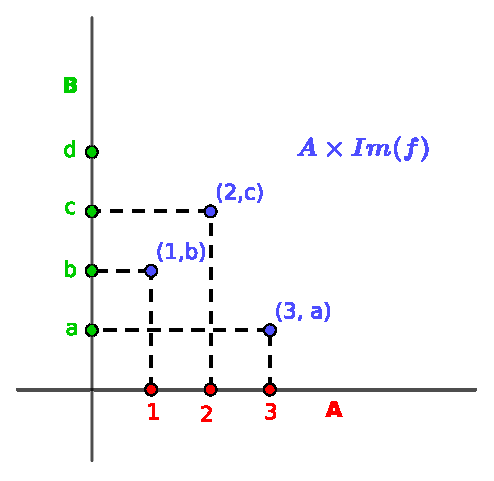
\includegraphics[width=5cm]{./cap_funcao/figs/Grf}}
%     \caption{Gráfico da função $f$}
%   \end{figure}

% \end{exem}


\section{Determinar o maior domínio de uma função real}

Toda função tem que ser composta por domínio, contra-domínio e da expressão da relação. No entanto, é comum uma função real ser apresentada apenas pela expressão da função, sem fazer menção ao seu domínio e contra-domínio. No caso de funções reais, podemos sempre assumir que seu contra-domínio é o conjunto dos números reais $\R$. Porém, o domínio nem sem é todo o conjunto e, assim, precisamos determinar o maior domínio $A\subset \R$ da função que satisfaça a lei de correspondência definida.

\begin{exem}\hfill
    \begin{enumerate}
        \item Para $f(x)=-x$, o maior domínio é $\R$;
        \item Para $f(x)=\frac{1}{x}$, o maior domínio é $\R^{*}$, pois não é possível dividir por zero;
        \item Para $f(x)=\sqrt{x}$, o maior domínio é $\R_{+}$, pois não existe raiz quadrada de número negativo.
    \end{enumerate}
\end{exem}

Note que algumas operações fornecem restrições no domínio. Por enquanto, podemos destacar duas delas:
\begin{itemize}
    \item Divisão por zero: se $f(x)=\dfrac{g(x)}{h(x)}$ então $h(x)\neq 0$;
    \item Raiz de índice par: se $f(x)=\sqrt[par]{g(x)}$ então $g(x)\geq 0$.
\end{itemize}

É possível combinar os dois casos anteriores: se $f(x)=\dfrac{g(x)}{\sqrt[par]{h(x)}}$ então $h(x)> 0$.

\begin{exem}
    Determine o maior domínio da função real $f(x)=\dfrac{1}{x+1}+\sqrt{-x}$.

    A fração fornece a restrição: $x+1= 0$, ou seja, devemos ter $x\neq -1$.

    A raiz quadrada diz que $-x\geq 0$, ou seja, $x\leq 0$.

    Portanto, o maior domínio de $f$ é $A=(-\infty,-1)\cup(-1,0]$.
\end{exem}

% \section{Operações com funções}
% Dadas as funções $f: A \rightarrow \R$, $g: B \rightarrow \R$, se $A \cap B \neq \emptyset$, então $\forall x \in A \cap B$, definimos as seguintes operações entre estas funções:
% \begin{equation*}
% (f + g)(x)= f(x) + g(x); 
% \end{equation*}
% \begin{equation*}
% (f - g)(x)= f(x) - g(x); 
% \end{equation*}
% \begin{equation*}
% (f \cdot g)(x)= f(x) \cdot g(x); 
% \end{equation*}
% \begin{equation*}
%  \left( \frac{f}{g} \right) (x)= \frac{f(x)}{g(x)} ;
% \end{equation*}
% \begin{equation*}
% (k \cdot f)(x)= k \cdot f(x), \text{ para } k \text{ constante} ,
% \end{equation*}

% note que:
% \begin{equation*}
% dom(f+g)= dom(f-g)= dom(f \cdot g)= dom(k \cdot f)= A \cap B ,
% \end{equation*}
% \begin{equation*}
%  dom\left( \frac{f}{g} \right)= \{x \in A \cap B \mid g(x) \neq 0\}. 
% \end{equation*}

\section{Função constante}

A função contante é a função que associa todos os elementos do domínio a um único elemento do contradomínio. Ou seja, dado $a \in \R$ fixo, a função $f$:
\begin{eqnarray*}
 f: \R & \rightarrow & \R \\
 x & \mapsto & a,
\end{eqnarray*}
é uma função constante.

Por exemplo, a função $f:\R\to\R$ tal que $f(x)=2$ é uma função constante. Para construir o gráfico desta função começamos encontrando alguns pontos $(x, y)= (x, f(x))$ do gráfico, o que pode ser feito através da seguinte tabela:

 \begin{table}[H]
 \centering
 \begin{tabular}{|c|c|c|} \hline
 \rowcolor{gray}
  x & f(x) & (x, y)  \\\hline
  -1 & f(-1)= 2 & (-1, 2) \\\hline
   0 & f(0)= 2 & (0, 2)  \\\hline
   1 & f(1)= 2 & (1, 2) \\\hline
 \end{tabular}
\end{table}

Após encontrar os pontos basta marcar os mesmo o plano cartesiano e traçar a curva que liga estes pontos com isso objetos o gráfico da função. Neste caso o gráfico é:
\begin{figure}[H]
 \centering
    \fbox{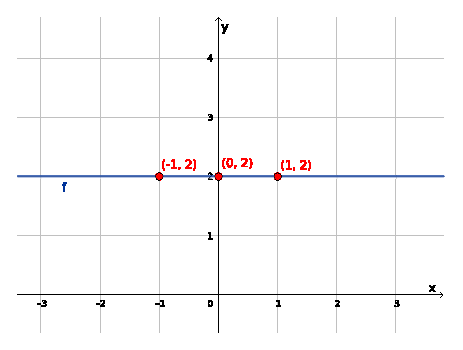
\includegraphics[width=7cm]{./cap_funcao/figs/f(x)=2}}
    \caption{Gráfico da função $f(x)=2$}
  \end{figure}

\section{Função identidade}

A função $Id$:
\begin{eqnarray*}
 Id: \R & \rightarrow & \R \\
 x & \mapsto & x \ ,
\end{eqnarray*}
é chamada \textit{função identidade real}.

Para encontrar alguns pontos $(x, f(x))$ do gráfico desta função, construímos a seguinte tabela:

 \begin{table}[H]
 \centering
 \begin{tabular}{|c|c|c|} \hline
 \rowcolor{gray}
  x & f(x) & (x, y)  \\\hline
  -1 & f(-1)= -1 & (-1, -1) \\\hline
   0 & f(0)= 0 & (0, 0)  \\\hline
   1 & f(1)= 1 & (1, 1) \\\hline
 \end{tabular}
\end{table}

Logo o gráfico da função $Id$ é:
\begin{figure}[H]
 \centering
    \fbox{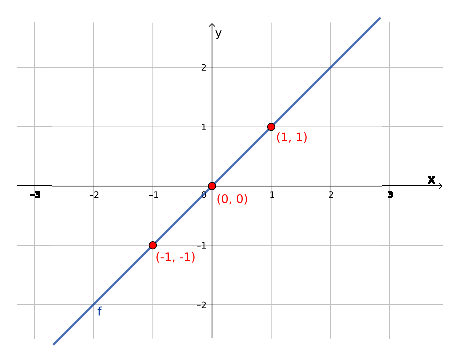
\includegraphics[width=7cm]{./cap_funcao/figs/Id(x)=x}}
    \caption{Gráfico da função $Id(x)=x$}
  \end{figure}


\section{Funções do 1º grau}
 As funções do 1º grau, ou funções afim são funções $f: \R \rightarrow \R$ dadas por:
\begin{equation*}
f(x)= ax + b \ , 
\end{equation*}
para certos $a, b \in \R$ com $a \neq 0$. Note que um caso particular e já conhecido de função de 1º grau é a função identidade, $f(x)= x$, a qual possui $a=1$ e $b=0$.

 Vejamos mais alguns exemplos de funções de 1º grau.

\begin{exem}
 Consideremos as funções $f, g: \R \to \R$ dadas por:
 \begin{enumerate}[a)]
  \item $f(x)= x+2$
  \item $g(x)= x-1$
 \end{enumerate}


 \begin{figure}[H]
   \fbox{\subfigure[$f(x)= x+2$]{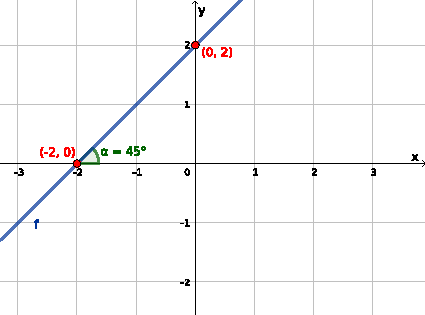
\includegraphics[width=7cm,height=6cm]{./cap_funcao/figs/f(x)=x+2}}}
   \fbox{\subfigure[$g(x)= x-1$]{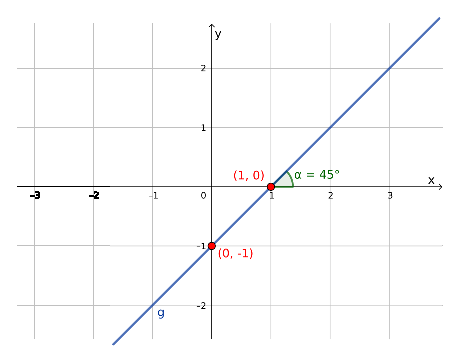
\includegraphics[width=7cm,height=6cm]{./cap_funcao/figs/f(x)=x-1}}}
  \end{figure}
  Note que o que muda na definição destas funções é apenas o coeficiente $b$. Fazendo uma análise comparativa dos gráficos destas funções notamos que os ângulos que as retas formam com o eixo $x$ é o mesmo, portanto as retas são paralelas, porém o ponto de interseção das retas com o eixo $y$, que são os pontos $(0, f(0))$, $(0, g(0))$ muda, ou seja, $f(0) \neq g(0)$. De fato:
\begin{equation*}
f(0)= 0 + 2= 2
\end{equation*}
\begin{equation*}
g(0)= 0 -1 = -1 \ .
\end{equation*}
\end{exem}
  
  No caso geral em que $f(x)=ax+b$, teremos que $f(0)=a0 + b= b$, portanto o gráfico de $f$ irá intersectar o eixo $y$ no ponto $(0,b)$. O coeficiente $b$ é chamado de \textbf{coeficiente linear} da reta/função linear.

\begin{exem}
  Consideremos as funções $f, g: \R \to \R$ dadas por:
 \begin{enumerate}[a)]
  \item $f(x)= 2x$
  \item $g(x)= -2x$
 \end{enumerate}

 \begin{figure}[H]
   \fbox{\subfigure[$f(x)= 2x$]{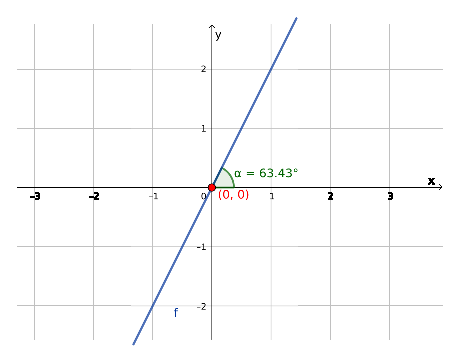
\includegraphics[width=7cm,height=6cm]{./cap_funcao/figs/f(x)=2x}}}
   \fbox{\subfigure[$g(x)= -2x$]{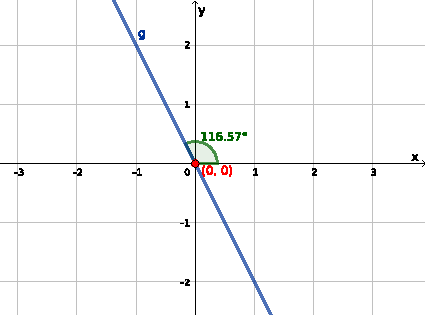
\includegraphics[width=7cm,height=6cm]{./cap_funcao/figs/g(x)=-2x}}}
  \end{figure}
    
  Neste exemplos estamos mudando apenas o coeficiente $a$ das funções, o que está alterando o ângulo que as retas formam com o eixo $x$, ou seja a inclinação das retas em relação ao eixo $x$. Já o ponto de interseção das retas com o eixo $y$ é o mesmo pois $f(0)= g(0)= 0$.
  \end{exem}
  
  O coeficiente $a$ é chamado de \textbf{coeficiente angular} da reta/função linear.

\begin{obs}
 O gráfico de uma função linear $f: \R \to \R$ dada por:
\begin{equation*}
f(x) = ax + b
\end{equation*}
 é uma reta com coeficiente angular $a$ e cuja interseção com o eixo $y$ ocorre no ponto $(0, b)$.
\end{obs}

 Frequentemente a equação da reta é dada pela equação $y=mx+n$, que nada mais é do que uma função de 1º grau, basta considerar $y=f(x)$ o que fazemos no contexto de funções para trabalhar com o gráfico da função.

 \subsection{Coeficiente angular da reta}

  Dados dois pontos $P_0=(x_0, y_0)$, $P_1=(x_1, y_1)$, com $x_0 \neq x_1$, como na figura:

 \begin{figure}[H]
 \centering
    \fbox{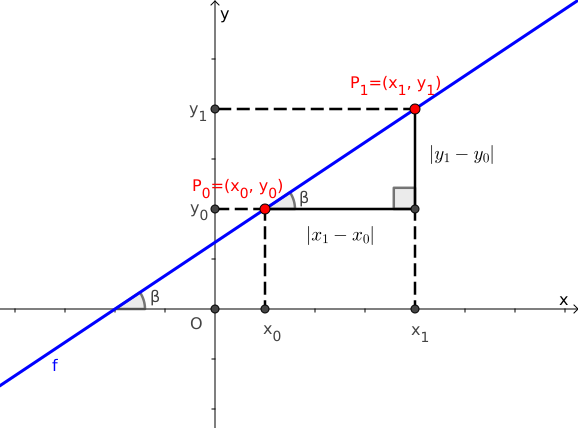
\includegraphics[width=8cm]{./cap_funcao/figs/coefangular}}
    \caption{Coeficiente angular da reta}
  \end{figure}

  O coeficiente angular da reta que passa por estes dois pontos é dado por:
\begin{equation*}
a= \frac{y_1 - y_0}{x_1 - x_0} \ \ \ \text{ ou } \ \ \ a= \frac{y_0 - y_1}{x_0 - x_1} \ .
\end{equation*}

  De fato, dados dois pontos $P_0=(x_0, y_0)$, $P_1=(x_1, y_1)$, com $x_0 \neq x_1$, podemos encontrar a função $f(x)= ax+b$, cujo gráfico passa por estes dois pontos lembrando que ambos devem satisfazer a equação da função assim obtemos:
  \[ \begin{cases}
   y_0= ax_0 + b \\
   y_1= ax_1 + b
  \end{cases} \]
  logo $y_0 - ax_0= b$, substituindo na segunda equação decorre que:
\begin{equation*}
y_1= ax_1 + y_0 - ax_0 \Rightarrow y_1 - y_0= a(x_1 - x_0) \Rightarrow a= \frac{y_1 - y_0}{x_1 - x_0} \ . 
\end{equation*}

  Este sistema linear sempre pode ser usado para encontrar a regra da função linear que passa por dois pontos dados.


  \begin{exem}
  Vamos determinar o coeficiente angular da reta que passa pelos pontos:
   \begin{enumerate}[a)]
    \item $P_0=(0,2)$ e $P_1=(-2,0)$
\begin{equation*}
a= \frac{y_1 - y_0}{x_1 - x_0}= \frac{0 - 2}{-2 - 0}= \frac{-2}{-2}= 1
\end{equation*}
    \item $P_0=(1,2)$ e $P_1=(-1,-2)$
\begin{equation*}
a= \frac{y_1 - y_0}{x_1 - x_0}= \frac{-2 - 2}{-1 - 1}= \frac{-4}{-2}= 2
\end{equation*}
   \end{enumerate}

  \end{exem}

  Quando dados dois pontos $P_0=(x_0, y_0)$, $P_1=(x_1, y_1)$, com $x_0 = x_1$, temos uma reta vertical, cuja equação é $x= a$ para algum $a \in \R$, que não é o gráfico de uma função, por isso não iremos detalhar este caso.

  Dadas duas funções lineares $f(x)=a_1 x + b_1$ e $g(x)= a_2 x + b_2$, tais que $f(x) \neq g(x)$, a partir da análise de seus coeficientes angulares podemos conhecer a posição relativa de seus gráficos. Nesta situação temos dois casos especiais:
  \begin{itemize}
  \item Se $a_1= a_2$ então os gráficos de $f$ e $g$ são retas \textbf{paralelas};
  \item Se $a_1 \cdot a_2= -1$ então os gráficos de $f$ e $g$ são retas \textbf{perpendiculares}.
  \end{itemize}

  \begin{exem}
  Considere as funções $g(x)= -2x+4$, $f(x)= -2x+2$, $h(x)= \frac{-1}{-2}x+ 1,5$, pela análise com coeficientes angulares temos que os gráficos de $g$ e $f$ são retas paralelas e os gráficos $g$ e $h$ são retas perpendiculares, como podemos ver nos seguintes gráficos:
     \begin{figure}[H]
   \fbox{\subfigure[Retas paralelas]{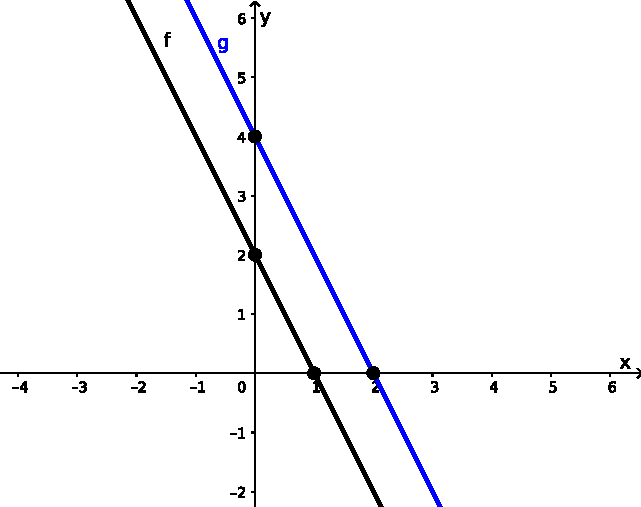
\includegraphics[width=7cm,height=6cm]{./cap_funcao/figs/retasparalelas}}}
   \fbox{\subfigure[Retas perpendiculares]{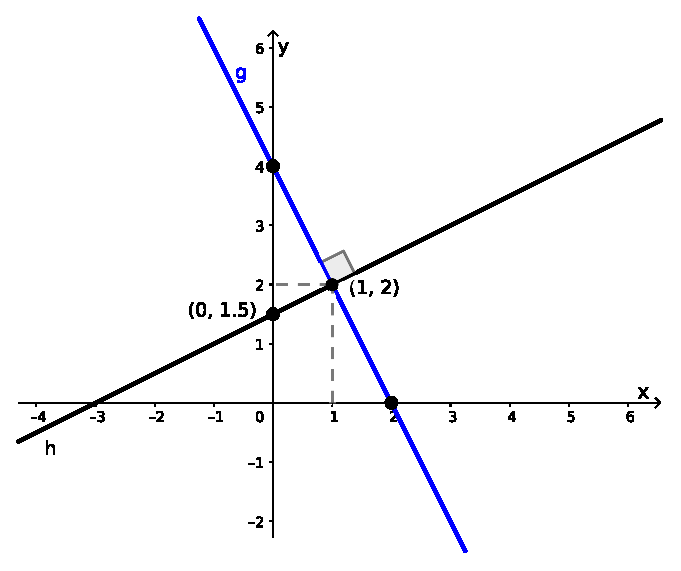
\includegraphics[width=7cm,height=6cm]{./cap_funcao/figs/retasperpendiculares}}}
  \end{figure}
  \end{exem}


 \subsection{Zeros ou raízes das funções afins}

%  \begin{obs}
%  Os zeros ou raízes de uma função $y= f(x)$ são os $x \in Dom(f)$ tais que $f(x)= 0$.
% \end{obs}

 Os zeros de uma função de 1º grau são as raízes da equação $ax+b=0$. Como esta equação é do 1º grau, ela possui uma única raiz, logo a função de 1º grau também possui uma única raiz, que denotaremos por $x'$. Note que o ponto $(x', 0)$ é o ponto de interseção do gráfico da $f$ com o eixo $x$, assim podemos interpretar graficamente as raízes da nossa função como sendo os pontos de interseção do gráfico da função com o eixo das abscissas.

\section{Função (De)crescente}

\begin{obs}
  Sejam $A, B \subset \R$ e uma função real $f: A \rightarrow B$.

  Dizemos que $f$ é uma \textbf{função crescente} em um intervalo $I \subset A$ se, para todo $x, y \in I$,
\begin{equation*}
 x < y \Rightarrow f(x) < f(y).
\end{equation*}

  Dizemos que $f$ é uma \textbf{função decrescente} em um intervalo $I \subset A$ se, para todo $x, y \in I$,
\begin{equation*}
x < y \Rightarrow f(x) > f(y).
\end{equation*}

  Dizemos que $f$ é uma \textbf{função constante} em um intervalo $I \subset A$ se, para todo $x, y \in I$,
\begin{equation*}
x \neq y \Rightarrow f(x) = f(y).
\end{equation*}
\end{obs}

 Seja $f: \R \to \R$ uma função linear dada por $f(x)= ax + b$.

\begin{itemize}
    \item Se \destaque{a > 0} então dados $x_1 < x_2$, temos que:
\begin{equation*}
x_1 < x_2 \Rightarrow ax_1 < ax_2 \Rightarrow ax_1 + b < ax_2 + b \ ,
\end{equation*}
  portanto $f(x_1) < f(x_2)$, neste caso dizemos que $f$ é \textbf{crescente}.

 \item Se \destaque{a < 0} então  dados $x_1 < x_2 \in dom(f)$, temos que:
\begin{equation*}
x_1 < x_2 \Rightarrow ax_1 > ax_2 \Rightarrow ax_1 + b > ax_2 + b \ ,
\end{equation*}
 portanto $f(x_1) > f(x_2)$, neste caso dizemos que $f$ é \textbf{decrescente}.
 \end{itemize}

 Observe que no caso das funções de 1º grau a propriedade de ser crescente ou decrescente é válida em todo o domínio da função, nestes casos dizemos que é uma propriedade global da função.

 \begin{exem}
 Vamos retomar alguns dos nossos exemplos de funções para classificar como crescente, decrescente e constante. Para isso considere $x_1= -2$ e $x_2= 1$, neste caso, $x_1 < x_2$.
  \begin{enumerate}[a)]
   \item Sendo $f(x)= \frac{1}{2}x + 1,5$, temos que
\begin{equation*}
f(x_1)= f(-2)= \frac{1}{2}\cdot (-2) + 1,5= -1 + 1,5= 0,5
\end{equation*}
\begin{equation*}
f(x_2)= f(1)= \frac{1}{2} \cdot 1+\frac{3}{2}= \frac{4}{2}= 2
\end{equation*}
   logo $f(x_1)= 0,5 < 2= f(x_2)$. Portanto $f$ é crescente.
   \item Sendo $f(x)= -2x + 2$, temos que
\begin{equation*}
f(x_1)= f(-2)= -2 \cdot (-2) + 2= 4 + 2= 6
\end{equation*}
\begin{equation*}
f(x_2)= f(1)= -2 \cdot 1 + 2= 0
\end{equation*}
   logo $f(x_1)= 6 > 0 = f(x_2)$. Portanto $f$ é decrescente.
   \item Sendo $f(x)= 2$, temos que
\begin{equation*}
f(x_1)= f(-2)= 2
\end{equation*}
\begin{equation*}
f(x_2)= f(1)= 2
\end{equation*}
   logo $f(x_1)= 2 = 2= f(x_2)$. Portanto $f$ é constante.
  \end{enumerate}
  Como já mostramos acima que para as funções lineares esta propriedade é global, para fazer esta classificação é suficiente testar dois valores de $x$ como fizemos acima.

 \end{exem}

\begin{secExercicios}
    \begin{exer}
        Dada a função $f:\R\to\R$ com $f(x)=x^2-3x+1$, determine:
        \begin{enumerate}[a)]
            \begin{multicols}{3}
                \item $f(-2)$
                \item $f(\sqrt{2})$
                \item $f\left(-\frac{1}{2}\right)$
            \end{multicols}
        \end{enumerate}
    \end{exer}

    \begin{exer}
        Dado o conjunto $A=\{-2,-1,0,1,2\}$, determine a imagem da função $f:A\to\R$ para cada uma das seguintes expressões:
        \begin{enumerate}[a)]
            \item $f(x)=2x$
            \item $f(x)=x^2-1$
            \item $f(x)=x^3$
        \end{enumerate}
    \end{exer}

    \begin{exer}
        Considere as funções $f(x)=-5x+2$ e $g(x)=\frac{2}{3}x+a$. Calcule o valor de $a$ de modo que $f(1)-g(1)=\frac{7}{2}$.
    \end{exer}

    \begin{exer}
        Determine o maoir domínio de cada uma das seguintes funções reais:
        \begin{enumerate}[a)]
            \item $f(x)=4x+5$
            \item $f(x)=\dfrac{1}{-3x+12}$
            \item $f(x)=\sqrt{x+9}$
            \item $f(x)=\sqrt{x-1}+\sqrt{1-x}$
            \item $f(x)=\dfrac{x}{x^2-x-6}+\dfrac{1}{x+4}$
            \item $f(x)= \dfrac{1}{\sqrt[3]{x}}$
            \item $f(x)=\sqrt{x-2}+\dfrac{x+1}{x-3}$
            \item $f(x)=\dfrac{x+1}{\sqrt{x^2-4}}$
            \item $f(x)=\dfrac{\sqrt{x+1}}{x^3} + \dfrac{2x}{\sqrt{x+4}}$
        \end{enumerate}
    \end{exer}
    
    \begin{exer}
        Dada a função $f(x)=-x^2+2x$, simplifique:
        \begin{enumerate}[a)]
        \begin{multicols}{2}
            \item $\dfrac{f(x)-f(1)}{x-1}$
            \item $\dfrac{f(x+h)-f(x)}{h}$
        \end{multicols}
        \end{enumerate}
    \end{exer}

    \begin{exer}
        Simplifique $\frac{f(x)-f(p)}{x-p}$, com $x\neq p$, para cada uma das funções a seguir:
        \begin{enumerate}[a)]
            \item $f(x)=2x+1$ para $p=0$.
            \item $f(x)=x^2$ para $p=1$.
            \item $f(x)=x^3$ para $p=2$.
            \item $f(x)=\frac{1}{x}$ para $p=1$.
            \item $f(x)=-x+4$ para $p$ qualquer.
            \item $f(x)=x^2$ para $p$ qualquer.
        \end{enumerate}
    \end{exer}

    \begin{exer}
        Determine o maior domínio, imagem e esboce o gráfico de cada umas das funções a seguir:
        \begin{enumerate}[a)]
        \begin{multicols}{2}
            \item $f(x)=\frac{5}{4}$
            \item $f(x)=-3x$
            \item $f(x)=2x-6$
            \item $f(x)=\frac{1}{2}x +2$
        \end{multicols}
        \end{enumerate}
    \end{exer}

    \begin{exer}
        Estude o sinal das seguintes funções:
        \begin{enumerate}[a)]
            \item $f(x)=4x-5$
            \item $f(x)=2-3x$
            \item $f(x)=\frac{x}{3}-1$
            \item $f(x)=2x+5$
            \item $f(x)=-5x+1$
        \end{enumerate}
    \end{exer}

    \begin{exer}
        Considere as funções reais dadas por $f(x)=8-x$ e $g(x)=3x$. Calcule o ponto de interseção do gráfico detas funções.
    \end{exer}

    \begin{exer}
        Seja $f$ uma função afim tal que $f(3)=5$ e $f(-2)=-5$. Calcule $f\left(\frac{1}{2}\right)$.
    \end{exer}

    \begin{exer}
        Considere a função real $f(x)$ tal que $f(1)=43$ e $f(x+1)=2f(x)-15$. Determine o valor de $f(0)$.
    \end{exer}

    \begin{exer} Determine a expressão de cada uma das funções para cada um dos gráficos abaixo
        \begin{enumerate}[a)]
            \item 
            \begin{tikzpicture}[scale=0.7]
            \tkzInit[xmin=-3, xmax=3, xstep=1, ymin=-1,ymax=4]
                %\tkzDrawXY
                \tkzAxeXY
                
                \tkzFct[thick,red]{2*x+3}
            
                %\tkzDefPointByFct[ref=A, with=a](-1)
                \tkzDefPoint(-1,1){A}
                \tkzDefPoint(0,3){B}
                \tkzPointShowCoord(A)
                \tkzDrawPoint[fill=red, size=3](A)
                \tkzDrawPoint[fill=red, size=3](B)
                
            \end{tikzpicture}

            \item 
            \begin{tikzpicture}[scale=0.7]
            \tkzInit[xmin=-3, xmax=3, xstep=1, ymin=-1,ymax=3]
                %\tkzDrawXY
                \tkzAxeXY
                
                \tkzFct[thick,red]{-0.5*x+1}
            
                %\tkzDefPointByFct[ref=A, with=a](-1)
                \tkzDefPoint(0,1){A}
                \tkzDefPoint(2,0){B}
                %\tkzPointShowCoord(A)
                \tkzDrawPoint[fill=red, size=3](A)
                \tkzDrawPoint[fill=red, size=3](B)
                
            \end{tikzpicture}

            \item 
            \begin{tikzpicture}[scale=0.7]
            \tkzInit[xmin=-3, xmax=3, xstep=1, ymin=-2,ymax=1]
                %\tkzDrawXY
                \tkzAxeXY
                
                \tkzFct[thick,red]{0.666*x-1}
            
                %\tkzDefPointByFct[ref=A, with=a](-1)
                \tkzDefPoint(3,1){A}
                \tkzDefPoint(0,-1){B}
                \tkzPointShowCoord(A)
                \tkzDrawPoint[fill=red, size=3](A)
                \tkzDrawPoint[fill=red, size=3](B)
                
            \end{tikzpicture}

            \item 
            \begin{tikzpicture}[scale=0.7]
            \tkzInit[xmin=-2, xmax=4, xstep=1, ymin=-4,ymax=1]
                %\tkzDrawXY
                \tkzAxeXY
                
                \tkzFct[thick,red]{-0.75*x}
            
                %\tkzDefPointByFct[ref=A, with=a](-1)
                \tkzDefPoint(4,-3){A}
                \tkzDefPoint(0,0){B}
                \tkzPointShowCoord(A)
                \tkzDrawPoint[fill=red, size=3](A)
                \tkzDrawPoint[fill=red, size=3](B)
            \end{tikzpicture}
        \end{enumerate}
    \end{exer}

    \begin{exer}
        Seja $f(2x+7)=-4x+9$. Determine o valor de $f(-5)$.
    \end{exer}

    \begin{exer}
        Determine os possíveis valores de $p$ para que a função $f(x)=(2p+3)x+2$ seja decrescente.
    \end{exer}

    \begin{exer}
        Determine o valor de $p$ de modo que o gráfico da função $f(x)=2x+p+3$ passe pelo ponto $(1,2)$.
    \end{exer}
    
    \begin{exer}
        Dadas as funções $f$ e $g$ cujas expressões são $f(x)=ax+4$ e $g(x)=bx+1$, calcule $a$ e $b$ de modo que os gráficos das funções interseptem-se no ponto $(1,6)$.
    \end{exer}
    
    \begin{exer}
 Uma bolsa de valores tinha um preço de R\$ $42,00$ quando sofreu uma queda de R\$$2,50$ por dia, durante $5$ dias seguidos.
  \begin{enumerate}[a)]
  \item Qual é a função que representa a queda do valor dessa ação em função do dia?
  \item Represente, no plano cartesiano, os pontos correspondentes a esses $5$ dias e o segmento de reta que passa por esses pontos.
  \end{enumerate}
  \end{exer}
  \begin{resp}
    a) $f(x)= 42 - 2,50 x$; b) a cargo do leitor;
  \end{resp}
  
  \begin{exer}
  Um táxi, realizando uma corrida, cobra uma taxa fixa denominada bandeira de R\$$3,50$ e R\$$0,80$ por quilômetro rodado.
  Com base nesses dados, determine:
  \begin{enumerate}[a)]
  \item A função que representa o valor pago por uma corrida de $x$ quilômetros.
  \item Quantos quilômetros foram rodados se a conta foi de R\$ $17,10$.
  \end{enumerate}
  \end{exer}
  \begin{resp}
    a) $f(x)= 3,50 + 0,80 x$; b) $x= 17 Km$;
  \end{resp}
  
  \begin{exer}
  Para cercar um terreno, tem-se duas opções:
  1ª) Taxa de entrega no local R\$ $100,00$ e R\$$12,00$ o metro linear de cerca.
  2ª) Taxa de entrega no local R\$ $80,00$ e R\$ $15,00$ o metro linear de cerca.
  \begin{enumerate}[a)]
  \item Represente o custo de cada opção para $x$ metros de cerca.
  \item Qual das duas opções é mais vantajosa para $140$m de perímetro.
  \end{enumerate}
  \end{exer}
  \begin{resp}
    a) 1ª opção: $f(x)= 100 + 12x$, 2ª opção: $f(x)= 80+15x$; b) 1ª opção; 
  \end{resp}
  
%   \begin{exer}
%   No Brasil, o sistema de numeração de sapatos ou tênis é baseado na fórmula $N(p)= \frac{5p + 28}{4}$, que indica o valor aproximado do número do calçado $N$ em função do comprimento $p$, em centímetros do pé da pessoa. Determine o número do sapato ou tênis que uma pessoa deve comprar se, ao medir o comprimento de seu pé obteve:
%   \begin{enumerate}[a)]
%   \item $22,8$ cm
%   \item $24$ cm
%   \item $26,4$ cm
%   \end{enumerate}
%   \end{exer}
%   \begin{resp}
%     a) $35,5$; b) $37$; c) $40$;
% %    \par\noindent\rule{\columnwidth}{0.4pt}
%   \end{resp}
\end{secExercicios}

%\subsection*{Respostas}

%\shipoutAnswer

 




%\subsection*{Respostas}

%\shipoutAnswer



%\subsection*{Respostas}

%\shipoutAnswer

 
% \setcounter{chapter}{10} 
\chapter{Funções do 2º grau}
As funções do 2º grau ou função quadrática são funções reais $f: \R \rightarrow \R$ dadas por:
\begin{equation*}
f(x)= ax^2 + bx + c \ ,
\end{equation*}
com $a, b, c \in \R$ e $a \neq 0$. 

O gráfico de uma função de 2º grau é um parábola. Nosso objetivo é extrair alguns elementos da função que possam nos orientar para representar seu gráfico com precisão.

Para determinar o gráfico, precisamos determinar quatro elementos importantes das parábolas que podem ser extraídas da função:

\begin{itemize}
    \item Concavidade: o gráfico da função de 2º grau tem concavidade voltada \textbf{para cima} quando \destaque{a > 0}, e concavidade voltada \textbf{para baixo} quando \destaque{a < 0}.
    
    \item Raízes: Os \textbf{zeros} ou \textbf{raízes} das funções de 2º grau $f$, quando existem, são os elementos $x$ de seu domínio tais que $ax^2+bx+c=0$. Por ser esta uma equação do 2º grau temos três situações a considerar, dependendo do valor de $\Delta=b^2-4ac$

 Se \destaque{\Delta < 0} a função $f$ não possui raízes reais;

 Se \destaque{\Delta = 0} a função $f$ possui uma única raiz real;

 Se \destaque{\Delta > 0} a função $f$ possui duas raízes reais distintas, que podem ser calculadas resolvendo a equação de 2º grau através da fórmula para equações de 2º grau.

 Por definição, os zeros da função $f(x)= ax^2+bx+c$, são as raízes da equação $ax^2+bx+c=0$, já que estes são os valores de $x$ para os quais $f(x)=0$. Graficamente, quando estas funções possuem zeros eles são exatamente os pontos de interseção do gráfico da $f$ com o eixo $x$.
 
    \item Interseção com o eixo $y$: esta inteseção ocorre quando $x=0$, ou seja, em $f(0)=c$.
    
    \item Vértice: a função do 2º grau possui um vértice dado pela seguinte equação:
\begin{equation*}
(x_V,y_V)= \left(\frac{- b}{2a}, \frac{- \Delta}{4a} \right).
\end{equation*}

 No caso em que $a > 0$, o vértice do gráfico da função de 2º grau é um ponto de mínimo da função.

 No caso em que $a < 0$, o vértice do gráfico da função de 2º grau é um ponto de máximo da função.
\end{itemize}
 
 \begin{exem}
 Considere a função $f(x)= x^2+x+1$. Observamos que:
 \begin{itemize}
     \item Esta função tem concavidade para cima pois $a=1$;
     \item A função $f$ não possui zeros pois $\Delta=-3$;
     \item Intersecta o eixo $y$ no ponto $(0,1)$;
     \item O vértice de $f$ é o ponto $(-\frac{1}{2}, \frac{3}{4})$.
 \end{itemize}

 % \begin{figure}[H]
 %  \centering
 %  \fbox{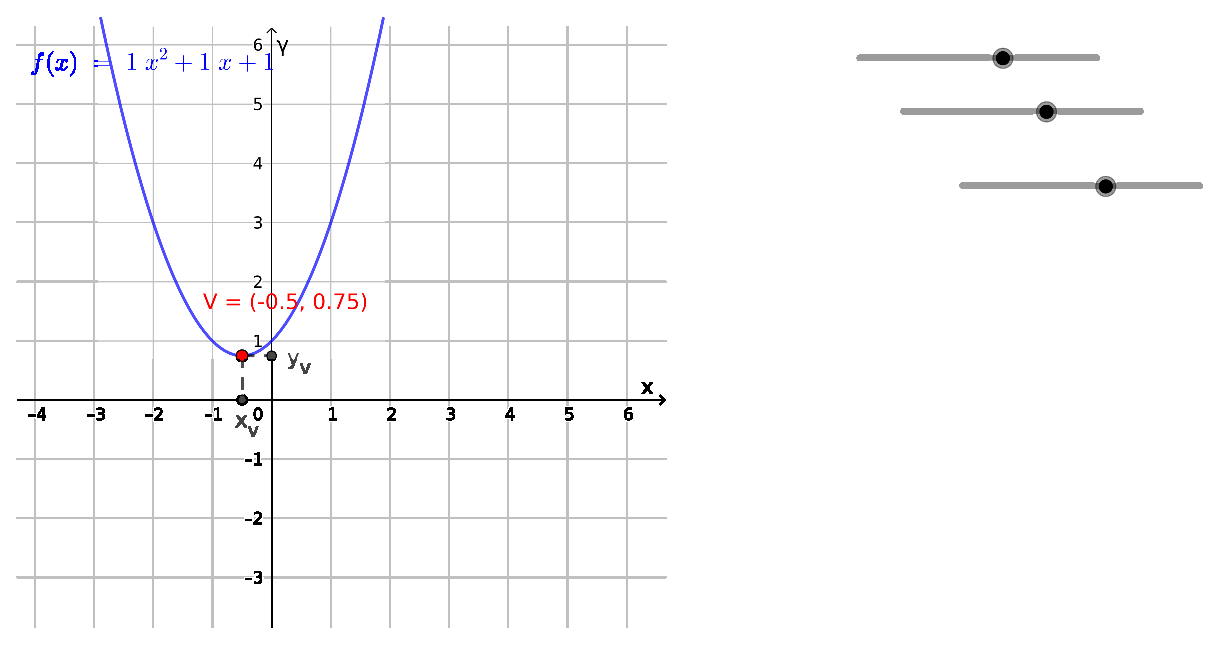
\includegraphics[height=5cm]{./cap_funcao/figs/f1}}
 %   \caption{Gráfico da função $f(x)= x^2+x+1$}
 %  \end{figure}

  \begin{center}
  \begin{tikzpicture}[scale=1]
    \tkzInit[xmin=-3, xmax=3, xstep=1, ymin=-1,ymax=4]
        %\tkzDrawXY
        \tkzAxeXY[fill=black!5]
        
        \tkzFct[thick,red]{x**2+x+1}
    
        %\tkzDefPointByFct[ref=A, with=a](-1)
        \tkzDefPoint(0,1){A}
        \tkzDefPoint(-0.5,0.75){B}
        \tkzPointShowCoord(B)
        \tkzDrawPoint[fill=red, size=3](A)
        \tkzDrawPoint[fill=red, size=3](B)
        
    \end{tikzpicture}
\end{center}
  
 \end{exem}
 
  \begin{exem}
 Considere a função $f(x)= x^2-4x+4$.
  %  \begin{figure}[H]
  % \centering
  % \fbox{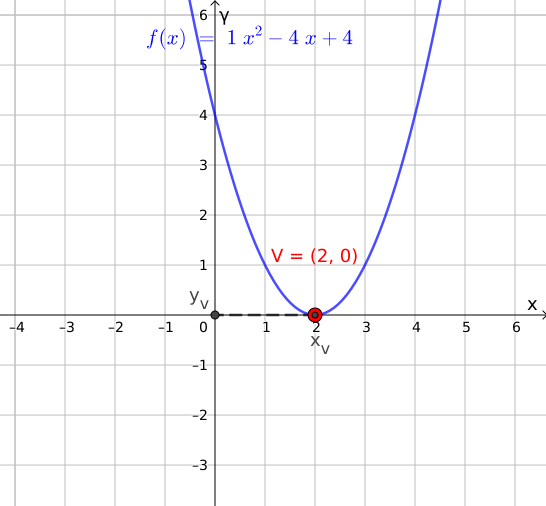
\includegraphics[height=5cm]{./cap_funcao/figs/f2}}
  %  \caption{Gráfico da função $f(x)= x^2-4x+4$}
  % \end{figure}

\begin{itemize}
    \item Esta função tem concavidade para cima;
    \item O zero de $f$ é $S= \{2\}$;
    \item Intersecta o eixo $y$ no ponto $(0,4)$;
    \item O vértice de $f$ é o ponto $(2, 0)$.
\end{itemize}

\begin{center}
  \begin{tikzpicture}[scale=1]
    \tkzInit[xmin=-1, xmax=5, xstep=1, ymin=-1,ymax=5]
        %\tkzDrawXY
        \tkzAxeXY[fill=black!5]
        
        \tkzFct[thick,red]{x**2-4*x+4}
    
        %\tkzDefPointByFct[ref=A, with=a](-1)
        \tkzDefPoint(0,4){A}
        \tkzDefPoint(2,0){B}
        %\tkzPointShowCoord(A)
        \tkzDrawPoint[fill=red, size=3](A)
        \tkzDrawPoint[fill=red, size=3](B)
        
    \end{tikzpicture}
\end{center}
 \end{exem}
 
\begin{exem}
 Considere a função $f(x)= x^2-x-2$.

 \begin{itemize}
    \item Esta função tem concavidade para cima;
    \item As raízes de $f$ são $-1$ e $2$;
    \item Intersecta o eixo $y$ no ponto $(0,-2)$;
    \item O vértice de $f$ é o ponto $(\frac{1}{2}, -\frac{9}{4})$.
\end{itemize}

\begin{center}
  \begin{tikzpicture}[scale=1]
    \tkzInit[xmin=-3, xmax=3, xstep=1, ymin=-3,ymax=3]
        %\tkzDrawXY
        \tkzAxeXY[fill=black!5]
        
        \tkzFct[thick,red]{x**2-x-2}
    
        %\tkzDefPointByFct[ref=A, with=a](-1)
        \tkzDefPoint(0,-2){A}
        \tkzDefPoint(0.5,-2.25){B}
        \tkzPointShowCoord(B)
        \tkzDrawPoint[fill=red, size=3](A)
        \tkzDrawPoint[fill=red, size=3](B)
        
    \end{tikzpicture}
\end{center}
%    \begin{figure}[H]
%   \centering
%   \fbox{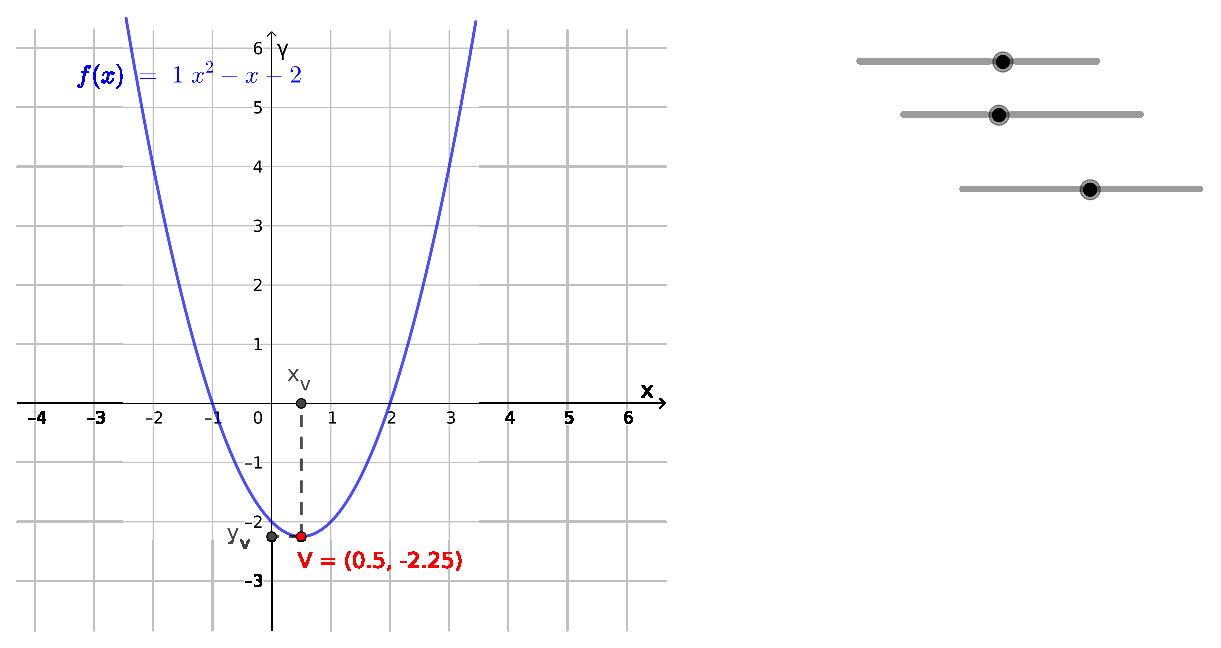
\includegraphics[height=5cm]{./cap_funcao/figs/f3}}
%    \caption{Gráfico da função $f(x)= x^2-x-2$}
%   \end{figure}
%  Observamos que:
%  \begin{enumerate}
% \item [a)] Os zeros de $f$ são $S= \{-1, 2\}$.
% \item [b)] O vértice de $f$ é o ponto $V= (0,5, -2,25)$.
% \item [c)] Esta função tem concavidade para cima.
% \item [d)] O vértice desta função é ponto de mínimo.
% \item [e)] A função é crescente no intervalo $(0,5, \infty)$.
% \item [f)] A função é decrescente no intervalo $(- \infty, 0,5)$.
% \end{enumerate}
\end{exem}

\begin{exem}
 Considere a função $f(x)= -x^2-x-2$.

 \begin{itemize}
    \item Esta função tem concavidade para baixo;
    \item A função $f$ não tem raiz real;
    \item Intersecta o eixo $y$ no ponto $(0,-2)$;
    \item O vértice de $f$ é o ponto $(-\frac{1}{2}, -\frac{7}{4})$.
\end{itemize}

\begin{center}
  \begin{tikzpicture}[scale=1]
    \tkzInit[xmin=-2, xmax=2, xstep=1, ymin=-4,ymax=1]
        %\tkzDrawXY
        \tkzAxeXY[fill=black!5]
        
        \tkzFct[thick,red]{-x**2-x-2}
    
        %\tkzDefPointByFct[ref=A, with=a](-1)
        \tkzDefPoint(0,-2){A}
        \tkzDefPoint(-0.5,-1.75){B}
        \tkzPointShowCoord(B)
        \tkzDrawPoint[fill=red, size=3](A)
        \tkzDrawPoint[fill=red, size=3](B)
        
    \end{tikzpicture}
\end{center}

%    \begin{figure}[H]
%   \centering
%   \fbox{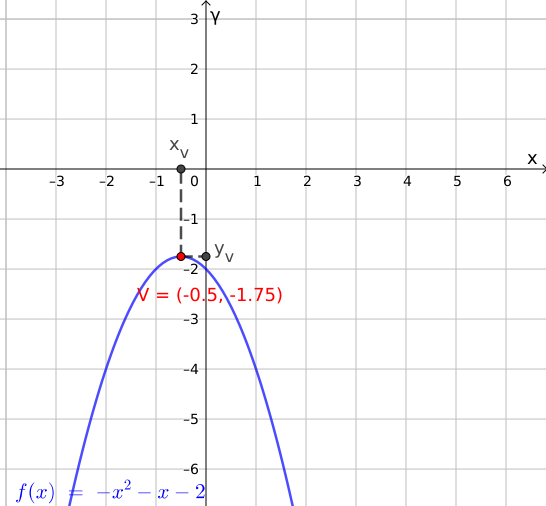
\includegraphics[height=5cm]{./cap_funcao/figs/f4}}
%    \caption{Gráfico da função $f(x)= -x^2-x-2$}
%   \end{figure}
%  Observamos que:
%  \begin{enumerate}
% \item [a)] A função $f$ não possui zeros.
% \item [b)] O vértice de $f$ é o ponto $V= (-0,5, -1,75)$.
% \item [c)] Esta função tem concavidade para baixo.
% \item [d)] O vértice desta função é ponto de máximo.
% \item [e)] A função é crescente no intervalo $(- \infty, -0,5)$.
% \item [f)] A função é decrescente no intervalo $(-0,5, \infty)$.
% \end{enumerate}
\end{exem}

\begin{exem}
 Considere a função $f(x)= -x^2+6x-9$.

 \begin{itemize}
    \item Esta função tem concavidade para baixo;
    \item O zero de $f$ é $S= \{3\}$;
    \item Intersecta o eixo $y$ no ponto $(0,-9)$;
    \item O vértice de $f$ é o ponto $(3, 0)$.
\end{itemize}

\begin{center}
  \begin{tikzpicture}[scale=0.8]
    \tkzInit[xmin=-1, xmax=6, ymin=-9,ymax=1]
        %\tkzDrawXY
        \tkzAxeXY[fill=black!5]
        
        \tkzFct[thick,red,domain=0:6]{-x**2+6*x-9}
    
        %\tkzDefPointByFct[ref=A, with=a](-1)
        \tkzDefPoint(0,-9){A}
        \tkzDefPoint(3,0){B}
        %\tkzPointShowCoord(A)
        \tkzDrawPoint[fill=red, size=3](A)
        \tkzDrawPoint[fill=red, size=3](B)
        
    \end{tikzpicture}
\end{center}
%    \begin{figure}[H]
%   \centering
%   \fbox{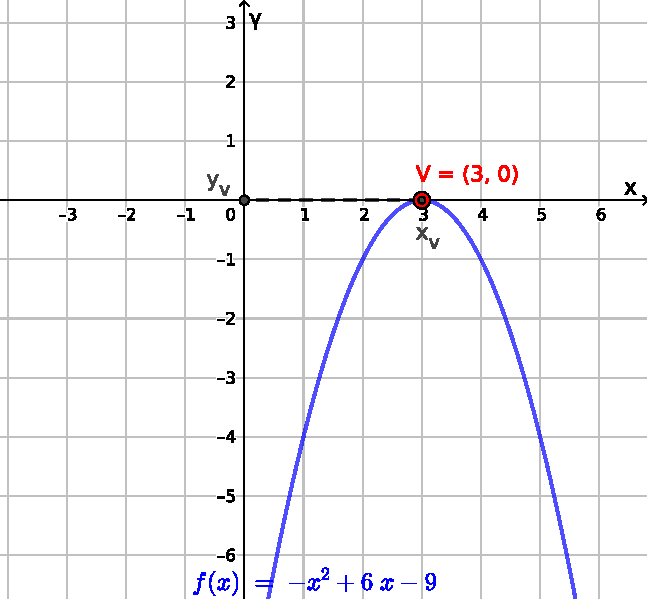
\includegraphics[height=5cm]{./cap_funcao/figs/f5}}
%    \caption{Gráfico da função $f(x)= -x^2+6x-9$}
%   \end{figure}
%  Observamos que:
%  \begin{enumerate}
% \item [a)] O zero de $f$ é $S= \{3\}$.
% \item [b)] O vértice de $f$ é o ponto $V= (3, 0)$.
% \item [c)] Esta função tem concavidade para baixo.
% \item [d)] O vértice desta função é ponto de máximo.
% \item [e)] A função é crescente no intervalo $(-\infty, 3)$.
% \item [f)] A função é decrescente no intervalo $(3, \infty)$.
% \end{enumerate}
\end{exem}

\begin{exem}
 Considere a função $f(x)= -x^2+x+2$.

 \begin{itemize}
    \item Esta função tem concavidade para baixo;
    \item As raízes de $f$ são $-1$ e $2$;
    \item Intersecta o eixo $y$ no ponto $(0,2)$;
    \item O vértice de $f$ é o ponto $(\frac{1}{2}, \frac{9}{4})$.
\end{itemize}

\begin{center}
  \begin{tikzpicture}[scale=1]
    \tkzInit[xmin=-3, xmax=3, xstep=1, ymin=-3,ymax=3]
        %\tkzDrawXY
        \tkzAxeXY[fill=black!5]
        
        \tkzFct[thick,red]{-x**2+x+2}
    
        %\tkzDefPointByFct[ref=A, with=a](-1)
        \tkzDefPoint(0,2){A}
        \tkzDefPoint(0.5,2.25){B}
        \tkzPointShowCoord(B)
        \tkzDrawPoint[fill=red, size=3](A)
        \tkzDrawPoint[fill=red, size=3](B)
        
    \end{tikzpicture}
\end{center}

%    \begin{figure}[H]
%   \centering
%   \fbox{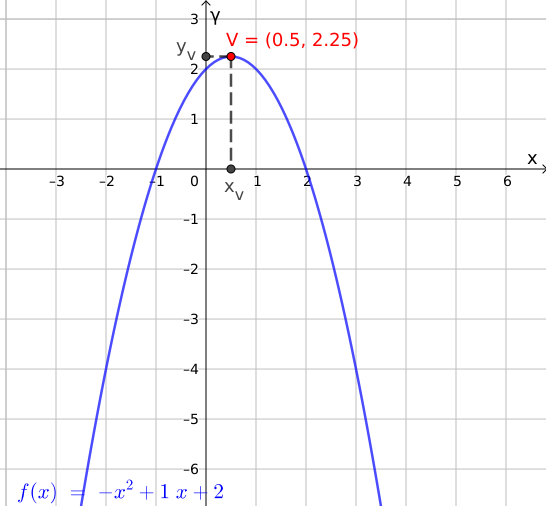
\includegraphics[height=5cm]{./cap_funcao/figs/f6}}
%    \caption{Gráfico da função $f(x)= -x^2+x+2$}
%   \end{figure}
%  Observamos que:
%  \begin{enumerate}
% \item [a)] Os zeros de $f$ são $S= \{-1, 2\}$.
% \item [b)] O vértice de $f$ é o ponto $V= (0,5, 2,25)$.
% \item [c)] Esta função tem concavidade para baixo.
% \item [d)] O vértice desta função é ponto de máximo.
% \item [e)] A função é crescente no intervalo $(-\infty, 0,5)$.
% \item [f)] A função é decrescente no intervalo $(0,5, \infty)$.
% \end{enumerate}
\end{exem}

% \begin{exem}
% Considere a função $f(x)= x^2 - 2x - 3$, determine:
% \begin{enumerate}
% \item [a)] Os zeros de $f$.
% \item [b)] O vértice de $f$.
% \item [c)] Esta função tem concavidade para cima ou para baixo?
% \item [d)] O vértice desta função é ponto de máximo ou mínimo?
% \item [e)] Qual o intervalo no qual a função é crescente?
% \item [f)] Qual o intervalo no qual a função é decrescente?
% \end{enumerate}
%   \begin{figure}[H]
%   \centering
%   \fbox{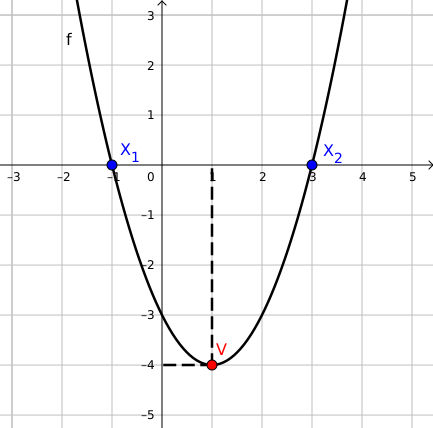
\includegraphics[height=5cm]{./cap_funcao/figs/funcao2grauexem1}}
%    \caption{Gráfico da função $f(x)= x^2 - 2x - 3$}
%   \end{figure}
% \end{exem}

% \begin{resol}
% \begin{enumerate}
% \item [a)] Os zeros de $f$ são $S= \{-1, 3\}$.
% \item [b)] O vértice de $f$ é o ponto $V= (1, -4)$.
% \item [c)] Esta função tem concavidade para cima.
% \item [d)] O vértice desta função é ponto de mínimo.
% \item [e)] A função é crescente no intervalo $(1, \infty)$.
% \item [f)] A função é decrescente no intervalo $(- \infty, 1)$.
% \end{enumerate}
% \end{resol}

% \begin{exem}
% Considere a função $f(x)= -x^2 + 2x + 8$, determine:
% \begin{enumerate}
% \item [a)] Os zeros de $f$.
% \item [b)] O vértice de $f$.
% \item [c)] Esta função tem concavidade para cima ou para baixo?
% \item [d)] O vértice desta função é ponto de máximo ou mínimo?
% \item [e)] Qual o intervalo no qual a função é crescente?
% \item [f)] Qual o intervalo no qual a função é decrescente?
% \end{enumerate}
%   \begin{figure}[H]
%   \centering
%   \fbox{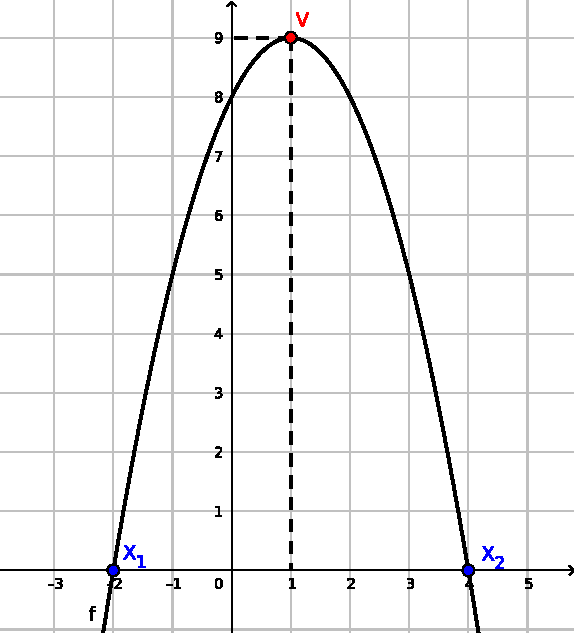
\includegraphics[height=6cm]{./cap_funcao/figs/funcao2grauexem2}}
%    \caption{Gráfico da função $f(x)= -x^2 + 2x + 8$}
%   \end{figure}
% \end{exem}

% \begin{resol}
% \begin{enumerate}
% \item [a)] Os zeros de $f$ são $S= \{-2, 4\}$.
% \item [b)] O vértice de $f$ é o ponto $V= (1,9)$.
% \item [c)] Esta função tem concavidade voltada para baixo.
% \item [d)] O vértice desta função é ponto de máximo.
% \item [e)] A função é crescente no intervalo $(-\infty, 1)$.
% \item [f)] A função é decrescente no intervalo $(1, \infty)$.
% \end{enumerate}
% \end{resol}

\section{Máximos e mínimos da função de 2º grau}

    Seja $f:A\to \R$ uma função real.
\begin{itemize}
    \item Dizemos que $x_M\in A$ é ponto de máximo se $f(x_M)\geqslant f(x)$ para todo $x\in A$.

    \item Dizemos que $x_m\in A$ é ponto de mínimo se $f(x_m)\leqslant f(x)$ para todo $x\in A$.
\end{itemize}

\begin{teo}
    A função quadrática $f(x)=ax^2+bx+c$ admite um ponto de máximo $x_M$ se, e somente se, $a<0$.
\end{teo}

\begin{teo}
    A função quadrática $f(x)=ax^2+bx+c$ admite um ponto de mínimo $x_m$ se, e somente se, $a>0$.
\end{teo}

Com isto podemos determinar a imagem da função de 2º grau com domínio $\R$:
\begin{itemize}
    \item Se $a>0$ então a $\mathrm{Im}(f)=\left[y_V,+\infty)=[-\frac{\Delta}{4a},+\infty\right)$;
    \item Se $a<0$ então a $\mathrm{Im}(f)=\left(-\infty, y_V]=(-\infty,-\frac{\Delta}{4a}\right]$.
\end{itemize}

\begin{secExercicios}

\begin{exer}
    Esboce o gráfico das seguintes funções quadráticas $f:\R\to\R$:

    \begin{enumerate}[a)]
        \item $f(x)=x^2-3x+2$
        \item $f(x)=2x^2+3$
        \item $f(x)=-x^2+2x$
        \item $f(x)=-4x^2+4x-1$
        \item $f(x)=x^2-4$
        \item $f(x)=-x^2+4$
        \item $f(x)=x^2+2x+2$
        \item $f(x)=-x^2-4x-5$
    \end{enumerate}
\end{exer}

\begin{exer}
    Dadas as funções $f(x)=x^2-2x-3$, $g(x)=x^2-2x+1$ e $h(x)=x^2-2x+2$:
    \begin{enumerate}[a)]
        \item Obtenha os valores reais de $x$ tais que $f(x)=0$, $g(x)=0$ e $h(x)=0$.
        \item Dê o vértice de cada uma das parábolas;
        \item Esboce no mesmo sistema cartesiano os gráficos de $f$, $g$ e $h$.
    \end{enumerate}
\end{exer}

\begin{exer}
    Qual é o conjunto imagem de cada uma das funções?
    \begin{enumerate}[a)]
        \item $f(x)=-2x^2+4x-3$
        \item $f(x)=3x^2-5x+1$
    \end{enumerate}
\end{exer}

\begin{exer}
    Uma bola é lançada ao ar. Suponha que sua altura $h$, em metros, $t$ segundos após o lançamento, seja $h=-t^2+4t+6$. Determine:
    \begin{enumerate}[a)]
        \item o instante em que a bola atinge a sua altura máxima;
        \item a altura máxima atingida pela bola;
        \item quantos segundos depois do lançamento ela toca o solo.
    \end{enumerate}
\end{exer}

\begin{exer}
    Encontre a expressão da função quadrática $f:\R\to\R$ para cada um dos gráficos abaixo, justificando sua resposta:
    \begin{center}
        \begin{tikzpicture}[scale=1]
            \tkzInit[xmin=-1, xmax=5, xstep=1, ymin=-1,ymax=2]
            %\tkzDrawXY
            \tkzAxeXY
            
            \tkzFct[thick,red]{0.25*x**2-x+1}
        
            %\tkzDefPointByFct[ref=A, with=a](-1)
            \tkzDefPoint(0,1){A}
            \tkzDefPoint(2,0){B}
            %\tkzPointShowCoord(B)
            \tkzDrawPoint[fill=red, size=3](A)
            \tkzDrawPoint[fill=red, size=3](B)
        \end{tikzpicture}
    \end{center}

    \begin{center}
        \begin{tikzpicture}[scale=1]
            \tkzInit[xmin=-1, xmax=5, xstep=1, ymin=-4,ymax=1]
            %\tkzDrawXY
            \tkzAxeXY
            
            \tkzFct[thick,red]{-0.25*x**2+x-3}
        
            %\tkzDefPointByFct[ref=A, with=a](-1)
            \tkzDefPoint(0,-3){A}
            \tkzDefPoint(2,-2){B}
            \tkzPointShowCoord(B)
            \tkzDrawPoint[fill=red, size=3](A)
            \tkzDrawPoint[fill=red, size=3](B)
        \end{tikzpicture}
    \end{center}

    \begin{center}
        \begin{tikzpicture}[scale=1]
            \tkzInit[xmin=-3, xmax=1, xstep=1, ymin=-3,ymax=1]
            %\tkzDrawXY
            \tkzAxeXY
            
            \tkzFct[thick,red]{2*x**2+4*x-1}
        
            %\tkzDefPointByFct[ref=A, with=a](-1)
            \tkzDefPoint(0,-1){A}
            \tkzDefPoint(-1,-3){B}
            \tkzPointShowCoord(B)
            \tkzDrawPoint[fill=red, size=3](A)
            \tkzDrawPoint[fill=red, size=3](B)
        \end{tikzpicture}
    \end{center}
    
    \begin{center}
        \begin{tikzpicture}[scale=1]
            \tkzInit[xmin=-1, xmax=3, xstep=1, ymin=-1,ymax=3]
            %\tkzDrawXY
            \tkzAxeXY
            
            \tkzFct[thick,red]{-x**2+2*x+2}
        
            %\tkzDefPointByFct[ref=A, with=a](-1)
            \tkzDefPoint(0,2){A}
            \tkzDefPoint(1,3){B}
            \tkzPointShowCoord(B)
            \tkzDrawPoint[fill=red, size=3](A)
            \tkzDrawPoint[fill=red, size=3](B)
        \end{tikzpicture}
    \end{center}
\end{exer}

\begin{exer}
    Determine $m$ de modo que a função de 2º grau $f(x)=(1-3m)x^2-x+m$ admita valor mínimo.
\end{exer}

\begin{exer}
    Determine $m$ de modo que o valor máximo da função de 2º grau $f(x)=(m+2)x^2+(m+5)x+3$ seja $4$.
\end{exer}

\begin{exer}
    Determine o valor da constante $p$ de modo que a curva cuja equação é $y=px^2-4x+2$ tangencie o eixo $x$.
\end{exer}

\begin{exer}
    (UNIRIO) Observa-se a figura abaixo, onde estão representadas uma reta e a parábola $y=x^2-1$. Pergunta-se:

    \begin{center}
      \begin{tikzpicture}[scale=0.8]
        \tkzInit[xmin=-3, xmax=3, xstep=1, ymin=-2,ymax=4]
            \tkzDrawXY
            %\tkzAxeXY
            
            \tkzFct[thick]{x**2-1}
            \tkzFct[thick]{x+1}
        
            %\tkzDefPointByFct[ref=A, with=a](-1)
            \tkzDefPoint(2,3){A}
            %\tkzDefPoint(0.5,2.25){B}
            \tkzPointShowCoord(A)
            \tkzDrawPoint[fill=black, size=5](A)
            %\tkzDrawPoint[fill=red, size=3](B)
            
        \end{tikzpicture}
    \end{center}
    \begin{enumerate}[a)]
        \item Quais os pontos de interseção da reta com a parábola?
        \item Qual a equação da reta?
    \end{enumerate}
\end{exer}

\begin{exer}
    Sabemos que há infinitos retângulos cujo perímetro é 20 cm. Mostre que o de maior área é o quadrado de lado 5 cm.
\end{exer}

\begin{exer}
    O quadrado externo tem lados de 6 cm e os quatros segmentos indicados têm a mesma medida $x$. Calcule $x$ para que a área do quadrado interno seja mínima.

    \begin{center}
    \begin{tikzpicture}
        \draw   (0,0) -- (5,0) -- (5,5) -- (0,5) -- cycle ;
        \draw  [fill={gray!50}] (2,0) -- (5,2) -- (3,5) -- (0,3) -- cycle ;
        \draw (5,1) node [right] {\large $x$};
        \draw (4,5) node [above] {\large $x$};
        \draw (0,4) node [left] {\large $x$};
        \draw (1,0) node [below] {\large $x$};
    \end{tikzpicture}
    \end{center}
\end{exer}

\begin{exer}
    Considere um quadrado com lado 4 cm como na figura.

    \begin{center}
    \begin{tikzpicture}
        \draw  [fill={gray!50}] (0,0) -- (2.5,0) -- (2.5,1.5) -- (1.5,1.5) -- (1.5,2.5) -- (2.5,2.5) -- (2.5,4) -- (0,4) -- cycle ;
        \draw   (0,0) -- (4,0) -- (4,4) -- (0,4) -- cycle ;
        \draw (3.25,4) node [above] {\large $x$};
        \draw (2.5,0.75) node [left] {\large $x$};
        \draw (2.5,3.25) node [left] {\large $x$};
        \draw (3.25,0) node [below] {\large $x$};
        \draw (0.75,2) node [below] {\large $x$};
        \draw  [dashed] (0,2) -- (1.5,2);
    \end{tikzpicture}
    \end{center}
    
    \begin{enumerate}[a)]
        \item Calcule $x$ (em cm) para que a área em destaque seja a maior possível;
        \item Calcule esta área.
    \end{enumerate}
\end{exer}
    
\end{secExercicios}
%\setcounter{chapter}{11} 
\chapter{Função definida por partes}

\begin{obs}
Uma função $f: A \to \R$, para $A \subset \R$, é dita ser definida por partes, quando particionamos o domínio $A$ em subconjuntos disjuntos $U_i$ tais que $A= \bigcup_{i}U_i$, e para cada $U_i$ a função é dada por uma regra diferente. 
\end{obs}

\begin{exem}
\begin{equation*}
f(x) = \begin{cases}
                 3x + 4, \text{ se } x < 2 \\
                 7 , \text{ se } x = 2 \\
                 -x^2 + 8, \text{ se } x > 2
                \end{cases} \ .
\end{equation*}
   \begin{figure}[H]
  \centering
  \fbox{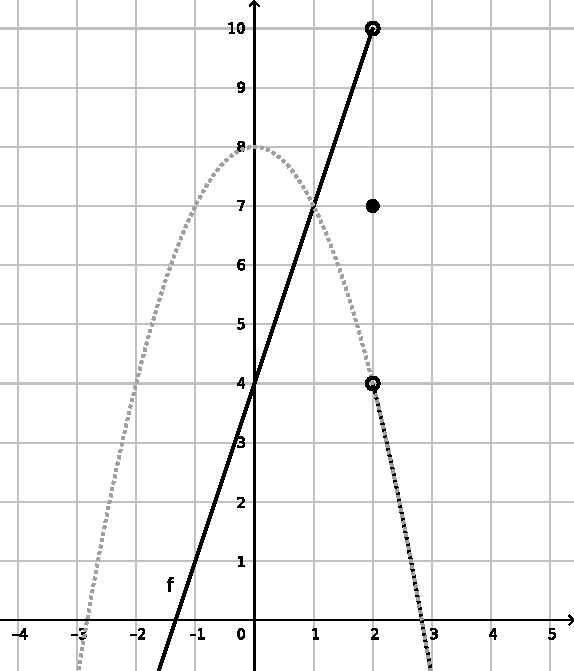
\includegraphics[width=7cm,height=6cm]{./cap_funcao/figs/funcaoPartesexem1}}
   \caption{Gráfico da função $f$}
  \end{figure}
\end{exem}

\begin{exem}
\begin{equation*}
f(x) = \begin{cases}
                 -x^2 + 1, \text{ se } x < 0 \\
                 e^x, \text{ se } x \geqslant 0
                \end{cases} \ .
\end{equation*}
   \begin{figure}[H]
  \centering
  \fbox{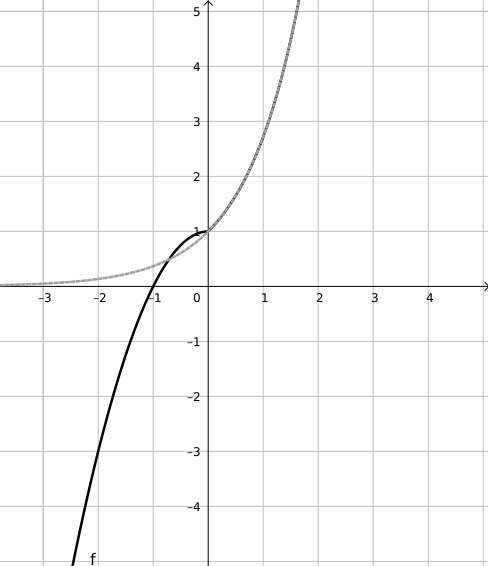
\includegraphics[height=6cm]{./cap_funcao/figs/funcaoPartesexem2}}
   \caption{Gráfico da função $f$}
  \end{figure}
\end{exem}

\begin{exem}
\begin{equation*}
f(x) = \begin{cases}
                 -x + 1, \text{ se } x \leqslant 1 \\
                 ln(x), \text{ se } x > 1
                \end{cases} \ .
\end{equation*}
\begin{figure}[H]
  \centering
  \fbox{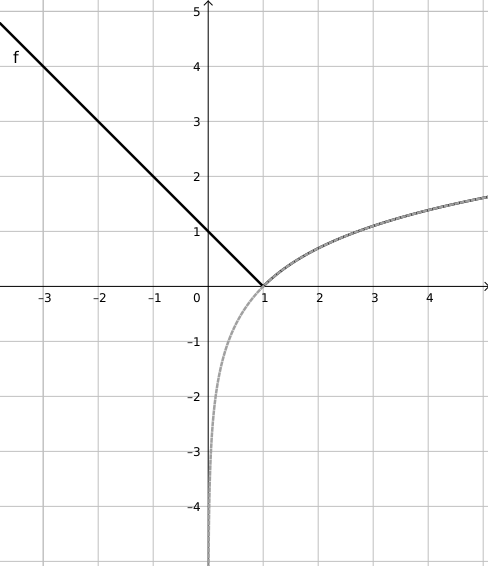
\includegraphics[height=6cm]{./cap_funcao/figs/funcaoPartesexem3}}
   \caption{Gráfico da função $f$}
  \end{figure}
\end{exem}

\begin{exem}
\begin{equation*}
f(x) = \begin{cases}
                 x^2+2x+1, \text{ se } x < 1 \\
                 5, \text{ se } x = 1 \\
                -x+5, \text{ se } x > 1
                \end{cases} \ .
\end{equation*}
\begin{figure}[H]
  \centering
  \fbox{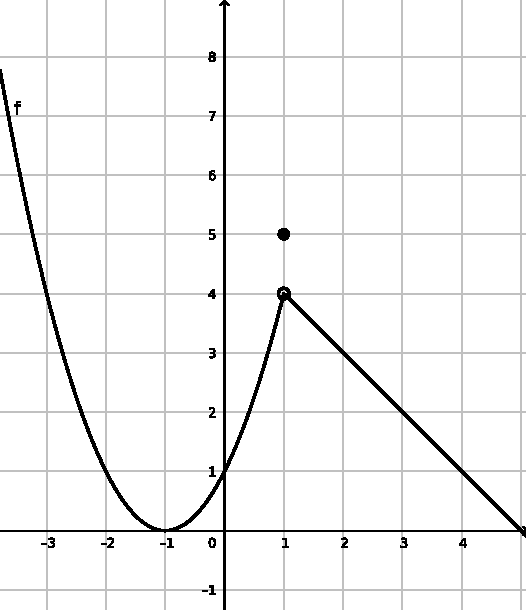
\includegraphics[height=7cm]{./cap_funcao/figs/funcaoPartesexem4}}
   \caption{Gráfico da função $f$}
  \end{figure}
\end{exem}

\section{Função modular}

  Considere a função $f: \R \rightarrow \R$, dada por $f(x)= \abs{x}$. Pela definição de módulo, temos que $f$ é uma função definida por partes, da seguinte forma:

  \[f(x)= \abs{x} = \begin{cases}
                 x, \text{ se } x \geq 0 \\
                 -x, \text{ se } x < 0.
                \end{cases}\]

O gráfico desta função é dada por

  \begin{figure}[H]
 \centering
    \fbox{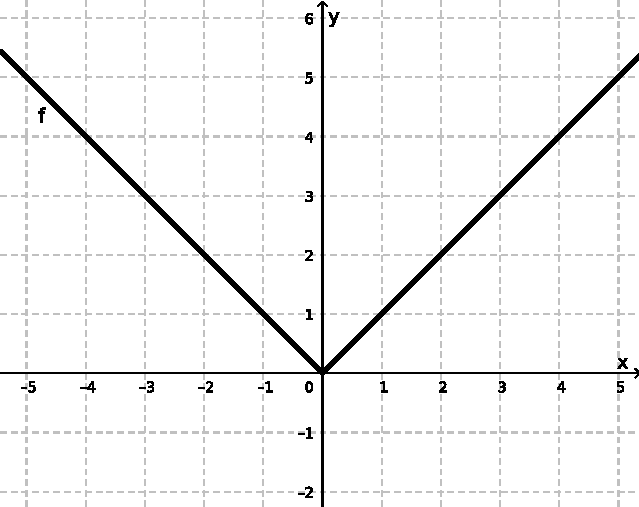
\includegraphics[width=7cm]{./cap_funcao/figs/funcaomodulo}}
    \caption{Gráfico da função módulo}
  \end{figure}

Note que, $Im(f)= [0, \infty)$ e não todo o contradomínio $\R$. Além disso, esta é uma função na qual as duas partes são lineares.
  
 \begin{exem}
 Vamos determinar os intervalos de crescimento e decrescimento, caso existam, da função $f(x)= \abs{x}$. Lembramos que esta função é definida por partes, por isso faremos a análise em cada uma destas partes.

  Caso 1: Se $x < 0$, temos que $f(x)= -x$, logo se $x_1 < x_2$,
\begin{equation*}
x_1 < x_2 \Rightarrow -x_1 > -x_2 \Rightarrow f(x_1) > f(x_2) \ ,
\end{equation*}
  por exemplo, sendo $x_1= -3$ e $x_2= -2$ temos que $x_1 < x_2$,
\begin{equation*}
f(x_1)= f(-3)= -(-3)= 3 > 2= -(-2)= f(-2)= f(x_2) \ .
\end{equation*}

  Portanto se $x < 0$ temos que $f$ é decrescente.

  Caso 2: Se $x \geq 0$, temos que $f(x)= x$, logo se $x_1 < x_2$
\begin{equation*}
x_1 < x_2 \Rightarrow  f(x_1) < f(x_2) \ ,
\end{equation*}
  por exemplo, sendo $x_1= 2$ e $x_2= 3$ temos que $x_1 < x_2$,
\begin{equation*}
f(x_1)= 2 > 3= f(x_2) \ .
\end{equation*}

  Portanto se $x \geq 0$ temos que $f$ é crescente.
 \end{exem}

\begin{exem}
  Consideramos a função $f: \R \rightarrow \R$ dada por $f(x)= \abs{x-2}$. A função $f$ pode ser escrita como:
    \begin{align*}
        f(x)& = 
        \begin{cases}
         x -2, \text{ se } x-2 \geq 0 \\
         -(x - 2), \text{ se } x-2 < 0
        \end{cases} \\
        & = 
        \begin{cases}
         x -2, \text{ se } x \geq 2 \\
         -x +2, \text{ se } x < 2.
        \end{cases}
    \end{align*}
  Com isso a função modular pode ser vista como uma função linear por partes cujo gráfico é dado por:
  \begin{center}
  \begin{tikzpicture}[scale=1]
    \tkzInit[xmin=-1, xmax=5, xstep=1, ymin=-1,ymax=3]
        %\tkzDrawXY
        \tkzAxeXY[fill=black!5]
        
        \tkzFct[thick,red,domain=2:5]{x-2}
        \tkzFct[thick,red,domain=-4:2]{-x+2}
    
        %\tkzDefPointByFct[ref=A, with=a](-1)
        %\tkzDefPoint(0,2){A}
        %\tkzDefPoint(0.5,2.25){B}
        %\tkzPointShowCoord(B)
        %\tkzDrawPoint[fill=red, size=3](A)
        %\tkzDrawPoint[fill=red, size=3](B)
        
    \end{tikzpicture}
\end{center}
\end{exem}

\begin{exem}
  Consideramos a função $f: \R \rightarrow \R$ dada por $f(x)= \abs{x+1}+2$. A função $f$ pode ser escrita como:
    \begin{align*}
        f(x)& = 
        \begin{cases}
         x +1 +2, \text{ se } x+1 \geq 0 \\
         -(x +1) +2, \text{ se } x+1 < 0
        \end{cases} \\
        & = 
        \begin{cases}
         x +3, \text{ se } x \geq 1 \\
         -x +1, \text{ se } x < -1.
        \end{cases}
    \end{align*}
  Com isso a função modular pode ser vista como uma função linear por partes cujo gráfico é dado por:
  \begin{center}
  \begin{tikzpicture}[scale=1]
    \tkzInit[xmin=-3, xmax=3, xstep=1, ymin=0,ymax=4]
        %\tkzDrawXY
        \tkzAxeXY[fill=black!5]
        
        \tkzFct[thick,red,domain=-1:3]{x+3}
        \tkzFct[thick,red,domain=-3:-1]{-x+1}
    
        %\tkzDefPointByFct[ref=A, with=a](-1)
        %\tkzDefPoint(0,2){A}
        %\tkzDefPoint(0.5,2.25){B}
        \tkzPointShowCoord((-1,2))
        %\tkzDrawPoint[fill=red, size=3](A)
        %\tkzDrawPoint[fill=red, size=3](B)
        
    \end{tikzpicture}
\end{center}
\end{exem}

\begin{exem}
  Seja $f: \R \rightarrow \R$ dada por $f(x)= \abs{x^2-3x+2}$.
  A função $f$ pode ser escrita como:
    \begin{align*}
        f(x)& = 
        \begin{cases}
         x^2-3x+2, \text{ se } x^2-3x+2 \geq 0 \\
         -(x^2-3x+2), \text{ se } x^2-3x+2 < 0.
        \end{cases}
    \end{align*}
  A maneira mais fácil de se obter o gráfico é desenhar o gráfico da função quadrática $g(x)=x^2-3x+2$ e em seguida refletir em relação ao eixo $x$ a parte do gráfico que está abaixo deste eixo $x$, como a seguir:
  \begin{center}
  \begin{tikzpicture}[scale=1]
    \tkzInit[xmin=-1, xmax=4, xstep=1, ymin=-1,ymax=4]
        %\tkzDrawXY
        \tkzAxeXY[fill=black!5]
        
        \tkzFct[thick,red,domain=-1:1]{x**2-3*x+2}
        \tkzFct[thick,red,domain=2:4]{x**2-3*x+2}
        \tkzFct[thick,red,domain=1:2]{-x**2+3*x-2}
        \tkzFct[dashed,gray,domain=1:2]{x**2-3*x+2}

        \tkzDefPoint(1.5,0.25){A}
        %\tkzDefPointByFct[ref=A, with=a](-1)
        %\tkzDefPoint(0,2){A}
        %\tkzDefPoint(0.5,2.25){B}
        \tkzPointShowCoord[xlabel=$\frac{3}{2}$]((1.5,0.25))
        %\tkzDrawPoint[fill=red, size=3](A)
        %\tkzDrawPoint[fill=red, size=3](B)
        
    \end{tikzpicture}
\end{center}
\end{exem}

\begin{exem}
  Seja $f: \R \rightarrow \R$ dada por $f(x)= \abs{2x-4}+\abs{x-1}$. Para remover os módulos desta função consideremos as funções $f_1(x)=\abs{2x-4}$ e $f_2(x)=\abs{x-1}$. Assim,
    \begin{align*}
        f_1(x)& = 
        \begin{cases}
         2x-4, \text{ se } 2x-4 \geq 0 \\
         -(2x-4), \text{ se } 2x-4 < 0.
        \end{cases}= 
        \begin{cases}
         2x-4, \text{ se } x \geq 2 \\
         -2x+4, \text{ se } x < 2,
        \end{cases} \\
        f_2(x)& = 
        \begin{cases}
         x-1, \text{ se } x-1 \geq 0 \\
         -(x-1), \text{ se } x-1 < 0.
        \end{cases}= 
        \begin{cases}
         x-1, \text{ se } x \geq 1 \\
         x-1, \text{ se } x < 1.
        \end{cases} \\
    \end{align*}

    Somando $f_1$ com $f_2$ conforme a tabela obtemos:   
    \begin{center}
    \begin{tabular}{cccc}
        %\toprule
        & $x<1$ & $1\leq x <2$  & $x \geq 2$  \\ \midrule
        $f_1(x)=|2x-4|$ & $-2x+4$ & $-2x+4$ & $2x-4$ \\ \midrule
        $f_2(x)=\abs{x-1}$ & $-x+1$ & $x-1$ & $x-1$\\ \midrule
        $f(x)=\abs{2x-4}+\abs{x-1}$ & $-3x+5$ & $-x+3$ & $3x-5$ \\
        %\bottomrule
    \end{tabular}
    \end{center}

    Ou seja, temos que
    \begin{align*}
        f(x)& = 
        \begin{cases}
         -3x+5, \text{ se } x < 1 \\
         -x+3, \text{ se } 1\leq x<2 \\
         3x-5, \text{ se } x\geq 2.
        \end{cases}
    \end{align*}
    
    Assim, o gráfico de $f$ é dado a seguir:  
  \begin{center}
  \begin{tikzpicture}[scale=1]
    \tkzInit[xmin=0, xmax=4, xstep=1, ymin=0,ymax=5]
        %\tkzDrawXY
        \tkzAxeXY[fill=black!5]
        
        \tkzFct[thick,red,domain=-1:1]{-3*x+5}
        \tkzFct[thick,red,domain=1:2]{-x+3}
        \tkzFct[thick,red,domain=2:4]{3*x-5}

        %\tkzDefPoint(1.5,0.25){A}
        %\tkzDefPointByFct[ref=A, with=a](-1)
        %\tkzDefPoint(0,2){A}
        %\tkzDefPoint(0.5,2.25){B}
        %\tkzPointShowCoord[xlabel=$\frac{3}{2}$]((1.5,0.25))
        %\tkzDrawPoint[fill=red, size=3](A)
        %\tkzDrawPoint[fill=red, size=3](B)
        
    \end{tikzpicture}
\end{center}
\end{exem}

\begin{secExercicios}
    \begin{exer}
        Dadas as funções $f:\R\to\R$ definidas a seguir, construa seus gráficos e determine sua imagem:
        \begin{enumerate}[a)]
            \item $f(x) = 
            \left\{\begin{array}{cl}
             -x-1 & \text{ se } x \leq -2 \\
             1 & \text{ se } -2< x \leq 0 \\
             x+1 & \text{ se } x>0
            \end{array}\right.$

            \item $f(x) = 
            \left\{\begin{array}{cl}
             x+3, \text{ se } x <-1 \\
             2, \text{ se } -1 \leq x \leq 1 \\
             -x, \text{ se } x>1
            \end{array}\right.$
            
            \item $f(x) = 
            \left\{\begin{array}{cl}
             -3, \text{ se } x < -2 \\
             -x-2, \text{ se } -2\leq x\leq 0 \\
             x^2, \text{ se } x>0
            \end{array}\right.$
            
            \item $f(x) = 
            \left\{\begin{array}{cl}
             -\abs{x}, \text{ se } x < -3 \\
             -2, \text{ se } -3\leq x\leq 0 \\
             x-2, \text{ se } x>0
            \end{array}\right.$

            \item $f(x) = 
            \left\{\begin{array}{cl}
             x^2-2x-8, \text{ se } x \leq 2 \text{ ou } x\geq 4 \\
             -x^2+2x+8, \text{ se } -3< x < 4
            \end{array}\right.$
        \end{enumerate}
    \end{exer}

    \begin{exer}
        Determine o gráfico e a imagem de cada uma das funções $f:\R\to\R$ a seguir:
        \begin{enumerate}[a)]
            \item $f(x)=\abs{2x+5}$
            \item $f(x)=\abs{-3x+\frac{5}{2}}$
            \item $f(x)=\abs{-x^2-x+6}$
            \item $f(x)=\abs{2x+6}-4$
            \item $f(x)=\abs{x^2-2x-2}+5$
            \item $f(x)=\abs{x}+x$
            \item $f(x)=\abs{3x-6}+x-1$
            \item $f(x)=\abs{2x^2+3x-2}+3x+2$
            \item $f(x)=\abs{4x+4}-\abs{3x-4}$
            \item $f(x)=\abs{\abs{3x+2}-3}$
            \item $f(x)=\abs{\abs{x^2-4}-6}$
        \end{enumerate}
    \end{exer}

    \begin{exer}
        Esboce o gráfico da função $f:[-1,1]\to\R$ dada por $f(x)=x+\dfrac{\abs{x}}{x}$.
    \end{exer}

    \begin{exer}
        Determine o maior domínio da função real $f$ definida por $f(x)=\dfrac{\sqrt{\abs{x}}}{x}$.
    \end{exer}

    \begin{exer}
        (UERJ) O volume de água em um tanque varia com o tempo de acordo com a seguinte equação:
        $$
        V= 10-\abs{4-2t}-\abs{2t-6}, \text{ com } t\geq 0.
        $$
        Nela, $V$ é o volume medido em $m^3$ após $t$ horas, contadas a partir de 8h da uma manhã. Determine os horários inicial e final dessa manhã em que o volume permanece constante.
    \end{exer}
    
\end{secExercicios}
%%Este trabalho está licenciado sob a Licença Creative Commons Atribuição-CompartilhaIgual 4.0 Internacional. Para ver uma cópia desta licença, visite https://creativecommons.org/licenses/by-sa/4.0/ ou envie uma carta para Creative Commons, PO Box 1866, Mountain View, CA 94042, USA.

\markboth{\sffamily\normalsize\bfseries Respostas dos Exercícios}{\sffamily\normalsize\bfseries Respostas dos Exercícios} % Set the page headers to display a Bibliography chapter name
\addcontentsline{toc}{chapter}{\textcolor{ocre}{Respostas dos Exercícios}}
\chapter*{Respostas dos Exercícios}
%\addcontentsline{toc}{Part}{Respostas dos Exercícios}
%\fancyhead[RE]{Introdução à Matemática Superior}
%\fancyhead[LO]{RESPOSTAS DOS EXERCÍCIOS}
%\fancyhead[LE,RO]{\thepage}

Devido a construção deste material, muitas respostas ainda não foram incluídas, podem conter imprecisões e erros.

\setlength{\columnseprule}{1pt}

\begin{multicols}{2}
\shipoutAnswer
\end{multicols}

\setlength{\columnseprule}{0pt}


%\setcounter{chapter}{12} 
\chapter{Função potência e polinomial}


\section{Paridade de uma função}

 \begin{obs}
  Dada um função $f: \R \rightarrow \R$.

\begin{itemize}
    \item   Dizemos que $f$ é uma \textbf{função par} se, para todo $x \in \R$,
\begin{equation*}
f(-x)= f(x) \ .
\end{equation*}
  \item Dizemos que $f$ é uma \textbf{função ímpar} se, para todo $x \in \R$,
\begin{equation*}
f(-x)= - f(x) \ .
\end{equation*}
\end{itemize}
\end{obs}


 \begin{exem}
  \begin{enumerate}[a)]
   \item A função $f(x)= x$ é uma função ímpar;
\begin{equation*}
f(-x)= -x= -f(x) 
\end{equation*}
   \item A função $f(x)= x^2$ é uma função par;
\begin{equation*}
f(-x)= (-x)^2= x^2 = f(x) 
\end{equation*}
   \item A função $f(x)= x^3$ é uma função ímpar.
\begin{equation*}
f(-x)= (-x)^3= -x^3= -f(x)
\end{equation*}

\item Note que uma função pode não ser par nem ímpar. A função $f(x)=x+1$ não é par nem ímpar pois para $x=1$ temos que $f(1)=2$ e $f(-1)=0$.
  \end{enumerate}
 \end{exem}

 \begin{exem}
  Vamos analisar a paridade de função modular $f(x)= \abs{x}$.
    Veja que $f(-x)=\abs{-x}=\abs{x}=f(x)$. Portanto $f$ é uma função par.
 \end{exem}

 \section{Função potência}

\begin{obs}
Uma \textbf{função potência} é uma função real $f:A\to\R$ da forma
\begin{equation*}
    f(x)=x^n,
\end{equation*}
onde $n$ é um valor constante.
\end{obs}

Devemos analisar a função de acordo com a escolha do valor de $n$.

\subsection{Caso $n$ natural ímpar}

Vejamos os gráficos para os casos $n=1, 3$ e $5$:
\begin{center}
  \begin{tikzpicture}[scale=0.7]
    \tkzInit[xmin=-3, xmax=3, xstep=1, ymin=-3,ymax=3]
        %\tkzDrawXY
        \tkzAxeXY
        %\tkzGrid
        %\tkzLabelX[text=blue,below = 3pt,]
        
        \tkzFct[thick,red]{x}
        \tkzText[below right, black](2,2){$y=x$}
        %\tkzFct[thick,red]{x**3}
        %\tkzFct[thick,red,domain=-1.5:1.5]{x**5}

        %\tkzDefPoint(1.5,0.25){A}
        %\tkzDefPointByFct[ref=A, with=a](-1)
        %\tkzDefPoint(0,2){A}
        %\tkzDefPoint(0.5,2.25){B}
        %\tkzPointShowCoord[xlabel=$\frac{3}{2}$]((1.5,0.25))
        %\tkzDrawPoint[fill=red, size=3](A)
        %\tkzDrawPoint[fill=red, size=3](B)
        
    \end{tikzpicture}
      \begin{tikzpicture}[scale=0.7]
    \tkzInit[xmin=-3, xmax=3, xstep=1, ymin=-3,ymax=3]
        %\tkzDrawXY
        \tkzAxeXY
        
        %\tkzFct[thick,red]{x}
        \tkzFct[thick,red]{x**3}
        \tkzText[below right, black](2,2){$y=x^3$}
        %\tkzFct[thick,red,domain=-1.5:1.5]{x**5}

        %\tkzDefPoint(1.5,0.25){A}
        %\tkzDefPointByFct[ref=A, with=a](-1)
        %\tkzDefPoint(0,2){A}
        %\tkzDefPoint(0.5,2.25){B}
        %\tkzPointShowCoord[xlabel=$\frac{3}{2}$]((1.5,0.25))
        %\tkzDrawPoint[fill=red, size=3](A)
        %\tkzDrawPoint[fill=red, size=3](B)
        
    \end{tikzpicture}
    \begin{tikzpicture}[scale=0.7]
    \tkzInit[xmin=-3, xmax=3, xstep=1, ymin=-3,ymax=3]
        %\tkzDrawXY
        \tkzAxeXY
        
        %\tkzFct[thick,red]{x}
        %\tkzFct[thick,red]{x**3}
        \tkzText[below right, black](2,2){$y=x^5$}
        \tkzFct[thick,red,domain=-1.5:1.5]{x**5}

        %\tkzDefPoint(1.5,0.25){A}
        %\tkzDefPointByFct[ref=A, with=a](-1)
        %\tkzDefPoint(0,2){A}
        %\tkzDefPoint(0.5,2.25){B}
        %\tkzPointShowCoord[xlabel=$\frac{3}{2}$]((1.5,0.25))
        %\tkzDrawPoint[fill=red, size=3](A)
        %\tkzDrawPoint[fill=red, size=3](B)
        
    \end{tikzpicture}
\end{center}

    Podemos notar que:
    \begin{itemize}
        \item Todos os gráficos passam pela origem;
        \item Todos os gráficos passam pelos pontos $(1,1)$ e $(-1,-1)$;
        \item São funções ímpares;
        \item A imagem delas é o conjunto dos reais $\R$.
    \end{itemize}

\subsection{Caso $n$ natural par}

Vejamos os gráficos para os casos $n=2, 4$ e $6$:
\begin{center}
  \begin{tikzpicture}[scale=0.7]
    \tkzInit[xmin=-3, xmax=3, xstep=1, ymin=-1,ymax=4]
        %\tkzDrawXY
        \tkzAxeXY
        %\tkzLabelX[text=blue,below = 3pt,]
        
        \tkzFct[thick,red]{x**2}
        \tkzText[below right, black](2,2){$y=x^2$}
        %\tkzFct[thick,red]{x**3}
        %\tkzFct[thick,red,domain=-1.5:1.5]{x**5}

        %\tkzDefPoint(1.5,0.25){A}
        %\tkzDefPointByFct[ref=A, with=a](-1)
        %\tkzDefPoint(0,2){A}
        %\tkzDefPoint(0.5,2.25){B}
        %\tkzPointShowCoord[xlabel=$\frac{3}{2}$]((1.5,0.25))
        %\tkzDrawPoint[fill=red, size=3](A)
        %\tkzDrawPoint[fill=red, size=3](B)
        
    \end{tikzpicture}
      \begin{tikzpicture}[scale=0.7]
    \tkzInit[xmin=-3, xmax=3, xstep=1, ymin=-1,ymax=4]
        %\tkzDrawXY
        \tkzAxeXY
        
        %\tkzFct[thick,red]{x}
        \tkzFct[thick,red,domain=-1.5:1.5]{x**4}
        \tkzText[below right, black](2,2){$y=x^4$}
        %\tkzFct[thick,red,domain=-1.5:1.5]{x**5}

        %\tkzDefPoint(1.5,0.25){A}
        %\tkzDefPointByFct[ref=A, with=a](-1)
        %\tkzDefPoint(0,2){A}
        %\tkzDefPoint(0.5,2.25){B}
        %\tkzPointShowCoord[xlabel=$\frac{3}{2}$]((1.5,0.25))
        %\tkzDrawPoint[fill=red, size=3](A)
        %\tkzDrawPoint[fill=red, size=3](B)
        
    \end{tikzpicture}
    \begin{tikzpicture}[scale=0.7]
    \tkzInit[xmin=-3, xmax=3, xstep=1, ymin=-1,ymax=4]
        %\tkzDrawXY
        \tkzAxeXY
        
        %\tkzFct[thick,red]{x}
        %\tkzFct[thick,red]{x**3}
        \tkzText[below right, black](2,2){$y=x^6$}
        \tkzFct[thick,red,domain=-1.5:1.5]{x**6}

        %\tkzDefPoint(1.5,0.25){A}
        %\tkzDefPointByFct[ref=A, with=a](-1)
        %\tkzDefPoint(0,2){A}
        %\tkzDefPoint(0.5,2.25){B}
        %\tkzPointShowCoord[xlabel=$\frac{3}{2}$]((1.5,0.25))
        %\tkzDrawPoint[fill=red, size=3](A)
        %\tkzDrawPoint[fill=red, size=3](B)
        
    \end{tikzpicture}
\end{center}

    Podemos notar que:
    \begin{itemize}
        \item Todos os gráficos passam pela origem;
        \item Todos os gráficos passam pelos pontos $(1,1)$ e $(-1,1)$;
        \item São funções pares;
        \item A imagem delas é o conjunto $\R_{+}=[0,\infty)$.
    \end{itemize}

    \subsection{Caso $n$ negativo ímpar}

Vejamos o gráfico para o caso $f(x)=x^{-1}=\frac{1}{x}$:
\begin{center}
  \begin{tikzpicture}[scale=0.7]
    \tkzInit[xmin=-3, xmax=3, xstep=1, ymin=-3,ymax=3]
        %\tkzDrawXY
        \tkzAxeXY
        %\tkzLabelX[text=blue,below = 3pt,]
        
        \tkzFct[thick,red,domain=0.1:3]{x**(-1)}
        \tkzFct[thick,red,domain=-3:-0.1]{x**(-1)}
        \tkzText[below right, black](2,2){$y=\frac{1}{x}$}
        %\tkzFct[thick,red]{x**3}
        %\tkzFct[thick,red,domain=-1.5:1.5]{x**5}

        %\tkzDefPoint(1.5,0.25){A}
        %\tkzDefPointByFct[ref=A, with=a](-1)
        %\tkzDefPoint(0,2){A}
        %\tkzDefPoint(0.5,2.25){B}
        %\tkzPointShowCoord[xlabel=$\frac{3}{2}$]((1.5,0.25))
        %\tkzDrawPoint[fill=red, size=3](A)
        %\tkzDrawPoint[fill=red, size=3](B)
        
    \end{tikzpicture}
\end{center}

    Podemos notar que:
    \begin{itemize}
        \item O maior domínio é $\R^{*}$;
        \item A imagem é $\R^{*}$;
        \item O gráfico passa pelos pontos $(1,1)$ e $(-1,-1)$;
        \item É uma função ímpar;
        \item Quando $x$ aumenta muito, as imagens se aproximam de zero. Se $x$ aumenta muito em valor absoluto, porém com sinal negativo, as imagens também se aproximam de zero;
        \item Quando $x$ se aproxima de zero por valores positivos, as imagens são cada vez maiores. Quando $x$ se aproxima de zero por valores negativos, as imagens são também cada vez menores.
    \end{itemize}

Pode-se verificar que as demais funções desse tipo, por exemplo, $f(x)=x^{-3}=\frac{1}{x^3}$ ou $f(x)=x^{-5}=\frac{1}{x^5}$ possuem um padrão gráfico semelhante ao da função $\frac{1}{x}$.

    

        \subsection{Caso $n$ negativo par}

Vejamos o gráfico para o caso $f(x)=x^{-2}=\frac{1}{x^2}$:
\begin{center}
  \begin{tikzpicture}[scale=0.7]
    \tkzInit[xmin=-3, xmax=3, xstep=1, ymin=-1,ymax=4]
        %\tkzDrawXY
        \tkzAxeXY
        %\tkzLabelX[text=blue,below = 3pt,]
        
        \tkzFct[thick,red,domain=0.1:3]{x**(-2)}
        \tkzFct[thick,red,domain=-3:-0.1]{x**(-2)}
        \tkzText[below right, black](2,2){$y=\frac{1}{x^2}$}
        %\tkzFct[thick,red]{x**3}
        %\tkzFct[thick,red,domain=-1.5:1.5]{x**5}

        %\tkzDefPoint(1.5,0.25){A}
        %\tkzDefPointByFct[ref=A, with=a](-1)
        %\tkzDefPoint(0,2){A}
        %\tkzDefPoint(0.5,2.25){B}
        %\tkzPointShowCoord[xlabel=$\frac{3}{2}$]((1.5,0.25))
        %\tkzDrawPoint[fill=red, size=3](A)
        %\tkzDrawPoint[fill=red, size=3](B)
        
    \end{tikzpicture}
\end{center}

    Podemos notar que:
    \begin{itemize}
        \item O maior domínio é $\R^{*}$;
        \item A imagem é $(0,\infty)$;
        \item O gráfico passa pelos pontos $(1,1)$ e $(-1,1)$;
        \item É uma função par;
        \item Quando $x$ aumenta muito, as imagens se aproximam de zero. Se $x$ aumenta muito em valor absoluto, porém com sinal negativo, as imagens também se aproximam de zero;
        \item Quando $x$ se aproxima de zero por valores positivos ou negativos, as imagens são cada vez maiores.
    \end{itemize}
    
    Pode-se verificar que as demais funções desse tipo, por exemplo, $f(x)=x^{-4}=\frac{1}{x^4}$ ou $f(x)=x^{-6}=\frac{1}{x^6}$ possuem um padrão gráfico semelhante ao da função $\frac{1}{x^2}$.


    \subsection{Caso $n$ seja da forma $\frac{1}{k}$}

    A função $f(x)=x^{1/k}=\sqrt[k]{x}$.

    Para $n=\frac{1}{2}$, esta é a função raiz quadrada $f(x)=\sqrt{x}$. O gráfico desta função é:
\begin{center}
  \begin{tikzpicture}[scale=0.7]
    \tkzInit[xmin=-1, xmax=6, xstep=1, ymin=-1,ymax=4]
        %\tkzDrawXY
        \tkzAxeXY
        %\tkzLabelX[text=blue,below = 3pt,]
        
        \tkzFct[thick,red,domain=0:6]{sqrt(x)}
        \tkzText[below right, black](2,1.5){$y=\sqrt{x}$}
        %\tkzFct[thick,red]{x**3}
        %\tkzFct[thick,red,domain=-1.5:1.5]{x**5}

        %\tkzDefPoint(1.5,0.25){A}
        %\tkzDefPointByFct[ref=A, with=a](-1)
        %\tkzDefPoint(0,2){A}
        %\tkzDefPoint(0.5,2.25){B}
        %\tkzPointShowCoord[xlabel=$\frac{3}{2}$]((1.5,0.25))
        %\tkzDrawPoint[fill=red, size=3](A)
        %\tkzDrawPoint[fill=red, size=3](B)
        
    \end{tikzpicture}
\end{center}

    Podemos notar que:
    \begin{itemize}
        \item O maior domínio é $\R_{+}$;
        \item A imagem é $\R_{+}$;
        \item O gráfico passa pelos pontos $(0,0)$ e $(1,1)$;
        \item O gráfico é a parte superior da parábola descrita pela equação $x=y^2$.
    \end{itemize}

Para $n=\frac{1}{3}$, esta é a função raiz cúbica $f(x)=\sqrt[3]{x}$. O gráfico desta função é:
\begin{center}
  \begin{tikzpicture}[scale=0.7]
    \tkzInit[xmin=-4, xmax=4, xstep=1, ymin=-3,ymax=3]
        %\tkzDrawXY
        \tkzAxeXY
        %\tkzLabelX[text=blue,below = 3pt,]
        
        \tkzFct[thick,red,domain=0:4]{x**(0.33)}
        \tkzFct[thick,red,domain=-4:0]{-abs(x)**(0.33)}
        \tkzText[below right, black](2,1.5){$y=\sqrt[3]{x}$}
        %\tkzFct[thick,red]{x**3}
        %\tkzFct[thick,red,domain=-1.5:1.5]{x**5}

        %\tkzDefPoint(1.5,0.25){A}
        %\tkzDefPointByFct[ref=A, with=a](-1)
        %\tkzDefPoint(0,2){A}
        %\tkzDefPoint(0.5,2.25){B}
        %\tkzPointShowCoord[xlabel=$\frac{3}{2}$]((1.5,0.25))
        %\tkzDrawPoint[fill=red, size=3](A)
        %\tkzDrawPoint[fill=red, size=3](B)
        
    \end{tikzpicture}
\end{center}

    Podemos notar que:
    \begin{itemize}
        \item O maior domínio é $\R$;
        \item A imagem é $\R$;
        \item O gráfico passa pelos pontos $(0,0)$, $(1,1)$ e $(-1,-1)$;
        \item O gráfico corresponde à cúbica descrita pela equação $x=y^3$.
    \end{itemize}
    
%  \textbf{Função raiz quadrada}

%  É a função $f: \R_{+} \to \R_{+}$ dada por $f(x)= \sqrt{x}$, cujo gráfico é:

%   \begin{figure}[H]
% \centering
%    \fbox{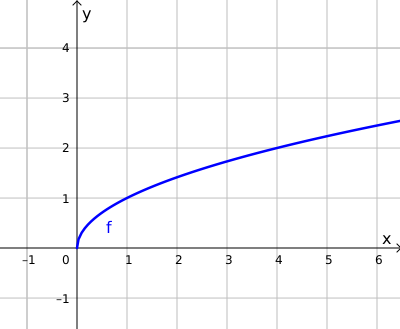
\includegraphics[width=6cm]{./cap_funcao/figs/funcaoraizquadrada}}
%    \caption{Função raiz quadrada}
%  \end{figure}

%  Note que neste caso o domínio da função são apenas os números reais positivos, já que não existe raiz quadrada de número negativo.

%  \textbf{Função raiz cúbica}

%  É a função $f: \R \to \R$ dada por $f(x)= \sqrt[3]{x}$, cujo gráfico é:

%   \begin{figure}[H]
% \centering
%    \fbox{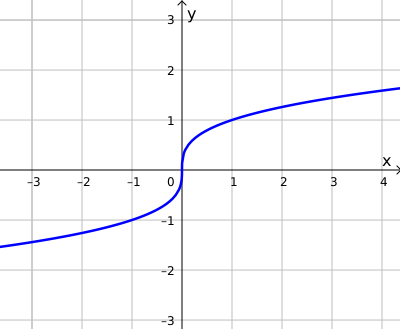
\includegraphics[width=6cm]{./cap_funcao/figs/funcaoraizcubica}}
%    \caption{Função raiz cúbica}
%  \end{figure}

%  \textbf{Função recíproca}

%  É a função $f: \R \setminus \{0\} \to \R$ dada por $f(x)= \frac{1}{x}$, cujo gráfico é:

%   \begin{figure}[H]
% \centering
%    \fbox{\includegraphics[width=6cm]{./cap_funcao/figs/funcaoreciproca}}
%    \caption{Função recíproca}
%  \end{figure}

%  Neste caso o domínio da função é o conjunto $\R \setminus \{0\}$, pois não existe divisão por $0$ (zero).

\section{Funções polinomiais de grau \texorpdfstring{$n$}{n}}

\begin{obs}
As funções $f: \R \to \R$ com a seguinte regra geral:
\begin{equation*}
f(x) = a_0 + a_1 x + a_2 x^2 + a_3 x^3 + \cdots + a_n x^n
\end{equation*}
para $\{a_0, a_1, a_2, a_3, \ldots a_n\} \in \R$ e $n \in \N$, tais que $a_n \neq 0$ são denominadas \\ \textbf{funções polinomiais de grau $n$}.
\end{obs}

Observe que as funções de 1ª e 2ª grau são exemplos de funções polinomiais. Vejamos agora um breve estudo sobre as funções polinomiais de 3º grau.

\subsection{Funções do 3º grau}
As funções do 3º grau ou funções cúbicas são funções $f: \R \rightarrow \R$ dadas por:
\begin{equation*}
f(x)= ax^3 + bx^2 + cx + d \ ,
\end{equation*}
para certos $a, b, c, d \in \R$ com $a \neq 0$. As \textbf{raízes} ou \textbf{zeros} das funções de 3º grau são os $x \in \R$ tais que $ax^3 + bx^2 + cx + d=0$. Assim as funções de 3º grau podem classificadas de acordo com suas raízes em 4 casos:
\begin{itemize}
 \item 3 raízes reais distintas. Por exemplo, o gráfico da função $f(x)= x^3-x^2-2x=x(x-2)(x+1)$ é:
 \begin{center}
    \begin{tikzpicture}[scale=1]
    \tkzInit[xmin=-4, xmax=4, xstep=1, ymin=-3,ymax=3]
        %\tkzDrawXY
        \tkzAxeXY
        %\tkzLabelX[text=blue,below = 3pt,]
        
        \tkzFct[thick,red]{x*(x-1)*(x+2)}
        %\tkzText[below right, black](2,1.5){$y=\sqrt[3]{x}$}
        %\tkzFct[thick,red]{x**3}
        %\tkzFct[thick,red,domain=-1.5:1.5]{x**5}

        %\tkzDefPoint(1.5,0.25){A}
        %\tkzDefPointByFct[ref=A, with=a](-1)
        %\tkzDefPoint(0,2){A}
        %\tkzDefPoint(0.5,2.25){B}
        %\tkzPointShowCoord[xlabel=$\frac{3}{2}$]((1.5,0.25))
        %\tkzDrawPoint[fill=red, size=3](A)
        %\tkzDrawPoint[fill=red, size=3](B)
        
    \end{tikzpicture}
\end{center}
 \item 3 raízes reais sendo duas delas iguais. Por exemplo, o gráfico da função $f(x)= 2x^3-3x^2+1=2(x+\frac{1}{2})(x-1)^2$ é:
 \begin{center}
    \begin{tikzpicture}[scale=1]
    \tkzInit[xmin=-4, xmax=4, xstep=1, ymin=-3,ymax=3]
        %\tkzDrawXY
        \tkzAxeXY
        %\tkzLabelX[text=blue,below = 3pt,]
        
        \tkzFct[thick,red]{2*x**3-3*x**2+1}
        %\tkzText[below right, black](2,1.5){$y=\sqrt[3]{x}$}
        %\tkzFct[thick,red]{x**3}
        %\tkzFct[thick,red,domain=-1.5:1.5]{x**5}

        %\tkzDefPoint(1.5,0.25){A}
        %\tkzDefPointByFct[ref=A, with=a](-1)
        %\tkzDefPoint(0,2){A}
        %\tkzDefPoint(0.5,2.25){B}
        %\tkzPointShowCoord[xlabel=$\frac{3}{2}$]((1.5,0.25))
        %\tkzDrawPoint[fill=red, size=3](A)
        %\tkzDrawPoint[fill=red, size=3](B)
        
    \end{tikzpicture}
\end{center}
 \item 3 raízes reais iguais. Por exemplo, o gráfico da função $f(x)= -x^3+6x^2-12x+8=-(x-2)^3$ é:
 \begin{center}
    \begin{tikzpicture}[scale=1]
    \tkzInit[xmin=-4, xmax=4, xstep=1, ymin=-3,ymax=3]
        %\tkzDrawXY
        \tkzAxeXY
        %\tkzLabelX[text=blue,below = 3pt,]
        
        \tkzFct[thick,red]{-(x-2)**3}
        %\tkzText[below right, black](2,1.5){$y=\sqrt[3]{x}$}
        %\tkzFct[thick,red]{x**3}
        %\tkzFct[thick,red,domain=-1.5:1.5]{x**5}

        %\tkzDefPoint(1.5,0.25){A}
        %\tkzDefPointByFct[ref=A, with=a](-1)
        %\tkzDefPoint(0,2){A}
        %\tkzDefPoint(0.5,2.25){B}
        %\tkzPointShowCoord[xlabel=$\frac{3}{2}$]((1.5,0.25))
        %\tkzDrawPoint[fill=red, size=3](A)
        %\tkzDrawPoint[fill=red, size=3](B)
        
    \end{tikzpicture}
\end{center}
 \item 1 raiz real (e duas raízes complexas). Por exemplo, o gráfico da função $f(x)= 2x^3-3x^2+2$ é:
 \begin{center}
    \begin{tikzpicture}[scale=1]
    \tkzInit[xmin=-4, xmax=4, xstep=1, ymin=-3,ymax=3]
        %\tkzDrawXY
        \tkzAxeXY
        %\tkzLabelX[text=blue,below = 3pt,]
        
        \tkzFct[thick,red]{2*x**3-3*x**2+2}
        %\tkzText[below right, black](2,1.5){$y=\sqrt[3]{x}$}
        %\tkzFct[thick,red]{x**3}
        %\tkzFct[thick,red,domain=-1.5:1.5]{x**5}

        %\tkzDefPoint(1.5,0.25){A}
        %\tkzDefPointByFct[ref=A, with=a](-1)
        %\tkzDefPoint(0,2){A}
        %\tkzDefPoint(0.5,2.25){B}
        %\tkzPointShowCoord[xlabel=$\frac{3}{2}$]((1.5,0.25))
        %\tkzDrawPoint[fill=red, size=3](A)
        %\tkzDrawPoint[fill=red, size=3](B)
        
    \end{tikzpicture}
\end{center}
\end{itemize}

% Estes casos estão representados nos gráficos abaixo, onde consideramos sempre $a> 0$, o caso $a< 0$ é análogo.




%   \begin{figure}[H]
%   \fbox{\subfigure[$a < 0$]{\includegraphics[width=7cm,height=5cm]{./cap_funcao/figs/g1}}}
%   \fbox{\subfigure[$a < 0$]{\includegraphics[width=7cm,height=5cm]{./cap_funcao/figs/g2}}}
%   \end{figure}

%  \begin{figure}[H]
%   \fbox{\subfigure[$a < 0$]{\includegraphics[width=7cm,height=5cm]{./cap_funcao/figs/g3}}}
%   \fbox{\subfigure[$a < 0$]{\includegraphics[width=7cm,height=5cm]{./cap_funcao/figs/g4}}}
%   \caption{Gráficos de funções do 3º grau}
%  \end{figure}


  

%   \textbf{Função floor}

%   É a função $f: \R \to \R$ dada por $f(x)= \lfloor {x} \rfloor$, cujo gráfico é:

%    \begin{figure}[H]
%  \centering
%     \fbox{\includegraphics[width=6cm]{./cap_funcao/figs/funcaofloor}}
%     \caption{Função floor}
%   \end{figure}

%   Esta função aplicada em um número $x$ tem como imagem a parte inteira do número $x$.

%   \textbf{Função ceil}

%   É a função $f: \R \to \R$ dada por $f(x)= \lceil {x} \rceil$, cujo gráfico é:

%    \begin{figure}[H]
%  \centering
%     \fbox{\includegraphics[width=6cm]{./cap_funcao/figs/funcaoceil}}
%     \caption{Função ceil}
%   \end{figure}

%   Esta função aplicada em um número $x$ tem como imagem o menor inteiro maior ou igual a $x$.

\begin{secExercicios}

    \begin{exer}
        Esboce os gráficos das funções a seguir, determinando seu domínio, imagem e verificando se é função par ou ímpar:
        \begin{enumerate}[a)]
            \item $f(x)=-x^3$
            \item $f(x)=x^4$
            \item $f(x)=x^{-3}$
            \item $f(x)=x^{\frac{1}{5}}$
            \item $f(x)=\sqrt[4]{x}$
            \item $f(x)=x^{-4}$
        \end{enumerate}
    \end{exer}

    \begin{exer}
        Determine se a função é par, ímpar ou nenhum dos dois:
        \begin{enumerate}[a)]
            \item $f(x)=x^5+x$
            \item $f(x)=1-x^4$
            \item $f(x)=2x-x^2$
        \end{enumerate}
    \end{exer}

    \begin{exer}
        Determine o(s) ponto(s) de interseção entre os gráficos das funções $f(x)=x$ e $g(x)=\frac{1}{x}$.
    \end{exer}
    
    \begin{exer}
        Determine a equação da reta que passa pelos pontos de interseção dos gráficos das funções $f(x)=\frac{1}{x}$ e $g(x)=\sqrt[3]{x}$.
    \end{exer}

    \begin{exer}
        Encontre a expressão para uma função cúbica $f$ tal que $f(1)=6$ e $f(-1)=f(0)=f(2)=0$.
    \end{exer}

    \begin{exer}
        (UNICAMP-2020) Seja a função polinomial do terceiro grau $f(x) = x^3 - x^2 - 2x + 1$, definida para todo número real $x$. A figura abaixo exibe o gráfico de $y=f(x)$, no plano cartesiano, em que os pontos $A$, $B$ e $C$ têm a mesma ordenada. Determine a distância entre os pontos $A$ e $C$.
         \begin{center}
    \begin{tikzpicture}[scale=0.7]
    \tkzInit[xmin=-4, xmax=4, xstep=1, ymin=-3,ymax=3]
        \tkzDrawXY[noticks]
        %\tkzAxeXY
        %\tkzLabelX[text=blue,below = 3pt,]
        
        \tkzFct[thick]{x**3 - x**2 - 2*x + 1}
        %\tkzText[below right, black](2,1.5){$y=\sqrt[3]{x}$}
        %\tkzFct[thick,red]{x**3}
        %\tkzFct[thick,red,domain=-1.5:1.5]{x**5}

        %\tkzDefPoint(1.5,0.25){A}
        %\tkzDefPointByFct[ref=A, with=a](-1)
        %\tkzDefPoint(0,2){A}
        \tkzDefPoint[label= right:$A$](-1,1){A}
        \tkzDefPoint[label= right:$B$](0,1){B}
        \tkzDefPoint[label= right:$C$](2,1){C}
        %\tkzDrawSegment(A,B)
        %\tkzDrawSegment[line width=1pt](A,C)
        \tkzPointShowCoord[noxdraw](A)
        \tkzPointShowCoord[noxdraw](C)
        \tkzDrawPoint[fill=black, size=3](A)
        \tkzDrawPoint[fill=black, size=3](B)
        \tkzDrawPoint[fill=black, size=3](C)
        
        
    \end{tikzpicture}
\end{center}
    \end{exer}
    
\end{secExercicios}
%\setcounter{chapter}{13} 
\chapter{Transformação de funções}

Podemos fazer várias mudanças nas funções de forma que seus com gráficos mudem de maneira previsível. É possível movê-los para cima e para baixo ou para os lados. Também podemos fazer espelhamentos no eixo horizontal e vertical. Por último, é possível esticar ou encolher os gráficos.

A seguir, vamos falar sobre as diferentes maneiras de alterar os gráficos das funções.

 \section{Translação vertical}

 Vejamos o seguinte exemplo:

 \begin{exem}
  Considere a função $f(x): \R \to \R$, dada por $f(x)= x^2$. Defina as seguintes funções $g,h: \R \to \R$ dadas por 
  \begin{align*}
        g(x) &= f(x) + 2= x^2 + 2,\\
        h(x) &= f(x) - 2= x^2 - 2.
  \end{align*}
  
    Observe na seguinte figura como estas transformações alteram o gráfico da função $f$:
    
    \begin{center}
  \begin{tikzpicture}[scale=0.7]
    \tkzInit[xmin=-4, xmax=4, ymin=-3,ymax=5]
        %\tkzDrawXY
        \tkzAxeXY[fill=black!5]
        %\tkzLabelX[text=blue,below = 3pt,]
        
        \tkzFct[thick,red]{x**2}
        \tkzText[above left, red](1.4,1){$f(x)$}

        \tkzFct[thick,blue]{x**2+2}
        \tkzText[above left, blue](1.4,3){$g(x)$}

        \tkzFct[thick,blue]{x**2-2}
        \tkzText[below right, blue](0.8,-1){$h(x)$}
        
        %\tkzFct[thick,red]{x**3}
        %\tkzFct[thick,red,domain=-1.5:1.5]{x**5}

        %\tkzDefPoint(1.5,0.25){A}
        %\tkzDefPointByFct[ref=A, with=a](-1)
        %\tkzDefPoint(0,2){A}
        %\tkzDefPoint(0.5,2.25){B}
        %\tkzPointShowCoord[xlabel=$\frac{3}{2}$]((1.5,0.25))
        %\tkzDrawPoint[fill=red, size=3](A)
        %\tkzDrawPoint[fill=red, size=3](B)
        
    \end{tikzpicture}
\end{center}

    Note a função $g$ carregou o gráfico da $f$ duas unidades ``para cima'' no eixo $y$, já a função $h$ carregou o gráfico da $f$ duas unidades ``para baixo'' no eixo $y$.

%  \begin{figure}[H]
%    \fbox{\subfigure[Gráficos das funções $f$ e $g$]{\includegraphics[width=7cm,height=6cm]{./cap_funcao/figs/translacaomais2}}}
%    \fbox{\subfigure[Gráficos das funções $f$ e $h$]{\includegraphics[width=7cm,height=6cm]{./cap_funcao/figs/translacaomenos2}}}
% \caption{Translação no eixo $y$}
%   \end{figure}
 \end{exem}

\begin{obs}
Suponha que $c>0$.
\begin{itemize}
    \item Para o obter o gráfico de $y=f(x)+c$, desloque o gráfico de $f(x)$ em $c$ unidades para cima;
    \item Para obter o gráfico de $y=f(x)-c$, desloque o gráfico de $f(x)$ em $c$ unidades para baixo.
\end{itemize}
\end{obs}


 %Dados $A, B \subset \R$ e uma função $f(x): A \to B$, definimos a função translação de $f$ no eixo $y$, pela função $g(x): A \to B$, dada por \destaque{g(x)= f(x) + c}, onde $c \in \R$ é uma constante.

 \section{Translação horizontal}

  Considere o seguinte exemplo:

 \begin{exem}
  Seja $f(x): \R \to \R$, dada por $f(x)= x^2$. Defina as seguintes funções $g,h: \R \to \R$ dadas por 
  \begin{align*}
        g(x) &= f(x+2)= (x+2)^2,\\
        h(x) &= f(x-2)= (x-2)^2.
  \end{align*}
  
    Observe na seguinte figura como estas transformações alteram o gráfico da função $f$:

    \begin{center}
  \begin{tikzpicture}[scale=0.7]
    \tkzInit[xmin=-4, xmax=4, ymin=-3,ymax=5]
        %\tkzDrawXY
        \tkzAxeXY[fill=black!5]
        %\tkzLabelX[text=blue,below = 3pt,]
        
        \tkzFct[thick,red]{x**2}
        \tkzText[above right, red](1.6,2){$f(x)$}

        \tkzFct[thick,blue]{(x+2)**2}
        \tkzText[above right, blue](-3,1){$g(x)$}

        \tkzFct[thick,blue]{(x-2)**2}
        \tkzText[above right, blue](3.4,1){$h(x)$}
        
        %\tkzFct[thick,red]{x**3}
        %\tkzFct[thick,red,domain=-1.5:1.5]{x**5}

        %\tkzDefPoint(1.5,0.25){A}
        %\tkzDefPointByFct[ref=A, with=a](-1)
        %\tkzDefPoint(0,2){A}
        %\tkzDefPoint(0.5,2.25){B}
        %\tkzPointShowCoord[xlabel=$\frac{3}{2}$]((1.5,0.25))
        %\tkzDrawPoint[fill=red, size=3](A)
        %\tkzDrawPoint[fill=red, size=3](B)
        
    \end{tikzpicture}
\end{center}

    Note a função $g$ carregou o gráfico da $f$ duas unidades ``para à esquerda'' no eixo $x$, já a função $h$ carregou o gráfico da $f$ duas unidades ``para à direita'' no eixo $x$.

%  \begin{figure}[H]
%    \fbox{\subfigure[Gráficos das funções $f$ e $g$]{\includegraphics[width=7cm,height=6cm]{./cap_funcao/figs/translacaomais2}}}
%    \fbox{\subfigure[Gráficos das funções $f$ e $h$]{\includegraphics[width=7cm,height=6cm]{./cap_funcao/figs/translacaomenos2}}}
% \caption{Translação no eixo $y$}
%   \end{figure}
 \end{exem}

\begin{obs}
Suponha que $c>0$.
\begin{itemize}
    \item Para o obter o gráfico de $y=f(x+c)$, desloque o gráfico de $f(x)$ em $c$ unidades para a esquerda;
    \item Para obter o gráfico de $y=f(x-c)$, desloque o gráfico de $f(x)$ em $c$ unidades para a direita.
\end{itemize}
\end{obs}

  % Dados $A, B \subset \R$ e uma função $f(x): A \to B$, definimos a função translação de $f$ no eixo $x$, pela função $g(x): A \to B$, dada por \destaque{g(x)= f(x + c)}, onde $c \in \R$ é uma constante.

%  \begin{exem}
%   Considere a função $f(x): \R \to \R$, dada por $f(x)= x^2$. Defina as seguintes funções $g: \R \to \R$ dada por $g(x)= f(x + 2)= (x+2)^2$, e $h: \R \to \R$ dada por $h(x)= f(x-2)= (x-2)^2$, observe na seguinte figura como estas translações alteram o gráfico da função $f$, 

%  \begin{figure}[H]
%    \fbox{\subfigure[Gráficos das funções $f$ e $g$]{\includegraphics[width=7cm,height=6cm]{./cap_funcao/figs/translacaoXmais2}}}
%    \fbox{\subfigure[Gráficos das funções $f$ e $h$]{\includegraphics[width=7cm,height=6cm]{./cap_funcao/figs/translacaoXmenos2}}}
% \caption{Translação no eixo $x$}
%   \end{figure}

%  \end{exem}

 \section{Reflexão do gráfico das funções}

% Dados $A, B \subset \R$ e uma função $f(x): A \to B$, definimos a função reflexão de $f$ no eixo $x$, pela função $g(x): A \to B$, dada por \destaque{g(x)= -f(x)}.

Considere o seguinte exemplo:

 \begin{exem}
  Seja $f(x): \R \to \R$, dada por $f(x)= x^2-x$. Defina a função $g: \R \to \R$ dada por
  \begin{equation*}
      g(x)=-f(x)= -x^2+x.
  \end{equation*}
  
  Note que $g$ é uma a reflexão da função $f$ em torno do eixo $x$, como pode ser visto pela figura:

    \begin{center}
  \begin{tikzpicture}[scale=0.7]
    \tkzInit[xmin=-3, xmax=3, ymin=-3,ymax=3]
        %\tkzDrawXY
        \tkzAxeXY[fill=black!5]
        %\tkzLabelX[text=blue,below = 3pt,]
        
        \tkzFct[thick,red]{x**2-x}
        \tkzText[above right, red](2,1){$f(x)$}

        \tkzFct[thick,blue]{-x**2+x}
        \tkzText[above right, blue](2,-2){$g(x)$}

        %\tkzFct[thick,red]{x**3}
        %\tkzFct[thick,red,domain=-1.5:1.5]{x**5}

        %\tkzDefPoint(1.5,0.25){A}
        %\tkzDefPointByFct[ref=A, with=a](-1)
        %\tkzDefPoint(0,2){A}
        %\tkzDefPoint(0.5,2.25){B}
        %\tkzPointShowCoord[xlabel=$\frac{3}{2}$]((1.5,0.25))
        %\tkzDrawPoint[fill=red, size=3](A)
        %\tkzDrawPoint[fill=red, size=3](B)
        
    \end{tikzpicture}
\end{center}

Por outro lado, defina $h: \R \to \R$ dada por
  \begin{equation*}
      h(x)=f(-x)= x^2+x.
  \end{equation*}
  
  Note que $g$ é uma a reflexão da função $f$ em torno do eixo $y$, como pode ser visto pela figura:

    \begin{center}
  \begin{tikzpicture}[scale=0.7]
    \tkzInit[xmin=-3, xmax=3, ymin=-1,ymax=3]
        %\tkzDrawXY
        \tkzAxeXY[fill=black!5]
        %\tkzLabelX[text=blue,below = 3pt,]
        
        \tkzFct[thick,red]{x**2-x}
        \tkzText[above right, red](2,1){$f(x)$}

        \tkzFct[thick,blue]{x**2+x}
        \tkzText[above left, blue](-2,1){$g(x)$}

        %\tkzFct[thick,red]{x**3}
        %\tkzFct[thick,red,domain=-1.5:1.5]{x**5}

        %\tkzDefPoint(1.5,0.25){A}
        %\tkzDefPointByFct[ref=A, with=a](-1)
        %\tkzDefPoint(0,2){A}
        %\tkzDefPoint(0.5,2.25){B}
        %\tkzPointShowCoord[xlabel=$\frac{3}{2}$]((1.5,0.25))
        %\tkzDrawPoint[fill=red, size=3](A)
        %\tkzDrawPoint[fill=red, size=3](B)
        
    \end{tikzpicture}
\end{center}

 \end{exem}


 % Dados $A, B \subset \R$ e uma função $f(x): A \to B$, definimos a função reflexão de $f$ no eixo $y$, pela função $g(x): A \to B$, dada por \destaque{g(x)= f(-x)}.

%  \begin{exem}
%   Seja $f(x): \R \to \R$, dada por $f(x)= x^3$. Defina a função $g: \R \to \R$ dada por 
%   \begin{equation*}
%   g(x)=f(-x)= (-x)^3.
%   \end{equation*}
  
%   Note que $g$ é uma a reflexão da função $f$ em torno do eixo $y$, como pode ser visto pela figura:

%     \begin{center}
%   \begin{tikzpicture}[scale=0.7]
%     \tkzInit[xmin=-3, xmax=3, ymin=-3,ymax=3]
%         %\tkzDrawXY
%         \tkzAxeXY[fill=black!5]
%         %\tkzLabelX[text=blue,below = 3pt,]
        
%         \tkzFct[thick,red]{x**3}
%         \tkzText[above right, red](1.4,1){$f(x)$}

%         \tkzFct[thick,blue]{-x**3}
%         \tkzText[above right, blue](1.4,-2){$g(x)$}

%         %\tkzFct[thick,red]{x**3}
%         %\tkzFct[thick,red,domain=-1.5:1.5]{x**5}

%         %\tkzDefPoint(1.5,0.25){A}
%         %\tkzDefPointByFct[ref=A, with=a](-1)
%         %\tkzDefPoint(0,2){A}
%         %\tkzDefPoint(0.5,2.25){B}
%         %\tkzPointShowCoord[xlabel=$\frac{3}{2}$]((1.5,0.25))
%         %\tkzDrawPoint[fill=red, size=3](A)
%         %\tkzDrawPoint[fill=red, size=3](B)
        
%     \end{tikzpicture}
% \end{center}

%  \end{exem}

\begin{obs}
\begin{itemize}
    \item Para o obter o gráfico de $y=-f(x)$, faça uma reflexão do gráfico de $f(x)$ em em torno do eixo $x$;
    \item Para obter o gráfico de $y=f(-x)$, faça uma reflexão do gráfico de $f(x)$ em em torno do eixo $y$.
\end{itemize}
\end{obs}


\section{Expansão e contração}

\begin{obs}
Suponha que $c>1$.
\begin{itemize}
    \item Para o obter o gráfico de $y=c\cdot f(x)$, expanda o gráfico de $f(x)$ verticalmente por um fator de $c$;
    \item Para o obter o gráfico de $y=\frac{1}{c}\cdot f(x)$, contraia o gráfico de $f(x)$ verticalmente por um fator de $c$;
    \item Para o obter o gráfico de $y= f(c\cdot x)$, contraia o gráfico de $f(x)$ horizontalmente por um fator de $c$;
    \item Para o obter o gráfico de $y= f(\frac{1}{c}\cdot x)$, expanda o gráfico de $f(x)$ horizontalmente por um fator de $c$.
\end{itemize}
\end{obs}

 \begin{exem}
     Seja $f:\R \to \R$ dada por $f(x)=x^2-2x$ e tome $c=2$. Assim, temos as seguinte situações descritas nos gráficos:

         \begin{center}
  \begin{tikzpicture}[scale=0.7]
    \tkzInit[xmin=-1, xmax=5, ymin=-2.5,ymax=3]
        %\tkzDrawXY
        \tkzAxeXY[fill=black!5]
        %\tkzLabelX[text=blue,below = 3pt,]
        
        \tkzFct[thick,red]{x**2-2*x}
        \tkzText[above right, red](3,2){$f(x)$}

        \tkzFct[thick,blue]{2*x**2-4*x}
        \tkzText[above left, blue](2.5,2){$2f(x)$}

        %\tkzFct[thick,red]{x**3}
        %\tkzFct[thick,red,domain=-1.5:1.5]{x**5}

        %\tkzDefPoint(1.5,0.25){A}
        %\tkzDefPointByFct[ref=A, with=a](-1)
        %\tkzDefPoint(0,2){A}
        %\tkzDefPoint(0.5,2.25){B}
        %\tkzPointShowCoord[xlabel=$\frac{3}{2}$]((1.5,0.25))
        %\tkzDrawPoint[fill=red, size=3](A)
        %\tkzDrawPoint[fill=red, size=3](B)
        
    \end{tikzpicture}
    \hspace{1cm}
    \begin{tikzpicture}[scale=0.7]
    \tkzInit[xmin=-1, xmax=5, ymin=-2.5,ymax=3]
        %\tkzDrawXY
        \tkzAxeXY[fill=black!5]
        %\tkzLabelX[text=blue,below = 3pt,]
        
        \tkzFct[thick,red]{x**2-2*x}
        \tkzText[above left, red](2.5,2){$f(x)$}

        \tkzFct[thick,blue]{0.5*x**2-x}
        \tkzText[below right, blue](3,1.4){$\frac{1}{2}f(x)$}

        %\tkzFct[thick,red]{x**3}
        %\tkzFct[thick,red,domain=-1.5:1.5]{x**5}

        %\tkzDefPoint(1.5,0.25){A}
        %\tkzDefPointByFct[ref=A, with=a](-1)
        %\tkzDefPoint(0,2){A}
        %\tkzDefPoint(0.5,2.25){B}
        %\tkzPointShowCoord[xlabel=$\frac{3}{2}$]((1.5,0.25))
        %\tkzDrawPoint[fill=red, size=3](A)
        %\tkzDrawPoint[fill=red, size=3](B)
        
    \end{tikzpicture}

    \begin{tikzpicture}[scale=0.7]
    \tkzInit[xmin=-1.5, xmax=5, ymin=-1,ymax=3]
        %\tkzDrawXY
        \tkzAxeXY[fill=black!5]
        %\tkzLabelX[text=blue,below = 3pt,]
        
        \tkzFct[thick,red]{x**2-2*x}
        \tkzText[above right, red](3,2){$f(x)$}

        \tkzFct[thick,blue,]{4*x**2-4*x}
        \tkzText[below right, blue](1.2,3){$f(2x)$}

        %\tkzFct[thick,red]{x**3}
        %\tkzFct[thick,red,domain=-1.5:1.5]{x**5}

        %\tkzDefPoint(1.5,0.25){A}
        %\tkzDefPointByFct[ref=A, with=a](-1)
        %\tkzDefPoint(0,2){A}
        %\tkzDefPoint(0.5,2.25){B}
        %\tkzPointShowCoord[xlabel=$\frac{3}{2}$]((1.5,0.25))
        %\tkzDrawPoint[fill=red, size=3](A)
        %\tkzDrawPoint[fill=red, size=3](B)
        
    \end{tikzpicture}
    \hspace{1cm}
    \begin{tikzpicture}[scale=0.7]
    \tkzInit[xmin=-1.5, xmax=5, ymin=-1,ymax=3]
        %\tkzDrawXY
        \tkzAxeXY[fill=black!5]
        %\tkzLabelX[text=blue,below = 3pt,]
        
        \tkzFct[thick,red]{x**2-2*x}
        \tkzText[above right, red](3,2){$f(x)$}

        \tkzFct[thick,blue]{0.25*x**2-x}
        \tkzText[above left, blue](4.5,0){$f(\frac{1}{2}x)$}

        %\tkzFct[thick,red]{x**3}
        %\tkzFct[thick,red,domain=-1.5:1.5]{x**5}

        %\tkzDefPoint(1.5,0.25){A}
        %\tkzDefPointByFct[ref=A, with=a](-1)
        %\tkzDefPoint(0,2){A}
        %\tkzDefPoint(0.5,2.25){B}
        %\tkzPointShowCoord[xlabel=$\frac{3}{2}$]((1.5,0.25))
        %\tkzDrawPoint[fill=red, size=3](A)
        %\tkzDrawPoint[fill=red, size=3](B)
        
    \end{tikzpicture}
\end{center}
 \end{exem}
 
%  Resumindo, dados $A, B \subset \R$, uma função $f(x): A \to B$, e uma constante $c \in \R$ obtemos as seguintes funções $g: A \to B$:
%   \begin{table}[H]
%  \centering
%  \begin{tabular}{|c|c|} \hline
%  \rowcolor{gray}
%   Mudança & Função \\\hline
%   Translação no eixo $y$ & $g(x)= f(x)+ c$ \\\hline
%   Translação no eixo $y$ & $g(x)= f(x)- c$ \\\hline
%   Translação no eixo $x$ & $g(x)= f(x+ c)$ \\\hline
%   Translação no eixo $x$ & $g(x)= f(x- c)$ \\\hline
%   Reflexão no eixo $x$ & $g(x)= -f(x)$ \\\hline
%   Reflexão no eixo $y$ & $g(x)= f(-x)$ \\\hline
%  \end{tabular}
% \end{table}

%\section{Aplicação em exemplos}

Para obter o gráfico de alguma função que envolva alguma transformação, é necessário identificar a função básica que a constrói e, em seguida, aplicar sucessivas transformações até chegar na função desejada.

Para entender melhor as transformações de maneira interativa, veja o seguinte material do Geogebra:

\geogebra{https://www.geogebra.org/m/zsej8zsg}{Transformação de funções}



% \begin{exem}
%     Seja $f(x)=\frac{1}{x+5}$. Veja que seu gráfico pode ser obtido a partir da função $\frac{1}{x}$ da seguinte forma:

% \begin{center}
%     \begin{tikzpicture}[scale=0.7]
%     \tkzInit[xmin=-3, xmax=3, ymin=-3,ymax=3]
%         \tkzAxeXY[fill=black!5]
%         \tkzFct[thick,red,domain=-,-0.1]{1/x}
%         \tkzFct[thick,red,domain=0.1,3]{1/x}
%     \end{tikzpicture}
% \end{center}
% \end{exem}

\begin{secExercicios}

\begin{exer}
    Faça o gráfico de cada função, começando com o gráfico de uma das funções básicas já estudadas e então aplique as transformações apropriadas.

    \begin{enumerate}[a)]
    \begin{multicols}{2}
        \item $f(x)=x+1$
        \item $f(x)=2x$
        \item $f(x)=x^2+1$
        \item $f(x)=-x^3$
        \item $f(x)=(x+1)^2$
        \item $f(x)=\sqrt{x+3}$
        \item $f(x)=\dfrac{1}{x+1}$
        \item $f(x)=\dfrac{1}{x-4}$
        \item $f(x)=1-x^2$
        \item $f(x)=x^2-4x+3$
        \item $f(x)=(x+2)^4+3$
        \item $f(x)=1+\sqrt[3]{x-1}$
        \item $f(x)=\dfrac{2}{x+1}$
        \item $f(x)=-4+\sqrt{-x}$
        \item $f(x)=|x-2|+3$
        \item $f(x)=-(x-1)^3+2$
        \item $f(x)=\dfrac{3}{x-3}$
        \item $f(x)=|x^3+1|$
    \end{multicols}
    \end{enumerate}
\end{exer}

\begin{exer}
    Considere a função $y=f(x)$ representada no seguinte gráfico:
    \begin{center}
        \begin{tikzpicture}[scale=0.7]
        \tkzInit[xmin=-4, xmax=4, ymin=-1.5,ymax=3]
        %\tkzDrawXY
        \tkzAxeXY
        %\tkzLabelX[text=blue,below = 3pt,]

        \tkzFct[thick,red,domain=-4:-2]{2}
        \tkzFct[thick,red,domain=-2:1]{-x}
        \tkzFct[thick,red,domain=1:4]{-1}

        %\tkzFct[thick,red]{x**3}
        %\tkzFct[thick,red,domain=-1.5:1.5]{x**5}

        %\tkzDefPoint(1.5,0.25){A}
        %\tkzDefPointByFct[ref=A, with=a](-1)
        %\tkzDefPoint(0,2){A}
        %\tkzDefPoint(0.5,2.25){B}
        %\tkzPointShowCoord[xlabel=$\frac{3}{2}$]((1.5,0.25))
        %\tkzDrawPoint[fill=red, size=3](A)
        %\tkzDrawPoint[fill=red, size=3](B)
        
    \end{tikzpicture}
    \end{center}

    Com base neste gráfico, desenhe o gráfico das seguintes funções:
    \begin{enumerate}[a)]
        \item $f(x)-2$
        \item $f(1-x)$
        \item $-2\cdot f(x)$
        \item $|f(x)-1|$
    \end{enumerate}
\end{exer}
    
\end{secExercicios}
 
 %\subsection*{Respostas}

%\shipoutAnswer

% %Este trabalho está licenciado sob a Licença Creative Commons Atribuição-CompartilhaIgual 4.0 Internacional. Para ver uma cópia desta licença, visite https://creativecommons.org/licenses/by-sa/4.0/ ou envie uma carta para Creative Commons, PO Box 1866, Mountain View, CA 94042, USA.

\markboth{\sffamily\normalsize\bfseries Respostas dos Exercícios}{\sffamily\normalsize\bfseries Respostas dos Exercícios} % Set the page headers to display a Bibliography chapter name
\addcontentsline{toc}{chapter}{\textcolor{ocre}{Respostas dos Exercícios}}
\chapter*{Respostas dos Exercícios}
%\addcontentsline{toc}{Part}{Respostas dos Exercícios}
%\fancyhead[RE]{Introdução à Matemática Superior}
%\fancyhead[LO]{RESPOSTAS DOS EXERCÍCIOS}
%\fancyhead[LE,RO]{\thepage}

Devido a construção deste material, muitas respostas ainda não foram incluídas, podem conter imprecisões e erros.

\setlength{\columnseprule}{1pt}

\begin{multicols}{2}
\shipoutAnswer
\end{multicols}

\setlength{\columnseprule}{0pt}



%\setcounter{part}{4}
\part{Funções reais II}
%\setcounter{chapter}{14}
%Este trabalho está licenciado sob a Licença Creative Commons Atribuição-CompartilhaIgual 4.0 Internacional. Para ver uma cópia desta licença, visite https://creativecommons.org/licenses/by-sa/4.0/ ou envie uma carta para Creative Commons, PO Box 1866, Mountain View, CA 94042, USA.

\chapter{Função composta, injetora, sobrejetora e inversa}

\section{Função composta}

\begin{obs}
Consideremos duas funções $f: A \rightarrow B$ e $g: B \rightarrow C$, com $A, B \text{ e } C \subset \R$, tais que $Im(f) \subset B$. A função composta $g \circ f: A \rightarrow C$ é definida por:
\begin{equation*}
(g \circ f)(x)= g(f(x)). 
\end{equation*}

O seguinte diagrama ajuda a entender esta definição:

\begin{center}
    \begin{tikzpicture}[scale=0.7]
    \draw[fill=blue!30] (0,0) ellipse (0.5cm and 1cm);  
    \draw[fill=blue!30] (3,0) ellipse (0.5cm and 1cm);
    \draw[fill=blue!30] (6,0) ellipse (0.5cm and 1cm);
    \draw (0,0) node{$A$};
    \draw (3,0) node{$B$};
    \draw (6,0) node{$C$};
    \draw (1.5,0.9) node{$f$};
    \draw [->] (0.7,0.2) to [out=30,in=150] (2.3,0.2);
    \draw (4.5,0.9) node{$g$};
    \draw [->] (3.7,0.2) to [out=30,in=150] (5.3,0.2);
    \draw (3,-1.8) node{$g\circ f$};
    \draw [->] (0.7,-0.7) to [out=-30,in=-150] (5.3,-0.7);
    \end{tikzpicture}
\end{center}
\end{obs}


Em geral, $g\circ f \neq f\circ g$. Assim, devemos ter cuidado na ordem que é realizada composição.

Vejamos alguns exemplos de composições de funções $\R \to \R$.

\begin{exem}
Considerando a função linear $f(x)= -2x+4$, e a função quadrática $g(x)= x^2$. Chegamos as funções compostas 
\begin{enumerate}
\item [a)] $(f \circ g)(x)= f(g(x))= -2x^2 + 4$;
\item [b)] $(g \circ f)(x)= g(f(x))= (-2x+4)^2$.
\end{enumerate}
\end{exem}

\begin{exem}
Considere a função modular $f(x)= |x|$, e a função quadrática $g(x)= x^2-x-6$. Temos as seguintes funções compostas $\R \to \R$:
\begin{enumerate}
\item [a)] $(f \circ g)(x)= f(g(x))= |x^2-x-6|$;
\item [b)] $(g \circ f)(x)= g(f(x))= |x|^2 - |x|- 6$.
\end{enumerate}
\end{exem}

\begin{exem}
Com a função modular $f(x)= |x|$, e as funções lineares $g(x)= x+1$ e $h(x)= x-1$. Obtemos as seguintes funções compostas $\R \to \R$:
\begin{enumerate}
\item [a)] $(f \circ g)(x)= f(g(x)) \Rightarrow (f \circ g)(x)= |x+1|$;
\item [b)] $(f \circ h)(x)= f(h(x)) \Rightarrow (f \circ h)(x)= |x-1|$;
\item [c)] $(g \circ f)(x)= g(f(x)) \Rightarrow (g \circ f)(x)= |x|+1$;
\item [d)] $(h \circ f)(x)= h(f(x)) \Rightarrow (h \circ f)(x)= |x|-1$.
\end{enumerate}
Em cada um dos exemplos acima podemos observar a transformação do gráfico no plano cartesiano.
\end{exem}

O maior domínio de $g\circ f$ é o conjunto de todos os valores de $x$ no domínio de $f$ tais que $f(x)$ está no domínio de $g$. Em outras palavras, $(g\circ f)(x)$ está definida sempre que tanto $f(x)$ quanto $g(f(x))$ estiverem definidas.
Assim, 
\begin{equation*}
D(g \circ f)=\{ x\in D(f) \colon f(x) \in D(g)\}.    
\end{equation*}

\begin{exem}
    Dados $f(x)=\dfrac{x^2-4}{x-1}$ e $g(x)=\dfrac{1}{x}$ encontre o maior domínio de $g\circ f$.

    Temos de $D(f)=\R-\{1\}$ e $D(g)=\R-\{0\}$. Para $f(x)$ pertencer à $D(g)$, devemos ter que $f(x)\neq 0$, ou seja, $x\neq \pm 2$. Logo, o maior domínio de $g\circ f$ é
    \begin{equation*}
        D(g\circ f) = D(f)-{\pm 2} = \R-\{1,-4,4\}.
    \end{equation*}
\end{exem}

% \begin{exem}
% Considere as funções reais:
% \begin{eqnarray}
% f(x)= -x^2 + 8x -7
% \end{eqnarray}

% \begin{eqnarray}
% g(x)= \begin{cases}
%        g_1(x)= |x|, \text{ se } x \leqslant 9 \\
%        g_2(x)= x-3, \text{ se } x > 9
% 	  \end{cases}
% \end{eqnarray}
% Determine a função $(g \circ f)(x)= g(f(x))$.
% \begin{resol}
% Para fazer esta composição como a função $g$ é definida por partes precisamos qual é o conjunto imagem da função $f$. Note que $f$ é uma função do 2º grau com $a< 0$ logo concavidade voltada para baixo, o que nos diz que $Im(f)= (-\infty, y_v]$, por tanto basta calcular o $y_v$,
% \begin{eqnarray}
% y_v= \dfrac{- \Delta}{4a}= \dfrac{-(8^2-4.(-1).(-7))}{4.(-1)}= \dfrac{-36}{-4}= 9 \ .
% \end{eqnarray}
% Portanto, $Im(f)= (-\infty, 9]$. Assim, considerando a definição da função $g$, temos que
% \begin{eqnarray}
% (g \circ f)(x)= g(f(x))= g_1(f(x))= |-x^2 + 8x -7| \ .
% \end{eqnarray}
% \end{resol}
% \end{exem}

% \begin{exem}
% Considere as funções reais:
% \begin{eqnarray}
% f(x)= \begin{cases}
%       f_1(x)= -x^2+8x-7, \text{ se } x < 6 \\
%       f_2(x)= x-1, \text{ se } x \geqslant 6
%       \end{cases}
% \end{eqnarray}

% \begin{eqnarray}
% g(x)= \begin{cases}
%       g_1(x)= |x|, \text{ se } x < 5 \\
%       g_2(x)= 2x-5, \text{ se } 5 \leqslant x \leqslant 9 \\
%       g_3(x)= -x+22, \text{ se } x > 9
%       \end{cases}
% \end{eqnarray}
% Determine a função $(g \circ f)(x)= g(f(x))$.

%   \begin{figure}[H]
%  \centering
%     \fbox{\includegraphics[width=8cm]{./cap_funcao/figs/funcaoCompostaexem5}}
%     \caption{Gráfico da função $f$}
%   \end{figure}

% \begin{resol}
% Como a função $g$ está definida por partes, para fazer a composição precisamos entender o comportamento do conjunto imagem da função $f$. Observamos que:
% \begin{eqnarray}
% \begin{cases}
% f_1: (-\infty, 6) \to (-\infty, 9) \\
% f_2: [6, \infty) \to [5, \infty) \ .
% \end{cases}
% \end{eqnarray}
%  Com isso vemos que 
%  \begin{eqnarray}
% (g \circ f)(x)= \begin{cases}
%       g_1(f_1(x))= |-x^2+8x-7|, \text{ se } x < 2 \\
%       g_2(f_1(x))= 2*(-x^2+8x-7), \text{ se } 2 \leqslant x < 6 \\
%       g_2(f_2(x))= 2*(x-1)-5, \text{ se } 6 \leqslant x \leqslant 10 \\
%       g_3(f_2(x))= -(x-1)+22, \text{ se } x > 10
%       \end{cases}
% \end{eqnarray}
% \end{resol}
% \end{exem}

% \begin{exem}
% Considere as funções reais:
% \begin{eqnarray}
% f: [0, 2\pi] \to [-1, 1] \\
% f(x)= sen(x)
% \end{eqnarray}

% \begin{eqnarray}
% g(x)= \begin{cases}
%       g_1(x)= -2x, \text{ se } x < -1 \\
%       g_2(x)= 2|x|, \text{ se } -1 \leqslant x < 0 \\
%       g_3(x)= 4x, \text{ se } 0 \leqslant x \leqslant 1 \\
%       g_4(x)= x^2 + 3, \text{ se } x > 1
%       \end{cases}
% \end{eqnarray}
% Determine a função $(g \circ f)(x)= g(f(x))$.

% \begin{resol}
% Sabemos que $Im(f)= [-1, 1]$, logo
% \begin{eqnarray}
% g(f(x))= \begin{cases}
%       g_2(f(x))= 2|sen(x)|, \text{ se } \pi \leqslant x < 2\pi \\
%       g_3(f(x))= 4*sen(x), \text{ se }  0 \leqslant x \leqslant \pi \\
%       \end{cases}
% \end{eqnarray}
%   \begin{figure}[H]
%  \centering
%     \fbox{\includegraphics[width=8cm]{./cap_funcao/figs/funcaoCompostaexem6}}
%     \caption{Gráfico da função $(g \circ f)(x)$}
%   \end{figure}
% \end{resol}
% \end{exem}

% \begin{exem}
% As funções:
% \begin{itemize}
% \item $h_1: \R \setminus \{k*\pi \mid k \in \Z\} \to \R$ dada por $h_1(x)= \dfrac{1}{sen(x)}$;
%   \begin{figure}[H]
%  \centering
%     \fbox{\includegraphics[width=8cm]{./cap_funcao/figs/funcaoCompostaexem7h1}}
%     \caption{Gráfico da função $h_1(x)$}
%   \end{figure}
% \item $h_2: \R \setminus \{0\} \to \R$ dada por $h_2(x)= sen \left(\dfrac{1}{x} \right)$
%   \begin{figure}[H]
%  \centering
%     \fbox{\includegraphics[width=8cm]{./cap_funcao/figs/funcaoCompostaexem7h2}}
%     \caption{Gráfico da função $h_2(x)$}
%   \end{figure}
% \end{itemize}
% podem ser entendidas como composição das funções $f(x)= sen(x)$ e $g(x)= \dfrac{1}{x}$, com as devidas restrições nos conjuntos domínio. Observe que $h_1(x)= g(f(x))$ e $h_2(x)= f(g(x))$.
% \end{exem}


\section{Funções injetoras e/ou sobrejetoras}

\begin{itemize}
 \item \textbf{Injetora}

 Uma função $f: A \rightarrow B$ é injetiva, ou injetora quando:
\begin{equation*}
 x_1 \neq x_2 \in A \Rightarrow f(x_1) \neq f(x_2) \in B ,
\end{equation*}
 ou equivalentemente usando a contrapositiva:
\begin{equation*}
f(x_1) = f(x_2) \in B \Rightarrow x_1 = x_2 .
\end{equation*}

 Ou seja, $f$ é injetora quando cada elemento da $Im(f)$ recebe um único elemento de $A= Dom(f)$. Neste caso pode ocorrer de alguns elementos de $B$ não serem imagem de nenhum elemento de $A$ pela função $f$.

\begin{obs}
    Graficamente, uma função $f$ é injetora se a interseção do gráfico $f$ com qualquer reta horizontal $(y=c)$ é, no máximo, um ponto.
\end{obs}

 \item \textbf{Sobrejetora}

 Uma função $f: A \rightarrow B$ é sobrejetiva, ou sobrejetora quando para todo $y \in B$, existe pelo menos um elemento $x \in A$ tal que $f(x) = y$.
 %Equivalentemente em símbolos:
% \begin{equation*}
% \forall y \in B, \exists x \in A \text{ tal que } f(x) = y
% \end{equation*}
 Ou ainda, $f$ é sobrejetora quando o conjunto $Im(f)$ é igual ao contra-domínio $B$. Neste caso, este elemento pode não ser único.

 \item \textbf{Bijetora}

 Uma função $f: A \rightarrow B$ é bijetora, ou bijetiva quando for simultaneamente injetora e sobrejetora.
 %Neste caso, $f$ admite uma inversa que é denotada por $f^{(-1)}$.

\end{itemize}

\begin{multicols}{2}
\begin{figure}[H]
\centering
 \begin{tikzpicture}
 \node (1) at (0,0) {1};%\filldraw(1.east) circle (1pt)
 \node (2) [below of=1] {2};%\filldraw(2.east) circle (1pt)
 \node (3) [below of=2] {3};%\filldraw(3.east) circle (1pt)
 \node[fit=(1) (2) (3),ellipse,draw=red,minimum width=1cm,thick,label=below:\(A\)]{};

 \node (a) at (3,0) {a};%\filldraw($b_1$.west) circle (1pt)
 \node (b) [below of=a] {b};%\filldraw($b_2$.west) circle (1pt)
 \node (c) [below of=b] {c};%\filldraw($b_3$.west) circle (1pt)
 \node[fit=(a) (b) (c),ellipse,draw=green,minimum width=1cm,thick,label=below:\(B\)]{};

 \draw[->, shorten >=.1cm, >=stealth'] (1.east) to (c.west);
 \draw[->, shorten >=.1cm, >=stealth'] (2.east) to (b.west);
 \draw[->, shorten >=.1cm, >=stealth'] (3.east) to (a.west);
\end{tikzpicture}
\caption{Função bijetora}
\end{figure}

\begin{figure}[H]
\centering
 \begin{tikzpicture}
 \node (1) at (0,0) {1};%\filldraw(1.east) circle (1pt)
 \node (2) [below of=1] {2};%\filldraw(2.east) circle (1pt)
 \node (3) [below of=2] {3};%\filldraw(3.east) circle (1pt)
 \node[fit=(1) (2) (3),ellipse,draw=red,minimum width=1cm,thick,label=below:\(A\)]{};

 \node (a) at (3,0) {a};%\filldraw($b_1$.west) circle (1pt)
 \node (b) [below of=a] {b};%\filldraw($b_2$.west) circle (1pt)
 \node[fit=(a) (b),ellipse,draw=green,minimum width=1cm,thick,label=below:\(B\)]{};

 \draw[->, shorten >=.1cm, >=stealth'] (1.east) to (a.west);
 \draw[->, shorten >=.1cm, >=stealth'] (2.east) to (a.west);
 \draw[->, shorten >=.1cm, >=stealth'] (3.east) to (b.west);
\end{tikzpicture}
\caption{Função sobrejetora e não injetora}
\end{figure}
\end{multicols}


\begin{multicols}{2}
\begin{figure}[H]
\centering
 \begin{tikzpicture}
 \node (1) at (0,0) {1};%\filldraw(1.east) circle (1pt)
 \node (2) [below of=1] {2};%\filldraw(2.east) circle (1pt)
 \node (3) [below of=2] {3};%\filldraw(3.east) circle (1pt)
 \node[fit=(1) (2) (3),ellipse,draw=red,minimum width=1cm,thick,label=below:\(A\)]{};

 \node (a) at (3,0) {a};%\filldraw($b_1$.west) circle (1pt)
 \node (b) [below of=a] {b};%\filldraw($b_2$.west) circle (1pt)
 \node (c) [below of=b] {c};%\filldraw($b_3$.west) circle (1pt)
 \node[fit=(a) (b) (c),ellipse,draw=green,minimum width=1cm,thick,label=below:\(B\)]{};

 \draw[->, shorten >=.1cm, >=stealth'] (1.east) to (b.west);
 \draw[->, shorten >=.1cm, >=stealth'] (2.east) to (b.west);
 \draw[->, shorten >=.1cm, >=stealth'] (3.east) to (a.west);
\end{tikzpicture}
\caption{Função não sobrejetora e não injetora}
\end{figure}

\begin{figure}[H]
\centering
 \begin{tikzpicture}
 \node (1) at (0,0) {1};%\filldraw(1.east) circle (1pt)
 \node (2) [below of=1] {2};%\filldraw(2.east) circle (1pt)
 \node (3) [below of=2] {3};%\filldraw(3.east) circle (1pt)
 \node[fit=(1) (2) (3),ellipse,draw=red,minimum width=1cm,thick,label=below:\(A\)]{};

 \node (a) at (3,0) {a};%\filldraw($b_1$.west) circle (1pt)
 \node (b) [below of=a] {b};%\filldraw($b_2$.west) circle (1pt)
 \node (c) [below of=b] {c};%\filldraw($b_3$.west) circle (1pt)
 \node (d) [below of=c] {d};%\filldraw($b_3$.west) circle (1pt)
 \node[fit=(a) (b) (c) (d),ellipse,draw=green,minimum width=1cm,thick,label=below:\(B\)]{};

 \draw[->, shorten >=.1cm, >=stealth'] (1.east) to (b.west);
 \draw[->, shorten >=.1cm, >=stealth'] (2.east) to (c.west);
 \draw[->, shorten >=.1cm, >=stealth'] (3.east) to (a.west);
\end{tikzpicture}
\caption{Função não sobrejetora e injetora}
\end{figure}
\end{multicols}

% \begin{exem}

%  \begin{enumerate}
%   \item $f: \mathbb{R} \rightarrow \mathbb{R}$ tal que $f(x) = x^2$

%   Neste caso, $f$ não é sobrejetora, nem injetora.

%   \begin{proof}

%    \begin{itemize}
%     \item Sobrejetora

%     $f$ não é sobrejetora porque $x^2 \geq 0$, $\forall x \in \mathbb{R}$, logo se considerarmos $y < 0 \in \mathbb{R}$ teremos que $\nexists x \in \mathbb{R}$ tal que $f(x)= y$. Portanto $f$ não é sobrejetora.
%     \fim
%     \item Injetora

%      Note que $ \forall x \in \mathbb{R} \Rightarrow -x \in \mathbb{R}$ e que
% \begin{equation*}
% f(-x)= (-x)^2 = (-x)*(-x) = (x)*(x) = x^2 = f(x)
% \end{equation*}
%     o que mostra que $f$ não é injetora.
%    \end{itemize}
%   \end{proof}

%   \item $f: \mathbb{R_{+}} \rightarrow \mathbb{R}$ tal que $f(x) = x^2$

%   Neste caso, $f$ não é sobrejetora, mas é injetora.

%   \begin{proof}
%    \begin{itemize}
%     \item Sobrejetora

%     $f$ não é sobrejetora porque $x^2 \geq 0$, $\forall x \in \mathbb{R}$, logo se considerarmos $y < 0 \in \mathbb{R}$ teremos que $\nexists x \in \mathbb{R}$ tal que $f(x)= y$. Portanto $f$ não é sobrejetora.
%     \fim
%     \item Injetora

%     Tome $x_1=x_2 \in \mathbb{R_{+}}$ qualquer, como
% \begin{equation*}
% x_1=x_2 \Rightarrow x_1^2=x_2^2 \Rightarrow f(x_1)=f(x_2)
% \end{equation*}
%     logo $f$ é injetora.

%    \end{itemize}
%   \end{proof}

%   \item $f: \mathbb{R} \rightarrow \mathbb{R_{+}}$ tal que $f(x) = x^2$

%   Neste caso, $f$ é sobrejetora, mas não é injetora.

%   \begin{proof}
%    \begin{itemize}
%     \item Sobrejetora

%     Tome $y \in \mathbb{R_{+}}$ qualquer, como $y \geq 0$ existe $x \in \mathbb{R}$ tal que
% \begin{equation*}
% x = \sqrt{y} \Rightarrow x^2 = (\sqrt{y})^2 \Rightarrow x^2 = y \Rightarrow f(x) = y 
% \end{equation*}
%     portanto $f$ é sobrejetora.
%     \fim
%     \item Injetora

%     Note que $ \forall x \in \mathbb{R} \Rightarrow -x \in \mathbb{R}$ e que
% \begin{equation*}
% f(-x)= (-x)^2 = (-x)*(-x) = (x)*(x) = x^2 = f(x)
% \end{equation*}
%     o que mostra que $f$ não é injetora.

%    \end{itemize}
%   \end{proof}

%   \item $f: \mathbb{R_{+}} \rightarrow \mathbb{R_{+}}$ tal que $f(x) = x^2$ ou $f: \mathbb{R_{-}} \rightarrow \mathbb{R_{+}}$ tal que $f(x) = x^2$

%   Neste caso, $f$ é sobrejetora, e é injetora, portanto bijetora.

%   \begin{proof}
%    \begin{itemize}
%     \item Sobrejetora

%     Tome $y \in \mathbb{R_{+}}$ qualquer, como $y \geq 0$ existe $x \in \mathbb{R}$ tal que
% \begin{equation*}
% x = \sqrt{y} \Rightarrow x^2 = (\sqrt{y})^2 \Rightarrow x^2 = y \Rightarrow f(x) = y
% \end{equation*}
%     portanto $f$ é sobrejetora.
%     \fim
%     \item Injetora

%     Tome $x_1, x_2 \in \R_{+}$, tais que $f(x_1) = f(x_2)$ logo,
% \begin{equation*}
% f(x_1) = f(x_2) \Rightarrow x_1^2= x_2^2 \Rightarrow \sqrt{x_1^2}= \sqrt{x_2^2} \Rightarrow \abs{x_1}= \abs{x_2} \Rightarrow x_1= x_2, 
% \end{equation*}
%     pois $x_1, x_2 \geqslant 0$. Portanto $f$ é injetora.

%    \end{itemize}
%   \end{proof}

%  \end{enumerate}

% \end{exem}

\begin{exem}
    Considere a função $f:\R\to \R$ dada por $f(x)=x^2$.

    A função não é injetora pois $f(1)=1=f(-1)$. Ela também não é sobrejetora pois $Im(f)=R_+\neq \R$.
\end{exem}

\begin{exem}
    Considere agora a função $f:\R_+\to \R$ dada por $f(x)=x^2$.

    A função é injetora pois podemos ver no gráfico dela que qualquer reta horizontal intersepta no máximo é um único ponto o seu gráfico. No entanto, ela não é sobrejetora.


\end{exem}

\begin{exem}
    A função $f:\R_+\to \R_+$ dada por $f(x)=x^2$ é bijetora.
\end{exem}

\section{Função inversa}

 Considere uma função $f: A \rightarrow B$, para $A, B \subset \R$. Se existir uma função $g: B \rightarrow A$ tal que:
 \[(g \circ f)(x)= x,\ \forall x \in A \ \ \ \text {e} \ \ \
 (f \circ g)(x)= x,\ \forall x \in B\]
 dizemos que $f$ é inversível e que $g$ é a inversa de $f$. Denotamos $g= f^{-1}$.

 Ficamos com a seguinte pergunta: Quando existe $f^{-1}$? E a resposta é:


\begin{obs}
 Uma função $f: A \to B$ é inversível se, e somente se, $f$ for bijetora, ou seja, injetora e sobrejetora.
\end{obs}

O gráfico da função inversa $f^{-1}$ é simétrico ao gráfico da função $f$ em relação à reta $y = x$. Isto é importante pois permite-se analisar o comportamento dessas funções mesmo sem descrever sua expressão.

\begin{exem}
    Seja $f:\R\to\R$ dada por $y=f(x)=\frac{x}{2}$. Esta função é bijetora e, portanto, inversível. Para encontrar sua inversa, trocamos a variável $x$ por $y$ e vice-versa, e isolamos o valor de $y$ na expressão. Assim,
    \begin{align*}
        x =\frac{y}{2} \ \  \Rightarrow \ \ y =2x \Rightarrow \ \ f^{-1}(x) =2x.
    \end{align*}

    Note que seu gráfico é dado por
    \begin{center}
    \begin{tikzpicture}[scale=1]
    \tkzInit[xmin=-2, xmax=2, ymin=-2,ymax=2]
        %\tkzDrawXY
        \tkzAxeXY[fill=black!5]
        
        \tkzFct[thick,red]{0.5*x}

        \tkzFct[thick,blue]{2*x}
        \tkzFct[gray]{x}

        \draw[red, above right] (2,1) node{$f(x)$};
        \draw[blue, above right] (1,2) node{$f^{-1}(x)$};
        %\tkzDefPointByFct[ref=A, with=a](-1)
        %\tkzDefPoint(0,4){A}
        %\tkzDefPoint(2,0){B}
        %\tkzPointShowCoord(A)
        %\tkzDrawPoint[fill=red, size=3](A)
        %\tkzDrawPoint[fill=red, size=3](B)
    \end{tikzpicture}
    \end{center}
\end{exem}

\begin{exem}
    Seja $f:\R_{+}\to\R_{+}$ dada por $y=f(x)=x^2$. Como é bijetora, sua função inversa é dada por
    \begin{align*}
        x =y^2 \ \  \Rightarrow \ \ y =\sqrt{x} \Rightarrow \ \ f^{-1}(x) =\sqrt{x}.
    \end{align*}

    Seu gráfico é dado por
    \begin{center}
    \begin{tikzpicture}[scale=1]
    \tkzInit[xmin=0, xmax=3, ymin=0,ymax=3]
        %\tkzDrawXY
        \tkzAxeXY[fill=black!5]
        
        \tkzFct[thick,red]{x**2}

        \tkzFct[thick,blue]{sqrt(x)}
        \tkzFct[gray]{x}

        \draw[red, above left] (1.5,2) node{$f(x)$};
        \draw[blue, below right] (2,1.5) node{$f^{-1}(x)$};
        %\tkzDefPointByFct[ref=A, with=a](-1)
        %\tkzDefPoint(0,4){A}
        %\tkzDefPoint(2,0){B}
        %\tkzPointShowCoord(A)
        %\tkzDrawPoint[fill=red, size=3](A)
        %\tkzDrawPoint[fill=red, size=3](B)
    \end{tikzpicture}
    \end{center}
\end{exem}
% \begin{exem}
%  A função $f: \R \rightarrow \R$ dada por $f(x)= x+2$ é injetora, e sobrejetora portanto, existe uma função $g: \R \rightarrow \R$ dada por $g(x)= x-2$, tal que:
% \begin{eqnarray}
% (f \circ g)(x)&=& (x-2) + 2= x-2+2= x \\
% \Rightarrow (f \circ g)(x)&=& Id(x)
% \end{eqnarray}
% e ainda,
% \begin{eqnarray}
% (g \circ f)(x)&=& (x+2) - 2= x+2-2= x \\
% \Rightarrow (g \circ f)(x)&=& Id(x) ,
% \end{eqnarray}
% logo $g= f^{-1}$ é a função inversa de $f$.

%  \begin{figure}[H]
%  \centering
%     \fbox{\includegraphics[width=8cm]{./cap_funcao/figs/funcao_composta}}
%     \caption{Composta das funções $f$ e $g$}
%   \end{figure}

% \end{exem}

\begin{secExercicios}

\begin{exer}
    Se $f(x)=5x+3$ e $h(x)=1-2x$, calcule $f(h(1))+h(f(1))$.
\end{exer}

\begin{exer}
    Dadas as funções $f(x)=x^2+2x$ e $g(x)=-3x+1$ com domínios reais, determine:
    \begin{enumerate}[a)]
    \begin{multicols}{3}
        \item $f(g(x))$
        \item $g(f(x))$
        \item $f(f(x))$
    \end{multicols}
    \end{enumerate}
\end{exer}

\begin{exer}
    Dadas $f(x)=2x+1$ e $f(g(x))=2x+9$, determine $g(x)$.
\end{exer}

\begin{exer}
    Sejam $f(x)=\sqrt{x-1}$ e $g(x)=2x^2-5x+3$. Determine o maior domínio das funções $f\circ g$ e $g\circ f$.
\end{exer}

\begin{exer}
    Sejam $f(x)=\dfrac{x+1}{x-2}$ e $g(x)=2x+3$. Determine o maior domínio das funções $f\circ g$ e $g\circ f$.
\end{exer}

\begin{exer}
    Para cada uma das funções a seguir, diga se é injetora, sobrejetora, bijetora ou nenhum dos casos.
    \begin{enumerate}[a)]
        \item $f:(-1,1)\to \R$, com $f(x)=x^3$.
        \item $f: \R^*\to\R^*$, com $f(x)=\frac{1}{x}$.
        \item $f:\R\to\R$, com
        $f(x)= \left\{
            \begin{matrix}
                x^2, & \mbox{se } x\geq 0\\
                x, & \mbox{se } x<0.
            \end{matrix}
            \right.$

        \item $f:\R\to\R$,
       $f(x)= \left\{
            \begin{matrix}
                x-1, & \mbox{ se } x\geq 1\\
                0, & \mbox{ se } -1< x< 1\\
                x+1, & \mbox{ se } x\leq -1.
            \end{matrix}
            \right.$
    \end{enumerate}
\end{exer}

\begin{exer}
    Determine a função inversa de cada uma das funções definidas de $\R$ em $\R$:
    \begin{enumerate}[a)]
        \begin{multicols}{2}
            \item $f(x)=3x+2$
            \item $f(x)=\frac{4x+1}{3}$
            \item $f(x)=x^3+2$
            \item $f(x)=(x-1)^2+2$
            \item $f(x)=\sqrt[3]{x+2}$
            \item $f(x)=\sqrt{1-x^2}$
        \end{multicols}
    \end{enumerate}
\end{exer}

\begin{exer}
    A função $f:\R\to\R$ dada por $f(x)=x^4+1$ admite inversa? Justifique sua resposta.
\end{exer}

\begin{exer}
    Considere a função $f:[a,+\infty)\to\R_+$ dada por $f(x)=x^2-2x+1$, onde $a$ é algum valor real constante.
    \begin{enumerate}[a)]
        \item Qual é o menor valor de $a$ de modo que $f$ seja injetora?
        \item Determine sua função inversa.
    \end{enumerate}
\end{exer}

\begin{exer}
    Considere a função real $f:A\to B$ dada pela expressão
    \begin{equation*}
        f(x)=\dfrac{x+2}{x+1}.
    \end{equation*}
    \begin{enumerate}[a)]
        \item Determine $A$ e $B$ de modo que $f$ seja inversível.
        \item Calcule $f^{-1}$.
        \item Esboce os gráficos de $f$ e $f^{-1}$.
    \end{enumerate}
\end{exer}
\end{secExercicios}

%\subsection*{Respostas}
%\shipoutAnswer



% \setcounter{chapter}{15} 
%\chapter{Funções exponenciais e logarítmicas}
 \chapter{Funções exponenciais}

\begin{obs}
 A função $f: \R \rightarrow \R$ dada por
\begin{equation*}
f(x) = a^x
\end{equation*}
 com $a>0$ e $a \neq 1$ é denominada função exponencial de base $a$ definida para todo $x$ real.
\end{obs}

 Observe que:
 \begin{itemize}
 \item Sempre temos que $f(0)=1$, ou seja, o gráfico de $a^x$ deve passar pelo ponto $(0,1)$;
 \item $a^x > 0$ para todo $x\in\R$;
 \item o maior domínio é o conjunto dos números reais;
 \item a imagem da função de domínio real é o conjunto dos números estritamente positivos $\R_{+}^*$.
  \item exigimos que a constante $a$ fosse positiva para garantir que a função estivesse definida para todo $x$ real (lembre-se que, por exemplo, $\sqrt{a}= a^{\frac{1}{2}}$ não está definida para $a$ negativo);
  \item excluímos $a=1$, pois $1^x=1$ para todo $x$ real, de modo que $f(x)= 1^x$ é uma função constante.
 \end{itemize}

 \begin{exem}\label{ex:exp-2}
  Considere a função $f: \R \rightarrow \R $ dada por,
\begin{equation*}
f(x) = 2^x \ , 
\end{equation*}
  
  Vamos determinar alguns pontos do gráfico da função $f$.

  \begin{table}[H]
  \centering
  \begin{tabular}{|c|c|} \hline
  \rowcolor{gray}
  $x$ & $y=2^x$ \\ \hline
  $-2$ & $\frac{1}{4}$ \\ \hline
  $-1$ & $\frac{1}{2}$ \\ \hline
  $0$ &  $1$ \\ \hline
  $1$ &  $2$ \\ \hline
  $2$ &  $4$ \\ \hline
  \end{tabular}
  \end{table}

  Marcando estes pontos no plano cartesiano e ligando obtemos o seguinte gráfico para esta função.

    \begin{center}
    \begin{tikzpicture}[scale=1]
    \tkzInit[xmin=-2.5, xmax=2.5, ymin=0,ymax=5]
        %\tkzDrawXY
        \tkzAxeXY[fill=black!5]
        
        \tkzFct[thick,red,samples=50,domain=-2.5:2.5]{2**x}
        \tkzDrawPoint[fill=red, size=3](0,1)
        \tkzDrawPoint[fill=red, size=3](1,2)
        \tkzDrawPoint[fill=red, size=3](2,4)
        \tkzDrawPoint[fill=red, size=3](-1,0.5)
        \tkzDrawPoint[fill=red, size=3](-2,0.25)

        %\draw[red, above right] (2,1) node{$f(x)$};
        %\draw[blue, above right] (1,2) node{$f^{-1}(x)$};
        %\tkzDefPointByFct[ref=A, with=a](-1)
        %\tkzDefPoint(0,4){A}
        %\tkzDefPoint(2,0){B}
        %\tkzPointShowCoord(A)
        %\tkzDrawPoint[fill=red, size=3](A)
        %\tkzDrawPoint[fill=red, size=3](B)
    \end{tikzpicture}
    \end{center}
    
  % \begin{figure}[H]
  % \centering
  %   \fbox{\includegraphics[width=7cm]{./cap_explog/figs/f(x)=2^x}}
  %   \caption{Gráficos da função $f(x)=2^x$}
  % \end{figure}

  Observe que neste caso a função é crescente, veremos que sempre que $a>1$ a função exponencial $f(x)=a^x$ será crescente e seu gráfico será parecido com este.

 \end{exem}


  \begin{exem}\label{ex:exp-1/2}
  Considere a função $f: \R \rightarrow \R$ dada por,
\begin{equation*}
f(x) = \left(\dfrac{1}{2}\right)^x \ , 
\end{equation*}
  vamos determinar alguns pontos do gráfico da função $f$.

  \begin{table}[H]
  \centering
  \begin{tabular}{|c|c|} \hline
  \rowcolor{gray}
  $x$ &  $y=(\frac{1}{2})^x$ \\ \hline
  $-2$ & $4$ \\ \hline
  $-1$ &  $2$ \\ \hline
  $0$ &  $1$ \\ \hline
  $1$ &  $\frac{1}{2}$ \\ \hline
  $2$ &  $\frac{1}{4}$ \\ \hline
  \end{tabular}
  \end{table}

  Marcando estes pontos no plano cartesiano e ligando obtemos o seguinte gráfico para esta função.

  \begin{center}
    \begin{tikzpicture}[scale=1]
    \tkzInit[xmin=-2.5, xmax=2.5, ymin=0,ymax=5]
        %\tkzDrawXY
        \tkzAxeXY[fill=black!5]
        
        \tkzFct[thick,red,,samples=50,domain=-2.5:2.5]{0.5**x}
        \tkzDrawPoint[fill=red, size=3](0,1)
        \tkzDrawPoint[fill=red, size=3](1,0.5)
        \tkzDrawPoint[fill=red, size=3](2,0.25)
        \tkzDrawPoint[fill=red, size=3](-1,2)
        \tkzDrawPoint[fill=red, size=3](-2,4)

        %\draw[red, above right] (2,1) node{$f(x)$};
        %\draw[blue, above right] (1,2) node{$f^{-1}(x)$};
        %\tkzDefPointByFct[ref=A, with=a](-1)
        %\tkzDefPoint(0,4){A}
        %\tkzDefPoint(2,0){B}
        %\tkzPointShowCoord(A)
        %\tkzDrawPoint[fill=red, size=3](A)
        %\tkzDrawPoint[fill=red, size=3](B)
    \end{tikzpicture}
    \end{center}

  Observe que neste caso a função é decrescente, veremos que sempre que $0< a < 1$ a função exponencial $f(x)=a^x$ será decrescente e seu gráfico será parecido com este.
 \end{exem}

 Para facilitar a comparação dos gráficos das funções dos dois últimos exemplos observe o plano cartesiano  no qual temos os dois gráficos, note que eles são simétricos em relação ao eixo $y$ pois a podemos escrever $y=(\frac{1}{2})^x=(2^{-1})^x=2^{-x}$.

  % \begin{center}
  %   \begin{tikzpicture}[scale=1]
  %   \tkzInit[xmin=-2.5, xmax=2.5, ymin=0,ymax=5]
  %       %\tkzDrawXY
  %       \tkzAxeXY%[fill=black!5]
        
  %       \tkzFct[thick,red,samples=20,domain=-2.5:2.5]{2**(-x)}
  %       \tkzFct[thick,blue,samples=20,domain=-2.5:2.5]{2**x}
        
  %       \draw[red, below left] (-1,2) node{$\left(\frac{1}{2}\right)^x$}
  %       \draw[blue, below right] (1,2) node{$2^x$}
  %       %\tkzDefPointByFct[ref=A, with=a](-1)
  %       %\tkzDefPoint(0,4){A}
  %       %\tkzDefPoint(2,0){B}
  %       %\tkzPointShowCoord(A)
  %       %\tkzDrawPoint[fill=red, size=3](A)
  %       %\tkzDrawPoint[fill=red, size=3](B)
  %   \end{tikzpicture}
  %   \end{center}

    \begin{obs}
        Na representação gráfica da função exponencial, temos uma reta horizontal  assíntota $(y=0)$, que representa o limite inferior da função.
    \end{obs}
    
    \begin{obs}
    Considere a função exponencial $f(x)=a^x$.
     \begin{itemize}
         \item Se $a>1$ então $f$ é crescente, ou seja,
         \begin{equation*}
             x_1<x_2 \ \ \Rightarrow\ \ f(x_1)<f(x_2);
         \end{equation*}
         \item Se $0<a<1$ então $f$ é decrescente, ou seja,
         \begin{equation*}
             x_1<x_2 \ \ \Rightarrow\ \ f(x_1)>f(x_2);
         \end{equation*}
     \end{itemize}
 \end{obs}

\begin{obs}
    A função exponencial $f(x)=a^x$ definida em $f:\R\to\R_{+}^*$ é uma função bijetora.
\end{obs}

\section{O número de Euler \texorpdfstring{$e$}{e}}

O número de Euler é o número irracional $e=2,7182\dots$ e desempenha um papel muito importante no estudo do Cálculo Diferencial e Integral. Uma maneira ``simples'' de obtê-lo é atravez da soma infinita
\begin{equation*}
    e = \dfrac{1}{0!}+\dfrac{1}{1!}+\dfrac{1}{2!}+\dfrac{1}{3!}+\dfrac{1}{4!}+\cdots
\end{equation*}
onde $n!$ denota o fatorial de $n$.


  \begin{exem} \label{ex:exp-e}
  Um caso especial de função exponencial é quando $a= e$, assim $f: \mathbb{R} \rightarrow \R_{+}^{*}$ será dada por:
\begin{equation*}
f(x) = e^x
\end{equation*}
  
  Como  $e>1$ então esta função é uma função crescente, e seu gráfico é:

\begin{center}
    \begin{tikzpicture}[scale=1]
    \tkzInit[xmin=-2.5, xmax=2.5, ymin=0,ymax=5]
        %\tkzDrawXY
        \tkzAxeXY[fill=black!5]
        
        \tkzFct[thick,red,samples=50,domain=-2.5:2.5]{2.71**x}
    \end{tikzpicture}
    \end{center}

  \end{exem}

 % \textbf{Propriedades:} Sejam $a, b \in \R_{+}^{*} \setminus \{1\}$ e $x, y \in \R$, nestas condições as seguintes propriedades são satisfeitas:
 % \begin{enumerate}
 %  \item $a^x a^y= a^{x+y}$;
 %  \item $(a^x)^y= a^{xy}$;
 %  \item $(ab)^x= a^x b^x$;
 %  \item Se $0 < a < 1$ e $x < y$, então $a^x > a^y$, logo a função $f(x)= a^x$ é decrescente.
 %  \item Se $1 < a$ e $x < y$, então $a^x > a^y$, logo a função $f(x)= a^x$ é crescente.
 % \end{enumerate}

 % De (4) obtemos que $f(x)= a^x$, $a > 1$, é estritamente crescente em $\R$. De (5) obtemos que $f(x)= a^x$, $0 < a < 1$, é estritamente decrescente em $\R$. Portanto $\forall a > 0$ e $a \neq 1$ temos que a função exponencial $f(x)= a^x$ é bijetora.

 % Além destas são válidas aqui também todas as propriedades de potências que já são conhecidas do leitor.


 \section{Equações exponenciais}

\begin{obs}
 As equações exponenciais são aquelas em que a incógnita é um expoente. Resolvem-se estas equações 
utilizando-se propriedades da potenciação.
\end{obs}

Por exemplo:
\begin{equation*}
3^x= 9 ,
\end{equation*}
\begin{equation*}
4^{x+1}= 256 ,
\end{equation*}
\begin{equation*}
3^{2x}- 18\cdot 3^x + 81=0 .
\end{equation*}

Para resolver equações como estas é muito importante dominar:
\begin{itemize}
 \item resolução de equações de 1º grau e de 2ª grau;
 \item propriedades de potência.
\end{itemize}

% Existem duas formas de resolver as equações exponenciais, são elas: método da redução a uma base comum e logaritmos. Abordaremos agora o primeiro caso.


% \textbf{Método da redução a uma base comum}

% O caso mais simples de equações exponencias são as equações do tipo

% \destaque{a^{x}= b},

% para $a > 0 \text{ e } a \neq 1 \in \R$. Note que com esta restrição de $a$ teremos sempre $b > 0$ e $b \in \R$ e ainda que esta equação está definida para todo $x \in \R$.

% Deste caso mais simples decorre que as equações exponenciais de base $a$ estão definidas apenas para $a > 0 \text{ e } a \neq 1 \in \R$. A resolução das equações $a^x= b$ pelo método da redução a uma base comum consiste em escrever $b$ como uma potência de $a$, ou seja, $b= a^k$  para algum $k \in \R$, e portanto $a^{x}= b= a^{k} \Rightarrow x= k$.

% Portanto, a seguinte propriedade é essencial na resolução de equações exponenciais:

% \destaque{ a^{x_1}= a^{x_2} \Rightarrow x_1= x_2 \text{ para } a>0 \text{ e } a \neq 1}

\begin{exem}
 Consideremos a equação $3^x= 9$. Ao fatorar o número 9 obtemos $9= 3^2$, assim $3^x= 3^2 \Rightarrow x= 2$. Portanto o conjunto solução desta equação é $S= \left\{ 2 \right\}$.
\end{exem}

\begin{exem}
 Consideremos a equação $4^{x+1}= 256$.  Neste caso ao fatorar 256 obtemos $256=2^8 =4^4$, assim
 \begin{eqnarray*}
 4^{x+1}= 4^4 \Rightarrow x+1= 4 \Rightarrow x= 4-1 \Rightarrow x=3.
 \end{eqnarray*}
 Portanto o conjunto solução desta equação é $S= \left\{ 3 \right\}$.
\end{exem}

\begin{exem}
 Consideremos a equação $3^{2x}- 18\cdot 3^x + 81=0$.

 Para resolver esta equação façamos $y= 3^x$, substituindo na equação acima temos
 \begin{eqnarray*}
  3^{2x} - 18\cdot 3^x + 81&=& 0 \\
  (3^x)^2 - 18\cdot 3^x + 81&=& 0 \\
  y^2 - 18y + 81 &=& 0
 \end{eqnarray*}

 Resolvendo esta equação de 2º grau temos:
 \begin{eqnarray*}
  y &=& \frac{18 \pm \sqrt{324 - 4.81}}{2.1} \\
  \Rightarrow y&=& \frac{18 \pm \sqrt{0}}{2} \\
  \Rightarrow y&=& \frac{18}{2} \Rightarrow y= 9
 \end{eqnarray*}

 Logo, como $y= 9$ e $y= 3^x$ obtemos que $3^x= 9$ e como já vimos resulta em $x= 2$. Portanto o conjunto solução desta equação é $S= \left\{ 2 \right\}$.
\end{exem}

% \begin{exem}
%  Vamos agora resolver a equação $9^x= \frac{1}{81}$.

%  Neste caso, temos que $81= 9^2$, assim
% \begin{equation*}
% \frac{1}{81}= \frac{1}{9^2}= 9^{-2} ,
% \end{equation*}
%  que substituindo na equação exponencial nos dá,
% \begin{equation*}
% 9^x= 9^{-2} \Rightarrow x= -2 .
% \end{equation*}
%  Portanto o conjunto solução desta equação é $S= \left\{ -2 \right\}$.
% \end{exem}

\begin{exem}
 Considere a equação $(49)^{x+2}= \frac{1}{7^3}$. Fatorando o $49$ obtemos que $49= 7^2$, portanto
\begin{equation*}
(49)^{x+2}= (7^2)^{x+2}= 7^{2\cdot (x+2)}
\end{equation*}
 que substituindo na equação nos leva à:
 \begin{eqnarray*}
  7^{2\cdot (x+2)}= \frac{1}{7^3} \\
  7^{2\cdot (x+2)}= 7^{-3} \\
  2\cdot (x+2) = -3 \\
  2x + 4 = -3 \\
  2x= -3 -4 \\
  x= \frac{-7}{2}
 \end{eqnarray*}
 Portanto o conjunto solução desta equação é $S= \left\{ \frac{-7}{2} \right\}$.
\end{exem}

 \section{Inequações exponenciais}
 
\begin{obs}
 As inequações exponenciais são aquelas nas quais  a incógnita no expoente de uma potência.
\end{obs}
 
 Para resolver estas inequações precisamos conhecer as propriedades de potência, bem como resoluções de inequações de 1º e 2º graus, dentre outros conteúdos. 
 
 %  Lembremos que, o caso mais simples de equações exponencias são do tipo
 % \destaque{a^{x}= b},
 % para $a \in \R$ satisfazendo $a > 0$ e $a \neq 1$, $b \in \R$ com $b > 0$ e $x \in \R$ qualquer. Nesta situação sendo $m \in \R$ tal que $b= a^{m}$, temos que:

 % \destaque {a^{x}= a^{m} \Rightarrow x= m }.
 
% \begin{obs}
%   Sendo $x \in \R$, $a \in \R$ satisfazendo $a > 0$ e $a \neq 1$, e $b \in \R$ satisfazendo $b > 0$, temos então as seguintes possíveis inequações exponenciais:
%  \begin{eqnarray*}
%  a^{p(x)} \leq b \\
%  a^{p(x)} < b \\
%  a^{p(x)} \geq b \\
%  a^{p(x)} > b 
%  \end{eqnarray*} 
%  nas quais é possível escrever $b=a^m$ para algum $m \in \R$.
% \end{obs}
 
 A resolução das inequações exponenciais se dividem em dois casos, a depender do valor da base $a$, são eles:
 
 Caso 1: $a > 1$ temos que,
  \begin{eqnarray*}
 a^{x} > a^y \Rightarrow x>y
 \end{eqnarray*}
 ou seja, neste caso a desigualdade se mantém.

 Caso 2: $0< a < 1$ temos que,
  \begin{eqnarray*}
 a^{x} > a^y \Rightarrow x<y
 \end{eqnarray*}
 ou seja, nesta situação ocorre uma inversão da desigualdade.
 
  \begin{exem}
  $\left( \dfrac{1}{32} \right)^x > \left( \dfrac{1}{2} \right)^2$
  
  Para resolver esta inequação exponencial observamos que da fatoração em primos decorre que $32= 2^5$, substituindo na inequação e usando propriedades de potência obtemos duas potências com mesma base, e podemos então passar a trabalhar apenas com os expoentes.
  \begin{eqnarray*}
  \left( \dfrac{1}{32} \right)^x > \left( \dfrac{1}{2} \right)^2 \Leftrightarrow
  \left( \dfrac{1}{2^5} \right)^x > \left( \dfrac{1}{2} \right)^2 \Leftrightarrow
  \left( \dfrac{1}{2} \right)^{5x} > \left( \dfrac{1}{2} \right)^2 
  \Leftrightarrow 5x < 2 \Leftrightarrow x < \dfrac{2}{5}
  \end{eqnarray*}
  Obtemos assim o seguinte conjunto solução, $S= \left\{ x \in \R \mid x < \dfrac{2}{5} \right\}$.
  \end{exem}
  
  % \begin{exem}
  % $\left( \dfrac{1}{9} \right)^x \leq \left( \dfrac{1}{243} \right)^4$
  
  % Note que, $9= 3^2$ e $243= 3^5$ substituindo na inequação temos que,
  % \begin{eqnarray*}
  % \left( \dfrac{1}{9} \right)^x \leq \left( \dfrac{1}{243} \right)^4 \Leftrightarrow
  % \left( \dfrac{1}{3^2} \right)^x \leq \left( \dfrac{1}{3^5} \right)^4 \Leftrightarrow
  % \left( \dfrac{1}{3} \right)^{2x} \leq \left( \dfrac{1}{3} \right)^{20}
  % \Leftrightarrow 2x \geq 20 \Leftrightarrow x \geq 10
  % \end{eqnarray*}
  % Obtemos assim o seguinte conjunto solução, $S= \{x \in \R \mid x \geq 10 \}$.
  % \end{exem}
  
  \begin{exem}
  $\left( \dfrac{3}{2} \right)^{3x} < \left( \dfrac{8}{27} \right)^5$
  
  Note que, $8= 2^3$ e $27= 3^3$ substituindo na inequação temos que,
  \begin{eqnarray*}
  \left( \dfrac{3}{2} \right)^{3x} < \left( \dfrac{8}{27} \right)^5 \Leftrightarrow
  \left( \dfrac{3}{2} \right)^{3x} < \left( \dfrac{2^3}{3^3} \right)^5 \Leftrightarrow
  \left( \dfrac{3}{2} \right)^{3x} < \left(\left( \dfrac{2}{3}\right)^3 \right)^5 \Leftrightarrow \\
  \left( \dfrac{3}{2} \right)^{3x} < \left(\dfrac{2}{3} \right)^{15} \Leftrightarrow
  \left( \dfrac{3}{2} \right)^{3x} < \left(\dfrac{3}{2} \right)^{-15} \Leftrightarrow
   3x < -15 \Leftrightarrow x < -5
  \end{eqnarray*}
  Obtemos assim o seguinte conjunto solução, $S= \{x \in \R \mid x < -5 \}$.
  Observe que, $\dfrac{3}{2}= 1,5 > 1$ por isso, quando passamos a trabalhar somente com os expoentes a desigualdade de mantém.
  \end{exem}
  
  \begin{exem}
  $\left( \dfrac{1}{5} \right)^x \geq 125$
  
  Note que, $125= 5^3$ substituindo na inequação temos que,
  \begin{eqnarray*}
  \left( \dfrac{1}{5} \right)^x \geq 125 \Leftrightarrow
  \left( 5^{-1} \right)^x \geq 5^3 \Leftrightarrow
  5^{-x} \geq 5^3 \\
  \Leftrightarrow -x \geq 3 \Leftrightarrow x \leq -3.
  \end{eqnarray*}
  Obtemos assim o seguinte conjunto solução, $S= \{x \in \R \mid x \leq -3 \}$.
  \end{exem}
  
  % \begin{exem}
  % $216^x < \sqrt[3]{36}$
  
  % Note que, $36= 6^2$ e $216= 6^3$ portanto,
  % \begin{eqnarray*}
  % 216^x < \sqrt[3]{36} \Leftrightarrow (6^3)^x < \sqrt[3]{6^2} \Leftrightarrow 
  % 6^{3x} < 6^{\frac{2}{3}}  \Leftrightarrow 3x < \dfrac{2}{3} \Leftrightarrow 
  % x < \dfrac{2}{9}
  % \end{eqnarray*}
  % Portanto o conjunto solução desta inequação é: $S= \left\{x \in \R \mid x < \dfrac{2}{9} \right\}$.
  % \end{exem}
  
  % \begin{exem}
  % $0,07^{x+4} > 0,000343$
  
  % Para resolver esta inequação vamos começar observando que:
  % \begin{eqnarray*}
  % 0,000343= \dfrac{343}{1000000}= \dfrac{7^3}{10^6}= \left(\dfrac{7}{10^2}\right)^3= 0,07^3
  % \end{eqnarray*}
  % substituindo na inequação temos,
  % \begin{eqnarray*}
  % 0,07^{x+4} > 0,000343 \Leftrightarrow 0,07^{x+4} > 0,07^3 \Leftrightarrow x+4 < 3 \Leftrightarrow x < -1.
  % \end{eqnarray*}
  % Portanto o conjunto solução desta inequação é: $S= \{x \in \R \mid x < -1 \}$.
  % \end{exem}

  \newpage
\begin{secExercicios}

\begin{exer}
    Esboce o gráfico das funções a seguir:
    \begin{enumerate}[a)]
        \item $f(x)=3^{x+1}$
        \item $f(x)=(\frac{1}{2})^{-x}+3$
        \item $f(x)=3^{-x}-1$
        \item $f(x)=-4^x+1$
        \item $f(x)=
        \left\{
        \begin{matrix}
            (\frac{1}{2})^x, & \mbox{se } x\geq 0\\
            2^x, & \mbox{se } x<0          
        \end{matrix}
        \right.$
    \end{enumerate}
\end{exer}

\begin{exer}
    Para quais valores de $k$ a função exponencial $f(x)=(k+5)^x$ é decrescente?
\end{exer}

\begin{exer}
 Determine a solução das seguintes equações exponenciais:
 \begin{enumerate}[a)]
 \begin{multicols}{2}
 \item $2^x= 64$
 \item $7^x= 343$
 \item $8^x= 32$
 \item $9^x= \dfrac{1}{3}$
 \item $\left( \dfrac{2}{3} \right)^x= \left( \dfrac{8}{27} \right)$
 \item $2^{x+4}= 16$
 \item $5^{2x+1}= \dfrac{1}{625}$
 \item $25^{x+2}= 1$
 \item $32^{x+3}= \sqrt[3]{2}$
 \item $(2^x)^2=16$
 \item $(3^x)^2=3^{x^2}$
 \end{multicols}
 \end{enumerate}
 \end{exer}
 \begin{resp}
 \begin{multicols}{3}
   \begin{enumerate}[a)]
 \item $S= \{ 6 \}$
 \item $S= \{ 3 \}$
 \item $S= \{\frac{5}{3} \}$
 \item $S= \{ -\frac{1}{2} \}$
 \item $S= \{ 3 \}$
 \item $S= \{ 0 \}$
 \item $S= \{-\frac{5}{2} \}$
 \item $S= \{ -2 \}$
 \item $S= \{ - \frac{44}{15} \}$
 \end{enumerate}
 \end{multicols}
 \end{resp}

 \begin{exer}
Determine o valor de $x$ que torna verdadeira a equação $\sqrt[10]{3^8}= \sqrt[x]{3^4}$.
\end{exer}
\begin{resp}
  $x= 5$
\end{resp}
 
 \begin{exer}
 Determine a solução das seguintes equações exponenciais:
 \begin{enumerate}[a)]
 \item $3^{x+1} + 3^{x+2}= 12$
 \item $2^{x+1} + 2^{x+3}= 20$
  \item $4^x - 3 \cdot 2^x + 2=0$
 \item $9^x - 4 \cdot 3^x + 3= 0$
 \item $25^x - 30 \cdot 5^x = -125$
 \end{enumerate}
 \end{exer}
 \begin{resp}
 \begin{multicols}{2}
  \begin{enumerate}[a)]
 \item $S= \{ 0 \}$
 \item $S= \{ 1 \}$
  \item $S= \{ 0, 1 \}$
 \item $S= \{ 0, 1 \}$
 \item $S= \{ 1, 2 \}$
 \end{enumerate}
 \end{multicols}
 \end{resp}

\begin{exer}
    (ITA) Resolva a equação
    \begin{equation*}
        3^x-\dfrac{15}{3^{x-1}}+3^{x-3}=\dfrac{23}{3^{x-2}}.
    \end{equation*}
\end{exer}

 \begin{exer}
     Resolva as seguintes inequações
     \begin{enumerate}[a)]
         \item $2^{2x-1}>2^{x+1}$
         \item $(0,1)^{5x-1}\leq (0,1)^{2x+8}$
         \item $\sqrt{3}^{x-1}<\sqrt{3}^{3x+5}$
         \item $(\frac{1}{3})^2x+6<27^2$
         \item $0,1^x>100$
         \item $\sqrt{7^x}>0$
         \item $(\frac{1}{3})^x<-3$
         \item $2^{x+1}\cdot 4^{x-1}\leq \frac{1}{32}$
     \end{enumerate}
 \end{exer}

 \begin{exer}
     Resolva a inequação $4^x-10\cdot 2^x+16<0$.
 \end{exer}

 \begin{exer}
     Determine o maior domínio das funções:
     \begin{enumerate}[a)]
         \item $f(x)=\sqrt{1-(\frac{1}{3})^x}$
         \item $f(x)=\dfrac{x}{2^x-8}$
         \item $f(x)=\sqrt{16^x-2}$
         \item $f(x)=\sqrt{2^x-2^{1-x}}$
     \end{enumerate}
 \end{exer}
%\subsection*{Respostas}
%\shipoutAnswer


\end{secExercicios}
 

% \setcounter{chapter}{16} 
 \chapter{Funções logarítmicas}

O princípio básico na resolução de equações e inequações exponenciais foi a comparação de potências com mesma base. Esse princípio, no entanto, é inadequado para resolver uma equação exponencial do tipo: $10^x=2$. Na resolução dessa equação, a dificuldade está em escrever o número 2 sob a forma de potência com base 10. Com estudos feitos até aqui, não sabemos qual é o valor de $x$ nem como determiná-lo. Para solucionar este e outros problemas, vamos estudar os logaritmos.

\begin{obs}
    Dados $a$ e $b$ números reais positivos, com $a\neq 1$, chama-se logaritmo de $b$ na base $a$ o expoente $x$ ao qual se deve elevar a base $a$ de modo que a potência a $x$ seja igual a $b$. Denotamos
    \begin{equation*}
        \log_a b =x \ \ \Leftrightarrow \ \ a^x=b.
    \end{equation*}

    O valor $a$ é denominado base do logarítmo, $b$ é o logaritmando e $x$ o logaritmo.
\end{obs}

\begin{exem}
    \begin{itemize}
        \item $\log_2 8=3$ pois $2^3=8$;
        \item $\log_7 7=1$ pois $7^1=7$;
        \item $\log_2 \sqrt{2}=\frac{1}{2}$ pois $2^{\frac{1}{2}}=\sqrt{2}$;
        \item $\log_{\sqrt[2]{9}} 3=\frac{3}{2}$. De fato, $(\sqrt[3]{9})^x=3 \ \Rightarrow \ 3^{\frac{2x}{3}}=3 \ \Rightarrow \ x = \frac{3}{2}.$
    \end{itemize}
\end{exem}

Vejamos algumas propriedades importantes dos logaritmos:

\begin{prop}
    Sejam $a, b \in \R_{+}^{*} \setminus \{1\}$, e $k$ uma constante real qualquer. Se $x, y \in \R_{+}^{*}$, então:

  \begin{enumerate}
  \item $\log_{a}(a)= 1$;
  \item $\log_{a}(1)= 0$;
   \item $\log_{a}(x \cdot y)=\log_{a}(x) + \log_{a}(y)$;
   \item $\log_{a} \left(\frac{x}{y}\right)=\log_{a}(x) - \log_{a}(y)$;
   \item $\log_{a}(x^{k})= k \log_{a}(x)$;
   \item $\log_{a}(a^n)= n$;
   \item \textit{(Mudança de base)} $\log_{a}(x)=\dfrac{\log_{b}(x)}{\log_{b}(a)}$;
   \item Se $0 < a < 1$ e $x < y$, então $\log_{a}(x) > \log_{a}(y)$;
   \item Se $a> 1$ e $x < y$, então $\log_{a}(x) < \log_{a}(y)$.
  \end{enumerate}
  \end{prop}
\begin{proof}
  Vamos agora demonstrar algumas destas propriedades.

  \textbf{Propriedade 1:} $\log_{a}(a)= 1$, note que:
\begin{equation*}
\log_{a}(a)= y \Leftrightarrow a^y = a \Leftrightarrow a^y= a^1 \Leftrightarrow y=1
\end{equation*}

  \textbf{Propriedade 2:} $\log_{a}(1)= 0$, note que:
\begin{equation*}
\log_{a}(1)= y \Leftrightarrow a^y= 1 \Leftrightarrow a^y= a^0 \Leftrightarrow y=0
\end{equation*}

  \textbf{Propriedade 3:} $\log_{a}(x \cdot y)=\log_{a}(x) + \log_{a}(y)$, para tal definimos:
  \begin{eqnarray*}
   a^b= x & \Leftrightarrow & b= \log_{a}(x) \\
   a^c= y & \Leftrightarrow & c= \log_{a}(y) \\
   a^{b+c}= z & \Leftrightarrow & b+c= \log_{a}(z)
  \end{eqnarray*}
  com isso obtemos que
\begin{equation*}
x \cdot y= a^b \cdot a^c= a^{b+c}= z
\end{equation*}
  portanto,
\begin{equation*}
b+c= \log_{a}(z) \Rightarrow \log_{a}(x) + \log_{a}(y)= \log_{a}(x \cdot y)
\end{equation*}

  \textbf{Propriedade 4:} $\log_{a} \left(\frac{x}{y}\right)=\log_{a}(x) - \log_{a}(y)$, para tal definimos:
  \begin{eqnarray*}
   a^b= x & \Leftrightarrow & b= \log_{a}(x) \\
   a^c= y & \Leftrightarrow & c= \log_{a}(y) \\
   a^{b-c}= z & \Leftrightarrow & b-c= \log_{a}(z)
  \end{eqnarray*}
  com isso obtemos que
\begin{equation*}
\dfrac{x}{y}= \dfrac{a^b}{a^c}= a^{b-c}= z
\end{equation*}
  portanto,
\begin{equation*}
b-c= \log_{a}(z) \Rightarrow \log_{a}(x) - \log_{a}(y)= \log_{a}\left(\frac{x}{y}\right)
\end{equation*}

  \textbf{Propriedade 5:} $\log_{a}(x^k)= k \log_{a}(x)$, note que,
\begin{equation*}
\log_{a}(x^k)= \log_{a}\underbrace{(x \cdot x \cdots x)}_{k-vezes}= \underbrace{log_{a}(x) + log_{a}(x)+ \cdots + log_{a}(x)}_{k-vezes}= k \cdot log_{a}(x)
\end{equation*}

  \textbf{Propriedade 6:} $\log_{a}(a^n)= n$, note que:
\begin{equation*}
\log_{a}(a^n)= n \cdot \log_{a}(a)= n \cdot 1 = n\qedhere
\end{equation*}
\end{proof}

\section{Função logarítmica}

\begin{obs}
 Funções logarítimicas são funções $f: \mathbb{R_{+}^{*}} \rightarrow \mathbb{R} $ tais que:
\begin{equation*}
f(x) = \log_{a}(x)
\end{equation*}
 onde é dado $a \in \mathbb{R}$ satisfazendo $a>0$ e $a \neq 1$. Estas funções são denominadas funções logarítmicas de base $a$.
\end{obs}


 Observemos que dado um número real $a> 0$ e $a \neq 1$, para cada $y>0$ existe um único número real $x$ tal que $a^x= y$, já que como visto anteriormente a função exponencial $f(x)= a^x$ é bijetiva. Podemos assim definir o logaritmo de $y$ na base $a$ como sendo o número real $x$ tal que $a^x= y$. Simbolicamente,
 \destaque{\log_a(y)= x  \Leftrightarrow a^x= y}.

 Portanto, as funções logarítmica e exponencial são inversas uma da outra.

 \begin{exem} \label{ex:log-2}
  Considere a função $f: \mathbb{R_{+}^{*}} \rightarrow \mathbb{R} $ tais que:
\begin{equation*}
f(x) = \log_{2}(x) \ .
\end{equation*}
 Vamos encontrar alguns pontos do gráfico da função $f$.

  \begin{table}[H]
 \centering
 \begin{tabular}{|c|c|c|c|} \hline
 \rowcolor{gray}
 $x$ & $f(x) = \log_{2}(x)$ & $y$ \\ \hline
  $\dfrac{1}{4}$ & $f\left(\dfrac{1}{4}\right)= \log_{2}\left(\dfrac{1}{4}\right)$ & $-2$ \\ \hline
 $\dfrac{1}{2}$ & $f\left(\dfrac{1}{2}\right)= \log_{2}\left(\dfrac{1}{2}\right)$ & $-1$ \\ \hline
 $1$ & $f(1)= \log_{2}(1)$ & $0$ \\ \hline
 $2$ & $f(2)= \log_{2}(2)$ & $1$ \\ \hline
 $4$ & $f(4)= \log_{2}(4)$ & $2$ \\ \hline
 \end{tabular}
 \end{table}

% \begin{equation*}
% \log_{2}\left(\dfrac{1}{8}\right)= y \Leftrightarrow 2^y= \dfrac{1}{8} \Leftrightarrow 2^y= 2^{-3} \Leftrightarrow y=-3
% \end{equation*}
% \begin{equation*}
% \log_{2}\left(\dfrac{1}{4}\right)= y \Leftrightarrow 2^y= \dfrac{1}{4} \Leftrightarrow 2^y= 2^{-2} \Leftrightarrow y=-2
% \end{equation*}
% \begin{equation*}
% \log_{2}\left(\dfrac{1}{2}\right)= y \Leftrightarrow 2^y= \dfrac{1}{2} \Leftrightarrow 2^y= 2^{-1} \Leftrightarrow y=-1
% \end{equation*}
% \begin{equation*}
% \log_{2}(1)= y \Leftrightarrow 2^y= 1 \Leftrightarrow 2^y= 2^0 \Leftrightarrow y=0
% \end{equation*}
% \begin{equation*}
% \log_{2}(2)= y \Leftrightarrow 2^y= 2 \Leftrightarrow 2^y= 2^1 \Leftrightarrow y=1
% \end{equation*}
% \begin{equation*}
% \log_{2}(4)= y \Leftrightarrow 2^y= 4 \Leftrightarrow 2^y= 2^2 \Leftrightarrow y=2
% \end{equation*}
% \begin{equation*}
% \log_{2}(8)= y \Leftrightarrow 2^y= 8 \Leftrightarrow 2^y= 2^3 \Leftrightarrow y=3
% \end{equation*}

   \begin{center}
    \begin{tikzpicture}[scale=1]
    \tkzInit[xmin=0, xmax=5, ymin=-2.5,ymax=2.5]
        %\tkzDrawXY
        \tkzAxeXY[fill=black!5]
        
        \tkzFct[thick,red,samples=40,domain=0.01:5]{log(x)/0.693}
        \tkzDrawPoint[fill=red, size=3](1,0)
        \tkzDrawPoint[fill=red, size=3](2,1)
        \tkzDrawPoint[fill=red, size=3](4,2)
        \tkzDrawPoint[fill=red, size=3](0.5,-1)
        \tkzDrawPoint[fill=red, size=3](0.25,-2)

        %\draw[red, above right] (2,1) node{$f(x)$};
        %\draw[blue, above right] (1,2) node{$f^{-1}(x)$};
        %\tkzDefPointByFct[ref=A, with=a](-1)
        %\tkzDefPoint(0,4){A}
        %\tkzDefPoint(2,0){B}
        %\tkzPointShowCoord(A)
        %\tkzDrawPoint[fill=red, size=3](A)
        %\tkzDrawPoint[fill=red, size=3](B)
    \end{tikzpicture}
    \end{center}
 % \begin{figure}[H]
 %    \centering
 %    \fbox{\includegraphics[width=7cm]{./cap_explog/figs/h(x)=log_2}}
 %    \caption{Gráficos da função $h(x)= \log_{2}(x)$}
 %   \end{figure}
 Observe que a função $f(x)= \log_{2}(x)$ é estritamente crescente. Veremos que sempre que $a>1$ a função $f(x)= \log_{a}(x)$ será estritamente crescente e seu gráfico será parecido com este.
 \end{exem}

 \begin{exem} \label{ex:log-1/2}
    Considere a função $f: \mathbb{R_{+}^{*}} \rightarrow \mathbb{R} $ tais que:
\begin{equation*}
f(x) = \log_{\frac{1}{2}}(x) \ .
\end{equation*}
 Vamos encontrar alguns pontos do gráfico da função $f$.

  \begin{table}[H]
 \centering
 \begin{tabular}{|c|c|c|c|} \hline
 \rowcolor{gray}
 $x$ & $f(x) = \log_{\frac{1}{2}}(x)$ & $y$ \\ \hline
  $\dfrac{1}{4}$ & $f\left(\dfrac{1}{4}\right)= \log_{\frac{1}{2}}\left(\dfrac{1}{4}\right)$ & $2$ \\ \hline
 $\dfrac{1}{2}$ & $f\left(\dfrac{1}{2}\right)= \log_{\frac{1}{2}}\left(\dfrac{1}{2}\right)$ & $1$ \\ \hline
 $1$ & $f(1)= \log_{\frac{1}{2}}(1)$ & $0$ \\ \hline
 $2$ & $f(2)= \log_{\frac{1}{2}}(2)$ & $-1$ \\ \hline
 $4$ & $f(4)= \log_{\frac{1}{2}}(4)$ & $-2$ \\ \hline
 \end{tabular}
 \end{table}

% \begin{equation*}
% \log_{\frac{1}{2}}\left(\dfrac{1}{8}\right)= y \Leftrightarrow \left(\dfrac{1}{2}\right)^y= \dfrac{1}{8} \Leftrightarrow \left(\dfrac{1}{2}\right)^y= \left(\dfrac{1}{2}\right)^{3} \Leftrightarrow y=3
% \end{equation*}

   \begin{center}
    \begin{tikzpicture}[scale=1]
    \tkzInit[xmin=0, xmax=5, ymin=-2.5,ymax=2.5]
        %\tkzDrawXY
        \tkzAxeXY[fill=black!5]
        
        \tkzFct[thick,red,samples=40,domain=0.01:5]{-log(x)/0.693}
        \tkzDrawPoint[fill=red, size=3](1,0)
        \tkzDrawPoint[fill=red, size=3](2,-1)
        \tkzDrawPoint[fill=red, size=3](4,-2)
        \tkzDrawPoint[fill=red, size=3](0.5,1)
        \tkzDrawPoint[fill=red, size=3](0.25,2)

        %\draw[red, above right] (2,1) node{$f(x)$};
        %\draw[blue, above right] (1,2) node{$f^{-1}(x)$};
        %\tkzDefPointByFct[ref=A, with=a](-1)
        %\tkzDefPoint(0,4){A}
        %\tkzDefPoint(2,0){B}
        %\tkzPointShowCoord(A)
        %\tkzDrawPoint[fill=red, size=3](A)
        %\tkzDrawPoint[fill=red, size=3](B)
    \end{tikzpicture}
    \end{center}
    
 % \begin{figure}[H]
 %    \centering
 %    \fbox{\includegraphics[width=7cm]{./cap_explog/figs/h(x)=log_12}}
 %    \caption{Gráficos da função $h(x)= \log_{1/2}(x)$}
 %   \end{figure}
 Observe que a função $f(x)= \log_{1/2}(x)$ é estritamente decrescente. Veremos que sempre que $0< a< 1$ a função $f(x)= \log_{a}(x)$ será decrescente e seu gráfico será parecido com este.
 \end{exem}

 Para facilitar a comparação dos gráficos das funções dos dois últimos exemplos observe o plano cartesiano abaixo no qual temos os dois gráficos, note que eles são simétricos em relação ao eixo $x$.

 %   \begin{figure}[H]
 % \centering
 %    \fbox{\includegraphics[width=8cm]{./cap_explog/figs/comparandologs}}
 %    %\caption{Comparando gráficos de funções logarítmicas}
 %  \end{figure}


  \begin{exem} \label{ex:log-e}
   Um caso especial de função logarítmica é quando $a= e$, assim $f: \mathbb{R_{+}^{*}} \rightarrow \mathbb{R} $ será dada por:
\begin{equation*}
f(x) = \log_{e}(x)= \ln(x)
\end{equation*}
  esta função é chamada logaritmo natural, que é uma função crescente, e seu gráfico é:

   \begin{center}
    \begin{tikzpicture}[scale=1]
    \tkzInit[xmin=0, xmax=5, ymin=-2.5,ymax=2.5]
        %\tkzDrawXY
        \tkzAxeXY[fill=black!5]
        
        \tkzFct[thick,red,samples=50,domain=0.1:5]{log(x)}
        % \tkzDrawPoint[fill=red, size=3](1,0)
        % \tkzDrawPoint[fill=red, size=3](2,1)
        % \tkzDrawPoint[fill=red, size=3](4,2)
        % \tkzDrawPoint[fill=red, size=3](0.5,-1)
        % \tkzDrawPoint[fill=red, size=3](0.25,-2)

        %\draw[red, above right] (2,1) node{$f(x)$};
        %\draw[blue, above right] (1,2) node{$f^{-1}(x)$};
        %\tkzDefPointByFct[ref=A, with=a](-1)
        %\tkzDefPoint(0,4){A}
        %\tkzDefPoint(2,0){B}
        %\tkzPointShowCoord(A)
        %\tkzDrawPoint[fill=red, size=3](A)
        %\tkzDrawPoint[fill=red, size=3](B)
    \end{tikzpicture}
    \end{center}

 \end{exem}

  Anteriormente comentamos que a função exponencial de base $a$ tem como inversa a função logaritmo de base $a$, vamos agora retomar os exemplos que fizemos acima, para comparar os gráficos das exponenciais com seus respectivos logaritmos inversos. Vamos com isso observar que em todos os casos os gráficos são simétricos em relação ao gráfico da função identidade $Id(x)= x$.

  \begin{enumerate}
   \item Caso $a>1$: considere as funções $f(x)= a^x$ e $g(x)= \log_{a}(x)$ respectivamente, cujos gráficos são simétricos em relação ao gráfico da função $Id$, como pode ser visto na figura abaixo, isso ocorre pois as funções $f$ e $g$ são inversas uma da outra.

   \begin{center}
    \begin{tikzpicture}[scale=.8]
    \tkzInit[xmin=-2.5, xmax=5, ymin=-2.5,ymax=5]
        \tkzDrawXY[noticks]
        %\tkzAxeXY%[fill=black!5]
        
        \tkzFct[thick,red,samples=50,domain=0.1:5]{log(x)/0.693}
        \tkzFct[thick,blue,samples=40,domain=-2.5:2.5]{2**x}
        \tkzFct[thick,gray,samples=2,domain=-1.5:4.5]{x}
        % \tkzDrawPoint[fill=red, size=3](1,0)
        % \tkzDrawPoint[fill=red, size=3](2,1)
        % \tkzDrawPoint[fill=red, size=3](4,2)
        % \tkzDrawPoint[fill=red, size=3](0.5,-1)
        % \tkzDrawPoint[fill=red, size=3](0.25,-2)

        \draw[red, below right] (2,1) node{$g(x)=log_a(x)$};
        \draw[blue, above left] (1,2) node{$f(x)=a^x$};
        %\tkzDefPointByFct[ref=A, with=a](-1)
        %\tkzDefPoint(0,4){A}
        %\tkzDefPoint(2,0){B}
        %\tkzPointShowCoord(A)
        %\tkzDrawPoint[fill=red, size=3](A)
        %\tkzDrawPoint[fill=red, size=3](B)
    \end{tikzpicture}
    \end{center}
    
   % \begin{figure}[H]
   %  \centering
   %  \fbox{\includegraphics[width=9cm]{./cap_explog/figs/comparandobase2}}
   %  \caption{Gráficos das funções exp e log de base $2$}
   % \end{figure}

   \item Caso $0<a<1$: considere as funções $f(x)= a^x$ e $g(x)= \log_a(x)$ respectivamente, cujos gráficos são simétricos em relação ao gráfico da função $Id$, como pode ser visto na figura abaixo, isso ocorre pois as funções $f$ e $g$ são inversas uma da outra.

   \begin{center}
    \begin{tikzpicture}[scale=0.8]
    \tkzInit[xmin=-2.5, xmax=5, ymin=-2.5,ymax=5]
        \tkzDrawXY[noticks]
        %\tkzAxeXY%[fill=black!5]
        
        \tkzFct[thick,red,samples=80,domain=0.01:5]{-log(x)/0.693}
        \tkzFct[thick,blue,samples=60,domain=-2.5:5]{2**(-x)}
        \tkzFct[thick,gray,samples=2,domain=-1.5:4.5]{x}
        % \tkzDrawPoint[fill=red, size=3](1,0)
        % \tkzDrawPoint[fill=red, size=3](2,1)
        % \tkzDrawPoint[fill=red, size=3](4,2)
        % \tkzDrawPoint[fill=red, size=3](0.5,-1)
        % \tkzDrawPoint[fill=red, size=3](0.25,-2)

        \draw[red, above right] (0.1,3) node{$g(x)=log_a(x)$};
        \draw[blue, above right] (3,0.1) node{$f(x)=a^x$};
        %\tkzDefPointByFct[ref=A, with=a](-1)
        %\tkzDefPoint(0,4){A}
        %\tkzDefPoint(2,0){B}
        %\tkzPointShowCoord(A)
        %\tkzDrawPoint[fill=red, size=3](A)
        %\tkzDrawPoint[fill=red, size=3](B)
    \end{tikzpicture}
    \end{center}
   % \item Considere os exemplos \ref{ex:exp-e} e \ref{ex:log-e}, nestes exemplos apresentamos as funções $f(x)= e^x$ e $h(x)= \ln(x)$ respectivamente, cujos gráficos são simétricos em relação ao gráfico da função $Id$, como pode ser visto na figura abaixo, isso ocorre pois as funções $f$ e $h$ são inversas uma da outra.

   % \begin{figure}[H]
   %  \centering
   %  \fbox{\includegraphics[width=9cm]{./cap_explog/figs/comparandobase-e}}
   %  \caption{Gráficos das funções exp e log de base $e$}
   % \end{figure}
  \end{enumerate}

\section{Equações logarítmicas}

\begin{obs}
    Equações logarítmicas são equações que envolvem logaritmos.
\end{obs}

Para resolvê-las, seguimos os passos 
seguintes:
\begin{enumerate}
    \item Encontrar restrição: estabelecemos as condições de existência, encontrando os valores de $x$ para os quais existem todos os logaritmos mencionados na equação; para isso, os logaritmandos devem ser positivos e as bases, positivas e diferentes de 1 (conforme a definição de logaritmo)
    \item Resolver a equação: Aplicamos a definição e as propriedades dos logaritmos para obter os valores de $x$ que, se satisfazerem as condições de existência, serão soluções da equação. Podemos ter duas situações a resolver:
    \begin{itemize}
        \item Se $\log_a f(x) = k $ então $ f(x)=a^k$;
        \item Se $\log_a f(x) = \log_a g(x) $ então $ f(x)=g(x)$.
    \end{itemize}
\end{enumerate}

\begin{exem}
    $\log_2 (3x+1) = 4$
    
    Veja que a solução deve satisfazer $3x+1>0$, isto é, $x>-\frac{1}{3}$. Assim,
    \begin{align*}
        \log_2 (3x+1) &= 4\\
        3x+1&=2^4\\
        x=5.
    \end{align*}
    Portanto, $S={5}$.
\end{exem}

\begin{exem}
    $\log (x+2) + \log(x-2) = \log (3x)$
    
    A solução deve satisfazer 
    \begin{equation*}
        \left\{
        \begin{matrix}
            x+2>0\\
            x-2>0\\
            3x>0
        \end{matrix}
        \right.
        \ \Rightarrow \ 
        x>2.
    \end{equation*}
    
    Assim,
    \begin{align*}
        \log (x+2) + \log(x-2) &= \log (3x)\\
        \log (x+2)(x-2) &= \log (3x)\\
        (x+2)(x-2) &= 3x\\
        x^2-4&=3x\\
        x^2-3x-4=0.
    \end{align*}

    Resolvendo a equação, obtemos as raízes $4$ e $-1$. No entanto, a solução da equação inicial deve satisfazer $x>2$. Portanto, $S={4}$.
\end{exem}

  \section{Inequações logarítmicas}
 
\begin{obs}
 As inequações logarítmicas são inequações que envolvem funções logarítmicas
\end{obs}
 
 A resolução das inequações logarítmicas se dividem em dois casos, a depender do valor da base $a$, são eles:
 
 Caso 1: $a > 1$ temos que,
  \begin{eqnarray*}
 \log_a x > \log_a y \ \Rightarrow \ x>y
 \end{eqnarray*}
 ou seja, neste caso a desigualdade se mantém.

 Caso 2: $0< a < 1$ temos que,
  \begin{eqnarray*}
 \log_a x > \log_a y \ \Rightarrow \ x<y
 \end{eqnarray*}
 ou seja, nesta situação ocorre uma inversão da desigualdade.
 
  \begin{exem}
  $\log_3(2x+1)>\log_3 7$.

  A restrição da solução é $2x_1>0$, ou seja, $x>-\frac{1}{2}$. Assim,
  \begin{align*}
      \log_3(2x+1) &>\log_3 7\\
      2x+1&>7\\
      x>3.
  \end{align*}

  A solução é a interseção de $(3,+\infty)$ com a restrição $(-\frac{1}{2},+\infty)$. Logo, $S=(3,+\infty)$.
  \end{exem}

    \begin{exem}
  $\log_{\frac{1}{2}}(2x+1)>\log_{\frac{1}{2}} 9$.

  A restrição da solução é $2x_1>0$, ou seja, $x>-\frac{1}{2}$. Assim,
  \begin{align*}
      \log_{\frac{1}{2}}(2x+1)&>\log_{\frac{1}{2}} 9\\
      2x+1&<9\\
      x<4.
  \end{align*}

  A solução é a interseção de $(-\infty,4)$ com a restrição $(-\frac{1}{2},+\infty)$. Logo, $S=(-\frac{1}{2},4)$.
  \end{exem}
\begin{secExercicios}

\begin{exer}
    Calcule:
    \begin{enumerate}[a)]
        \begin{multicols}{2}
        \item $\log_3 9$
        \item $\log_2 128$
        \item $\log 1000$
        \item $\log_8 16$
        \item $\log_{\frac{1}{4}} 32$
        \item $\log_{\sqrt[3]{7}} 49$
        \end{multicols}
    \end{enumerate}
\end{exer}

\begin{exer}
    Qual o valor da expressão
    \begin{equation*}
        \dfrac{\log_5 1 +\log_{10} 0,01}{\log_2 64 \cdot \log_4 \sqrt{8}}.
    \end{equation*}
\end{exer}

\begin{exer}
    Determine o conjunto solução das seguintes equações:
    \begin{enumerate}[a)]
        \item $\log_{11} (7x-2)=\log_{11} 5$
        \item $\log_3 \dfrac{x+3}{x-1}=1$
        \item $\log_x 243 =5$
        \item $\log_x \frac{1}{9}=2$
        \item $\log_6 x + \log_6 (x-1) = 1$
        \item $ \log_{10} x +\log_{10}(2x) = 1 $
        \item $2\log_{2}x - \log_{2}(x+\frac{5}{4})=2$
        \item $(\log_2 x)^2 - 3 \log_2 x -4=0$
        \item $\log_{\frac{1}{2}}(\log_9 2x)=1$
        \item $|1+\log_3 x|=2$
        \item $(\log_2 x)^2 - 9 \log_8 x=4$
    \end{enumerate}
\end{exer}

\begin{exer}
    Dê o maior domínio das funções:
    \begin{enumerate}[a)]
        \item $f(x)=\log_4 (x^2-6x+8)$
        \item $f(x)=\log \dfrac{x-4}{x+1}$
        \item $f(x)=\log_{x^2-4x+4} 72$
        \item $f(x)=\log_{x-3} (x^2-7x+10)$
    \end{enumerate}
\end{exer}

\begin{exer}
    Resolva as inequações:
    \begin{enumerate}[a)]
        \item $\log_3(x+6)>\log_3 11$
        \item $\log_8(4x-6)<\log_8 18$
        \item $\log_3(x+2)<2$
        \item $\log_{\frac{1}{5}}(2x-1)<-2$
        \item $\log_5(x-7)>2 \log_5 6$
    \end{enumerate}
\end{exer}

\begin{exer}
    Construa o gráfico das funções:
    \begin{enumerate}[a)]
        \item $f(x)=\log_2 (x+1)$
        \item $f(x)=\log |x|$
        \item $f(x)=\log_2 (x+1)$
    \end{enumerate}
\end{exer}

\begin{exer}
    Considere a função  real $f: A \to \R$ dada por
    \begin{align*}
    f(x) = \log\left(\frac{1}{x-1}\right)
    \end{align*}
    
    \begin{enumerate}[a)]
    \item Determine o maior domínio de $f$.
    \item Esboce o gráfico de $f$.
    \item Exiba a expressão $f^{-1}$ e esboce seu gráfico.
    \item A função $g: A\to \R_{+}$ dada por $g(x) = |f(x)|$ é inversível? Justifique.
    \end{enumerate}
\end{exer}

% \begin{exer}
%     Considere a função $f:A \to \R$ dada por $f(x) = \log_{3}(x+3)$.
%     \begin{enumerate}[a)]
%     \item Esboce o gráfico de $f$.
%     \item Determine o maior domínio real $A$ e a imagem de $f$.
%     \item A função $g: A\to \R_{+}$ dada por $g(x) = |f(x)|$ é inversível? Justifique.
%     \end{enumerate}
% \end{exer}

\begin{exer}
    (UFSCar-SP) A altura média do tronco de certa espécie de árvore evolui, desde que é plantada, segundo o seguinte modelo matemático:
    \begin{equation*}
        h(t)=1,5 +\log_3 (t+1),
    \end{equation*}
    com $h(t)$ em metros e $t$ em anos. Se uma dessas árvores foi cortada quando seu tronco atingiu 3,5m de altura, determine o tempo (em anos) transcorrido do momento da plantação até o corte.
\end{exer}

\end{secExercicios}

%\subsection*{Respostas}

%\shipoutAnswer

% %\part{Funções reais III}
% \setcounter{chapter}{17} 
%Este trabalho está licenciado sob a Licença Creative Commons Atribuição-CompartilhaIgual 4.0 Internacional. Para ver uma cópia desta licença, visite https://creativecommons.org/licenses/by-sa/4.0/ ou envie uma carta para Creative Commons, PO Box 1866, Mountain View, CA 94042, USA.

\chapter{Funções trigonométricas}
 Possivelmente seu primeiro contato com trigonometria, foi ao estudar a trigonometria no triângulo retângulo, neste caso definimos as funções trigonométricas como razões entre os lados do triângulo e estamos restringindo seu domínio aos ângulos entre $0 \degree$ e $90 \degree$.
 Quando a trigonometria aparece novamente nos currículos ela ressurge através do ciclo trigonométrico, que no começo fica restrito a compreensão da primeira volta do ciclo ou seja ângulos entre $0 \degree$ e $360 \degree$, para depois ainda sobre o ciclo aumentar o domínio da função.
 Antes de estudarmos as funções trigonométricas com domínio real vamos relembrar como este conceito era abordado nestes dois contextos já conhecidos.
 
 \section{Triângulo retângulo}

  Considere o triângulo retângulo, como na figura abaixo:
  % \begin{figure}[H]
  %  \centering
  %  \includegraphics[width=7cm]{./cap_trigon/figs/triangulo_retangulo}
  % \end{figure}
  \begin{center}
  \begin{tikzpicture}[y=1cm]
    \draw (4,0) coordinate (A) -- (0,0) coordinate (B)
         -- (4,3) coordinate (C);
     \pic [draw, fill=gray!30, angle eccentricity=1.5] {angle};
     \pic [draw,fill=gray!30,thick,angle eccentricity=1]{right angle = B--A--C};
     \draw[draw=black] (0,0) node[anchor=north]{$B$}
      -- node[above] {$c$} node[sloped,below]{cateto adjacente} (4,0) node[anchor=north]{$A$}
      -- node[left] {$b$} node[sloped,below]{cateto oposto} (4,3) node[anchor=south]{$C$}
      -- node[sloped,below] {$a$} node[sloped,above]{hipotenusa} cycle;
      \draw (1,0) node[above left]{$\alpha$};
\end{tikzpicture}
  \end{center}
 para este triângulo temos que é válido o seguinte teorema:


\begin{teo}[Teorema de Pitágoras]
\begin{equation*}
  a^2= b^2 + c^2.
\end{equation*}
\end{teo}


 % \textit{Nota histórica:} De acordo com Howard Eves, em seu livro: \textit{"Introdução à história da Matemática"}, acredita-se que Pitágoras nasceu por volta de 572 a.c. na ilha egéia de Samos, e apesar deste teorema levar seu nome, este resultado já era conhecido pelos babilônios dos tempos de Hamurabi, mais de um milênio antes, mas sua primeira demonstração geral pode ter sido dada por Pitágoras.
 
 Este é um resultado importante, já que com ele é possível encontrar o valor de um dos lados do triângulo, nos casos em que não temos todos os lados dados.

 Para este triângulo, as funções seno, cosseno e tangente são dadas pelas seguintes razões trigonométricas, nesta ordem:
  \begin{align*}
   \sen(\alpha)&= \frac{c}{a}= \frac{\mbox{cateto oposto}}{\mbox{hipotenusa}} \ ; \\
   \cos(\alpha)&= \frac{b}{a}= \frac{\mbox{cateto adjacente}}{\mbox{hipotenusa}} \ ; \\
   \tg(\alpha)&= \frac{c}{b}= \frac{\mbox{cateto oposto}}{\mbox{cateto adjacente}}.
  \end{align*}
 
 Como a soma dos ângulos internos de um triângulo é $180 \degree$, e estamos aqui tratando de um triângulo retângulo, decorre que neste caso $0 \degree \leqslant \alpha \leqslant 90 \degree$. 
 
 Destacamos aqui os valores do seno, cosseno e tangente dos \emph{ângulos notáveis} que são os mais conhecidos:

 \begin{table}[H]
 \centering
 \begin{tabular}{|c|c|c|c|c|c|} \hline
 \rowcolor{gray}
               & $0 \degree$  & $30 \degree$  & $45 \degree$  & $60 \degree$ & $90 \degree$  \\\hline
  $\pmb{\sen}$ & $0$ &$\frac{1}{2}$ & $\frac{\sqrt{2}}{2}$ & $\frac{\sqrt{3}}{2}$ & $1$ \\\hline
  $\pmb{\cos}$ & $1$ & $\frac{\sqrt{3}}{2}$ & $\frac{\sqrt{2}}{2}$ & $\frac{1}{2}$ & $0$ \\\hline
  $\pmb{\tg}$ & $0$ & $\frac{\sqrt{3}}{3}$ & $1$ & $\sqrt{3}$ & $\nexists$ \\\hline
 \end{tabular}
\end{table}
 
 %Na próxima seção veremos como utilizar estes valores para calcular seno, cosseno e tangente de ângulos maiores que $90 \degree$.

 Os ângulos podem também ser representados em radianos, respeitando a seguinte relação:
  \destaque{\pi \text{ radianos}= 180 \degree}.

  Usando esta relação podemos transformar graus para radianos e radianos para graus, vamos ver dois exemplos:

  \begin{exem}
   Qual a medida em graus do ângulo que mede $\frac{\pi}{4}$ radianos?

   Sabemos que $\pi= 180\degree$, portanto usando a regra de 3 abaixo conseguimos encontrar o valor em graus deste ângulo:
   \begin{eqnarray*}
  \text{Graus} & & \text{Radianos} \\
   180 & = & \pi\\
  x & = & \frac{\pi}{4}
 \end{eqnarray*}
 usando a propriedade da proporcionalidade, ou seja, multiplicando cruzado temos:

 $180 \cdot \frac{\pi}{4}= \pi \cdot x \Rightarrow \pi \cdot x= \frac{180 \pi}{4} \Rightarrow x= \frac{45 \pi}{\pi} \Rightarrow x= 45\degree$.

 \fim
  \end{exem}

  \begin{exem}
   Qual a medida em radianos do ângulo que mede $30\degree$?

   Sabemos que $\pi= 180\degree$, portanto usando a regra de 3 abaixo conseguimos encontrar o valor em graus deste ângulo:
   \begin{eqnarray*}
  \text{Graus} & & \text{Radianos} \\
   180 & = & \pi\\
  30 & = & x
 \end{eqnarray*}
 usando a propriedade da proporcionalidade, ou seja, multiplicando cruzado temos:

 $180 \cdot x= \pi \cdot 30 \Rightarrow x= \frac{30 \pi}{180} \Rightarrow x= \frac{\pi}{6}$.

 \fim
  \end{exem}

Usualmente, denotaremos os ângulos em radianos. Desta forma podemos representar qualquer valor real de ângulo em radianos no ciclo trigonométrico.

\section{Ciclo trigonométrico}

Quando calculamos as relações trigonométricas no triângulo retângulo, estamos restrito à ângulos entre 0 e $90\degree$. O ciclo trigonométrico permite que calculemos seno, cosseno e tangente de qualquer valor real. Em geral, devemos usar ângulos em radianos.
 
 O ciclo trigonométrico é a circunferência de raio 1 com centro na origem associada à um sistema de coordenadas com as seguintes convenções:
 \begin{itemize}
     \item A origem $(0,0)$ é o centro da circunferência;
     \item O ponto $(1,0)$ é o ínicio de todos os arcos medidos;
     \item O sentido positivo do arco é anti-horário;
     \item A circunferência é dividida em quadro quadrantes.
 \end{itemize}
 
 \begin{figure}[H]
   \centering
   \includegraphics[width=7cm]
   {./cap_trigon/figs/ciclo_trogonometrico.png}
  \end{figure}

    Podemos associar a cada número real $x$ um ponto da circunferência trigonométrica considerando o arco de ângulo $x$ partindo do ponto $(1,0)$.

    Se o ponto da circunferência, final do arco iniciado 
 em $(1,0)$, é o mesmo para dois arcos diferentes, então chamamos estes arcos de arcos côngruos (ou congruentes). Observe que todos os arcos côngruos diferem si de um múltiplo de $2\pi$ rad (ou $360^\circ$), que é o comprimento de cada volta. Dessa forma, os arcos $x + 2k\pi$, para $k \in \Z$, são côngruos.

  %No plano cartesiano, consideremos um ciclo de centro na origem e raio $1$, neste ciclo representamos as imagens das funções trigonométricas aplicadas à  $x\in \R$ radianos.

\begin{obs}
    Dado $x \in\R$ com imagem de $x$ na circunferência trigonométrica sendo um ponto com coordenadas $(a,b)$, definimos:
    \begin{equation*}
        \cos x = a \ \mbox{ e } \sen x = b.
    \end{equation*}
\end{obs}

Dessa forma, passa-se a chamar o eixo das abscissas de eixo dos cossenos e o eixo das ordenadas de eixo dos senos, conforme no Geogrebra a seguir:

\geogebra{https://www.geogebra.org/m/cxrykpjv}{Seno, cosseno e tangente no ciclo trigonométrico}
  
 A figura mostra o ciclo trigonométrico para alguns ângulos notáveis:
 \begin{figure}[H]
   \centering
   \includegraphics[width=9cm]{./cap_trigon/figs/circulo_trigonometrico}
  \end{figure}

 No ciclo trigonométrico acima, temos destacado o ângulo de $30 \degree$ formado pelo raio do ciclo com o eixo $x$. A projeção ortogonal deste raio sobre o eixo $x$ determina um segmento cujo comprimento é o valor do $\cos(30 \degree)$, sobre o eixo $y$ determina um segmento cujo comprimento é o valor do $\sen(30 \degree)$, e sobre a reta tangente determina um segmento cujo comprimento é o valor da $\tg(30 \degree)$. Podemos aqui trocar o ângulo de $30 \degree$ por qualquer outro valor e encontraremos os valores do cosseno, seno e tangente deste novo ângulo da mesma forma.



 
%   A partir do ciclo trigonométrico concluímos que:

%   \begin{table}[H]
%  \centering
%  \begin{tabular}{|c|c|c|c|} \hline
%  \rowcolor{gray}
%                &  $120\degree$  & $135\degree$  &  $150\degree$ \\\hline
%   $\pmb{\sen}$ & $\sen(60\degree)$ &$\sen(45\degree)$ & $\sen(30\degree)$  \\\hline
%   $\pmb{\cos}$ & $-\cos(60\degree)$ &$-\cos(45\degree)$ & $-\cos(30\degree)$  \\\hline
%   $\pmb{\tan}$ & $-\tan(60\degree)$ &$-\tan(45\degree)$ & $-\tan(30\degree)$  \\\hline
%  \end{tabular}
% \end{table}

%  \begin{table}[H]
%  \centering
%  \begin{tabular}{|c|c|c|c|} \hline
%  \rowcolor{gray}
%                 & $210\degree$ & $225\degree$  & $240\degree$  \\\hline
%   $\pmb{\sen}$ &  $-\sen(30\degree)$ & $-\sen(45\degree)$ & $-\sen(60\degree)$  \\\hline
%   $\pmb{\cos}$ &  $-\cos(30\degree)$ & $-\cos(45\degree)$ & $-\cos(60\degree)$  \\\hline
%   $\pmb{\tan}$ &  $\tan(30\degree)$ & $\tan(45\degree)$ & $\tan(60\degree)$   \\\hline
%  \end{tabular}
% \end{table}

%  \begin{table}[H]
%  \centering
%  \begin{tabular}{|c|c|c|c|} \hline
%  \rowcolor{gray}
%                & $300\degree$ & $315\degree$ & $330\degree$ \\\hline
%   $\pmb{\sen}$ & $\sen(60\degree)$ & $\sen(45\degree)$ & $\sen(30\degree)$ \\\hline
%   $\pmb{\cos}$ & $\cos(60\degree)$ & $\cos(45\degree)$ & $\cos(30\degree)$  \\\hline
%   $\pmb{\tan}$ & $-\tan(60\degree)$ & $-\tan(45\degree)$ & $-\tan(30\degree)$  \\\hline
%  \end{tabular}
% \end{table}


\begin{obs}
    \textbf{Identidade fundamental:} Para qualquer valor real $x\in \R$, temos que
    \begin{equation*}
        \sen^2 x +\cos^2 x = 1.
    \end{equation*}
\end{obs}


%\begin{secExercicios}

%\subsection*{Respostas}

%\shipoutAnswer

%\end{secExercicios}

\section{Funções trigonométricas}
   
 Vamos agora definir as funções trigonométricas no maior subconjunto real possível, e estudar o comportamento de seus gráficos. Mas para que este estudo seja completo precisamos antes definir os conceitos de período e amplitudade que são particularmente utéis para a compreenssão das funções trigonométricas.
 
  Estas funções fazem parte do grupo de funções periódicas, que são as funções que satisfazem a seguinte definição.

  \begin{obs}
   Uma função real $f: R \rightarrow \R$ é denominada \emph{periódica} quando existe um número real positivo $P$ tal que
\begin{equation*}
f(x + P)= f(x)
\end{equation*}
   para todo $x$ no domínio da $f$. O menor número real positivo $P$ que satisfaz esta propriedade é denominado período de $f$.
  \end{obs}
  
  Assim para entender seu comportamento em $\R$ basta conhecer como ela se comporta em um período.
  
  Além de periódica algumas funções trigonométricas são limitadas, ou seja admitem um valor máximo e um valor mínimo, e para estas funções podemos definir o conceito de amplitude como segue.
  
  \begin{obs}
  A \emph{amplitude} de oscilação $A$ de uma função limitada é dada por
  \begin{equation*}
  A= \frac{y_{max} - y_{min}}{2} .
  \end{equation*}
  \end{obs}
  
  De posse deste conceitos passamos agora para a definição das funções trigonométricas.
  
  \begin{itemize}
  \item \textbf{Função Seno:} $f: \R \rightarrow \R$ dada por $f(x)= \sen (x)$, cujo gráfico é:

  \begin{figure}[H]
  \centering
    \fbox{\includegraphics[width=10cm]{./cap_trigon/figs/sen}}
    \caption{Gráfico da função $f(x)= \sen(x)$}
  \end{figure}

%  A função seno tem período $2\pi$, amplitude $1$ e imagem $[-1,1]$.

  \item \textbf{Função Cosseno:} $f: \R \rightarrow [-1, 1]$ dada por $f(x)= \cos(x)$, cujo gráfico é:

  \begin{figure}[H]
  \centering
    \fbox{\includegraphics[width=10cm]{./cap_trigon/figs/cos}}
    \caption{Gráfico da função $f(x)= \cos(x)$}
  \end{figure}

  Geometricamente podemos observar que o comportamento do gráfico das funções seno o cosseno no intervalo $[0, 2\pi]$ se repete em cada intervalo de comprimento $2\pi$. Isso pode ser visualizado também olhando para o ciclo trigonométrico, por exemplo quando estamos olhando para um ângulo $\theta= 4\pi + \frac{\pi}{4}$ estamos apenas dando duas voltas no ciclo trigonométrico e andando mais $\frac{\pi}{4}$, por isso:
\begin{equation*}
\sen(4\pi + \frac{\pi}{4})= \sen(\frac{\pi}{4}) ,
\end{equation*}
\begin{equation*}
\cos(4\pi + \frac{\pi}{4})= \cos(\frac{\pi}{4}). 
\end{equation*}
  
  Funções com esta propriedade de repetição de comportamento são denominadas funções periódicas, e o intervalo que se repete é chamado de período.  Por interpretação do ciclo trigonométrico vemos que, para todo $x \in \R$:
\begin{equation*}
\sen(x + 2 \pi)= \sen(x) ,
\end{equation*}
\begin{equation*}
\cos(x + 2\pi)= \cos(x). 
\end{equation*}
  
  Logo as funções seno e cosseno são de fato funções períodicas de período $2\pi$.
  
  Além disso note que ambas as funções seno e cosseno são limitadas, com $y_{max}= 1$ e $y_{min}= -1$, portanto para ambas temos sua amplitude será:
  \begin{equation*}
  A= \frac{y_{max} - y_{min}}{2}= \frac{1 - (-1)}{2}= \frac{1+1}{2}= 1.
  \end{equation*}
  
  Para as demais funções trigonométricas que apresentaremos a seguir, convidamos o leitor a observar que elas não são limitadas e por este motivo não faz sentido falar de amplitudade para estas funções.

  \item \textbf{Função Tangente:} $f: \{x\in\R \colon \frac{\pi}{2} +k\pi, \mbox{ com } k \in \Z\} \rightarrow \R$ dada por
  \begin{equation*}
      f(x)= \tg(x) = \frac{\sen x}{\cos x},
  \end{equation*}
    cujo gráfico é:

  \begin{figure}[H]
  \centering
    \fbox{\includegraphics[width=10cm]{./cap_trigon/figs/tan}}
    \caption{Gráfico da função $f(x)= \tg (x)$}
  \end{figure}

  Podemos entender o domínio da função tangente como o conjunto dos $x \in \R$ tais que $\cos(x) \neq 0$.

  Note que o comportamento do gráfico da função tangente no intervalo $(-\frac{\pi}{2}, \frac{\pi}{2})$ se repete indefinadamente, e ainda
\begin{equation*}
\tg(x)= \tg(x + \pi)
\end{equation*}
  donde concluímos que a função tangente é uma função períodica de período $\pi$.

    \item \textbf{Função Cotangente:} $f: \{x\in\R \colon k\pi, \mbox{ com } k \in \Z\} \rightarrow \R$ dada por 
    \begin{equation*}
    f(x)= \cotg(x) = \frac{\cos x}{\sen x},
    \end{equation*}
    cujo gráfico é:

  \begin{figure}[H]
  \centering
    \fbox{\includegraphics[width=10cm]{./cap_trigon/figs/cot}}
    \caption{Gráfico da função $f(x)= \cotg(x)$}
  \end{figure}

  O domínio da função cotangente é o conjunto dos $x \in \R$ tais que $\sen(x) \neq 0$.

  Já no gráfico da função cotangente vemos a repetição do comportamento do intervalo $(0, \pi)$, e temos que
\begin{equation*}
\cotg(x + \pi)= \cotg(x)
\end{equation*}
  portanto esta é uma função periódica de período $\pi$.
  

 \item \textbf{Função Secante:} $f: \{x\in\R \colon \frac{\pi}{2} +k\pi, \mbox{ com } k \in \Z\} \rightarrow \R$ dada por
  \begin{equation*}
      f(x)= \sec(x) = \frac{1}{\cos x},
  \end{equation*}
    cujo gráfico é:

  \begin{figure}[H]
  \centering
    \fbox{\includegraphics[width=10cm]{./cap_trigon/figs/sec}}
    \caption{Gráfico da função $f(x)= \sec(x)$}
  \end{figure}

  Como $\sec(x)= \dfrac{1}{\cos (x)}$ o domínio da função secante é o conjunto dos $x \in \R$ tais que $\cos(x) \neq 0$.

  Ao observar o gráfico da função secante notamos que o intervalo que se repete neste caso é $(\frac{-\pi}{2}, \frac{\pi}{2}) \cup (\frac{\pi}{2}, \frac{3\pi}{2})$, e ainda que
\begin{equation*}
\sec(x + 2\pi)= \sec(x) \ ,
\end{equation*}
  logo esta é uma função periódica com período $2\pi$.
  
  \item \textbf{Função Cossecante:} $f: \{x\in\R \colon k\pi, \mbox{ com } k \in \Z\} \rightarrow \R$ dada por 
    \begin{equation*}
    f(x)= \cossec(x) = \frac{1}{\sen x},
    \end{equation*}
    cujo gráfico é:

  \begin{figure}[H]
  \centering
    \fbox{\includegraphics[width=10cm]{./cap_trigon/figs/csc}}
    \caption{Gráfico da função $f(x)= \cossec(x)$}
  \end{figure}

  Como $\csc(x)= \dfrac{1}{\sen(x)}$ o domínio da função cossecante é exatamente o conjunto dos $x \in \R$ tais que $\sen(x) \neq 0$.

  Ao observar o gráfico da função cossecante notamos que o gráfico da função no intervalo $(0, \pi) \cup (\pi, 2 \pi)$ se repete indefinidamente, e ainda
\begin{equation*}
\cossec(x + 2\pi)= \cossec(x) \ , 
\end{equation*}
  logo esta é uma função periódica, com período $2\pi$.

\end{itemize}
    
  \subsection{Funções Inversas}

  As funções trigonométricas admitem inversas quando restringimos seus domínios e contradomínios de forma a torná-las bijetoras, assim temos por exemplo as seguintes funções:

\begin{itemize}
  \item \textbf{Função Arco Seno:} $f: [-1, 1] \rightarrow [\frac{-\pi}{2}, \frac{\pi}{2}]$ dada por $f(x)= \arcsen(x)$. Neste caso o gráfico será:

  \begin{figure}[H]
  \centering
    \fbox{\includegraphics[width=5cm]{./cap_trigon/figs/arcsen}}
    \caption{Gráfico da função $f(x)= \arcsen(x)$}
  \end{figure}


  \item \textbf{Função Arco Cosseno:} $f: [-1, 1] \rightarrow [0, \pi]$ dada por $f(x)= \arccos(x)$. Neste caso temos o seguinte gráfico:

  \begin{figure}[H]
  \centering
    \fbox{\includegraphics[width=5cm]{./cap_trigon/figs/arccos}}
    \caption{Gráfico da função $f(x)= \arccos(x)$}
  \end{figure}


  \item \textbf{Função Arco Tangente:} $f: \R \rightarrow (\frac{-\pi}{2}, \frac{\pi}{2})$, dada por $f(x)= \arctg(x)$. Neste caso o gráfico será:

  \begin{figure}[H]
  \centering
    \fbox{\includegraphics[width=10cm]{./cap_trigon/figs/arctan}}
    \caption{Gráfico da função $f(x)= \arctg(x)$}
  \end{figure}


  \end{itemize}

\section{Identidades trigonométricas}

 Nesta seção exibiremos algumas fórmulas útil no estudo de funções trigonométricas:
 
\vspace{.5cm}
 \textbf{Identidades de quociente:}
\begin{align*}
\tg(x) &= \dfrac{\sen(x)}{\cos(x)}; & \cotg(x) &= \dfrac{\cos(x)}{\sen(x)}.
\end{align*}

 \textbf{Identidades recíprocas:}
\begin{align*}
\sec(x) &= \dfrac{1}{\cos(x)}; &
   \cossec(x)&= \dfrac{1}{\sen(x)}; &
   \cotg(x)&= \dfrac{1}{\tan(x)}.  
\end{align*}

 \textbf{Identidades pitagóricas:}
\begin{align*}
    \sen^2(x) + \cos^2(x) &= 1; &
   \tg^2(x)+ 1 &= \sec^2(x); &
   \cotg^2(x)+1 &=\cossec^2(x).
\end{align*}

 \textbf{Identidades associadas à paridade:}

\begin{align*}
\sen(-x)&= -\sen(x);
& \cos(-x)&= \cos(x);&
\tg(-x)&=-\tg(x).
\end{align*}

 \textbf{Identidades de arcos complementares:}
\begin{align*}
    \sen \left(\frac{\pi}{2} - x \right) &= \cos(x); & \cos \left(\frac{\pi}{2} - x \right) &= \sen(x); \\
    \tg \left(\frac{\pi}{2} - x \right) &= \cotg(x); &
    \cotg \left(\frac{\pi}{2} - x \right) &= \tg(x);\\
    \cossec \left(\frac{\pi}{2} - x \right) &= \sec(x); &
   \sec \left(\frac{\pi}{2} - x \right) &= \cossec(x).
\end{align*}

 \textbf{Fórmulas de adição e subtração:}
 \begin{align*}
  \sen(a\pm b)&=\sen(a)\cdot \cos(b)\pm\sen(b)\cdot \cos(a); \\
  %\sen(a-b)&=\sen(a)\cdot \cos(b)-\sen(b)\cdot \cos(a);\\ 
  \cos(a\pm b)&=\cos(a)\cdot \cos(b)\mp\sen(a)\cdot \sen(b); \\
  %\cos(a-b)&=\cos(a)\cdot \cos(b)+\sen(a)\cdot \sen(b);\\ \\
  \tg(a\pm b)&= \frac{\tg(a)\pm\tg(b)}{1-\tg(a)\cdot \tg(b)};
  %\tan(a-b)&= \frac{\tan(a)-\tan(b)}{1-\tan(a)\cdot \tan(b)}.
 \end{align*}


\begin{secExercicios}

\begin{exer}
Expresse:
\begin{enumerate}[a)]
\begin{multicols}{2}
    \item 60º em radianos.
    \item 210º em radianos.
    \item 270º em radianos.
    \item $\frac{10\pi}{9}$ em graus.
    \item $\frac{\pi}{20}$ em graus.
    \item $\frac{3\pi}{4}$ em graus. 
\end{multicols}   
\end{enumerate}
\end{exer}

\begin{exer}
Represente no ciclo trigonométrico e calcule:
\begin{multicols}{2}
\begin{enumerate}[a)]
\item $\cos\left(\dfrac{9\pi}{4}\right)$
\item $\sen\left(-\dfrac{2\pi}{3}\right)$
\item $\sen\left(\dfrac{7\pi}{6}\right)$
\item $\cos\left(-\dfrac{11\pi}{2}\right)$
\item $\tg\left(\dfrac{3\pi}{4}\right)$
\item $\arcsen\left(-\dfrac{\sqrt{3}}{2}\right)$
\item $\arccos\left(\dfrac{1}{2}\right)$
\item $\arctg\left(-1\right)$
\end{enumerate}
\end{multicols}    
\end{exer}

\begin{exer}
    Esboce o gráfico e determine a imagem e o período das funções a seguir:
    \begin{enumerate}[a)]
        \item $f(x)=3\sen(\frac{x}{2})$
        \item $f(x)=2\sen x-3$
        \item $f(x)=\frac{1}{4}\cos(2x-\frac{\pi}{4})$
        \item $f(x)=2+\cos x$
        \item $f(x)=2\tg(x-\frac{\pi}{4})$
        \item $f(x)=-1+\tg(\frac{x}{3})$
        \item $f(x)=-\tg(2x)$
        \item $f(x)=3\sec(2x+\frac{\pi}{3})$
        \item $f(x)=|\sen x|$
        \item $f(x)=|\cos x|$
        \item $f(x)=|\tg x|$, para $x\in(-\frac{\pi}{2}, \frac{\pi}{2})$
    \end{enumerate}
\end{exer}

\begin{exer}
    Indique um tranformação de uma função trigonométrica para os gráficos a seguir, justificando sua resposta:

    \begin{center}
        \includegraphics[width=6cm]{cap_trigon/figs/Grafico4.png}
        \vspace{.3cm}
        
        \includegraphics[width=6cm]{cap_trigon/figs/Grafico1.png}
        \vspace{.3cm}
        
        \includegraphics[width=6cm]{cap_trigon/figs/Grafico2.png}
        \vspace{.3cm}
        
        \includegraphics[width=6cm]{cap_trigon/figs/Grafico3.png}
    \end{center}
\end{exer}

\begin{exer}
     Exprima em função de $\sen x$ e $\cos x$ as expressões:
    \begin{enumerate}[a)]
        \item $\cos(5\pi +x)$
        \item $\cos(-\pi -x)$
        \item $\sen(\frac{5\pi}{2} +x)$
    \end{enumerate}
\end{exer}

\begin{exer}
    Qual o menor valor de $\dfrac{1}{3-\cos x}$, com $x$ real?
\end{exer}

\begin{exer}
    Se $\sec x=3$ e $\tg x<0$, determine o valor de $\sen x$.
\end{exer}

\begin{exer}
    Se $\sec x = \sqrt{3}$ e $\tg(x) < 0$, determine o valor de $\sen x$.
\end{exer}

\begin{exer}
    Suponha que $x$ é um arco no 3º quadrante tal que $\sec x = -\frac{4}{3}$. Calcule $\cotg(2x)$.
\end{exer}

\begin{exer}
    Se $\sen x = \frac{1}{3}$ e $\sec y= \frac{5}{4}$, onde $x$ e $y$ estão entre $0$ e $\frac{\pi}{2}$, calcule a expressão de:
    \begin{enumerate}[a)]
        \item $\sen(x+y)$
        \item $\cos(x-y)$
        \item $\sen(2y)$
    \end{enumerate}
\end{exer}


\begin{exer}
     Sendo $0\leqslant x < 2\pi$, resolva a equação $2\cos^2 x - \sen x -1 = 0$.
\end{exer}

\begin{exer}
Mostre que para qualquer número real $x$, temos
\begin{equation*}
    \sen\left(\frac{\pi}{3}+x\right)-\sen\left(\frac{\pi}{3}-x\right)=\sen x.
\end{equation*}
\end{exer}

\begin{exer}
    Verifique as seguintes identidades:
    \begin{enumerate}[a)]
        \item $\sen (2x)=2\sen x \cdot \cos x$
        \item $\cos(2x) = \cos^2 x- \sen^2 x$
        \item $\cos(\frac{\pi}{2}-x)=\sen x$
        \item $\sen(\pi - x)=\sen x$
        \item $\sen x \cdot \cotg x = \cos x$
        \item $\tg^2 x +\sen^2 x= \tg^2 x \cdot \sen^2 x$
    \end{enumerate}
\end{exer}

\begin{exer}
     Determine o valor $k$, para que exista o arco que satisfaz a igualdade
$$
\cos x = \dfrac{2k}{k+2}.
$$
\end{exer}

\begin{exer}
Calcule a seguinte identidade
$$\frac{2\tg x}{1+\tg^2 x}=\sen(2x).$$

Use isso para calcular o valor de $\tg15\degree$.
\end{exer}

\begin{exer}
Calcule a seguinte identidade
$$\cos(3x) = 4 \cos^{3} x - 3\cos x.$$

Use isso para verificar que $\cos 20^{\circ}$ é um zero do polinômio $p(x) = 8x^{3} -6x -1$.
\end{exer}



% \begin{exer}
%     Esboce o gráfico e determine a imagem e o período das funções a seguir:
%     \begin{enumerate}[a)]
%         \item $f(x)=\sen(7x-2)$
%         \item $f(x)=\sen(-2x+3)$
%         \item $f(x)=3+2\sen(2x-4)$
%         \item $f(x)=\cos(5x+1)$
%         \item $f(x)=5+3\cos(4x-7)$
%         \item $f(x)=\tg(3x+5)$
%         \item $f(x)=3+4\tg(-7x-5)$
%         \item $f(x)=\cotg(5x-1)$
%         \item $f(x)=3+4\cotg(7x-5)$
%         \item $f(x)=3+4\sec(5x-3)$
%         \item $f(x)=\cossec(-x-1)$
%         \item $f(x)=3-\cossec(3x-5)$
%     \end{enumerate}
% \end{exer}



%  \begin{exer}
%  Quando o Sol se encontra a $45\degree$ acima do horizonte, um poste de iluminação projeta sua sombra no chão com o comprimento de $12 m$. Determine a altura desse poste:
%  \end{exer}
% \begin{resp}
%   $12 m$
% \end{resp}

%  \begin{exer}
%  De acordo com o comandante e consultor técnico da ABEAR, Paulo Roberto Alonso, “o avião parte do solo em um ângulo de 15 graus, medida essa que vai reduzindo durante a subida”. Para facilitar nossos cálculos suponhamos que esta medida não se altere. Supondo que a região sobrevoada pelo avião seja plana, qual será a altura atingida pelo avião depois de percorrer $900 m$?
%  \end{exer}
% \begin{resp}
%   $\approx 232,9371 m$
% \end{resp}

%  \begin{exer}
%  Uma menina de $1,5m$ de altura avista o ponto mais alto de um morro, a partir de um ângulo de $20\degree$. Considerando que ela está a uma distância de $300m$ da base do morro, calcule a altura $(h)$ deste ponto.
%  \end{exer}
% \begin{resp}
%   $\approx 110,691 m$
% %    \par\noindent\rule{\columnwidth}{0.4pt}
% \end{resp}
\end{secExercicios}

%\subsection*{Respostas}

%\shipoutAnswer

%----------------------------------------------------------------------------------------

\stopcontents[part] % Manually stop the 'part' table of contents here so the previous Part page table of contents doesn't list the following chapters


\part*{}
%Este trabalho está licenciado sob a Licença Creative Commons Atribuição-CompartilhaIgual 4.0 Internacional. Para ver uma cópia desta licença, visite https://creativecommons.org/licenses/by-sa/4.0/ ou envie uma carta para Creative Commons, PO Box 1866, Mountain View, CA 94042, USA.

\markboth{\sffamily\normalsize\bfseries Respostas dos Exercícios}{\sffamily\normalsize\bfseries Respostas dos Exercícios} % Set the page headers to display a Bibliography chapter name
\addcontentsline{toc}{chapter}{\textcolor{ocre}{Respostas dos Exercícios}}
\chapter*{Respostas dos Exercícios}
%\addcontentsline{toc}{Part}{Respostas dos Exercícios}
%\fancyhead[RE]{Introdução à Matemática Superior}
%\fancyhead[LO]{RESPOSTAS DOS EXERCÍCIOS}
%\fancyhead[LE,RO]{\thepage}

Devido a construção deste material, muitas respostas ainda não foram incluídas, podem conter imprecisões e erros.

\setlength{\columnseprule}{1pt}

\begin{multicols}{2}
\shipoutAnswer
\end{multicols}

\setlength{\columnseprule}{0pt}


%----------------------------------------------------------------------------------------
%	BIBLIOGRAPHY
%----------------------------------------------------------------------------------------

\chapterimage{} % Chapter heading image
\chapterspaceabove{2.5cm} % Whitespace from the top of the page to the chapter title on chapter pages
\chapterspacebelow{2cm} % Amount of vertical whitespace from the top margin to the start of the text on chapter pages

%------------------------------------------------

%\bibliographystyle{bababbrv}
%\bibliography{main}
%\addcontentsline{toc}{chapter}{Referências Bibliográficas}
\part*{}
\chapter*{Referências Bibliográficas}
\markboth{\sffamily\normalsize\bfseries Referências Bibliográficas}{\sffamily\normalsize\bfseries Referências Bibliográficas} % Set the page headers to display a Bibliography chapter name
\addcontentsline{toc}{chapter}{\textcolor{ocre}{Referências Bibliográficas}} % Add a Bibliography heading to the table of contents

\nocite{*}

\printbibliography[heading=bibempty]

%Este trabalho está licenciado sob a Licença Creative Commons Atribuição-CompartilhaIgual 4.0 Internacional. Para ver uma cópia desta licença, visite https://creativecommons.org/licenses/by-sa/4.0/ ou envie uma carta para Creative Commons, PO Box 1866, Mountain View, CA 94042, USA.

\markboth{\sffamily\normalsize\bfseries Respostas dos Exercícios}{\sffamily\normalsize\bfseries Respostas dos Exercícios} % Set the page headers to display a Bibliography chapter name
\addcontentsline{toc}{chapter}{\textcolor{ocre}{Respostas dos Exercícios}}
\chapter*{Respostas dos Exercícios}
%\addcontentsline{toc}{Part}{Respostas dos Exercícios}
%\fancyhead[RE]{Introdução à Matemática Superior}
%\fancyhead[LO]{RESPOSTAS DOS EXERCÍCIOS}
%\fancyhead[LE,RO]{\thepage}

Devido a construção deste material, muitas respostas ainda não foram incluídas, podem conter imprecisões e erros.

\setlength{\columnseprule}{1pt}

\begin{multicols}{2}
\shipoutAnswer
\end{multicols}

\setlength{\columnseprule}{0pt}



% \section*{Articles}
% \addcontentsline{toc}{section}{Articles} % Add the Articles subheading to the table of contents

% \printbibliography[heading=bibempty, type=article] % Output article bibliography entries

% \section*{Books}
% \addcontentsline{toc}{section}{Books} % Add the Books subheading to the table of contents

% \printbibliography[heading=bibempty, type=book] % Output book bibliography entries

%----------------------------------------------------------------------------------------
%	INDEX
%----------------------------------------------------------------------------------------

% \cleardoublepage % Make sure the index starts on an odd (right side) page
% \phantomsection
% \addcontentsline{toc}{chapter}{\textcolor{ocre}{Índice Remissivo}} % Add an Index heading to the table of contents
% \printindex % Output the index


%----------------------------------------------------------------------------------------
%	APPENDICES
%----------------------------------------------------------------------------------------

\chapterimage{fundo_triang.png} % Chapter heading image
\chapterspaceabove{6.75cm} % Whitespace from the top of the page to the chapter title on chapter pages
\chapterspacebelow{7.25cm} % Amount of vertical whitespace from the top margin to the start of the text on chapter pages

%\begin{appendices}

\appendix
\renewcommand{\chaptername}{Apêndices} % Change the chapter name to Appendix, i.e. "Appendix A: Title", instead of "Chapter A: Title" in the headers

%------------------------------------------------
% \part{Apêndices}

% %Este trabalho está licenciado sob a Licença Creative Commons Atribuição-CompartilhaIgual 4.0 Internacional. Para ver uma cópia desta licença, visite https://creativecommons.org/licenses/by-sa/4.0/ ou envie uma carta para Creative Commons, PO Box 1866, Mountain View, CA 94042, USA.

\chapter{Tabuada}
Caso não lembre fique a vontade para colar:

\begin{footnotesize}
\begin{multicols}{5}
\begin{eqnarray*}
1 \times 1 &=& 1\\
1 \times 2 &=& 2\\
1 \times 3 &=& 3\\
1 \times 4 &=& 4\\
1 \times 5 &=& 5\\
1 \times 6 &=& 6\\
1 \times 7 &=& 7\\
1 \times 8 &=& 8\\
1 \times 9 &=& 9\\
1 \times 10 &=& 10\\
\end{eqnarray*}

\begin{eqnarray*}
2 \times 1 &=& 2\\
2 \times 2 &=& 4\\
2 \times 3 &=& 6\\
2 \times 4 &=& 8\\
2 \times 5 &=& 10\\
2 \times 6 &=& 12\\
2 \times 7 &=& 14\\
2 \times 8 &=& 16\\
2 \times 9 &=& 18\\
2 \times 10 &=& 20\\
\end{eqnarray*}

\begin{eqnarray*}
3 \times 1 &=& 3\\
3 \times 2 &=& 6\\
3 \times 3 &=& 9\\
3 \times 4 &=& 12\\
3 \times 5 &=& 15\\
3 \times 6 &=& 18\\
3 \times 7 &=& 21\\
3 \times 8 &=& 24\\
3 \times 9 &=& 27\\
3 \times 10 &=& 30\\
\end{eqnarray*}

\begin{eqnarray*}
4 \times 1 &=& 4\\
4 \times 2 &=& 8\\
4 \times 3 &=& 12\\
4 \times 4 &=& 16\\
4 \times 5 &=& 20\\
4 \times 6 &=& 24\\
4 \times 7 &=& 28\\
4 \times 8 &=& 32\\
4 \times 9 &=& 36\\
4 \times 10 &=& 40\\
\end{eqnarray*}

\begin{eqnarray*}
5 \times 1 &=& 5\\
5 \times 2 &=& 10\\
5 \times 3 &=& 15\\
5 \times 4 &=& 20\\
5 \times 5 &=& 25\\
5 \times 6 &=& 30\\
5 \times 7 &=& 35\\
5 \times 8 &=& 40\\
5 \times 9 &=& 45\\
5 \times 10 &=& 50\\
\end{eqnarray*}
\end{multicols}

\begin{multicols}{5}
\begin{eqnarray*}
6 \times 1 &=& 6\\
6 \times 2 &=& 12\\
6 \times 3 &=& 18\\
6 \times 4 &=& 24\\
6 \times 5 &=& 30\\
6 \times 6 &=& 36\\
6 \times 7 &=& 42\\
6 \times 8 &=& 48\\
6 \times 9 &=& 54\\
6 \times 10 &=& 60
\end{eqnarray*}

\begin{eqnarray*}
7 \times 1 &=& 7\\
7 \times 2 &=& 14\\
7 \times 3 &=& 21\\
7 \times 4 &=& 28\\
7 \times 5 &=& 35\\
7 \times 6 &=& 42\\
7 \times 7 &=& 49\\
7 \times 8 &=& 56\\
7 \times 9 &=& 63\\
7 \times 10 &=& 70
\end{eqnarray*}

\begin{eqnarray*}
8 \times 1 &=& 8\\
8 \times 2 &=& 16\\
8 \times 3 &=& 24\\
8 \times 4 &=& 32\\
8 \times 5 &=& 40\\
8 \times 6 &=& 48\\
8 \times 7 &=& 56\\
8 \times 8 &=& 64\\
8 \times 9 &=& 72\\
8 \times 10 &=& 80
\end{eqnarray*}

\begin{eqnarray*}
9 \times 1 &=& 9\\
9 \times 2 &=& 18\\
9 \times 3 &=& 27\\
9 \times 4 &=& 36\\
9 \times 5 &=& 45\\
9 \times 6 &=& 54\\
9 \times 7 &=& 63\\
9 \times 8 &=& 72\\
9 \times 9 &=& 81\\
9 \times 10 &=& 90
\end{eqnarray*}

\begin{eqnarray*}
10 \times 1 &=& 10 \\
10 \times 2 &=& 20 \\
10 \times 3 &=& 30 \\
10 \times 4 &=& 40 \\
10 \times 5 &=& 50 \\
10 \times 6 &=& 60 \\
10 \times 7 &=& 70 \\
10 \times 8 &=& 80 \\
10 \times 9 &=& 90 \\
10 \times 10 &=& 100
\end{eqnarray*}
\end{multicols}
\end{footnotesize}

% %Este trabalho está licenciado sob a Licença Creative Commons Atribuição-CompartilhaIgual 4.0 Internacional. Para ver uma cópia desta licença, visite https://creativecommons.org/licenses/by-sa/4.0/ ou envie uma carta para Creative Commons, PO Box 1866, Mountain View, CA 94042, USA.

\chapter{Símbolos matemáticos}

  \begin{table}[H]
 \centering
 \begin{tabular}{cc} \toprule
 %\rowcolor{gray}
 \textbf{Símbolos} & \textbf{Significado} \\\midrule
 $\forall$ & Para todo \\\midrule
 $\exists$ & Existe \\\midrule
 $\nexists$ & Não existe \\\midrule
 $\in$ & Pertence \\\midrule
 $\notin$ & Não pertence \\\midrule
 $\infty$ & Infinito \\\midrule
 $\varnothing$ & Vazio \\\midrule
 $=$ & Igual \\\midrule
 $\neq$ & Diferente \\\midrule
 $<$ & Menor \\\midrule
 $\leq$ & Menor ou igual \\\midrule
 $>$ & Maior \\\toprule
 \end{tabular}
 \begin{tabular}{cc} \toprule
  %\rowcolor{gray}
  \hspace{1cm}
  \textbf{Símbolos} & \textbf{Significado} \\\midrule

 $\geq$ & Maior ou igual \\\midrule
 $\subset$ & Contido \\\midrule
 $\supset$ & Contém \\\midrule
 $\subseteq$ & Contido e pode ser igual \\\midrule
 $\supseteq$ & Contém e pode ser igual \\\midrule
 $\cup$ & União \\\midrule
 $\cap$ & Interseção \\\midrule
 $\N$ & Números Naturais \\\midrule
 $\Z$ & Números Inteiros \\\midrule
 $\Q$ & Números Racionais \\\midrule
 $\R$ & Números Reais \\\midrule
 $\C$ & Números Complexos \\\toprule
 \end{tabular}
 \end{table}


% %Este trabalho está licenciado sob a Licença Creative Commons Atribuição-CompartilhaIgual 4.0 Internacional. Para ver uma cópia desta licença, visite https://creativecommons.org/licenses/by-sa/4.0/ ou envie uma carta para Creative Commons, PO Box 1866, Mountain View, CA 94042, USA.

\chapter{Divisibilidade}

 Dados dois números $a, b \in \Z$, com $b \neq 0$ calculamos a divisão de $a$ por $b$ como mostra a figura abaixo:

  \begin{figure}[H]
   \centering
   \fbox{\includegraphics[width=5cm]{./cap_divisib/figs/divisao}}
   \caption{Representação conjuntos numéricos}
  \end{figure}

 logo, dados $a, b \in \Z$ existem $q, r \in \Z$ tais que $a= bq + r$.


\begin{obs}
  Um número inteiro $a$ é \textbf{divisível}\index{Divisibilidade} por um número inteiro $b$, se a divisão de $a$ por $b$ tem resto $r= 0$.
\end{obs}


 \begin{exem}
 \begin{itemize}
 \item Todo número par é divisível por $2$.
 \item Todo número terminado em $0$ ou $5$ é divisível por $5$.
 \item Todo número divisível por $2$ e $3$ é também divisível por $6$.
 \end{itemize}
 \end{exem}

\begin{obs}
  Um número $a \in \N$ diferente de $0$ e de $1$ é \textbf{primo}\index{Números!primos} se for divisível apenas por $1$ e por ele mesmo.
\end{obs}


 \begin{exem}
 Primos: $\{2, 3, 5, 7, 11, 13, \ldots \}$
 \end{exem}

 \begin{teo}[Teorema Fundamental da Aritmética]
\index{Teorema!fundamental da aritmética}
 Todo número $a \in \N$ diferente de $0$ e de $1$ possui uma decomposição única em números primos, em outras palavras, pode ser escrito como produto de números primos.\index{Fatoração}
 \end{teo}

 \begin{obs}
 Um número $a \in \N$ diferente de $0$ e de $1$ cuja decomposição em primos possui números diferentes de $a$ é chamado de \emph{número composto}.\index{Números!compostos} Neste caso, $1$ e $a$ não são os únicos divisores de $a$.\index{Divisor|seealso{MDC}}\index{Múltiplo|seealso{MMC}}
 \end{obs}

 \begin{exem} De números compostos e suas fatorações em números primos:
 \begin{eqnarray*}
  25&=& 5 \cdot 5 \\
  12&=& 2 \cdot 2 \cdot 3 \\
  15&=& 3 \cdot 5 \\
  24&=& 2 \cdot 2 \cdot 2 \cdot 3
 \end{eqnarray*}
 \end{exem}

 Para ilustrar o algoritmo utilizado na fatoração dos números naturais iremos utilizá-lo para fatorar os números acima.

 \begin{tabular}{c|c}
  Números a ser fatorado & Números primos em ordem crescente \\
  25 & 5 \\
  5  & 5 \\
  1  & = 5.5  \\
 \end{tabular}

 \begin{multicols}{3}
   \begin{tabular}{c|c}
  12 & 2 \\
   6 & 2 \\
   3 & 3 \\
   1 & = 2.2.3 \\
 \end{tabular}

 \begin{tabular}{c|c}
  15 & 3 \\
   5 & 5 \\
   1 & = 3.5 \\
 \end{tabular}

 \begin{tabular}{c|c}
  24 & 2 \\
  12 & 2 \\
   6 & 2 \\
   3 & 3 \\
   1 & 2.2.2.3 \\
 \end{tabular}
 \end{multicols}

 \begin{obs}
 Um número natural sempre é divisível por todos os seus fatores primos e também pelos produtos de seus fatores primos.
 \end{obs}

 \begin{exem}
 Como $12= 2 \cdot 2 \cdot 3$, temos que seus divisores são:\begin{equation*}
D(12)= \{1, 2, 3, 4, 6, 12\}.
\end{equation*}
 Como $24= 2 \cdot 2 \cdot 2 \cdot 3$, temos que seus divisores são:\begin{equation*}
D(24)= \{1, 2, 3, 4, 6, 8, 12, 24\}.
\end{equation*}
 \end{exem}

 \chapter{Mínimo múltiplo comum - MMC}\label{ap:MMC}

% \begin{obs}
%   \textbf{MDC - máximo divisor comum}
% \index{Máximo divisor comum|see{MDC}}\index{MDC}
%   Dados dois números $a, b \in \N$, o máximo divisor comum entre eles, é o maior número natural que divide $a$ e $b$. Se MDC$(a, b)= 1$ então $a$ e $b$ são primos entre si.\index{Números!primos!entre si}
% \end{obs}


\begin{obs}
 \textbf{MMC - mínimo múltiplo comum}
\index{Mínimo múltiplo comum|see{MMC}}\index{MMC}
 Dados dois números $a, b \in \N$, o mínimo múltiplo comum entre eles, é o menor número natural divisível por $a$ e $b$. Se $a$ e $b$ são primos entre si então MMC$(a, b)= ab$.
\end{obs}


 \begin{exem}
 \begin{eqnarray*}
%  \text{MDC}(12, 24)&=& 12 \\
  \text{MMC}(12, 24)&=& 24
 \end{eqnarray*}
  \end{exem}

 O cálculo do MMC entre dois números pode ser feito rapidamente com auxílio de seguinte algoritmo, que apresentaremos através de exemplos:

  \begin{exem}
  \begin{enumerate}[a)]
  \item MMC(12, 24):

 \begin{tabular}{c|c}
  12, 24 & 2 \\
   6, 12 & 2 \\
   3,  6 & 2 \\
   3,  3 & 3 \\
   1,  1 &
 \end{tabular}
 $MMC(12, 24) = 2.2.2.3= 24$. Neste caso observe que 24= 2.12.

   \item MMC(9, 10):

   \begin{tabular}{c|c}
    9, 10 & 2 \\
    9, 5  & 3 \\
    3, 5  & 3 \\
    1, 5  & 5 \\
    1, 1  & \\
   \end{tabular}
   $MMC(9, 10)= 2.3.3.5= 90= 9.10$. Neste caso como 9 e 10 não possuem nenhum divisor comum, nesta situação dizemos que eles são primos entre si.

   \item MMC(12, 20):

   \begin{tabular}{c|c}
    12, 20 & 2 \\
     6, 10 & 2 \\
     3,  5 & 3 \\
     1,  5 & 5 \\
     1,  1 & \\
   \end{tabular}
  $MMC(12, 20)= 2.2.3.5= 60 < 12.20= 240$. Este é um caso em que calcular o MMC será uma vantagem, pois o MMC é menor que o produto dos dois números.

  \item MMC(7, 15):

  \begin{tabular}{c|c}
   7, 15 & 3 \\
   7,  5 & 5 \\
   7,  1 & 7 \\
   1,  1 &  \\
  \end{tabular}
  $MMC(7, 15)= 3.5.7= 105$. Observe que neste caso o número 7 é primo, e o número 15 não é um múltiplo de 7, sempre que esta situações ocorrer o MMC entre os números será o produto deles.
  \end{enumerate}

 \end{exem}


% %Este trabalho está licenciado sob a Licença Creative Commons Atribuição-CompartilhaIgual 4.0 Internacional. Para ver uma cópia desta licença, visite https://creativecommons.org/licenses/by-sa/4.0/ ou envie uma carta para Creative Commons, PO Box 1866, Mountain View, CA 94042, USA.

\chapter{Razão e proporção}

\section{Razão}

A razão é utilizada para comparar duas grandezas, esta comparação é feita através do quociente entre as grandezas. Dadas duas grandezas $a$ e $b$ quaisquer, com $b \neq 0$, o quociente entre $a$ e $b$ é o resultado da divisão de $a$ por $b$, que pode ser representado pela fração $(a/b)$, ou pela divisão $a:b$. Normalmente é denotada por razão de $a$ para $b$.

O próximo exemplo mostra como podemos utilizar a teoria de razão para melhor avaliar como iremos investir nosso dinheiro.

\begin{exem}
 Maria Clara vendeu seu apartamento e aplicou R\$ 8000,00 numa caderneta de poupança, ao final de um ano este valor rendeu R\$ 960,00. No mesmo período, ela aplicou R\$ 5000,00 num fundo de investimento que rendeu R\$ 800,00. Qual das duas aplicações teve maior rentabilidade?

 \underline{Resolução:}

 Em termos absolutos, o rendimento da caderneta foi maior.

 Em termos relativos:

 a rentabilidade da caderneta foi de $\frac{960}{8000}= \frac{12}{100}= 12 \%$,

 e a do fundo foi de $\frac{800}{5000}=\frac{16}{100}= 16 \%$.

 Portanto a rentabilidade do fundo foi maior.

 \fim
\end{exem}

A seguir temos um exemplo de como a teoria de razão poder ser cobrada em concurso, e de como ela aparece em seu dia-a-dia.

\begin{exem}[Comperve - 2018]
 Um idoso foi a uma farmácia com a prescrição de um medicamento da marca $X$ cuja caixa com $30$ comprimidos custa $R\$ 60,00$. O farmacêutico, então, lhe apresentou a opção de um medicamento similar da marca $A$ cuja caixa com $20$ comprimidos custa $R\$ 35,00$. Havia também um medicamento da marca $B$, com mesmo princípio ativo, no valor de $R\$ 25,00$ e cuja caixa contém $15$ comprimidos. Em relação à essas opções de compra, conclui-se que

 \begin{enumerate}[a)]
  \item a caixa do medicamento da marca B é a que apresenta o menor valor por comprimido.
  \item a caixa do medicamento da marca A é a que apresenta maior valor por comprimido.
  \item o valor de cada comprimido é o mesmo independente da escolha da marca.
  \item cada comprimido do medicamento da marca A custa o dobro do comprimido da marca B.
 \end{enumerate}

\underline{Resolução:}

  Note que o valor de cada comprimido da caixa $(V_c)$ é dado pela razão:
\begin{equation*}
V_c= \frac{\text{valor da caixa}}{\text{quantidade de comprimidos}} ,
\end{equation*}
  consideremos então as seguintes razões:

  para a marca $X$ temos:
\begin{equation*}
V_{c_x}=\frac{\text{valor da caixa da marca X}}{\text{quantidade de comprimidos da marca X}}= \frac{60}{30}= 2 ,
\end{equation*}

  para a marca $A$ temos:
\begin{equation*}
V_{c_A}=\frac{\text{valor da caixa da marca A}}{\text{quantidade de comprimidos da marca A}}= \frac{35}{20}= \frac{7}{4}= 1,75 ,
\end{equation*}

  para a marca $B$ temos:
\begin{equation*}
V_{c_B}=\frac{\text{valor da caixa da marca B}}{\text{quantidade de comprimidos da marca B}} = \frac{25}{15}= \frac{5}{3}= 1,66 \cdots .
\end{equation*}
  Portanto, cada comprimido da marca $X$ custa $R\$ 2,00$, cada comprimido da marca $A$ custa $R\$ 1,75$ e cada comprimido da marca $B$ custa $R\$ 1,67$, donde concluímos que a resposta da questão é o item a).

  \fim
\end{exem}



\subsection{Algumas razões especiais}

\textbf{Escala:} Quando construímos mapas ou plantas baixas de lugares sempre representamos as medidas das distâncias em \textit{escala} menor que a real. A escala é por definição dada pela seguinte razão:

\begin{equation*}
\text{Escala}= \frac{\text{Medida no mapa}}{\text{Medida real}} \ \ \ \text{(ambos na mesma unidade de medida)}
\end{equation*}

\textbf{Velocidade Média:} É a razão entre a distância percorrida e o tempo total de percurso. A velocidade média será sempre acompanhada de uma unidade, que depende das unidades escolhidas para calcular distância e tempo. Por convenção, no sistema internacional de medidas, para o cálculo da velocidade sempre trabalhamos com distância em quilômetros $(km)$ ou metros $(m)$ e com tempo em horas $(h)$ ou segundos $(s)$, assim as unidades de medida para a velocidade média são $km/h$ ou $m/s$. A velocidade média é dada pela razão:

\begin{equation*}
\text{Velocidade média}= \frac{\text{Distância percorrida}}{\text{Tempo total de percurso}}
\end{equation*}

\textbf{Densidade de um corpo:} A densidade de um corpo é a razão entre a sua massa e o seu volume. A densidade também será sempre acompanhada de uma unidade, que depende das unidades escolhidas para medir a massa e o volume. Alguns exemplos de unidades para a densidades são $g/cm^3$, $kg/m^3$ etc.

\begin{equation*}
\text{Densidade de um corpo}= \frac{\text{Massa do corpo}}{\text{Volume do corpo}}
\end{equation*}

\textbf{Densidade demográfica:} A densidade demográfica é a razão entre o número de habitantes de uma região e sua área.

\begin{equation*}
\text{Densidade demográfica}= \frac{\text{Número de habitantes}}{\text{Área}}
\end{equation*}

Por exemplo, a densidade demográfica do Brasil segundo a Wikipédia é de 23,8 habitantes por quilômetro quadrado $(km^2)$.

\textbf{Relação candidato/vaga:} Está presente em todos os concursos e vestibulares e dá aos candidatos uma ideia do quão concorrido está o concurso em questão, esta relação que norteia os candidatos, dando a eles uma ideia do quanto precisam estudar é dada pela seguinte razão:

\begin{equation*}
\text{Relação candidato/vaga}= \frac{\text{Número de candidatos}}{\text{Número de vagas}}
\end{equation*}

\begin{exem}
 Após uma pesquisa rápida no Google sobre os concursos mais concorridos me deparei com o concurso de 2012 do Departamento da Polícia Federal para Agente da Polícia Federal, o qual possuía 500 vagas e contou com 107799 inscritos tendo portanto a seguinte relação candidato/vaga:
\begin{equation*}
\text{Relação candidato/vaga}= \frac{\text{Número de candidatos}}{\text{Número de vagas}}= \frac{107799}{500}= 215,598
\end{equation*}
 ou seja, tinham aproximadamente $215,6$ pessoas concorrendo a uma vaga neste concurso.

 \fim
\end{exem}


\begin{exem}[FGV - 2014]
Certa rua da cidade de João Pessoa tem $450 m$ de comprimento e aparece em um mapa com comprimento de $3 cm$. A escala desse mapa é:
\begin{multicols}{5}
\begin{enumerate}[a)]
 \item $1:15$
 \item $1:150$
 \item $1:1500$
 \item $1:15000$
 \item $1:150000$
\end{enumerate}
\end{multicols}
\underline{Resolução:}

O primeiro passo da resolução desta questão é transformar os $450m$ em centímetros, lembramos que um metro possui 100cm, logo $450 m=450*100 cm= 45000 cm$.

Como $450 m$ de comprimento é representado em um mapa com comprimento de $3 cm$, temos que neste mapa a escala é de:
\begin{equation*}
\frac{3}{45000}= \frac{1}{15000} \Rightarrow 1:15000 .
\end{equation*}

 \fim
\end{exem}


\section{Proporção}

A proporção é uma igualdade entre duas razões (ou equivalência entre razões). Ou seja, se dissermos que as razões
\begin{equation*}
\frac{a}{b}= \frac{c}{d}
\end{equation*}
então estamos dizendo que elas são proporcionais, ou formam uma proporção.


\begin{obs}
 \textbf{Propriedade fundamental da proporção}

   O produto dos meios é igual ao produto dos extremos. Assim,
\begin{equation*}
\frac{a}{b}= \frac{c}{d} \Leftrightarrow ad= bc
\end{equation*}
 pois neste caso, $a$ e $d$ são os extremos da proporção e $b$ e $c$ são os meios da proporção.
\end{obs}

É importante ressaltar que para usar a proporção as grandezas $a$ e $b$ precisam estar dadas na mesma unidade de medida, assim como as grandezas $c$ e $d$.

\begin{exem}[VUNESP - 2012]
 Francisco nasceu com 48 cm e agora está com 1,92 m. Seguindo a mesma proporção, caso ele tivesse nascido com 52 cm, hoje ele teria, em metros,
 \begin{multicols}{5}
 \begin{enumerate}[a)]
  \item 2,00
  \item 2,04
  \item 2,08
  \item 2,10
  \item 2,12
 \end{enumerate}
 \end{multicols}

\underline{Resolução:}

A razão entre as medidas de nascimento em centímetros é $\frac{48}{52}$, nesta ordem a razão entre as medidas atuais em metros é $\frac{1,92}{x}$, como estamos trabalhando com a mesma proporção temos que:
\begin{equation*}
\frac{48}{52} = \frac{1,92}{x}
\end{equation*}
assim aplicando a propriedade fundamental da proporção obtemos que $48 \cdot x= 52 \cdot 1,92 \Rightarrow x= 2,08 m$. Portanto, a resposta á a letra c).

\fim
\end{exem}


\chapter{Regra de três}

A regra de três é uma importante ferramenta na resolução de problemas envolvendo grandezas diretamente proporcionais e/ou inversamente proporcionais, um exemplo de aplicação da regra de três é como já vimos anteriormente a resolução de problemas envolvendo a porcentagem.

Antes de entendermos como funciona a regra de três, vejamos algumas definições importantes:


\begin{obs}
 \textbf{Grandezas Diretamente Proporcionais}

   Duas grandezas são diretamente proporcionais quando, o aumento de uma implica no aumento da outra na mesma proporção.
\end{obs}


\begin{obs}
 \textbf{Grandezas Inversamente Proporcionais}

   Duas grandezas são inversamente proporcionais quando, o aumento de uma implica na redução da outra na mesma proporção.
\end{obs}

\section{Regra de 3 simples}

A regra de três simples é uma ferramenta utilizada na resolução de problemas envolvendo duas grandezas proporcionais.

A regra de três simples pode ser de duas maneiras: direta, quando as grandezas envolvidas são diretamente proporcionais; inversa, quando as grandezas envolvidas são inversamente proporcionais.

Para resolver problemas envolvendo regra de três, costumamos separar os dados do problema em colunas, sendo uma coluna para cada grandeza envolvida no problema. Portanto, no caso da regra de três simples, teremos então duas colunas uma para cada grandeza, ou equivalentemente, uma para cada razão. Para auxiliar na interpretação ao lado de cada coluna colocamos flechas que indicam se a grandeza esta aumentando (flecha para cima) ou diminuindo (flecha para baixo), as duas flechas para o mesmo lado indicam que as grandezas são diretamente proporcionais e, flechas para lados contrários indicam que as grandezas são inversamente proporcionais.

\subsection{Regra de 3 simples e direta}

 A regra de 3 simples e direta é como visto acima uma regra de três simples na qual as grandezas envolvidas são diretamente proporcionais (as duas flechas estão para o mesmo lado). Vejamos um exemplo de aplicação da regra de três simples e direta.

\begin{exem}
 Com a cana-de-açúcar é possível obter diversos produtos, entre eles o álcool combustível. Para obter $75$L de álcool combustível são necessários, aproximadamente, $1250$Kg de cana-de-açúcar.
 \begin{enumerate}
  \item Quantos litros de álcool combustível, no máximo, podem ser produzidos com $2000$Kg de cana-de-açúcar?

 \underline{Resolução:}

 \begin{eqnarray*}
  \text{Kg de cana} & & \text{Litros de combustível} \\
  \uparrow 1250 & = & 75 \uparrow \\
  2000 & = & x
 \end{eqnarray*}

 $\frac{1250}{2000}= \frac{75}{x} \Rightarrow 1250 x = 75*2000 \Rightarrow 1250 x = 150000$

 $\Rightarrow x = \frac{150000}{1250} \Rightarrow x = 120 \text{ L}$
 \fim


  \item No mínimo, quantos quilogramas de cana-de-açúcar são necessários para produzir $45$L de álcool combustível?

  \underline{Resolução:}
  \begin{eqnarray*}
  \text{Kg de cana} & & \text{Litros de combustível} \\
  \downarrow 1250 & = & 75 \downarrow \\
  x & = & 45
 \end{eqnarray*}

 $\frac{1250}{x}=\frac{75}{45} \Rightarrow 75 x = 1250*45 \Rightarrow 75 x = 56250 \Rightarrow $

 $x = \frac{56250}{75} \Rightarrow x = 750 \text{ Kg de cana-de-açúcar}$
 \fim

 \end{enumerate}
\end{exem}

\begin{obs}
 Porcentagem, como vimos anteriormente, é um exemplo de regra de três simples, já que as grandezas envolvidas são diretamente proporcionais.
\end{obs}


\subsection{Regra de 3 simples e inversa}

A regra de 3 simples e inversa é como já vimos uma regra de três simples na qual as grandezas envolvidas são inversamente proporcionais (as duas flechas estão para lados contrários). Vejamos um problema no qual precisamos usar regra de três simples e inversa para resolver.

\begin{exem}
  Marilda recebeu uma encomenda para preparar $1850$ salgados. Trabalhando ela e mais $3$ funcionários, foi possível terminar a encomenda em $3$ dias.
  \begin{enumerate}
  \item Para que Marilda terminasse a encomenda em $1$ dia, quantos funcionários a mais ela deveria contratar?

  \underline{Resolução:}
  \begin{eqnarray*}
   \text{Funcionários} & & \text{Dias trabalhados} \\
   \uparrow 4 & = & 3 \downarrow \\
   4 + x & = & 1
  \end{eqnarray*}
  $\frac{4}{4+x}= \frac{1}{3} \Rightarrow 4*3=1*(4 + x) \Rightarrow 4 + x = 12 \Rightarrow x = 12 - 4 \Rightarrow x= 8$
  \fim

  \item Se Marilda contratasse mais $2$ funcionários, em quantos dias ficaria pronta a encomenda?

  \underline{Resolução:}
  \begin{eqnarray*}
   \text{Funcionários} & & \text{Dias trabalhados} \\
   \uparrow 4 & = & 3 \downarrow \\
   4 + 2 & = & x
  \end{eqnarray*}
  $\frac{6}{4}= \frac{3}{x} \Rightarrow 4*3=6*x \Rightarrow 12 = 6x \Rightarrow x=\frac{12}{6} \Rightarrow x = 2$
  \fim

  \end{enumerate}
\end{exem}

\begin{exem}
 (UEM - 2018) Luiz corre a uma velocidade de 6km/h e percorre certa distância em 5 minutos. Se ele corresse a 10km/h, a mesma distância seria percorrida em quanto tempo?
 \begin{enumerate}[a)]
  \item 30 min
  \item 2,5 min
  \item 3,6 min
  \item 3 min (*)
  \item 0,3 min
 \end{enumerate}

 \underline{Resolução:}
 Passo 1: transformar 5 min em horas.
  \begin{eqnarray*}
   \text{h} & & \text{min} \\
    \downarrow 1 & = & 60 \downarrow \\
   x & = & 5
  \end{eqnarray*}
\begin{equation*}
60x=5 \Rightarrow x=\frac{5}{60} \Rightarrow x= 0,083 h
\end{equation*}

 Passo 2: usar o tempo em horas para resolver o exercício.
   \begin{eqnarray*}
   \text{km/h} & & \text{horas} \\
   \uparrow 6 & = & 0,083 \downarrow \\
   10 & = & x
  \end{eqnarray*}
\begin{equation*}
\frac{6}{10}=\frac{x}{0,083}
\end{equation*}
\begin{equation*}
10x=6*0,083 \Rightarrow x=\frac{0,498}{10} \Rightarrow x= 0,0498 h
\end{equation*}

 Passo 3: transformar a resposta encontrada em horas para minutos.
  \begin{eqnarray*}
   \text{h} & & \text{min} \\
    \downarrow 1 & = & 60 \downarrow \\
   0,0498 & = & x
  \end{eqnarray*}
\begin{equation*}
x= 60* 0,0498 \Rightarrow x= 2,98 min \approx 3 min
\end{equation*}
  Portanto a resposta é a letra d).

\end{exem}


\section{Regra de 3 composta}

A regra de três composta é uma ferramenta utilizada na resolução de problemas envolvendo mais de duas grandezas direta ou inversamente proporcionais.

\begin{exem}
  (Fepese-2018) Se três pessoas fazem 72 peças de sushi a cada 2 horas, quantas pessoas são necessárias para fazer 252 peças de sushi a cada 1 hora e meia?
  \begin{enumerate}[a)]
  \item 12
  \item 13
  \item 14 *
  \item 15
  \item 18
  \end{enumerate}

  \underline{Resolução:}
  Primeiramente vamos construir uma ``tabela'' com uma coluna para cada grandeza, e em cada linha colocamos as grandezas que se relacionam, assim obtemos:
  \begin{eqnarray*}
   \text{Pessoas} & \text{Peças de sushi} & \text{Horas} \\
   3  & 72 & 2  \\
   x  & 252 & 1,5
  \end{eqnarray*}
  Agora vamos comparar cada uma das colunas com a coluna das pessoas que é onde temos o $x$, assim ficamos com:

  Se aumentamos o número de peças de sushi que queremos produzir em um tempo fixo, precisamos aumentar o número de pessoas que irão trabalhar, logo as duas setas são para cima:
  \begin{eqnarray*}
  \text{Pessoas} & & \text{Peças de sushi}  \\
   \uparrow 3 &  & 72 \uparrow  \\
   x &  & 252
  \end{eqnarray*}

  Agora fixando que o número de pessoas irá aumentar, precisamos de menos tempo para produzir uma quantidade pré-fixada de peças de sushi, logo a quantidade de horas diminui,
  \begin{eqnarray*}
   \text{Pessoas} & & \text{Horas} \\
   \uparrow3 & & 2 \downarrow  \\
   x & & 1,5
  \end{eqnarray*}

  Agora para montar a proporção precisamos fixar a posição da proporção das pessoas, que é a que tem o $x$, e igualar ao produto das outras duas, colocando-as de forma que as setas fiquem para cima, por isso precisamos inverter a proporção das horas, chegando a seguinte proporção:
  \begin{eqnarray}
    \frac{3}{x}= \frac{72}{252} \cdot \frac{1,5}{2} & \Rightarrow & \frac{3}{x}=\frac{72\cdot 1,5}{252 \cdot 2} \Rightarrow \frac{3}{x}=\frac{108}{504} \Rightarrow 108 x= 3 \cdot 504\\
    & \Rightarrow &x=\frac{1512}{108} \Rightarrow x=14.
  \end{eqnarray}

  Portanto a resposta é a letra c, 14 pessoas.
  \fim
\end{exem}

Todas as situações problemas envolvendo regra de três composta seguem os mesmos passos deste exemplo.


\chapter{Porcentagem}

Percentagem (português europeu) ou Porcentagem (português brasileiro) (do latim \textit{per centum}, significando ``por cento'', ``a cada centena'') é uma medida de razão com base $100$ (cem), também conhecida como \textit{razão centesimal}. É um modo de expressar uma proporção ou uma relação entre $2$ valores (um é a parte e o outro é o inteiro) a partir de uma fração cujo denominador $100$ (cem) representa o todo, ou seja, é dividir um número por $100$ (cem). A porcentagem é representada pelo símbolo $\%$ (lê-se: por cento).

Por exemplo, $5$ por cento, é representado por:
\begin{equation*}
 5\%= \frac{5}{100}= 0,05 .
\end{equation*}

As razões centesimais podem ser representadas de três formas, como mostra a tabela a seguir:

\begin{table}[h]
\centering
 \begin{tabular}{|c|c|c|} \hline
  {\textbf{Forma percentual}} & {\textbf{Razão/ Fração}} & \textbf{Forma decimal} \\ \hline
 $30\%$ & $\frac{30}{100}$ & $0,3$ \\\hline
 $50\%$ & $\frac{50}{100} = \frac{1}{2}$ & $0,5$ \\\hline
 $5\%$ & $\frac{5}{100}=\frac{1}{20}$ & $0,05$ \\\hline
 \end{tabular}
\end{table}

As razões centesimais são úteis para calcular uma determinada porcentagem dada de um todo já conhecido, como no seguinte exemplo:
\begin{exem}
 Qual é o valor de $45 \%$ de R\$ $1022,00$?

\begin{equation*}
45 \% \text{ de } 1022,00= \frac{45}{100} \cdot 1022= \frac{45\cdot 1022}{100}= 459,90
\end{equation*}
\fim
\end{exem}


Mas dado uma grandeza $b$, que represente o todo, o cálculo do valor $a$ equivalente a $x$ por cento de $b$ é feito utilizando proporção. Neste caso, temos a seguinte equivalência de razões:
\begin{equation*}
\frac{a}{b}= \frac{x}{100}
\end{equation*}
na qual aplicamos a propriedade fundamental da proporção, ou equivalentemente, a regra de três simples direta, como no seguinte exemplo:


\begin{exem}
 A professora Sandra possui $40$ alunos. Uma enquete apontou que $30$ destes alunos gostam de esportes. Qual é a porcentagem de alunos que gostam de esportes?

 \underline{Resolução:}
 Observe que neste exercício o todo é equivalente a $40$ alunos, portanto neste caso $100 \%= 40$ alunos. Assim temos que as seguintes razões são equivalentes:
\begin{equation*}
\frac{30}{40}= \frac{x}{100}
\end{equation*}
  e portanto aplicando a propriedade fundamental da proporção obtemos:
\begin{equation*}
40 x = 30*100 \Rightarrow 40 x = 3000 \Rightarrow x = \frac{3000}{40} \Rightarrow x=  75 \% \text{ dos alunos}.
\end{equation*}

 Este exercício pode ser resolvido usando regra de três, e neste caso a resolução será a seguinte:

  \begin{eqnarray*}
  \text{Alunos} & & \text{Porcentagem} \\
  \downarrow 40 & = & 100 \downarrow \\
  30 & = & x
 \end{eqnarray*}
 $40 x = 30*100 \Rightarrow 40 x = 3000 \Rightarrow x = \frac{3000}{40} \Rightarrow x=  75 \% \text{ dos alunos}$

 Perceba que as duas resoluções são iguais, logo a regra de três simples e direta é apenas uma aplicação da propriedade fundamental da proporção.
 \fim

\end{exem}

Vejamos mais um exemplo de uso da porcentagem.

\begin{exem}
 Em uma partida de basquete, Oscar acertou $80\%$ dos $50$ arremessos que realizou. Quantos arremessos ele acertou?

 \underline{Resolução:}
 Observe que neste exercício o todo é equivalente a $50$ arremessos, portanto neste caso $100 \%= 50$ arremessos.
  \begin{eqnarray*}
  \text{Arremessos} & & \text{Porcentagem} \\
  \downarrow 50 & = & 100 \downarrow \\
  x & = & 80
 \end{eqnarray*}
 $100 x = 50*80 \Rightarrow 100 x = 4000 \Rightarrow x = \frac{4000}{100} \Rightarrow x= 40 \text{ arremessos}$
 \fim

\end{exem}

Vale observar que a porcentagem está presente na matemática financeira (área da matemática dedicada ao mundo das finanças), na qual a porcentagem é utilizada com mais frequência para o cálculo de descontos, juros e lucros, estando assim presente em todas as transações financeiras de nosso dia-a-dia, e por isso é tão importante.




% %Este trabalho está licenciado sob a Licença Creative Commons Atribuição-CompartilhaIgual 4.0 Internacional. Para ver uma cópia desta licença, visite https://creativecommons.org/licenses/by-sa/4.0/ ou envie uma carta para Creative Commons, PO Box 1866, Mountain View, CA 94042, USA.

\chapter{Matemática Financeira}

\section{Porcentagem no mundo das finanças}

No contexto da matemática financeira, a porcentagem é utilizada por exemplo para o cálculo de descontos, lucros e juros (simples e compostos), estando portanto presente na maioria de nossas transações financeiras. Devido a sua importância, vamos revisitar o conceito de porcentagem, através de dois exemplos do mundo financeiro, para depois definir os conceitos específicos desta área da matemática.

\begin{exem}
Qual é o valor de $40 \%$ de R\$ $92,00$?

Podemos resolver isso de duas formas:

\textsf{1ª forma:}

\begin{equation*}
40 \% \text{ de } 92,00= \frac{40}{100} \cdot 92= \frac{40\cdot 92}{100}= 36,80
\end{equation*}

\textsf{2ª forma:}

\begin{eqnarray*}
  \text{Reais} & & \text{Porcentagem} \\
  92 & = & 100 \\
  x  & = & 40  \\
  100x= 40 \cdot 92 &\Rightarrow& x= \frac{40\cdot 92}{100}= 36,80
 \end{eqnarray*}

\end{exem}

 O interessante desta 2ª forma é que ela nos permite resolver também o seguinte exemplo:
 \begin{exem}
  Se na compra de um produto no valor de R\$ $160,00$ durante uma promoção, pagamos apenas R\$ $120,00$ de quantos por cento foi o desconto?

   Note que $160 - 120= 40$ logo o desconto foi de R\$ $40,00$ reais, como,
   \begin{eqnarray*}
  \text{Reais} & & \text{Porcentagem} \\
  160 & = & 100 \\
  40  & = & x  \\
  160x= 40 \cdot 100 &\Rightarrow& x= \frac{40\cdot 100}{160}= 25
 \end{eqnarray*}
 decorre que o desconto foi de $25 \%$.
 \end{exem}

 \section{Matemática financeira}

 Entendido porcentagem vamos agora ao foco deste capítulo que é a matemática financeira e para começar definimos na tabela abaixo alguns termos próprios desta área:
 \begin{table}[h]
\centering
 \begin{tabular}{|c|p{9cm}|} \hline
 Capital (\textbf{C})&  Quantia de dinheiro disponível, valor que está sendo investido ou emprestado. \\ \hline
 Juros (\textbf{J})  &  Remuneração recebida pelo uso de um capital por um intervalo de tempo.
                        Compensação paga pelo tomador do empréstimo (ou receptor do investimento)
                        para ter o direito de usar o dinheiro até o dia do pagamento.
                        Pode ser expresso em valor monetário (\$) ou como uma taxa de juro (\%). \\\hline
 Prazo (\textbf{n})  &  Número de períodos que compõem o intervalo de tempo utilizado. \\\hline
 Montante (\textbf{M})  & Soma do capital aplicado ou emprestado mais juros. \destaque{M= C + J}  \\\hline
 Taxa de juros (\textbf{i})  & É o coeficiente resultante da razão entre o juro e o capital. A cada taxa, deverá vir anexado o período a que ela se refere. \destaque{i = \frac{J}{C}} \\\hline
 \end{tabular}
\end{table}

 \subsection{Taxa de juros \texorpdfstring{$i$}{i}}

 A taxa de juros $i$ indica qual remuneração será paga ao dinheiro emprestado, ou quanto o investidor irá receber pelo dinheiro investido, em um determinado período. Ela vem normalmente expressa da forma percentual, seguida da especificação do período de tempo a que se refere:

 $8 \% a.a.$ - (a.a. significa ao ano).

 $10 \% a.t.$ - (a.t. significa ao trimestre).

Outra forma de apresentação da taxa de juros é a unitária, que é igual a taxa percentual dividida por 100, sem o símbolo $\%$:

 $0,15 a.m.$ - (a.m. significa ao mês).

 $0,10 a.q.$ - (a.q. significa ao quadrimestre).

 

 \section{Regimes de formação de juros}

 Existem dois tipos de juros, são eles:
 \begin{itemize}
  \item Juros Simples;
  \item Juros compostos.
 \end{itemize}
 Em ambos os juros são calculados por períodos, a diferença entre eles é que no primeiro os juros são calculados sempre sobre o capital inicial (principal), enquanto que no segundo os juros gerados em um período são incorporados ao capital inicial, formando um novo capital sobre o qual serão calculados os juros do período seguinte.

 \begin{exem}
  Ao aplicarmos um capital de R\$$3.000,00$ por $4$ anos, a uma taxa de juros de $12\%$ a.a. no regime de juros simples ou compostos, obtemos os seguintes resultados:
 \end{exem}
 \begin{table}[h]
\centering
\begin{tabular}{|c|c|c|c|c|} \hline
\multirow{2}{*}{Período} & \multicolumn{2}{c|}{Juros Simples} & \multicolumn{2}{c|}{Juros Compostos} \\
    & Juros  & Montante & Juros  & Montante \\\hline
  0 & -      & 3.000,00 & -      & 3.000,00 \\\hline
  1 & 360,00 & 3.360,00 & 360,00 & 3.360,00 \\\hline
  2 & 360,00 & 3.720,00 & 403,20 & 3.763,20 \\\hline
  3 & 360,00 & 4.080,00 & 451,58 & 4.214,78 \\\hline
  4 & 360,00 & 4.440,00 & 505,77 & 4.720,56 \\\hline
\end{tabular}
\end{table}

 Uma vez entendido a diferença entre os dois tipos de juros, vamos agora nos aprofundar em cada um deles.

 \subsection{Juros simples}

 Lembremos que no regime do juros simples:
 \begin{itemize}
  \item O juro é calculado apenas sobre o capital inicial.
  \item Os juros são iguais em todos os períodos, sendo por isso denominado constante.
 \end{itemize}

 Destas características do juros podemos concluir que:
  \begin{eqnarray*}
  J_1&=& C\cdot i \\
  J_2&=& C\cdot i + C\cdot i= C\cdot 2i \\
  J_3&=& C\cdot i + C\cdot i + C\cdot i= C\cdot 3i \\
  \vdots \\
  J_n&=& C \cdot n \cdot i
  \end{eqnarray*}

 Portanto, o juro simples após um determinado período $n$ pode ser calculado através da fórmula:
 $$J= C \cdot n \cdot i$$

 Assim o montante resultante após um período $n$ de capitalização sob juros simples é:
 $$M= C + J = C + C \cdot n \cdot i \Rightarrow M=  C \cdot (1 + n \cdot i)$$

 Da fórmula do montante, dada por, $M= C \cdot (1 + n \cdot i)$ decorrem as fórmulas para os cálculos do período, da taxa, e do capital.
 \begin{obs}
 \begin{itemize}
  \item Nos cálculos de juros é necessário que a taxa seja colocada na forma unitária, ou seja, $30 \%= 0,3$.
  \item A taxa de juros e o número de períodos $(n)$ devem estar sempre na mesma unidade de tempo.
 \end{itemize}
 \end{obs}



 \subsection{Juros compostos}

 Lembremos que no regime do juros composto:
 \begin{itemize}
  \item Os valores dos juros são incorporados ao capital inicial ao final de cada período, formando assim um novo capital sob o qual serão calculados os juros do período seguinte.
  \item Os valores dos juros são portanto diferentes em cada um dos períodos.
 \end{itemize}
 Lembremos também que $M= C+J$ e $J= C \cdot i$ assim no caso dos juros compostos temos:
 \begin{eqnarray*}
  M_1&=& C + C \cdot i = C(1+i) \\
  M_2&=& C(1+i) + C(1+i)\cdot i = C(1+i)(1+i)= C(1+i)^2\\
  M_3&=& C(1+i)^2 + C(1+i)^2\cdot i= C(1+i)^2 \cdot (1+i) = C(1+i)^3 \\
  \vdots & & \vdots\\
  M_n&=& C(1+i)^n
 \end{eqnarray*}
 portanto, o montante após $n$ períodos, a uma taxa de juros $i$ ao período passa a ser
 $$M= C(1+i)^n.$$

 Decorre portanto da fórmula do montante as seguintes fórmulas:
 \begin{itemize}
  \item Cálculo dos juros compostos:
  $$M=C+J \Rightarrow J= M-C \Rightarrow J= C(1+i)^n - C \Rightarrow J= C((1+i)^n - 1).$$

  \item Cálculo do capital:
  $$M= C(1+i)^n \Rightarrow C= \frac{M}{(1+i)^n}.$$
  
  \item Cálculo da taxa:
  $$M= C(1+i)^n \Rightarrow (1+i)^n= \frac{M}{C} \Rightarrow 1+i= \left(\frac{M}{C}\right)^{1/n} \Rightarrow i= \left(\frac{M}{C}\right)^{1/n} -1.$$
  
  \item Cálculo do período ou prazo:
  \begin{align*}
  M= C(1+i)^n & \Rightarrow (1+i)^n= \frac{M}{C}
                \Rightarrow ln(1+i)^n= ln\left(\frac{M}{C}\right) \\
  & \Rightarrow n \cdot ln(1+i)= ln\left(\frac{M}{C}\right)
    \Rightarrow n= \frac{ln\left(\frac{M}{C}\right)}{ln(1+i)}
  \end{align*}
 \end{itemize}

 \begin{obs}
 \begin{itemize}
  \item O fator $(1+i)^n$ é chamado fator de acumulação de capital.
  \item A taxa de juros e o número de períodos $(n)$ devem estar sempre na mesma unidade de tempo.
 \end{itemize}
 \end{obs}


% %Este trabalho está licenciado sob a Licença Creative Commons Atribuição-CompartilhaIgual 4.0 Internacional. Para ver uma cópia desta licença, visite https://creativecommons.org/licenses/by-sa/4.0/ ou envie uma carta para Creative Commons, PO Box 1866, Mountain View, CA 94042, USA.

\chapter{Sistema Linear}

Denomina-se \textbf{sistema linear $m \times n$} o conjunto $S$ de $m$ equações lineares (equações de 1º grau) em $n$ incógnitas (variáveis), que pode ser representado assim:
\[S= \begin{cases}
      a_{11}x_1 + a_{12}x_2 + \cdots + a_{1n}x_n = b_1 \\
      a_{21}x_1 + a_{22}x_2 + \cdots + a_{2n}x_n = b_2 \\
      \vdots \\
      a_{m1}x_1 + a_{m2}x_2 + \cdots + a_{mn}x_n = b_m \\
     \end{cases} \]

Dizemos que $(\alpha_1, \alpha_2, \cdots, \alpha_n)$ é uma \textbf{solução} de um sistema linear quando $(\alpha_1, \alpha_2, \cdots, \alpha_n)$ é solução de cada uma das $m$ equações do sistema.

\section{Sistema de duas equações lineares}

\begin{obs}
  Em particular uma equação em duas variáveis $x$ e $y$ é da forma $ax + by= c$ onde $a, b$ e $c$ são constantes reais e $a$ e $b$ não são simultaneamente nulos. Assim ao consideramos duas destas equações
  \[S= \begin{cases}
      a_1x + b_1y= c_1 \\
      a_2x + b_2y= c_2
     \end{cases}\]
 temos um sistema linear de duas equações lineares e duas incógnitas. Um par de valores $x$ e $y$, frequentemente representado pelo par ordenado $(x, y)$, que satisfaz as duas equações, quando existe, é chamado de solução do sistema.
\end{obs}

\begin{exem}
 Considere o sistema $S_1$ dado por:
 \[S_1= \begin{cases}
      -x + 2y= 1 \\
      x + y= 8,
     \end{cases}\]
 note que o par ordenado $(5, 3)$ é solução deste sistema já que:
 \[S_1= \begin{cases}
      -5 + 2 \cdot 3= 1 \\
      5 + 3= 8
     \end{cases} .\]

Já o par ordenado $(3, 5)$ não é solução do sistema $S_1$ pois:
\[S_1= \begin{cases}
      -3 + 2 \cdot 5= 7 \neq 1 \\
      3 + 5= 8
     \end{cases} .\]
\end{exem}

Existem várias formas de resolver um sistema linear, vamos aqui apresentar duas delas, e depois discutiremos como interpretamos geometricamente as soluções de um sistema linear de duas equações e duas incógnitas.

\begin{enumerate}[A)]
 \item \textbf{Método da adição ou subtração}

 Em resumo a ideia deste método é multiplicar cada uma das duas equações do sistema por uma constante, de forma que as equações resultantes tenham os coeficientes de uma das incógnitas numericamente iguais. Caso os sinais dos coeficientes sejam distintos, some as equações; se forem o mesmo, subtraia-as, com isso ficamos com uma equação de 1º grau com apenas uma incógnita, a qual sabemos resolver, com sua solução em mãos podemos substituir em qualquer uma das duas equações iniciais e resolvê-la obtendo assim o valor da outra incógnita, e consequentemente temos a solução do sistema, assim como fazemos no seguinte exemplo que ilustra exatamente este método de resolução de sistema.

 \[S= \begin{cases}
      2x - y= 4 \ \ (\cdot 2)\\
      x + 2y= -3
     \end{cases}\]

$$\begin{tabular}{cccccc}
   & 4x & -  & 2y  & =  & 8  \\
 + & x & + & 2y & = & -3 \\\hline
   & 5x & + & 0 & = & 5 \\
\end{tabular}$$

\begin{equation*}
5x= 5 \Rightarrow x=1.
\end{equation*}
Substituindo $x=1$ na segunda equação obtemos:
\begin{equation*}
x + 2y= -3 \Rightarrow 1 + 2y= -3 \Rightarrow 2y = -3 -1 \Rightarrow 2y= -4 \Rightarrow y=-2.
\end{equation*}
Assim o par ordenado $(x, y)= (1, -2)$ é solução do sistema.

 \item \textbf{Método da substituição}

 Neste método a ideia é ``isolar" uma das incógnitas em uma das equações e substituir na outra, chegando assim em uma equação de 1º grau com uma variável, a qual sabemos resolver, ao resolver esta última equação retornamos a solução encontrada na equação anterior para encontrar o valor da outra variável. Detalhamos este método no seguinte exemplo.

 \[S= \begin{cases}
      2x - y= 4 \ \ (I)\\
      x + 2y= -3 \ \ (II)
     \end{cases}\]

 Isolando $y$ em $(I)$ obtemos:
\begin{equation*}
2x - y= 4 \Rightarrow -y = 4 -2x \Rightarrow y = 2x -4
\end{equation*}
 substituindo em $(II)$ temos:
\begin{eqnarray}
x + 2y = -3 &\Rightarrow & x + 2(2x - 4)= -3 \\
&\Rightarrow & x + 4x - 8= -3\\
&\Rightarrow & 5x= -3 + 8\\
&\Rightarrow & 5x=5\\
&\Rightarrow & x=1
\end{eqnarray}

 voltando $x= 1$ em $(I)$ temos $y= 2 \cdot 1 - 4 \Rightarrow  y= 2 -4 \Rightarrow y= -2$.

 Assim o par ordenado $(x, y)= (1, -2)$ é solução do sistema.
\end{enumerate}

\textbf{Interpretação geométrica dos sistemas lineares $2 \times 2$}

Note que, dada uma equação $ax + by= c$, de 1º grau em duas variáveis, podemos isolar $y$ obtendo assim que
\begin{equation*}
y= \frac{c - ax}{b}= \frac{c}{b} - \frac{ax}{b},
\end{equation*}
que fazendo $y= f(x)$ pode ser interpretada como uma função do 1º grau, cujo gráfico é uma reta, logo o gráfico de $ax + by= c$ é uma reta. Entendendo isso temos que ao resolver um sistema de duas equações e duas incógnitas, quando o mesmo tem solução, estamos procurando as coordenadas do ponto de interseção das duas retas, cujas equações são dadas pelas equações do sistema.

Porém dadas duas retas quaisquer no plano existem três possíveis posições relativas entre estas duas retas, que são: coincidentes, paralelas e concorrentes. Assim considerando o sistema linear:
\[S= \begin{cases}
      a_1x + b_1y= c_1 \\
      a_2x + b_2y= c_2.
     \end{cases}\]

 \begin{itemize}
  \item \textbf{1º caso: Retas Coincidentes}


 Se existe $\alpha \in \R$ tal que $a_1= \alpha a_2$, $b_1= \alpha b_2$ e $c_1= \alpha c_2$, então as equações do sistema são múltiplas uma da outra, consequentemente seus gráficos são representados pela mesma reta, ou seja, as duas retas são \textbf{coincidentes}, logo o sistema tem infinitas soluções, sendo portanto um {\color{red} Sistema possível indeterminado (SPI)}.

 \begin{exem}
 Esta situação pode exemplificada, através do seguinte sistema;
 \[\begin{cases}
    2x - y= 4 \\
    6x - 3y= 12
   \end{cases}
\]
cuja representação geométrica é dada por:

 \begin{figure}[H]
 \centering
    \fbox{\includegraphics[width=7cm]{./cap_sistlin/figs/Sistema_(SPI)}}
    \caption{Sistema possível Indeterminado}
  \end{figure}
 \end{exem}

 \item \textbf{2º caso: Retas Paralelas}

 Se existe $\alpha \in \R$ tal que $a_1= \alpha a_2$, $b_1= \alpha b_2$ e $c_1 \neq \alpha c_2$, então as equações do sistema tem coeficientes múltiplos, mas as constantes $c_1$ e $c_2$ não são múltiplas, consequentemente seus gráficos são \textbf{retas paralelas}, que nunca se intersectam, logo o sistema não possui soluções, sendo portanto um {\color{red} Sistema impossível (SI)}.

\begin{exem}
 Situação esta presente por exemplo no seguinte sistema de equações lineares:
 \[\begin{cases}
    2x - y= -2 \\
    2x - y= 4
   \end{cases}
\]
que é representado geometricamente na figura abaixo:

 \begin{figure}[H]
 \centering
    \fbox{\includegraphics[width=7cm]{./cap_sistlin/figs/Sistema_(SI)}}
    \caption{Sistema impossível}
  \end{figure}
 \end{exem}

 \item \textbf{3º caso: Retas Concorrentes}

 Caso nenhuma das duas situações acima ocorra, temos que as equações do sistema possuem como gráficos \textbf{retas concorrentes} e que concorrem em um único ponto, o qual é a solução do nosso sistema, este é portanto um {\color{red} sistema possível determinado (SPD)}.

 \begin{exem}
 Um exemplo desta situação é o sistema;
 \[\begin{cases}
    2x - y= 4 \\
    x + 2y= -3
   \end{cases}
\]
que foi utilizado anteriormente como exemplo das duas possíveis formas de resolver um sistema linear. Onde vimos que sua solução é dada pelo par ordenado $(1, -2)$. Abaixo temos representação geométrica deste sistema, na qual é possível observar que a interseção das duas retas se dá exatamente no ponto $(1, -2)$:

  \begin{figure}[H]
 \centering
    \fbox{\includegraphics[width=7cm]{./cap_sistlin/figs/Sistema_(SPD)}}
    \caption{Sistema possível determinado}
  \end{figure}
 \end{exem}

 \end{itemize}

 Resumindo os sistemas lineares $2 \times 2$ podem ser classificados de acordo com suas soluções da seguinte forma:

 \begin{figure}[H]
  \centering
  \begin{tikzpicture}[grow'=down,sibling distance=8em,
  level 1/.style={sibling distance=10em},
  level 2/.style={sibling distance=10em},
  every node/.style = {shape=rectangle, draw, align=center, top color=white, bottom color=blue!20}]]

  \node {Sistema}
    child { node {Possível \\ (tem solução)}
             child { node {Determinado \\ (solução única)} }
             child { node {Indeterminado \\  (infinitas soluções)} } }
    child { node {Impossível \\ (não tem solução)}};
 \end{tikzpicture}
 \end{figure}




\section{Sistema de três equações lineares}

\begin{obs}
  Em particular uma equação em três variáveis $x$, $y$ e $z$ é da forma $ax + by + cz= d$ onde $a, b, c$ e $d$ são constantes reais e $a$, $b$ e $c$ não são simultaneamente nulos. Assim ao consideramos três destas equações
  \[S= \begin{cases}
      a_1x + b_1y + c_1z= d_1 \\
      a_2x + b_2y + c_2z= d_2 \\
      a_3x + b_3y + c_3z= d_3
     \end{cases}\]
 temos um sistema linear de três equações lineares e três incógnitas. Uma tripla de valores $x$, $y$ e $z$, frequentemente representada pela tripla ordenada $(x, y, z)$, que satisfaz as três equações, quando existe, é chamada de solução do sistema.
    \end{obs}




\begin{exem}
 Considere o sistema $S_1$ dado por:
 \[S_1= \begin{cases}
      -x + y + z= -1 \\
      x + y + z= -1 \\
      x - y + z= -1,
     \end{cases}\]
 note que a tripla ordenada $(0, 0, -1)$ é solução deste sistema já que:
 \[S_1= \begin{cases}
      - 0 + 0 -1 = -1 \\
      0 + 0 -1 = -1\\
      0 - 0 -1 = -1
     \end{cases} .\]

Já a tripla ordenada $(-1, 0, 0)$ não é solução do sistema $S_1$ pois:
\[S_1= \begin{cases}
      -(-1) + 0 + 0= 1 \neq -1 \\
      -1 + 0 + 0 = -1 \\
      -1 -0 + 0 = -1
     \end{cases} .\]
\end{exem}

Os métodos da adição/subtração e método da substituição apresentados para resolução de sistemas lineares $2 \times 2$ podem ser utilizados também para resolver sistemas lineares $3 \times 3$. O seguinte exemplo ilustra a resolução de um sistema linear $3 \times 3$ pelo método da adição:

\begin{exem}
 \[S_1= \begin{cases}
         x + y + z= 3 \ \ \ (I)\\
         -x - y + 2z= 0 \ \ \ (II)\\
         -x + 3y + z= 3 \ \ \ (III)
        \end{cases} \]

 Primeiramente vamos fazer (equação I + equação III) e depois (equação II - equação III), com isso eliminamos a variável $x$ e ficamos com duas equações das variáveis $y$ e $z$.

 equação I + equação III:
 \[\begin{tabular}{cccccccc}
   & x & +  & y & + & z & =  & 3  \\
 + & -x & + & 3y & + & z & = & 3 \\\hline
   & 0 & + & 4y & + & 2z & = & 6 \ \ \ (IV)\\
\end{tabular}\]

equação II - equação III:
\[\begin{tabular}{cccccccc}
   & -x & - & y & + & 2z & = & 0 \\
 - & -x & + & 3y & + & z & = & 3 \\\hline
   & 0 & - & 4y & + & z & = & -3 \ \ \ (V)\\
\end{tabular}\]

Obtemos assim o seguinte sistema linear:
\[S'= \begin{cases}
       4y + 2z = 6 \\
       -4y + z= -3
      \end{cases}\]

 Façamos então a soma destas equações para eliminar $y$, da seguinte forma:
 \[\begin{tabular}{cccccccc}
   & 4y & + & 2z & = & 6 \\
 + & -4y & + & z & = & -3 \\\hline
   & 0 & + & 3z & = & 3 \\
\end{tabular}\]
Com isso chegamos em:
\begin{equation*}
\Rightarrow 3z= 3 \Rightarrow z= \frac{3}{3} \Rightarrow z= 1 
\end{equation*}
Voltando o valor de $z$ na equação $(IV)$ ou $(V)$ obtemos o valor de $y$, façamos então usando a equação $(V)$:
\begin{equation*}
(V) -4y + z = -3 \Rightarrow -4y + 1 = -3 \Rightarrow -4y = -3 - 1 \Rightarrow -4y = -4 \Rightarrow y = 1.
\end{equation*}
Agora retornamos com os valores de $y$ e $z$ na equação $(I)$ para determinar o valor de $x$;
\begin{equation*}
(I) x + y + z= 3 \Rightarrow x + 1 + 1 = 3 \Rightarrow x = 3 - 2 \Rightarrow x = 1.
\end{equation*}
Portanto a terna ordenada $(x, y, z)= (1, 1, 1)$ é solução deste sistema linear.
\fim

\end{exem}

Vale observar que assim como no caso dos sistemas $2 \times 2$, os sistemas $3 \times 3$ também possuem uma interpretação geométrica, já que uma equação da forma $ax + by + cz = d$, para $a, b, c, d \in \R$, tais que $a^2 + b^2 + c^2 \neq 0$, ou seja, tais que $a, b, c$ não são todos nulos, representa um plano em $\R^3$. Logo, dado um sistema linear
\[S= \begin{cases}
      a_1x + b_1y + c_1z= d_1 \\
      a_2x + b_2y + c_2z= d_2 \\
      a_3x + b_3y + c_3z= d_3
     \end{cases}\]
temos que cada uma das equações, nessa ordem, definem os planos $\pi_1$, $\pi_2$ e $\pi_3$, respectivamente. Portanto a resolução deste tipo de sistema linear também possui uma interpretação geométrica que depende da posição relativa destes planos em $\R^3$.

Podemos classificar os sistemas $3 \times 3$ de acordo com suas soluções da seguinte forma:

 \begin{figure}[H]
  \centering
  \begin{tikzpicture}[grow'=down,sibling distance=8em,
  level 1/.style={sibling distance=10em},
  level 2/.style={sibling distance=10em},
  every node/.style = {shape=rectangle, draw, align=center, top color=white, bottom color=blue!20}]]

  \node {Sistema}
    child { node {Impossível \\ (não tem solução)}}
    child { node {Possível \\ (tem solução)}
             child { node {Indeterminado \\  (infinitas soluções)} }
             child {  node {Determinado \\ (solução única)} } };
 \end{tikzpicture}
 \end{figure}

 e estas soluções podem ser interpretadas geometricamente, façamos as interpretações geométricas em cada um dos três casos:
 \begin{itemize}
  \item \textbf{Sistema possível determinado (SPD)}: existe uma única solução para o sistema;
  \begin{itemize}
    \item  Os três planos tem um único ponto em comum $\pi_1 \cap \pi_2 \cap \pi_3= \{P\}$.
  \end{itemize}

  \item \textbf{Sistema possível indeterminado (SPI)}: existem infinitas soluções para o sistema;
  \begin{itemize}
    \item Os três planos coincidem: assim, todos os pontos $P(x, y, z)$ de $\pi_1$ são soluções do sistema.

    \item Dois planos coincidem e o terceiro os intersecta segundo uma reta: todos os pontos $P(x, y, z)$ da reta são solução para o sistema.

    \item Os três planos são distintos e tem uma reta em comum $\pi_1 \cap \pi_2 \cap \pi_3= \{r\}$: logo, todos os pontos $P(x, y, z)$ da reta $r$ são soluções do sistema.
  \end{itemize}

  \item \textbf{Sistema impossível (SI)}: o sistema não possui solução;
  \begin{itemize}
  \item Dois planos coincidem e o terceiro é paralelo: não há nenhum ponto na interseção dos três planos.

  \item Os planos são paralelos dois a dois: não há nenhum ponto na interseção dos três planos.

  \item Dois planos são paralelos e o outro os intersecta segundo retas paralelas $r$ e $s$: podemos ter por exemplo, $\pi_1$ paralelo à $\pi_2$, portanto $\pi_1 \cap \pi_2 = \emptyset$,  logo, $\pi_1 \cap \pi_2 \cap \pi_3 = \emptyset$, ou seja, o sistema não tem solução.

  \item Os três planos se intersectam, dois a dois, segundo retas paralelas umas às outras.
  \end{itemize}

 \end{itemize}


% %Este trabalho está licenciado sob a Licença Creative Commons Atribuição-CompartilhaIgual 4.0 Internacional. Para ver uma cópia desta licença, visite https://creativecommons.org/licenses/by-sa/4.0/ ou envie uma carta para Creative Commons, PO Box 1866, Mountain View, CA 94042, USA.

\chapter{Geometria}
\section{Circunferência}

\begin{obs}
  Fixados um número $r>0$ e um ponto $O$ do plano, uma circunferência é o conjunto de todos os pontos do plano cuja distância a $O$ é $r$. 
  Exemplo a figura abaixo.
\end{obs}

 \begin{center}
 \includegraphics[width=4cm]{./cap_geometria/figs/circunferencia}
 \end{center}

Este ponto fixo $O$ é o centro da circunferência, e esta distância $r$ é o raio da circunferência, que é igual ao tamanho do segmento $\overline{OA}$, por isso este segmento é também chamado de raio da circunferência.

Os segmentos $\overline{CO}$ e $\overline{OB}$, são também raios desta circunferência. Já o segmento $\overline{CB}$ é chamado diâmetro da circunferência $d$ e sua medida é o dobro da medida do raio.
\destaque{d= 2r}

O \textbf{comprimento} ou \textbf{perímetro} da circunferência é o tamanho da medida do contorno da circunferência e é dado pela fórmula:
\destaque{C= 2 \pi r}.

Sendo $C$ o comprimento, \destaque{\pi \approx 3,14} uma constante e $r$ o raio da circunferência.

A \textbf{área} da circunferência determina o tamanho da superfície desta figura e é dada pela fórmula:
\destaque{A= \pi r^2}.


\section{Polígonos}


\begin{obs}
 Polígonos são figuras geométricas fechadas, formadas por segmentos de reta.

  Estas figuras são caracterizadas pelos seguintes elementos: ângulos, vértices, diagonais e lados.
\end{obs}


  Os polígonos recebem nomes especiais de acordo com o número de lados que possuem. Veja na tabela abaixo o nome de alguns polígonos.


 \begin{table}[H]
 \centering
 \begin{tabular}{|c|c|c|c|} \hline
 \rowcolor{gray}
 Nome do polígono & Nº de Vértices & Nº de Lados & Polígonos  \\ \hline
 Triângulo & 3 & 3 & \includegraphics[width=2cm]{./cap_geometria/figs/pol3} \\ \hline
 Quadrilátero & 4 & 4 & \includegraphics[width=2cm]{./cap_geometria/figs/pol4} \\ \hline
 Pentágono & 5 & 5 & \includegraphics[width=2cm]{./cap_geometria/figs/pol5} \\ \hline
 Hexágono & 6 & 6 & \includegraphics[width=2cm]{./cap_geometria/figs/pol6} \\ \hline
 Heptágono & 7 & 7 & \includegraphics[width=2cm]{./cap_geometria/figs/pol7} \\ \hline
 Octógono & 8 & 8 & \includegraphics[width=2cm]{./cap_geometria/figs/pol8} \\ \hline
 Eneágono & 9 & 9 & \includegraphics[width=2cm]{./cap_geometria/figs/pol9} \\ \hline
 Decágono & 10 & 10 & \includegraphics[width=3cm]{./cap_geometria/figs/pol10} \\ \hline
 \end{tabular}
\end{table}

 \begin{table}[H]
 \centering
 \begin{tabular}{|c|c|c|c|} \hline
 \rowcolor{gray}
 Nome do polígono & Nº de Vértices & Nº de Lados & Polígonos  \\ \hline
 Undecágono & 11 & 11 & \includegraphics[width=3cm]{./cap_geometria/figs/pol11} \\ \hline
 Dodecágono & 12 & 12 & \includegraphics[width=3cm]{./cap_geometria/figs/pol12} \\ \hline
 Pentadecágono & 15 & 15 & \includegraphics[width=3cm]{./cap_geometria/figs/pol15} \\ \hline
 Icoságono & 20 & 20 & \includegraphics[width=3cm]{./cap_geometria/figs/pol20} \\ \hline
 \end{tabular}
\end{table}


\subsection{Classificação dos Quadriláteros}

De acordo com a tabela acima um quadrilátero é um polígono que possui 4 lados. Alguns quadriláteros têm denominação própria, são eles:

\textbf{Trapézio}

É um quadrilátero que tem dois lados paralelos.

\includegraphics[width=4cm]{./cap_geometria/figs/trapezio}


\textbf{Paralelogramo}

É um quadrilátero que tem dois pares de lados paralelos.

\includegraphics[width=4cm]{./cap_geometria/figs/paralelogramo}


\textbf{Retângulo}

É um paralelogramo que tem todos os ângulos retos (iguais a $90\degree$).

\includegraphics[width=4cm]{./cap_geometria/figs/retangulo}


\textbf{Losango}

É um paralelogramo em que todos os lados têm a mesma medida. Vale observar também que as diagonais do losango se encontram em seus pontos médios formando ângulo de $90\degree$.

\includegraphics[width=4cm]{./cap_geometria/figs/losango}


\textbf{Quadrado}

É um paralelogramo em que todos os lados têm medidas iguais e todos os ângulos são retos.

\includegraphics[width=4cm]{./cap_geometria/figs/quadrado}


\subsection{Classificação dos Triângulos}

Como visto anteriormente um triângulo é um polígono que possui 3 lados. É importante saber que a soma dos ângulos internos de qualquer triângulo mede $180\degree$.

Os triângulos são classificados de acordo com o tamanho de seus lados, e também de acordo com as medidas de seus ângulos internos. Esta classificação é apresentada nas tabelas abaixo.

\begin{table}[H]
\centering
 \begin{tabular}{|p{3cm}|p{6cm}|c|} \hline
 \rowcolor{gray}
 \multicolumn{3}{|c|}{\textbf{Quanto aos lados}} \\ \hline
  Equilátero & Possui os três lados iguais & \includegraphics[width=3cm]{./cap_geometria/figs/triangulo_equi} \\ \cline{1-3}
                   Isósceles & Possui dois lados iguais & \includegraphics[width=3cm]{./cap_geometria/figs/triangulo_isos}\\ \cline{1-3}
                   Escaleno & Possui os três lados diferentes & \includegraphics[width=3cm]{./cap_geometria/figs/triangulo_esc} \\ \hline
\end{tabular}
\end{table}

Vale aqui ressaltar mais algumas propriedades destes triângulos:
\begin{itemize}
 \item Em um \textbf{triângulo equilátero} todos os ângulos internos medem $60\degree$;
 \item Em um \textbf{triângulo isósceles} os ângulos da base (lado de medida diferente), possuem a mesma medida.
\end{itemize}


\begin{table}[H]
\centering
 \begin{tabular}{|p{3cm}|p{6cm}|c|} \hline
 \rowcolor{gray}
 \multicolumn{3}{|c|}{\textbf{Quanto aos ângulos}} \\ \hline
 Obtusângulo & Possui um ângulo medindo mais que $90\degree$ & \includegraphics[width=3cm]{./cap_geometria/figs/triangulo_obt} \\ \cline{1-3}
   Retângulo & Possui um ângulo reto, que mede $90\degree$ & \includegraphics[width=3cm]{./cap_geometria/figs/triangulo_ret}
    \\ \cline{1-3}
   Acutângulo & Possui todos os ângulos medindo menos que $90\degree$ & \includegraphics[width=3cm]{./cap_geometria/figs/triangulo_acu} \\ \hline
 \end{tabular}
\end{table}

Vale neste momento observar que o \textbf{triângulo retângulo} é o triângulo que satisfaz o teorema de Pitágoras, e também é o triângulo usado na trigonometria.


\subsection{Perímetro}

\begin{obs}
  O \textbf{perímetro} de um polígono qualquer é dado pela soma das medidas de seus lados.
 \end{obs}


Dada uma região com uma forma poligonal, é o perímetro do polígono que nos diz por exemplo, quantos metros de cerca precisamos comprar para cercar esta região.

\subsection{Área}

A área de uma região poligonal indica quantos quadrados de lado 1 cabem na região. O cálculo da área depende do polígono considerado, listamos aqui somente as mais usadas.



\textbf{Triângulo:}
\begin{multicols}{2}

\includegraphics[width=6.5cm]{./cap_geometria/figs/triangulo}

A área de um triângulo é dada pela fórmula

\destaque{A= \frac{b \cdot h}{2}}

na qual $b$ representa a base do triângulo e $h$ a altura.
\end{multicols}

\textbf{Quadrado}
\begin{multicols}{2}
\includegraphics[width=3cm]{./cap_geometria/figs/quadrado_L}

A área do quadrado é dada pela fórmula

\destaque{A= l \cdot l= l^2}

onde $l$ representa o lado do quadrado.
\end{multicols}

\textbf{Retângulo}
\begin{multicols}{2}
\includegraphics[width=3cm]{./cap_geometria/figs/retangulo_L}

A área do retângulo é dada pela fórmula

\destaque{A= L \cdot l}

onde $L$ representa o lado maior e $l$ representa o lado menor.
\end{multicols}

\textbf{Paralelogramo}
\begin{multicols}{2}
\includegraphics[width=5cm]{./cap_geometria/figs/paralelogramoL}

A área do paralelogramo é dada pela fórmula

\destaque{A= b \cdot h}

onde $b$ representa a base e $h$ representa a altura.
\end{multicols}



\textbf{Losango}
\begin{multicols}{2}
\includegraphics[width=3cm]{./cap_geometria/figs/losangoL} \\
A área do losango é dada pela fórmula

\destaque{A= \frac{D \cdot d}{2}}

onde $D$ representa a diagonal maior e $d$ representa a diagonal menor.
\end{multicols}

\textbf{Trapézio}
\begin{multicols}{2}
\includegraphics[width=5cm]{./cap_geometria/figs/trapezioL} \\
A área do trapézio é dada pela fórmula

\destaque{A= \frac{(B+b)\cdot h}{2}}

onde $B$ representa a base maior, $b$ a base menor e $h$ a altura do trapézio.
\end{multicols}

\section{Sólidos}


\begin{obs}
  Sólidos geométricos são os objetos tridimensionais definidos no espaço.

  O conjunto de todos os sólidos geométricos está dividido em três grupos: poliedros, corpos redondos, e outros.
\end{obs}

 Alguns exemplos de sólidos geométricos são: cubos, pirâmides, prismas, cilindros, cones e esferas.



\begin{figure}[H]
\center
\subfigure[ref1][]{\includegraphics[width=5cm]{./cap_geometria/figs/cubo}}
\qquad
\subfigure[ref2][]{\includegraphics[width=5cm]{./cap_geometria/figs/piramide_quadrada}}
\end{figure}

\begin{figure}[H]
\center
\subfigure[ref2][]{\includegraphics[width=5cm]{./cap_geometria/figs/prisma_pentagono}}
\qquad
\subfigure[ref2][]{\includegraphics[width=5cm]{./cap_geometria/figs/cilindro}}
\end{figure}

\begin{figure}[H]
\center
\subfigure[ref2][]{\includegraphics[width=5cm]{./cap_geometria/figs/cone}}
\qquad
\subfigure[ref2][]{\includegraphics[width=5cm]{./cap_geometria/figs/esfera}}
\end{figure}


 \textbf{Poliedros}

 São sólidos geométricos limitados por faces, que, por sua vez, são polígonos. Assim, qualquer sólido geométrico cuja superfície seja formada somente por polígonos é um poliedro. As linhas formadas pelo encontro entre duas faces de um poliedro é chamada de aresta e qualquer ponto de encontro entre arestas é chamado de vértice.

O grupo dos poliedros é dividido em outros três grupos: cubos, pirâmide, prismas, e outros.

\textbf{Corpos redondos}

São aqueles sólidos que possuem curvas em vez de alguma face e que, se colocados sobre uma superfície plana levemente inclinada, rolam.

São exemplos de corpos redondos: cilindros, cones e esferas.

% 
\subsection{Volume}

\begin{multicols}{2}
 \includegraphics[width=5cm]{./cap_geometria/figs/cubo} \\

 O volume do cubo é dado pela equação:
 
 \destaque{V= L \cdot L \cdot L= L^3}
 
 Onde $L$ é a medida do lado do cubo.
\end{multicols}

\begin{multicols}{2}
 \includegraphics[width=4cm]{./cap_geometria/figs/piramide_quadrada} \\
 O volume da pirâmide é dado pela equação:
 
 \destaque{V= \frac{1}{3} \cdot A_b \cdot h }
 
 Onde $A_b$ é a área da base da pirâmide que varia de acordo com o polígono que está na base, e $h$ é a altura da pirâmide.
\end{multicols}

\begin{multicols}{2}
 \includegraphics[width=5cm]{./cap_geometria/figs/prisma_pentagono} \\
 O volume do prisma é dado pela equação:
 
 \destaque{V= A_b \cdot h }

 Onde $A_b$ é a área da base do prisma que varia de acordo com o polígono que está na base, e $h$ é a altura do prisma.

 Um caso particular de prisma é o \textbf{paralelepípedo} que é um prisma cuja base é um quadrado ou um retângulo.
\end{multicols}

\begin{multicols}{2}
 \includegraphics[width=5cm]{./cap_geometria/figs/cilindro} \\
 O volume do cilindro é dado pela equação:
 
 \destaque{V= A_b \cdot h= \pi \cdot r^2 \cdot h }

 Onde $A_b$ é a área da base do cilindro que é uma circunferência, e $h$ é a altura do cilindro.
\end{multicols}

\begin{multicols}{2}
 \includegraphics[width=5cm]{./cap_geometria/figs/cone} \\

 O volume do cone é dado pela equação:
 
 \destaque{V= \frac{1}{3} \cdot A_b \cdot h}
 ou equivalentemente
 
 \destaque{V= \frac{1}{3} \cdot \pi \cdot r^2 \cdot h = \frac{\pi \cdot r^2 \cdot h}{3}}

 Onde $A_b$ é a área da base do cone que é uma circunferência, e $h$ é a altura do cone.
\end{multicols}

\begin{multicols}{2}
 \includegraphics[width=5cm]{./cap_geometria/figs/esfera} \\

 O volume da esfera é dado pela equação:
 
 \destaque{V= \frac{4}{3} \cdot \pi \cdot r^3= \frac{4 \cdot \pi \cdot r^3}{3}}
 
 Onde $r$ é o raio da esfera, e $\pi \approx 3,14$ é uma constante.
\end{multicols}


%\end{appendices}

%----------------------------------------------------------------------------------------

\end{document}
